\documentclass[twoside]{book}

% Packages required by doxygen
\usepackage{fixltx2e}
\usepackage{calc}
\usepackage{doxygen}
\usepackage[export]{adjustbox} % also loads graphicx
\usepackage{graphicx}
\usepackage[utf8]{inputenc}
\usepackage{makeidx}
\usepackage{multicol}
\usepackage{multirow}
\PassOptionsToPackage{warn}{textcomp}
\usepackage{textcomp}
\usepackage[nointegrals]{wasysym}
\usepackage[table]{xcolor}

% Font selection
\usepackage[T1]{fontenc}
\usepackage[scaled=.90]{helvet}
\usepackage{courier}
\usepackage{amssymb}
\usepackage{sectsty}
\renewcommand{\familydefault}{\sfdefault}
\allsectionsfont{%
  \fontseries{bc}\selectfont%
  \color{darkgray}%
}
\renewcommand{\DoxyLabelFont}{%
  \fontseries{bc}\selectfont%
  \color{darkgray}%
}
\newcommand{\+}{\discretionary{\mbox{\scriptsize$\hookleftarrow$}}{}{}}

% Page & text layout
\usepackage{geometry}
\geometry{%
  a4paper,%
  top=2.5cm,%
  bottom=2.5cm,%
  left=2.5cm,%
  right=2.5cm%
}
\tolerance=750
\hfuzz=15pt
\hbadness=750
\setlength{\emergencystretch}{15pt}
\setlength{\parindent}{0cm}
\setlength{\parskip}{3ex plus 2ex minus 2ex}
\makeatletter
\renewcommand{\paragraph}{%
  \@startsection{paragraph}{4}{0ex}{-1.0ex}{1.0ex}{%
    \normalfont\normalsize\bfseries\SS@parafont%
  }%
}
\renewcommand{\subparagraph}{%
  \@startsection{subparagraph}{5}{0ex}{-1.0ex}{1.0ex}{%
    \normalfont\normalsize\bfseries\SS@subparafont%
  }%
}
\makeatother

% Headers & footers
\usepackage{fancyhdr}
\pagestyle{fancyplain}
\fancyhead[LE]{\fancyplain{}{\bfseries\thepage}}
\fancyhead[CE]{\fancyplain{}{}}
\fancyhead[RE]{\fancyplain{}{\bfseries\leftmark}}
\fancyhead[LO]{\fancyplain{}{\bfseries\rightmark}}
\fancyhead[CO]{\fancyplain{}{}}
\fancyhead[RO]{\fancyplain{}{\bfseries\thepage}}
\fancyfoot[LE]{\fancyplain{}{}}
\fancyfoot[CE]{\fancyplain{}{}}
\fancyfoot[RE]{\fancyplain{}{\bfseries\scriptsize Generated by Doxygen }}
\fancyfoot[LO]{\fancyplain{}{\bfseries\scriptsize Generated by Doxygen }}
\fancyfoot[CO]{\fancyplain{}{}}
\fancyfoot[RO]{\fancyplain{}{}}
\renewcommand{\footrulewidth}{0.4pt}
\renewcommand{\chaptermark}[1]{%
  \markboth{#1}{}%
}
\renewcommand{\sectionmark}[1]{%
  \markright{\thesection\ #1}%
}

% Indices & bibliography
\usepackage{natbib}
\usepackage[titles]{tocloft}
\setcounter{tocdepth}{3}
\setcounter{secnumdepth}{5}
\makeindex

% Hyperlinks (required, but should be loaded last)
\usepackage{ifpdf}
\ifpdf
  \usepackage[pdftex,pagebackref=true]{hyperref}
\else
  \usepackage[ps2pdf,pagebackref=true]{hyperref}
\fi
\hypersetup{%
  colorlinks=true,%
  linkcolor=blue,%
  citecolor=blue,%
  unicode%
}

% Custom commands
\newcommand{\clearemptydoublepage}{%
  \newpage{\pagestyle{empty}\cleardoublepage}%
}

\usepackage{caption}
\captionsetup{labelsep=space,justification=centering,font={bf},singlelinecheck=off,skip=4pt,position=top}

%===== C O N T E N T S =====

\begin{document}

% Titlepage & ToC
\hypersetup{pageanchor=false,
             bookmarksnumbered=true,
             pdfencoding=unicode
            }
\pagenumbering{roman}
\begin{titlepage}
\vspace*{7cm}
\begin{center}%
{\Large Final experimental assignment }\\
\vspace*{1cm}
{\large Generated by Doxygen 1.8.11}\\
\end{center}
\end{titlepage}
\clearemptydoublepage
\tableofcontents
\clearemptydoublepage
\pagenumbering{arabic}
\hypersetup{pageanchor=true}

%--- Begin generated contents ---
\chapter{Experimental robotic assignment 3}
\label{index}\hypertarget{index}{} {\bfseries slam\+\_\+gmapping} is a wrapper around the G\+Mapping S\+L\+AM library. It reads laser scans and odometry and computes a map. This map can be written to a file using e.\+g. \char`\"{}rosrun map\+\_\+server map\+\_\+saver static\+\_\+map\+:=dynamic\+\_\+map\char`\"{} 

 \hypertarget{index_topic}{}\section{R\+O\+S topics}\label{index_topic}
Subscribes to (name/type)\+:
\begin{DoxyItemize}
\item {\bfseries \char`\"{}scan\char`\"{}/} \href{../../sensor_msgs/html/classstd__msgs_1_1LaserScan.html}{\tt sensor\+\_\+msgs/\+Laser\+Scan} \+: data from a laser range scanner
\item {\bfseries \char`\"{}/tf\char`\"{}}\+: odometry from the robot Publishes to (name/type)\+:
\item {\bfseries \char`\"{}/tf\char`\"{}/tf/tf\+Message}\+: position relative to the map 
\end{DoxyItemize}\hypertarget{index_services}{}\section{services}\label{index_services}

\begin{DoxyItemize}
\item {\bfseries \char`\"{}$\sim$dynamic\+\_\+map\char`\"{}} \+: returns the map 
\end{DoxyItemize}\hypertarget{index_parameters}{}\section{R\+O\+S parameters}\label{index_parameters}
Reads the following parameters from the parameter server Parameters used by our G\+Mapping wrapper\+:
\begin{DoxyItemize}
\item {\bfseries \char`\"{}$\sim$throttle\+\_\+scans\char`\"{}}\+: {\bfseries }\mbox{[}int\mbox{]} throw away every nth laser scan
\item {\bfseries \char`\"{}$\sim$base\+\_\+frame\char`\"{}}\+: {\bfseries }\mbox{[}string\mbox{]} the tf frame\+\_\+id to use for the robot base pose
\item {\bfseries \char`\"{}$\sim$map\+\_\+frame\char`\"{}}\+: {\bfseries }\mbox{[}string\mbox{]} the tf frame\+\_\+id where the robot pose on the map is published
\item {\bfseries \char`\"{}$\sim$odom\+\_\+frame\char`\"{}}\+: {\bfseries }\mbox{[}string\mbox{]} the tf frame\+\_\+id from which odometry is read
\item {\bfseries \char`\"{}$\sim$map\+\_\+update\+\_\+interval\char`\"{}}\+: {\bfseries }\mbox{[}double\mbox{]} time in seconds between two recalculations of the map Parameters used by G\+Mapping itself\+: Laser Parameters\+:
\item {\bfseries \char`\"{}$\sim$/max\+Range\char`\"{}} {\bfseries }\mbox{[}double\mbox{]} maximum range of the laser scans. Rays beyond this range get discarded completely. (default\+: maximum laser range minus 1 cm, as received in the the first Laser\+Scan message)
\item {\bfseries \char`\"{}$\sim$/max\+Urange\char`\"{}} {\bfseries }\mbox{[}double\mbox{]} maximum range of the laser scanner that is used for map building (default\+: same as max\+Range)
\item {\bfseries \char`\"{}$\sim$/sigma\char`\"{}} {\bfseries }\mbox{[}double\mbox{]} standard deviation for the scan matching process (cell)
\item {\bfseries \char`\"{}$\sim$/kernel\+Size\char`\"{}} {\bfseries }\mbox{[}int\mbox{]} search window for the scan matching process
\item {\bfseries \char`\"{}$\sim$/lstep\char`\"{}} {\bfseries }\mbox{[}double\mbox{]} initial search step for scan matching (linear)
\item {\bfseries \char`\"{}$\sim$/astep\char`\"{}} {\bfseries }\mbox{[}double\mbox{]} initial search step for scan matching (angular)
\item {\bfseries \char`\"{}$\sim$/iterations\char`\"{}} {\bfseries }\mbox{[}int\mbox{]} number of refinement steps in the scan matching. The final \char`\"{}precision\char`\"{} for the match is lstep$\ast$2$^\wedge$(-\/iterations) or astep$\ast$2$^\wedge$(-\/iterations), respectively.
\item {\bfseries \char`\"{}$\sim$/lsigma\char`\"{}} {\bfseries }\mbox{[}double\mbox{]} standard deviation for the scan matching process (single laser beam)
\item {\bfseries \char`\"{}$\sim$/ogain\char`\"{}} {\bfseries }\mbox{[}double\mbox{]} gain for smoothing the likelihood
\item {\bfseries \char`\"{}$\sim$/lskip\char`\"{}} {\bfseries }\mbox{[}int\mbox{]} take only every (n+1)th laser ray for computing a match (0 = take all rays)
\item {\bfseries \char`\"{}$\sim$/minimum\+Score\char`\"{}} {\bfseries }\mbox{[}double\mbox{]} minimum score for considering the outcome of the scanmatching good. Can avoid \textquotesingle{}jumping\textquotesingle{} pose estimates in large open spaces when using laser scanners with limited range (e.\+g. 5m). (0 = default. Scores go up to 600+, try 50 for example when experiencing \textquotesingle{}jumping\textquotesingle{} estimate issues) Motion Model Parameters (all standard deviations of a gaussian noise model)
\item {\bfseries \char`\"{}$\sim$/srr\char`\"{}} {\bfseries }\mbox{[}double\mbox{]} linear noise component (x and y)
\item {\bfseries \char`\"{}$\sim$/stt\char`\"{}} {\bfseries }\mbox{[}double\mbox{]} angular noise component (theta)
\item {\bfseries \char`\"{}$\sim$/srt\char`\"{}} {\bfseries }\mbox{[}double\mbox{]} linear -\/$>$ angular noise component
\item {\bfseries \char`\"{}$\sim$/str\char`\"{}} {\bfseries }\mbox{[}double\mbox{]} angular -\/$>$ linear noise component Others\+:
\item {\bfseries \char`\"{}$\sim$/linear\+Update\char`\"{}} {\bfseries }\mbox{[}double\mbox{]} the robot only processes new measurements if the robot has moved at least this many meters
\item {\bfseries \char`\"{}$\sim$/angular\+Update\char`\"{}} {\bfseries }\mbox{[}double\mbox{]} the robot only processes new measurements if the robot has turned at least this many rads
\item {\bfseries \char`\"{}$\sim$/resample\+Threshold\char`\"{}} {\bfseries }\mbox{[}double\mbox{]} threshold at which the particles get resampled. Higher means more frequent resampling.
\item {\bfseries \char`\"{}$\sim$/particles\char`\"{}} {\bfseries }\mbox{[}int\mbox{]} (fixed) number of particles. Each particle represents a possible trajectory that the robot has traveled Likelihood sampling (used in scan matching)
\item {\bfseries \char`\"{}$\sim$/llsamplerange\char`\"{}} {\bfseries }\mbox{[}double\mbox{]} linear range
\item {\bfseries \char`\"{}$\sim$/lasamplerange\char`\"{}} {\bfseries }\mbox{[}double\mbox{]} linear step size
\item {\bfseries \char`\"{}$\sim$/llsamplestep\char`\"{}} {\bfseries }\mbox{[}double\mbox{]} linear range
\item {\bfseries \char`\"{}$\sim$/lasamplestep\char`\"{}} {\bfseries }\mbox{[}double\mbox{]} angular step size Initial map dimensions and resolution\+:
\item {\bfseries \char`\"{}$\sim$/xmin\char`\"{}} {\bfseries }\mbox{[}double\mbox{]} minimum x position in the map \mbox{[}m\mbox{]}
\item {\bfseries \char`\"{}$\sim$/ymin\char`\"{}} {\bfseries }\mbox{[}double\mbox{]} minimum y position in the map \mbox{[}m\mbox{]}
\item {\bfseries \char`\"{}$\sim$/xmax\char`\"{}} {\bfseries }\mbox{[}double\mbox{]} maximum x position in the map \mbox{[}m\mbox{]}
\item {\bfseries \char`\"{}$\sim$/ymax\char`\"{}} {\bfseries }\mbox{[}double\mbox{]} maximum y position in the map \mbox{[}m\mbox{]}
\item {\bfseries \char`\"{}$\sim$/delta\char`\"{}} {\bfseries }\mbox{[}double\mbox{]} size of one pixel \mbox{[}m\mbox{]} 
\end{DoxyItemize}
\chapter{m-\/explore}
\label{md_m-explore_readme_explore}
\hypertarget{md_m-explore_readme_explore}{}
\href{http://build.ros.org/job/Kdev__m_explore__ubuntu_xenial_amd64}{\tt }

R\+OS package for robot exploration.

\subsection*{W\+I\+KI }

The Package is documented at R\+OS wiki.
\begin{DoxyItemize}
\item \href{http://wiki.ros.org/explore_lite}{\tt explore\+\_\+lite}
\end{DoxyItemize}

\subsection*{C\+O\+P\+Y\+R\+I\+G\+HT }

Packages are licensed under B\+SD license. See respective files for details. 
\chapter{Experimental robotic assignment 3}
\label{md_Output_README_DOXY}
\hypertarget{md_Output_README_DOXY}{}
Documentation might take some time to load completely

\subsection*{Introduction}

The aim of this assignment is to create a software architecture, which simulates a pet able to move autonomously inside a domestic environment, change its behavior and interact with a user, following its orders and exploring when asked to find unseen objectives.

The map of the environment is not known at the start of the robot movement, which entails that the robot can move autonomously both avoiding obstacles and simultaneously mapping the places it moves into. The environment itself was provided with the requirements with a description of the elements in it, among which the rooms names and correspondent ball color and the position of the owner. Here\textquotesingle{}s a visual representation obtained from the simulation environment\+:

$<$img src=\char`\"{}https\+://github.\+com/\+Matt98x/\+Experimental\+\_\+assignment\+\_\+3/blob/main/\+Media/\+Image1.\+P\+N\+G?raw=true \char`\"{}Title\char`\"{}\char`\"{}/$>$

\subsubsection*{The robot}

The robot itself was created for this assignment to allow for all the required features and can be seen in the following picture\+: 

$<$img src=\char`\"{}https\+://github.\+com/\+Matt98x/\+Experimental\+\_\+assignment\+\_\+3/blob/main/\+Media/\+Image2.\+P\+N\+G?raw=true \char`\"{}Title\char`\"{}\char`\"{}$>$ 

Robot 

It is a differential drive device with a camera(for the objectives detection and tracking) mounted on the head, and a range-\/finder(to allow the obstacles avoidance), which can be seen as the white box protruding from its chest. The differential drive regulates the posterior wheels speed to achieve forward and backward movements and the robot turning around the vertical axis. The smaller front castor wheel allow for a stable support of the robot and the proper working of the differential drive.

\subsection*{Software Architecture, State Machine and communications}

Here we show the main characteristics of the implemented system\+: the software architecture, the state machine and the communication methods.

\subsubsection*{Architecture}

The software architecture is built around a finite state machine which encodes all the robot behaviors and the conditions which govern the change of states. The logic being that all required features are just aspects of the states and their interaction, obtained by appropriately activating or deactivating parts of code depending on the system state.

A representation of the architecture can be given in the following image\+: 

$<$img src=\char`\"{}https\+://github.\+com/\+Matt98x/\+Experimental\+\_\+assignment\+\_\+3/blob/main/\+Media/\+Component\+\_\+\+Diagram.\+png?raw=true \char`\"{}Title\char`\"{}\char`\"{}$>$ 

This component diagram cannot really encompass all the logic and interconnections, but shows the main actors of the architecture\+:
\begin{DoxyItemize}
\item The \char`\"{}\+Behavior\char`\"{} component consists of a python script implementing a smach finite state machine. This finite state machines contains the implementation of most states and employs other scripts to perform the operations inside the remaining behaviors.
\item The \char`\"{}\+Perception\char`\"{} component is an always active script which handles the features related to the camera. These are\+: the objective recognition(recognise the colored balls inside the image), the tracking and the obstacle avoidance while tracking(these two while moving closer to the recognised ball)
\item The \char`\"{}\+Explore\+\_\+lite\char`\"{} refers to a package which is activated each time the pet is in the play state and is asked to go in a never previously seen room(and it deactivates otherwise). This package is not implemented by the author, but allow the exploration of the environment as a frontier elimination process, where the exploration is done when all the frontiers have been explored.
\item The \char`\"{}\+Move\+Base\char`\"{} package is another external source which handles the motion of the robot to specific destinations. It can be imagined as the high-\/level controller and generates from the input the differential control output to achieve the objective while avoiding the obstacles and detecting whether the objective is achievable.
\item The \char`\"{}\+User interface\char`\"{} handles both the randomic aspects of the robot(as the change of the states, and the inputs in case the user do not give one) and the interaction with the user, which can select when to enter the play state and where to go when the robot is at the user.
\item The \char`\"{}\+Gazebo\char`\"{} environment handles the simulation of the entire system both of the robot movement and of the sensor data, which it distributes via publish/subscribe topics.
\end{DoxyItemize}

Althought they might seem disconnected, these nodes share information via a global parameter server which allow all nodes to have a singular always updated source of information.

\subsubsection*{State Machine}

The state machine is implemented as a python script implementing a smach class. 

$<$img src=\char`\"{}https\+://github.\+com/\+Matt98x/\+Experimental\+\_\+assignment\+\_\+3/blob/main/\+Media/\+Finite\+\_\+\+States\+\_\+\+Machine.\+png?raw=true \char`\"{}Title\char`\"{}\char`\"{}$>$ 

This is composed by the following 6 states\+:
\begin{DoxyItemize}
\item Sleep\+: this state makes the robot go from its current position to its \char`\"{}home\char`\"{} or \char`\"{}doghouse\char`\"{} situated arbitrarily at (4,1) in the bedroom. Once arrived it waits till the state is changed by the user(giving a play command) or by chance, and makes it go back to the normal state.
\item Normal\+: which enables a randomic roaming around the house which is interrupted by a change of state or by the identification of a not previously seen ball(corresponding to a room)
\item Play\+: Although more complex in the implementation, this states simply allow the pet to come back to the owner every time it is sent to a known or an unknown destination. Most of the logic inside it is mostly to handle the various scenarios that can arise. For example, if the objective has never been seen, the robot will explore the environment until a ball have been found thanks to the interaction between the find state and the track state. 
\end{DoxyItemize}

$<$img src=\char`\"{}https\+://github.\+com/\+Matt98x/\+Experimental\+\_\+assignment\+\_\+3/blob/main/\+Media/\+Play\+\_\+state.\+png?raw=true \char`\"{}Title\char`\"{}\char`\"{}$>$ 


\begin{DoxyItemize}
\item Find\+: This node use in its implementation the code from the explore-\/lite package. Inside the finite state machine, in fact, there is just some code to launch the external code and to shut it down when the robot decide to go to sleep or if a ball have been found, switching to the track behavior.
\item Track\+: As the previous, this code is implemented in an external script. The \hyperlink{namespacePerception}{Perception} script is an always running process which handles the camera feed. When a new ball is recognised and the state is appropriate, the robot use the camera and the rangefinder data to approach it, while avoiding obstacles. When it is close enough the robot saves its pose to the parameter server to be later use as the objective pose when the owner ask it to go to the room associated with that ball. In the other cases, the robot will display a contour around the identified balls and the respective room name.
\item Recovery\+: This state, although not included in the requirements, allow the user to temporarily override the robot to a more useful position if it gets stuck in a wall. It is activated using the 2D navigation goal tool on rviz, and just guide the robot from its current position to the goal and then switch the state back to normal.
\end{DoxyItemize}

More concisely, we can see the interaction between the states in the following diagram\+:

\subsubsection*{Messages and parameters}

The main parameters used for this implementation are\+:
\begin{DoxyItemize}
\item /state\+: state of the pet(0-\/sleep,1-\/normal,2-\/play,3-\/find,4-\/track,5-\/recovery)
\item /home/\{x,y,theta\}\+: pose assigned to the place where the robot goes to sleep(defined a priori)
\item /owner/\{x,y,theta\}\+: pose assigned to the place where the robot owner resides(defined a priori)
\item /\char`\"{}room name\char`\"{}/\{x,y,theta\}\+: pose assigned by the robot to the ball assigned to the room with a generic \char`\"{}room name\char`\"{} after the tracking action have been completed(it is not defined at startup)
\item /cplace\+: string indicating the current location of the robot, during movement it is \char`\"{}unknown\char`\"{}
\item /destination/\{x,y,theta,name\}\+: contains the information of the destination of the movement
\item /gazebo\+: gazebo anvironment parameters
\end{DoxyItemize}

Regarding the messages, they will be listed as
\begin{DoxyItemize}
\item geometry\+\_\+msgs\+:\+Twist\+: used by Behaviours and Following to Gazebo in order to control the twist of the robot
\item sensor\+\_\+msgs\+:\+Image\+: Message with the image camera information
\item exp\+\_\+assignment.\+Planning\+Action\+: message of the action server, it is used by the Pet\+\_\+logic and Behaviour to use the action server of the ball and robot respectively 
\begin{DoxyCode}
1 .geometry\_msgs/PoseStamped target\_pose
2 ---
3 ---
4 string stat
5 geometry\_msgs/Pose position
\end{DoxyCode}

\end{DoxyItemize}

\#\# Packages and file list 
\begin{DoxyCode}
1 Final\_assignment/
2 ├── Doxyfile
3 ├── Output
4 │   ├── html
5 │   │   ...
6 │   └── latex
7 │       ...
8 ├── README.md
9 ├── exp\_assignment3
10 │   ├── CMakeLists.txt
11 │   ├── action
12 │   │   └── Planning.action
13 │   ├── launch
14 │   │   ├── General.launch
15 │   │   ├── gmapping.launch
16 │   │   ├── launcher.launch
17 │   │   ├── move\_base.launch
18 │   │   ├── move\_plan.launch
19 │   │   ├── rviz.launch
20 │   │   └── simulation.launch
21 │   ├── nodelet\_plugins.xml
22 │   ├── package.xml
23 │   ├── param
24 │   │   ├── base\_local\_planner\_params.yaml
25 │   │   ├── costmap\_common\_params.yaml
26 │   │   ├── global\_costmap\_params.yaml
27 │   │   ├── local\_costmap\_params.yaml
28 │   │   └── move\_base\_params.yaml
29 │   ├── rviz
30 │   │   └── sim.rviz
31 │   ├── scripts
32 │   │   ├── Behaviors.py
33 │   │   ├── Perception.py
34 │   │   ├── bug\_m.py
35 │   │   ├── gmapping\_muting.sh
36 │   │   ├── go\_to\_point\_action.py
37 │   │   ├── go\_to\_point\_service\_m.py
38 │   │   ├── interface.sh
39 │   │   ├── user\_interface.py
40 │   │   └── wall\_follow\_service\_m.py
41 │   ├── src
42 │   │   ├── main.cpp
43 │   │   ├── nodelet.cpp
44 │   │   ├── replay.cpp
45 │   │   ├── slam\_gmapping.cpp
46 │   │   └── slam\_gmapping.h
47 │   ├── urdf
48 │   │   ├── Pet
49 │   │   │   ├── robot.gazebo
50 │   │   │   └── robot.xacro
51 │   │   └── human.urdf
52 │   └── worlds
53 │       └── house2.world
54 ├── m-explore
55 │   ├── LICENSE
56 │   ├── README.md
57 │   └── explore
58 │       ├── CHANGELOG.rst
59 │       ├── CMakeLists.txt
60 │       ├── doc
61 │       │   ├── architecture.dia
62 │       │   ├── screenshot.png
63 │       │   └── wiki\_doc.txt
64 │       ├── include
65 │       │   └── explore
66 │       │       ├── costmap\_client.h
67 │       │       ├── costmap\_tools.h
68 │       │       ├── explore.h
69 │       │       └── frontier\_search.h
70 │       ├── launch
71 │       │   ├── explore.launch
72 │       │   └── explore\_costmap.launch
73 │       ├── package.xml
74 │       └── src
75 │           ├── costmap\_client.cpp
76 │           ├── explore.cpp
77 │           └── frontier\_search.cpp
78 ├── motion\_plan
79 │   ├── CMakeLists.txt
80 │   ├── action
81 │   │   └── Planning.action
82 │   ├── config
83 │   │   └── motors\_config2.yaml
84 │   ├── launch
85 │   │   └── gazebo\_arm3.launch
86 │   ├── package.xml
87 │   ├── scripts
88 │   │   ├── go\_to\_point.py
89 │   │   └── go\_to\_point\_action.py
90 │   ├── src
91 │   │   └── move\_client.cpp
92 │   └── urdf
93 │       ├── m2wr\_arm3.gazebo
94 │       ├── m2wr\_arm3.xacro
95 │       └── materials.xacro
96 └── slam\_gmapping
97     ├── README.md
98     └── slam\_gmapping
99         ├── CHANGELOG.rst
100         ├── CMakeLists.txt
101         └── package.xml
\end{DoxyCode}


\subsection*{Installation and running procedure}

Here we will show the installation procedures and how to run the code, with the instructions to reproduce the behaviors obtained in this project.

\subsubsection*{Prerequisites}


\begin{DoxyItemize}
\item R\+OS melodic
\item Smach
\item Gazebo
\end{DoxyItemize}

\subsubsection*{Installation}

To download the package on the desired machines there are two ways
\begin{DoxyItemize}
\item Download the package from the github repository and put the whole content in the src folder of the desired catkin workspace
\item Set the package in the src folder of the catkin workspace with a gi command 
\begin{DoxyCode}
1 git clone https://github.com/Matt98x/Experimental\_assignment\_3.git
\end{DoxyCode}
 After the installation we can source the setup.\+bash file inside the devel folder of the catkin workspace 
\begin{DoxyCode}
1 (Inside the catkin workspace)
2  source /devel/setup.bash
3 catkin\_make
\end{DoxyCode}

\end{DoxyItemize}

\subsubsection*{Running}


\begin{DoxyItemize}
\item After the compiler has completed its task we can use the same shell to launch the simulation environment. 
\begin{DoxyCode}
1 roslauch exp\_assignment3 General.launch
\end{DoxyCode}

\end{DoxyItemize}

When completed the launch will result in the following windows being open\+:
\begin{DoxyItemize}
\item The shell where the code have been launched\+: useful to observe the state of the robot, the coordinates of the objectives and the messages related to the robot movement 
\end{DoxyItemize}

$<$img src=\char`\"{}https\+://github.\+com/\+Matt98x/\+Experimental\+\_\+assignment\+\_\+3/blob/main/\+Media/\+Image5.\+P\+N\+G?raw=true \char`\"{}Title\char`\"{}\char`\"{}$>$ 

Main shell 


\begin{DoxyItemize}
\item A second shell reporting the Laser\+Scan data status
\item A third shell with the possibility to introduce user commands 
\end{DoxyItemize}

$<$img src=\char`\"{}https\+://github.\+com/\+Matt98x/\+Experimental\+\_\+assignment\+\_\+3/blob/main/\+Media/\+Image4.\+P\+N\+G?raw=true \char`\"{}Title\char`\"{}\char`\"{}$>$ 

User interface 


\begin{DoxyItemize}
\item The Gazebo simulation environment
\item The Rviz visualizer 
\end{DoxyItemize}

$<$img src=\char`\"{}https\+://github.\+com/\+Matt98x/\+Experimental\+\_\+assignment\+\_\+3/blob/main/\+Media/\+Image6.\+P\+N\+G?raw=true \char`\"{}Title\char`\"{}\char`\"{}$>$ 

Mapping in Rviz 


\begin{DoxyItemize}
\item A window showing what the robot sees 
\end{DoxyItemize}

$<$img src=\char`\"{}https\+://github.\+com/\+Matt98x/\+Experimental\+\_\+assignment\+\_\+3/blob/main/\+Media/\+Image3.\+P\+N\+G?raw=true \char`\"{}Title\char`\"{}\char`\"{}$>$ 

Robot camera 

With this one can decide to just leave the robot roam and change state inside the environment or can give commands via the user interface as it will be explained in the next section.

\subsubsection*{User commands}


\begin{DoxyItemize}
\item User Interface (In the proper shell, type one of the following commands being sure to respect the case of each letter and pressing E\+N\+T\+ER after that)
\begin{DoxyItemize}
\item help\+: will display the list of possible commands with a brief description
\item play\+: will set the robot in play state(waking up the robot if the user use it during the robot sleep state)
\item room\+\_\+list\+: will display the list of all available rooms
\item go to \textquotesingle{}room name\textquotesingle{} (with the name of the rooms in room\+\_\+list, respecting the casing of the letters)\+: when the robot is at the user, it can receive a command with the name of a room, if the room has been seen it will go to the memorized pose and come back, if not it will start exploring till a new ball have been found and then it will come back to the user
\end{DoxyItemize}
\item Rviz
\begin{DoxyItemize}
\item Selecting the command 2D navigation tool in the top part of the Rviz G\+UI and selecting an achievable point in the map will set the robot in the recovery state. In this, the robot will forget everything it was doing and achieve that position, after that it will come back to the normal state
\end{DoxyItemize}
\end{DoxyItemize}

\subsection*{Working assumptions}

The working assumptions will be discussed as the following list\+:
\begin{DoxyItemize}
\item The robot, simulating a pet move in a completely static world, so there are no moving or variable obstacles.
\item The world is composed of 6 rooms containing a colored ball each, and is completely unknown to the robot at the beginning of program execution.
\item It is in one and only one state at a time
\item The objectives are represented by uniform color balls, which can not be found anywhere else in the entire environment.
\item Each color is mapped to a specific room name (e.\+g. blue ball\+: kitchen).
\item A new ball can only be recognise when the robot is in the normal or find state
\item The commands can be just received when the robot is at the user
\end{DoxyItemize}

\subsection*{System features and limitations}

\subsubsection*{Limitations}

Here some systemic limitation given by the structure of the architecture\+:
\begin{DoxyItemize}
\item The system is not scalable in the number of individually controllable robots, but if all robots have the same state, it is scalable
\item It is not scalable in the number of symbolic locations
\item It is not really scalable in the number of states
\item There are some problems with the target reaching the robot when it really close to the chassis
\item The method to launch the find state is slow since every time a roslaunch must be called
\end{DoxyItemize}

Apart from these we have some limitations in the working procedures\+:
\begin{DoxyItemize}
\item For some still unidentified reasons, sometimes, the robot have have a false positive in the recognition of an already seen ball and end up moving against a wall(\+To correct it one can use the recovery state)
\item There is some collision between the obstacle avoidance and the tracking control which mean that the angular position of the robot might swing when approaching a ball close to the wall
\item If the robot is interrupted during a tracking phase derived from the find state it might miss the identification of a ball
\end{DoxyItemize}

\subsubsection*{Features}

Talking about the system features, they can be divided in required and not required. As part of the first category we have\+:
\begin{DoxyItemize}
\item autonomous navigation of a robot in an ideal indoor environment
\item building a map autonomously with frontier bases exploration and S\+L\+AM
\item Reliable detection of colored balls in a controlled environment
\item Perform visual servoing to approach a target detected by the camera while avoiding obstacles
\item Visualization of the map, and costmap in R\+V\+IZ including the colored balls, that have been found, as colored markers
\end{DoxyItemize}

For the second, we have\+:
\begin{DoxyItemize}
\item The simplicity of the system makes it robust enough for long using(it performed up to 6 hours without problems before interrupting the test)
\item Using the perception node as the track state allow for a modular design, and using just one track state instead of two separate
\end{DoxyItemize}

\subsection*{Possible technical improvements}


\begin{DoxyItemize}
\item Add multiple robots to the simulation possibly adding namespaces to represent the knowledge of each robot
\item Integrate the explore-\/lite to run continuously and find a way to activate and deactivate it
\item Find a way to stop the exploration if all frontiers have been explored and give a way to explore after that if a ball have been missed(\+It has not appened during testing but it might happen if the robot is interrupted while tracking, the current solution is to use the normal state to eventually find them)
\item Add a user readable debugging tool
\end{DoxyItemize}

\subsection*{Author and contacts}

Matteo Palmas\+: matteo.\+palmas7gmail.\+com 
\chapter{Namespace Index}
\section{Namespace List}
Here is a list of all namespaces with brief descriptions\+:\begin{DoxyCompactList}
\item\contentsline{section}{\hyperlink{namespaceBehaviors}{Behaviors} }{\pageref{namespaceBehaviors}}{}
\item\contentsline{section}{\hyperlink{namespacebug__m}{bug\+\_\+m} }{\pageref{namespacebug__m}}{}
\item\contentsline{section}{\hyperlink{namespaceexplore}{explore} }{\pageref{namespaceexplore}}{}
\item\contentsline{section}{\hyperlink{namespacefrontier__exploration}{frontier\+\_\+exploration} }{\pageref{namespacefrontier__exploration}}{}
\item\contentsline{section}{\hyperlink{namespacego__to__point}{go\+\_\+to\+\_\+point} }{\pageref{namespacego__to__point}}{}
\item\contentsline{section}{\hyperlink{namespacego__to__point__action}{go\+\_\+to\+\_\+point\+\_\+action} }{\pageref{namespacego__to__point__action}}{}
\item\contentsline{section}{\hyperlink{namespacego__to__point__service__m}{go\+\_\+to\+\_\+point\+\_\+service\+\_\+m} }{\pageref{namespacego__to__point__service__m}}{}
\item\contentsline{section}{\hyperlink{namespacePerception}{Perception} }{\pageref{namespacePerception}}{}
\item\contentsline{section}{\hyperlink{namespaceuser__interface}{user\+\_\+interface} }{\pageref{namespaceuser__interface}}{}
\item\contentsline{section}{\hyperlink{namespacewall__follow__service__m}{wall\+\_\+follow\+\_\+service\+\_\+m} }{\pageref{namespacewall__follow__service__m}}{}
\end{DoxyCompactList}

\chapter{Hierarchical Index}
\section{Class Hierarchy}
This inheritance list is sorted roughly, but not completely, alphabetically\+:\begin{DoxyCompactList}
\item \contentsline{section}{Perception.\+image\+\_\+feature}{\pageref{classPerception_1_1image__feature}}{}
\item Nodelet\begin{DoxyCompactList}
\item \contentsline{section}{Slam\+G\+Mapping\+Nodelet}{\pageref{classSlamGMappingNodelet}}{}
\end{DoxyCompactList}
\item State\begin{DoxyCompactList}
\item \contentsline{section}{Behaviors.\+Find}{\pageref{classBehaviors_1_1Find}}{}
\item \contentsline{section}{Behaviors.\+Normal}{\pageref{classBehaviors_1_1Normal}}{}
\item \contentsline{section}{Behaviors.\+Play}{\pageref{classBehaviors_1_1Play}}{}
\item \contentsline{section}{Behaviors.\+Recovery}{\pageref{classBehaviors_1_1Recovery}}{}
\item \contentsline{section}{Behaviors.\+Sleep}{\pageref{classBehaviors_1_1Sleep}}{}
\item \contentsline{section}{Behaviors.\+Track}{\pageref{classBehaviors_1_1Track}}{}
\end{DoxyCompactList}
\end{DoxyCompactList}

\chapter{Class Index}
\section{Class List}
Here are the classes, structs, unions and interfaces with brief descriptions\+:\begin{DoxyCompactList}
\item\contentsline{section}{\hyperlink{classexplore_1_1Costmap2DClient}{explore\+::\+Costmap2\+D\+Client} }{\pageref{classexplore_1_1Costmap2DClient}}{}
\item\contentsline{section}{\hyperlink{classexplore_1_1Explore}{explore\+::\+Explore} \\*A class adhering to the robot\+\_\+actions\+::\+Action interface that moves the robot base to explore its environment }{\pageref{classexplore_1_1Explore}}{}
\item\contentsline{section}{\hyperlink{classBehaviors_1_1Find}{Behaviors.\+Find} \\*\hyperlink{classBehaviors_1_1Find}{Find}\+: class that describes the \hyperlink{classBehaviors_1_1Find}{Find} state }{\pageref{classBehaviors_1_1Find}}{}
\item\contentsline{section}{\hyperlink{structfrontier__exploration_1_1Frontier}{frontier\+\_\+exploration\+::\+Frontier} \\*Represents a frontier }{\pageref{structfrontier__exploration_1_1Frontier}}{}
\item\contentsline{section}{\hyperlink{classfrontier__exploration_1_1FrontierSearch}{frontier\+\_\+exploration\+::\+Frontier\+Search} \\*Thread-\/safe implementation of a frontier-\/search task for an input costmap }{\pageref{classfrontier__exploration_1_1FrontierSearch}}{}
\item\contentsline{section}{\hyperlink{classPerception_1_1image__feature}{Perception.\+image\+\_\+feature} \\*C\+L\+A\+SS }{\pageref{classPerception_1_1image__feature}}{}
\item\contentsline{section}{\hyperlink{classBehaviors_1_1Normal}{Behaviors.\+Normal} \\*\hyperlink{classBehaviors_1_1Normal}{Normal}\+: class that describes the \hyperlink{classBehaviors_1_1Normal}{Normal} state }{\pageref{classBehaviors_1_1Normal}}{}
\item\contentsline{section}{\hyperlink{classBehaviors_1_1Play}{Behaviors.\+Play} \\*\hyperlink{classBehaviors_1_1Play}{Play}\+: class that describes the \hyperlink{classBehaviors_1_1Play}{Play} state }{\pageref{classBehaviors_1_1Play}}{}
\item\contentsline{section}{\hyperlink{classBehaviors_1_1Recovery}{Behaviors.\+Recovery} \\*\hyperlink{classBehaviors_1_1Recovery}{Recovery}\+: class that describes the \hyperlink{classBehaviors_1_1Recovery}{Recovery} state }{\pageref{classBehaviors_1_1Recovery}}{}
\item\contentsline{section}{\hyperlink{classSlamGMapping}{Slam\+G\+Mapping} }{\pageref{classSlamGMapping}}{}
\item\contentsline{section}{\hyperlink{classSlamGMappingNodelet}{Slam\+G\+Mapping\+Nodelet} }{\pageref{classSlamGMappingNodelet}}{}
\item\contentsline{section}{\hyperlink{classBehaviors_1_1Sleep}{Behaviors.\+Sleep} \\*\hyperlink{classBehaviors_1_1Sleep}{Sleep}\+: class that describes the \hyperlink{classBehaviors_1_1Sleep}{Sleep} state }{\pageref{classBehaviors_1_1Sleep}}{}
\item\contentsline{section}{\hyperlink{classBehaviors_1_1Track}{Behaviors.\+Track} \\*\hyperlink{classBehaviors_1_1Track}{Track}\+: class that describes the \hyperlink{classBehaviors_1_1Track}{Track} state }{\pageref{classBehaviors_1_1Track}}{}
\end{DoxyCompactList}

\chapter{File Index}
\section{File List}
Here is a list of all files with brief descriptions\+:\begin{DoxyCompactList}
\item\contentsline{section}{exp\+\_\+assignment3/scripts/\hyperlink{Behaviors_8py}{Behaviors.\+py} }{\pageref{Behaviors_8py}}{}
\item\contentsline{section}{exp\+\_\+assignment3/scripts/\hyperlink{bug__m_8py}{bug\+\_\+m.\+py} }{\pageref{bug__m_8py}}{}
\item\contentsline{section}{exp\+\_\+assignment3/scripts/\hyperlink{exp__assignment3_2scripts_2go__to__point__action_8py}{go\+\_\+to\+\_\+point\+\_\+action.\+py} }{\pageref{exp__assignment3_2scripts_2go__to__point__action_8py}}{}
\item\contentsline{section}{exp\+\_\+assignment3/scripts/\hyperlink{go__to__point__service__m_8py}{go\+\_\+to\+\_\+point\+\_\+service\+\_\+m.\+py} }{\pageref{go__to__point__service__m_8py}}{}
\item\contentsline{section}{exp\+\_\+assignment3/scripts/\hyperlink{Perception_8py}{Perception.\+py} }{\pageref{Perception_8py}}{}
\item\contentsline{section}{exp\+\_\+assignment3/scripts/\hyperlink{user__interface_8py}{user\+\_\+interface.\+py} }{\pageref{user__interface_8py}}{}
\item\contentsline{section}{exp\+\_\+assignment3/scripts/\hyperlink{wall__follow__service__m_8py}{wall\+\_\+follow\+\_\+service\+\_\+m.\+py} }{\pageref{wall__follow__service__m_8py}}{}
\item\contentsline{section}{exp\+\_\+assignment3/src/\hyperlink{main_8cpp}{main.\+cpp} }{\pageref{main_8cpp}}{}
\item\contentsline{section}{exp\+\_\+assignment3/src/\hyperlink{nodelet_8cpp}{nodelet.\+cpp} }{\pageref{nodelet_8cpp}}{}
\item\contentsline{section}{exp\+\_\+assignment3/src/\hyperlink{replay_8cpp}{replay.\+cpp} }{\pageref{replay_8cpp}}{}
\item\contentsline{section}{exp\+\_\+assignment3/src/\hyperlink{slam__gmapping_8h}{slam\+\_\+gmapping.\+h} }{\pageref{slam__gmapping_8h}}{}
\item\contentsline{section}{m-\/explore/explore/include/explore/\hyperlink{costmap__client_8h}{costmap\+\_\+client.\+h} }{\pageref{costmap__client_8h}}{}
\item\contentsline{section}{m-\/explore/explore/include/explore/\hyperlink{costmap__tools_8h}{costmap\+\_\+tools.\+h} }{\pageref{costmap__tools_8h}}{}
\item\contentsline{section}{m-\/explore/explore/include/explore/\hyperlink{explore_8h}{explore.\+h} }{\pageref{explore_8h}}{}
\item\contentsline{section}{m-\/explore/explore/include/explore/\hyperlink{frontier__search_8h}{frontier\+\_\+search.\+h} }{\pageref{frontier__search_8h}}{}
\item\contentsline{section}{m-\/explore/explore/src/\hyperlink{costmap__client_8cpp}{costmap\+\_\+client.\+cpp} }{\pageref{costmap__client_8cpp}}{}
\item\contentsline{section}{m-\/explore/explore/src/\hyperlink{explore_8cpp}{explore.\+cpp} }{\pageref{explore_8cpp}}{}
\item\contentsline{section}{m-\/explore/explore/src/\hyperlink{frontier__search_8cpp}{frontier\+\_\+search.\+cpp} }{\pageref{frontier__search_8cpp}}{}
\item\contentsline{section}{motion\+\_\+plan/scripts/\hyperlink{go__to__point_8py}{go\+\_\+to\+\_\+point.\+py} }{\pageref{go__to__point_8py}}{}
\item\contentsline{section}{motion\+\_\+plan/scripts/\hyperlink{motion__plan_2scripts_2go__to__point__action_8py}{go\+\_\+to\+\_\+point\+\_\+action.\+py} }{\pageref{motion__plan_2scripts_2go__to__point__action_8py}}{}
\item\contentsline{section}{motion\+\_\+plan/src/\hyperlink{move__client_8cpp}{move\+\_\+client.\+cpp} }{\pageref{move__client_8cpp}}{}
\end{DoxyCompactList}

\chapter{Namespace Documentation}
\hypertarget{namespaceBehaviors}{}\section{Behaviors Namespace Reference}
\label{namespaceBehaviors}\index{Behaviors@{Behaviors}}
\subsection*{Classes}
\begin{DoxyCompactItemize}
\item 
class \hyperlink{classBehaviors_1_1Find}{Find}
\begin{DoxyCompactList}\small\item\em \hyperlink{classBehaviors_1_1Find}{Find}\+: class that describes the \hyperlink{classBehaviors_1_1Find}{Find} state. \end{DoxyCompactList}\item 
class \hyperlink{classBehaviors_1_1Normal}{Normal}
\begin{DoxyCompactList}\small\item\em \hyperlink{classBehaviors_1_1Normal}{Normal}\+: class that describes the \hyperlink{classBehaviors_1_1Normal}{Normal} state. \end{DoxyCompactList}\item 
class \hyperlink{classBehaviors_1_1Play}{Play}
\begin{DoxyCompactList}\small\item\em \hyperlink{classBehaviors_1_1Play}{Play}\+: class that describes the \hyperlink{classBehaviors_1_1Play}{Play} state. \end{DoxyCompactList}\item 
class \hyperlink{classBehaviors_1_1Recovery}{Recovery}
\begin{DoxyCompactList}\small\item\em \hyperlink{classBehaviors_1_1Recovery}{Recovery}\+: class that describes the \hyperlink{classBehaviors_1_1Recovery}{Recovery} state. \end{DoxyCompactList}\item 
class \hyperlink{classBehaviors_1_1Sleep}{Sleep}
\begin{DoxyCompactList}\small\item\em \hyperlink{classBehaviors_1_1Sleep}{Sleep}\+: class that describes the \hyperlink{classBehaviors_1_1Sleep}{Sleep} state. \end{DoxyCompactList}\item 
class \hyperlink{classBehaviors_1_1Track}{Track}
\begin{DoxyCompactList}\small\item\em \hyperlink{classBehaviors_1_1Track}{Track}\+: class that describes the \hyperlink{classBehaviors_1_1Track}{Track} state. \end{DoxyCompactList}\end{DoxyCompactItemize}
\subsection*{Functions}
\begin{DoxyCompactItemize}
\item 
def \hyperlink{namespaceBehaviors_ab583cdd0339b053bae9c90edfa3ac54e}{odom\+\_\+callback} (ros\+\_\+data)
\begin{DoxyCompactList}\small\item\em Callback to retreive the odometry. \end{DoxyCompactList}\item 
def \hyperlink{namespaceBehaviors_a90e1204c5a8da2ddecfa10a3341445a2}{status\+\_\+callback} (rosdata)
\begin{DoxyCompactList}\small\item\em Callback to retreive the status of the action server of the motion. \end{DoxyCompactList}\item 
def \hyperlink{namespaceBehaviors_a28e96174292117b887235e69fca82ca5}{recovery\+\_\+callback} (rosdata)
\begin{DoxyCompactList}\small\item\em Function to set the recovery state if a signal is sent from R\+V\+IZ. \end{DoxyCompactList}\item 
def \hyperlink{namespaceBehaviors_a7cc21a6fee5a1d2a1139df067ef86299}{cancel} ()
\begin{DoxyCompactList}\small\item\em Function to cancel the current move\+\_\+base goal. \end{DoxyCompactList}\item 
def \hyperlink{namespaceBehaviors_a7cc66788be2327e620e1093febba1bcd}{set\+Position} (x, y, theta)
\begin{DoxyCompactList}\small\item\em Function to assign the robot position via the action server. \end{DoxyCompactList}\item 
def \hyperlink{namespaceBehaviors_a8c0daf846b80162d86c3e45a605579be}{roam} ()
\begin{DoxyCompactList}\small\item\em roam\+: function to simulate the roaming behaviour of normal \end{DoxyCompactList}\end{DoxyCompactItemize}
\subsection*{Variables}
\begin{DoxyCompactItemize}
\item 
\hyperlink{namespaceBehaviors_a480c99d5a0219bba3f364d4022512bda}{client} = actionlib.\+Simple\+Action\+Client(\textquotesingle{}/move\+\_\+base\textquotesingle{},Move\+Base\+Action)
\begin{DoxyCompactList}\small\item\em action service client definition \end{DoxyCompactList}\item 
int \hyperlink{namespaceBehaviors_a7ea0e9c25ae327630daf14912540597f}{status} = 0
\begin{DoxyCompactList}\small\item\em Variables declaration. \end{DoxyCompactList}\item 
list \hyperlink{namespaceBehaviors_a7fda1c0de76b996b876dad16ed5c7cf5}{robot\+\_\+state} = \mbox{[}0,0,0\mbox{]}
\item 
int \hyperlink{namespaceBehaviors_a2de241e90497b66cefc28211136d938b}{prev\+\_\+state} = 0
\item 
\hyperlink{namespaceBehaviors_a458a2eb75561d95075537ee82dea289c}{Odometry}
\begin{DoxyCompactList}\small\item\em Subscribers definitions. \end{DoxyCompactList}\item 
\hyperlink{namespaceBehaviors_a53b9b8729733e5fde4c917a2068d6c92}{odom\+\_\+callback}
\item 
\hyperlink{namespaceBehaviors_a182345f6e56bfb62f2fe95e488624da4}{queue\+\_\+size}
\item 
\hyperlink{namespaceBehaviors_a56b79b8920b23a79eb3459479c6342eb}{vel\+\_\+pub}
\item 
\hyperlink{namespaceBehaviors_ad0289fe265166267c21567f44c2ecba7}{goal\+\_\+pub} = rospy.\+Publisher(\char`\"{}/move\+\_\+base\+\_\+simple/goal\char`\"{}, Pose\+Stamped,\hyperlink{namespaceBehaviors_a182345f6e56bfb62f2fe95e488624da4}{queue\+\_\+size}=1)
\item 
\hyperlink{namespaceBehaviors_a53817d008ea8a92222a7b07415fd0e7e}{Goal\+Status\+Array}
\item 
\hyperlink{namespaceBehaviors_a151c2aa7ae62991aea8bc9a08e0e641b}{status\+\_\+callback}
\item 
\hyperlink{namespaceBehaviors_a2fecce674af17c4fbb23fc449c84f934}{cancel\+\_\+pub} = rospy.\+Publisher(\char`\"{}/move\+\_\+base/\hyperlink{namespaceBehaviors_a7cc21a6fee5a1d2a1139df067ef86299}{cancel}\char`\"{}, Goal\+ID,\hyperlink{namespaceBehaviors_a182345f6e56bfb62f2fe95e488624da4}{queue\+\_\+size}=1)
\item 
\hyperlink{namespaceBehaviors_a46e25ae172a62cf80114356ad513b371}{Pose\+Stamped}
\item 
\hyperlink{namespaceBehaviors_a58f5bdd371d18a7f2a82d97b0db5a536}{recovery\+\_\+callback}
\item 
\hyperlink{namespaceBehaviors_a8d923766f9ce0a45edee2abc4ddd7dfd}{sm\+\_\+s\+\_\+a} = smach.\+State\+Machine(outcomes=\mbox{[}\textquotesingle{}outcome6\textquotesingle{}\mbox{]})
\begin{DoxyCompactList}\small\item\em Main function declaration. \end{DoxyCompactList}\item 
\hyperlink{namespaceBehaviors_a37367cb6a42ce97b27fc6b024c7fe079}{transitions}
\begin{DoxyCompactList}\small\item\em Open the container. \end{DoxyCompactList}\item 
\hyperlink{namespaceBehaviors_ae349e339b61a19499bcd34baefbd77ba}{outcome} = sm\+\_\+s\+\_\+a.\+execute()
\begin{DoxyCompactList}\small\item\em Execute S\+M\+A\+CH plan. \end{DoxyCompactList}\end{DoxyCompactItemize}


\subsection{Function Documentation}
\index{Behaviors@{Behaviors}!cancel@{cancel}}
\index{cancel@{cancel}!Behaviors@{Behaviors}}
\subsubsection[{\texorpdfstring{cancel()}{cancel()}}]{\setlength{\rightskip}{0pt plus 5cm}def Behaviors.\+cancel (
\begin{DoxyParamCaption}
{}
\end{DoxyParamCaption}
)}\hypertarget{namespaceBehaviors_a7cc21a6fee5a1d2a1139df067ef86299}{}\label{namespaceBehaviors_a7cc21a6fee5a1d2a1139df067ef86299}


Function to cancel the current move\+\_\+base goal. 

\index{Behaviors@{Behaviors}!odom\+\_\+callback@{odom\+\_\+callback}}
\index{odom\+\_\+callback@{odom\+\_\+callback}!Behaviors@{Behaviors}}
\subsubsection[{\texorpdfstring{odom\+\_\+callback(ros\+\_\+data)}{odom_callback(ros_data)}}]{\setlength{\rightskip}{0pt plus 5cm}def Behaviors.\+odom\+\_\+callback (
\begin{DoxyParamCaption}
\item[{}]{ros\+\_\+data}
\end{DoxyParamCaption}
)}\hypertarget{namespaceBehaviors_ab583cdd0339b053bae9c90edfa3ac54e}{}\label{namespaceBehaviors_ab583cdd0339b053bae9c90edfa3ac54e}


Callback to retreive the odometry. 

\index{Behaviors@{Behaviors}!recovery\+\_\+callback@{recovery\+\_\+callback}}
\index{recovery\+\_\+callback@{recovery\+\_\+callback}!Behaviors@{Behaviors}}
\subsubsection[{\texorpdfstring{recovery\+\_\+callback(rosdata)}{recovery_callback(rosdata)}}]{\setlength{\rightskip}{0pt plus 5cm}def Behaviors.\+recovery\+\_\+callback (
\begin{DoxyParamCaption}
\item[{}]{rosdata}
\end{DoxyParamCaption}
)}\hypertarget{namespaceBehaviors_a28e96174292117b887235e69fca82ca5}{}\label{namespaceBehaviors_a28e96174292117b887235e69fca82ca5}


Function to set the recovery state if a signal is sent from R\+V\+IZ. 

\index{Behaviors@{Behaviors}!roam@{roam}}
\index{roam@{roam}!Behaviors@{Behaviors}}
\subsubsection[{\texorpdfstring{roam()}{roam()}}]{\setlength{\rightskip}{0pt plus 5cm}def Behaviors.\+roam (
\begin{DoxyParamCaption}
{}
\end{DoxyParamCaption}
)}\hypertarget{namespaceBehaviors_a8c0daf846b80162d86c3e45a605579be}{}\label{namespaceBehaviors_a8c0daf846b80162d86c3e45a605579be}


roam\+: function to simulate the roaming behaviour of normal 

\index{Behaviors@{Behaviors}!set\+Position@{set\+Position}}
\index{set\+Position@{set\+Position}!Behaviors@{Behaviors}}
\subsubsection[{\texorpdfstring{set\+Position(x, y, theta)}{setPosition(x, y, theta)}}]{\setlength{\rightskip}{0pt plus 5cm}def Behaviors.\+set\+Position (
\begin{DoxyParamCaption}
\item[{}]{x, }
\item[{}]{y, }
\item[{}]{theta}
\end{DoxyParamCaption}
)}\hypertarget{namespaceBehaviors_a7cc66788be2327e620e1093febba1bcd}{}\label{namespaceBehaviors_a7cc66788be2327e620e1093febba1bcd}


Function to assign the robot position via the action server. 

\index{Behaviors@{Behaviors}!status\+\_\+callback@{status\+\_\+callback}}
\index{status\+\_\+callback@{status\+\_\+callback}!Behaviors@{Behaviors}}
\subsubsection[{\texorpdfstring{status\+\_\+callback(rosdata)}{status_callback(rosdata)}}]{\setlength{\rightskip}{0pt plus 5cm}def Behaviors.\+status\+\_\+callback (
\begin{DoxyParamCaption}
\item[{}]{rosdata}
\end{DoxyParamCaption}
)}\hypertarget{namespaceBehaviors_a90e1204c5a8da2ddecfa10a3341445a2}{}\label{namespaceBehaviors_a90e1204c5a8da2ddecfa10a3341445a2}


Callback to retreive the status of the action server of the motion. 



\subsection{Variable Documentation}
\index{Behaviors@{Behaviors}!cancel\+\_\+pub@{cancel\+\_\+pub}}
\index{cancel\+\_\+pub@{cancel\+\_\+pub}!Behaviors@{Behaviors}}
\subsubsection[{\texorpdfstring{cancel\+\_\+pub}{cancel_pub}}]{\setlength{\rightskip}{0pt plus 5cm}Behaviors.\+cancel\+\_\+pub = rospy.\+Publisher(\char`\"{}/move\+\_\+base/{\bf cancel}\char`\"{}, Goal\+ID,{\bf queue\+\_\+size}=1)}\hypertarget{namespaceBehaviors_a2fecce674af17c4fbb23fc449c84f934}{}\label{namespaceBehaviors_a2fecce674af17c4fbb23fc449c84f934}
\index{Behaviors@{Behaviors}!client@{client}}
\index{client@{client}!Behaviors@{Behaviors}}
\subsubsection[{\texorpdfstring{client}{client}}]{\setlength{\rightskip}{0pt plus 5cm}Behaviors.\+client = actionlib.\+Simple\+Action\+Client(\textquotesingle{}/move\+\_\+base\textquotesingle{},Move\+Base\+Action)}\hypertarget{namespaceBehaviors_a480c99d5a0219bba3f364d4022512bda}{}\label{namespaceBehaviors_a480c99d5a0219bba3f364d4022512bda}


action service client definition 

\index{Behaviors@{Behaviors}!goal\+\_\+pub@{goal\+\_\+pub}}
\index{goal\+\_\+pub@{goal\+\_\+pub}!Behaviors@{Behaviors}}
\subsubsection[{\texorpdfstring{goal\+\_\+pub}{goal_pub}}]{\setlength{\rightskip}{0pt plus 5cm}Behaviors.\+goal\+\_\+pub = rospy.\+Publisher(\char`\"{}/move\+\_\+base\+\_\+simple/goal\char`\"{}, Pose\+Stamped,{\bf queue\+\_\+size}=1)}\hypertarget{namespaceBehaviors_ad0289fe265166267c21567f44c2ecba7}{}\label{namespaceBehaviors_ad0289fe265166267c21567f44c2ecba7}
\index{Behaviors@{Behaviors}!Goal\+Status\+Array@{Goal\+Status\+Array}}
\index{Goal\+Status\+Array@{Goal\+Status\+Array}!Behaviors@{Behaviors}}
\subsubsection[{\texorpdfstring{Goal\+Status\+Array}{GoalStatusArray}}]{\setlength{\rightskip}{0pt plus 5cm}Behaviors.\+Goal\+Status\+Array}\hypertarget{namespaceBehaviors_a53817d008ea8a92222a7b07415fd0e7e}{}\label{namespaceBehaviors_a53817d008ea8a92222a7b07415fd0e7e}
\index{Behaviors@{Behaviors}!odom\+\_\+callback@{odom\+\_\+callback}}
\index{odom\+\_\+callback@{odom\+\_\+callback}!Behaviors@{Behaviors}}
\subsubsection[{\texorpdfstring{odom\+\_\+callback}{odom_callback}}]{\setlength{\rightskip}{0pt plus 5cm}Behaviors.\+odom\+\_\+callback}\hypertarget{namespaceBehaviors_a53b9b8729733e5fde4c917a2068d6c92}{}\label{namespaceBehaviors_a53b9b8729733e5fde4c917a2068d6c92}
\index{Behaviors@{Behaviors}!Odometry@{Odometry}}
\index{Odometry@{Odometry}!Behaviors@{Behaviors}}
\subsubsection[{\texorpdfstring{Odometry}{Odometry}}]{\setlength{\rightskip}{0pt plus 5cm}Behaviors.\+Odometry}\hypertarget{namespaceBehaviors_a458a2eb75561d95075537ee82dea289c}{}\label{namespaceBehaviors_a458a2eb75561d95075537ee82dea289c}


Subscribers definitions. 

\index{Behaviors@{Behaviors}!outcome@{outcome}}
\index{outcome@{outcome}!Behaviors@{Behaviors}}
\subsubsection[{\texorpdfstring{outcome}{outcome}}]{\setlength{\rightskip}{0pt plus 5cm}Behaviors.\+outcome = sm\+\_\+s\+\_\+a.\+execute()}\hypertarget{namespaceBehaviors_ae349e339b61a19499bcd34baefbd77ba}{}\label{namespaceBehaviors_ae349e339b61a19499bcd34baefbd77ba}


Execute S\+M\+A\+CH plan. 

\index{Behaviors@{Behaviors}!Pose\+Stamped@{Pose\+Stamped}}
\index{Pose\+Stamped@{Pose\+Stamped}!Behaviors@{Behaviors}}
\subsubsection[{\texorpdfstring{Pose\+Stamped}{PoseStamped}}]{\setlength{\rightskip}{0pt plus 5cm}Behaviors.\+Pose\+Stamped}\hypertarget{namespaceBehaviors_a46e25ae172a62cf80114356ad513b371}{}\label{namespaceBehaviors_a46e25ae172a62cf80114356ad513b371}
\index{Behaviors@{Behaviors}!prev\+\_\+state@{prev\+\_\+state}}
\index{prev\+\_\+state@{prev\+\_\+state}!Behaviors@{Behaviors}}
\subsubsection[{\texorpdfstring{prev\+\_\+state}{prev_state}}]{\setlength{\rightskip}{0pt plus 5cm}int Behaviors.\+prev\+\_\+state = 0}\hypertarget{namespaceBehaviors_a2de241e90497b66cefc28211136d938b}{}\label{namespaceBehaviors_a2de241e90497b66cefc28211136d938b}
\index{Behaviors@{Behaviors}!queue\+\_\+size@{queue\+\_\+size}}
\index{queue\+\_\+size@{queue\+\_\+size}!Behaviors@{Behaviors}}
\subsubsection[{\texorpdfstring{queue\+\_\+size}{queue_size}}]{\setlength{\rightskip}{0pt plus 5cm}Behaviors.\+queue\+\_\+size}\hypertarget{namespaceBehaviors_a182345f6e56bfb62f2fe95e488624da4}{}\label{namespaceBehaviors_a182345f6e56bfb62f2fe95e488624da4}
\index{Behaviors@{Behaviors}!recovery\+\_\+callback@{recovery\+\_\+callback}}
\index{recovery\+\_\+callback@{recovery\+\_\+callback}!Behaviors@{Behaviors}}
\subsubsection[{\texorpdfstring{recovery\+\_\+callback}{recovery_callback}}]{\setlength{\rightskip}{0pt plus 5cm}Behaviors.\+recovery\+\_\+callback}\hypertarget{namespaceBehaviors_a58f5bdd371d18a7f2a82d97b0db5a536}{}\label{namespaceBehaviors_a58f5bdd371d18a7f2a82d97b0db5a536}
\index{Behaviors@{Behaviors}!robot\+\_\+state@{robot\+\_\+state}}
\index{robot\+\_\+state@{robot\+\_\+state}!Behaviors@{Behaviors}}
\subsubsection[{\texorpdfstring{robot\+\_\+state}{robot_state}}]{\setlength{\rightskip}{0pt plus 5cm}list Behaviors.\+robot\+\_\+state = \mbox{[}0,0,0\mbox{]}}\hypertarget{namespaceBehaviors_a7fda1c0de76b996b876dad16ed5c7cf5}{}\label{namespaceBehaviors_a7fda1c0de76b996b876dad16ed5c7cf5}
\index{Behaviors@{Behaviors}!sm\+\_\+s\+\_\+a@{sm\+\_\+s\+\_\+a}}
\index{sm\+\_\+s\+\_\+a@{sm\+\_\+s\+\_\+a}!Behaviors@{Behaviors}}
\subsubsection[{\texorpdfstring{sm\+\_\+s\+\_\+a}{sm_s_a}}]{\setlength{\rightskip}{0pt plus 5cm}Behaviors.\+sm\+\_\+s\+\_\+a = smach.\+State\+Machine(outcomes=\mbox{[}\textquotesingle{}outcome6\textquotesingle{}\mbox{]})}\hypertarget{namespaceBehaviors_a8d923766f9ce0a45edee2abc4ddd7dfd}{}\label{namespaceBehaviors_a8d923766f9ce0a45edee2abc4ddd7dfd}


Main function declaration. 

Init the ros node Create a S\+M\+A\+CH state machine \index{Behaviors@{Behaviors}!status@{status}}
\index{status@{status}!Behaviors@{Behaviors}}
\subsubsection[{\texorpdfstring{status}{status}}]{\setlength{\rightskip}{0pt plus 5cm}int Behaviors.\+status = 0}\hypertarget{namespaceBehaviors_a7ea0e9c25ae327630daf14912540597f}{}\label{namespaceBehaviors_a7ea0e9c25ae327630daf14912540597f}


Variables declaration. 

\index{Behaviors@{Behaviors}!status\+\_\+callback@{status\+\_\+callback}}
\index{status\+\_\+callback@{status\+\_\+callback}!Behaviors@{Behaviors}}
\subsubsection[{\texorpdfstring{status\+\_\+callback}{status_callback}}]{\setlength{\rightskip}{0pt plus 5cm}Behaviors.\+status\+\_\+callback}\hypertarget{namespaceBehaviors_a151c2aa7ae62991aea8bc9a08e0e641b}{}\label{namespaceBehaviors_a151c2aa7ae62991aea8bc9a08e0e641b}
\index{Behaviors@{Behaviors}!transitions@{transitions}}
\index{transitions@{transitions}!Behaviors@{Behaviors}}
\subsubsection[{\texorpdfstring{transitions}{transitions}}]{\setlength{\rightskip}{0pt plus 5cm}Behaviors.\+transitions}\hypertarget{namespaceBehaviors_a37367cb6a42ce97b27fc6b024c7fe079}{}\label{namespaceBehaviors_a37367cb6a42ce97b27fc6b024c7fe079}


Open the container. 

Add states to the container.

Add states to the container \index{Behaviors@{Behaviors}!vel\+\_\+pub@{vel\+\_\+pub}}
\index{vel\+\_\+pub@{vel\+\_\+pub}!Behaviors@{Behaviors}}
\subsubsection[{\texorpdfstring{vel\+\_\+pub}{vel_pub}}]{\setlength{\rightskip}{0pt plus 5cm}Behaviors.\+vel\+\_\+pub}\hypertarget{namespaceBehaviors_a56b79b8920b23a79eb3459479c6342eb}{}\label{namespaceBehaviors_a56b79b8920b23a79eb3459479c6342eb}
{\bfseries Initial value\+:}
\begin{DoxyCode}
1 = rospy.Publisher(\textcolor{stringliteral}{"/cmd\_vel"},
2                                        Twist, queue\_size=1)
\end{DoxyCode}

\hypertarget{namespacebug__m}{}\section{bug\+\_\+m Namespace Reference}
\label{namespacebug__m}\index{bug\+\_\+m@{bug\+\_\+m}}
\subsection*{Functions}
\begin{DoxyCompactItemize}
\item 
def \hyperlink{namespacebug__m_a27cfd2a326148157d3e5e0affbe763f3}{clbk\+\_\+odom} (msg)
\item 
def \hyperlink{namespacebug__m_a6ab3d92b5b6ea12eaa52bf21cfa111f1}{clbk\+\_\+laser} (msg)
\item 
def \hyperlink{namespacebug__m_aca19305feae5c5489e7452e921fcbd9c}{change\+\_\+state} (state)
\item 
def \hyperlink{namespacebug__m_a6547c5ebcd1d3aa3e104a5b573e47862}{normalize\+\_\+angle} (angle)
\item 
def \hyperlink{namespacebug__m_a357589ad533151302b9fa9a893833382}{main} ()
\end{DoxyCompactItemize}
\subsection*{Variables}
\begin{DoxyCompactItemize}
\item 
\hyperlink{namespacebug__m_adc14150838edf40c8028207cd6bb2082}{pub} = None
\item 
\hyperlink{namespacebug__m_abd32bbd25b55f71e56505e72ba56c2f6}{srv\+\_\+client\+\_\+go\+\_\+to\+\_\+point\+\_\+} = None
\item 
\hyperlink{namespacebug__m_af40e8063430e5b54ef2f3f8368338744}{srv\+\_\+client\+\_\+wall\+\_\+follower\+\_\+} = None
\item 
int \hyperlink{namespacebug__m_a8b5b5c9259592b8efd526c5adb95d95b}{yaw\+\_\+} = 0
\item 
int \hyperlink{namespacebug__m_a23e5e76f14d9d0d139767cb229a53dda}{yaw\+\_\+error\+\_\+allowed\+\_\+} = 5
\item 
\hyperlink{namespacebug__m_ab108d02234aa3ec58605b9f6980ec090}{position\+\_\+} = Point()
\item 
\hyperlink{namespacebug__m_a8fb60e35f164091fe3355d3a0bce95af}{desired\+\_\+position\+\_\+} = Point()
\item 
\hyperlink{namespacebug__m_af10f89c7f929c9babce108f5d7382996}{x}
\item 
\hyperlink{namespacebug__m_ab8596d2ae799585b0d89152b55891aa8}{y}
\item 
\hyperlink{namespacebug__m_afbb54887da57b97920c8d36c6daed1fc}{z}
\item 
\hyperlink{namespacebug__m_ac9d4d95c034fca5a2b5d08ea845bbfcb}{regions\+\_\+} = None
\item 
list \hyperlink{namespacebug__m_ae70f71d3816862f72790fae7bfaa543b}{state\+\_\+desc\+\_\+} = \mbox{[}\textquotesingle{}Go \hyperlink{wiki__doc_8txt_a59f010b39e38734a32109cf8c8310f81}{to} point\textquotesingle{}, \textquotesingle{}wall following\textquotesingle{}, \textquotesingle{}target reached\textquotesingle{}\mbox{]}
\item 
int \hyperlink{namespacebug__m_a79dc362dff5bef439beacdd5c0c3b2f1}{state\+\_\+} = 0
\end{DoxyCompactItemize}


\subsection{Function Documentation}
\index{bug\+\_\+m@{bug\+\_\+m}!change\+\_\+state@{change\+\_\+state}}
\index{change\+\_\+state@{change\+\_\+state}!bug\+\_\+m@{bug\+\_\+m}}
\subsubsection[{\texorpdfstring{change\+\_\+state(state)}{change_state(state)}}]{\setlength{\rightskip}{0pt plus 5cm}def bug\+\_\+m.\+change\+\_\+state (
\begin{DoxyParamCaption}
\item[{}]{state}
\end{DoxyParamCaption}
)}\hypertarget{namespacebug__m_aca19305feae5c5489e7452e921fcbd9c}{}\label{namespacebug__m_aca19305feae5c5489e7452e921fcbd9c}
\index{bug\+\_\+m@{bug\+\_\+m}!clbk\+\_\+laser@{clbk\+\_\+laser}}
\index{clbk\+\_\+laser@{clbk\+\_\+laser}!bug\+\_\+m@{bug\+\_\+m}}
\subsubsection[{\texorpdfstring{clbk\+\_\+laser(msg)}{clbk_laser(msg)}}]{\setlength{\rightskip}{0pt plus 5cm}def bug\+\_\+m.\+clbk\+\_\+laser (
\begin{DoxyParamCaption}
\item[{}]{msg}
\end{DoxyParamCaption}
)}\hypertarget{namespacebug__m_a6ab3d92b5b6ea12eaa52bf21cfa111f1}{}\label{namespacebug__m_a6ab3d92b5b6ea12eaa52bf21cfa111f1}
\index{bug\+\_\+m@{bug\+\_\+m}!clbk\+\_\+odom@{clbk\+\_\+odom}}
\index{clbk\+\_\+odom@{clbk\+\_\+odom}!bug\+\_\+m@{bug\+\_\+m}}
\subsubsection[{\texorpdfstring{clbk\+\_\+odom(msg)}{clbk_odom(msg)}}]{\setlength{\rightskip}{0pt plus 5cm}def bug\+\_\+m.\+clbk\+\_\+odom (
\begin{DoxyParamCaption}
\item[{}]{msg}
\end{DoxyParamCaption}
)}\hypertarget{namespacebug__m_a27cfd2a326148157d3e5e0affbe763f3}{}\label{namespacebug__m_a27cfd2a326148157d3e5e0affbe763f3}
\index{bug\+\_\+m@{bug\+\_\+m}!main@{main}}
\index{main@{main}!bug\+\_\+m@{bug\+\_\+m}}
\subsubsection[{\texorpdfstring{main()}{main()}}]{\setlength{\rightskip}{0pt plus 5cm}def bug\+\_\+m.\+main (
\begin{DoxyParamCaption}
{}
\end{DoxyParamCaption}
)}\hypertarget{namespacebug__m_a357589ad533151302b9fa9a893833382}{}\label{namespacebug__m_a357589ad533151302b9fa9a893833382}
\index{bug\+\_\+m@{bug\+\_\+m}!normalize\+\_\+angle@{normalize\+\_\+angle}}
\index{normalize\+\_\+angle@{normalize\+\_\+angle}!bug\+\_\+m@{bug\+\_\+m}}
\subsubsection[{\texorpdfstring{normalize\+\_\+angle(angle)}{normalize_angle(angle)}}]{\setlength{\rightskip}{0pt plus 5cm}def bug\+\_\+m.\+normalize\+\_\+angle (
\begin{DoxyParamCaption}
\item[{}]{angle}
\end{DoxyParamCaption}
)}\hypertarget{namespacebug__m_a6547c5ebcd1d3aa3e104a5b573e47862}{}\label{namespacebug__m_a6547c5ebcd1d3aa3e104a5b573e47862}


\subsection{Variable Documentation}
\index{bug\+\_\+m@{bug\+\_\+m}!desired\+\_\+position\+\_\+@{desired\+\_\+position\+\_\+}}
\index{desired\+\_\+position\+\_\+@{desired\+\_\+position\+\_\+}!bug\+\_\+m@{bug\+\_\+m}}
\subsubsection[{\texorpdfstring{desired\+\_\+position\+\_\+}{desired_position_}}]{\setlength{\rightskip}{0pt plus 5cm}bug\+\_\+m.\+desired\+\_\+position\+\_\+ = Point()}\hypertarget{namespacebug__m_a8fb60e35f164091fe3355d3a0bce95af}{}\label{namespacebug__m_a8fb60e35f164091fe3355d3a0bce95af}
\index{bug\+\_\+m@{bug\+\_\+m}!position\+\_\+@{position\+\_\+}}
\index{position\+\_\+@{position\+\_\+}!bug\+\_\+m@{bug\+\_\+m}}
\subsubsection[{\texorpdfstring{position\+\_\+}{position_}}]{\setlength{\rightskip}{0pt plus 5cm}bug\+\_\+m.\+position\+\_\+ = Point()}\hypertarget{namespacebug__m_ab108d02234aa3ec58605b9f6980ec090}{}\label{namespacebug__m_ab108d02234aa3ec58605b9f6980ec090}
\index{bug\+\_\+m@{bug\+\_\+m}!pub@{pub}}
\index{pub@{pub}!bug\+\_\+m@{bug\+\_\+m}}
\subsubsection[{\texorpdfstring{pub}{pub}}]{\setlength{\rightskip}{0pt plus 5cm}bug\+\_\+m.\+pub = None}\hypertarget{namespacebug__m_adc14150838edf40c8028207cd6bb2082}{}\label{namespacebug__m_adc14150838edf40c8028207cd6bb2082}
\index{bug\+\_\+m@{bug\+\_\+m}!regions\+\_\+@{regions\+\_\+}}
\index{regions\+\_\+@{regions\+\_\+}!bug\+\_\+m@{bug\+\_\+m}}
\subsubsection[{\texorpdfstring{regions\+\_\+}{regions_}}]{\setlength{\rightskip}{0pt plus 5cm}bug\+\_\+m.\+regions\+\_\+ = None}\hypertarget{namespacebug__m_ac9d4d95c034fca5a2b5d08ea845bbfcb}{}\label{namespacebug__m_ac9d4d95c034fca5a2b5d08ea845bbfcb}
\index{bug\+\_\+m@{bug\+\_\+m}!srv\+\_\+client\+\_\+go\+\_\+to\+\_\+point\+\_\+@{srv\+\_\+client\+\_\+go\+\_\+to\+\_\+point\+\_\+}}
\index{srv\+\_\+client\+\_\+go\+\_\+to\+\_\+point\+\_\+@{srv\+\_\+client\+\_\+go\+\_\+to\+\_\+point\+\_\+}!bug\+\_\+m@{bug\+\_\+m}}
\subsubsection[{\texorpdfstring{srv\+\_\+client\+\_\+go\+\_\+to\+\_\+point\+\_\+}{srv_client_go_to_point_}}]{\setlength{\rightskip}{0pt plus 5cm}bug\+\_\+m.\+srv\+\_\+client\+\_\+go\+\_\+to\+\_\+point\+\_\+ = None}\hypertarget{namespacebug__m_abd32bbd25b55f71e56505e72ba56c2f6}{}\label{namespacebug__m_abd32bbd25b55f71e56505e72ba56c2f6}
\index{bug\+\_\+m@{bug\+\_\+m}!srv\+\_\+client\+\_\+wall\+\_\+follower\+\_\+@{srv\+\_\+client\+\_\+wall\+\_\+follower\+\_\+}}
\index{srv\+\_\+client\+\_\+wall\+\_\+follower\+\_\+@{srv\+\_\+client\+\_\+wall\+\_\+follower\+\_\+}!bug\+\_\+m@{bug\+\_\+m}}
\subsubsection[{\texorpdfstring{srv\+\_\+client\+\_\+wall\+\_\+follower\+\_\+}{srv_client_wall_follower_}}]{\setlength{\rightskip}{0pt plus 5cm}bug\+\_\+m.\+srv\+\_\+client\+\_\+wall\+\_\+follower\+\_\+ = None}\hypertarget{namespacebug__m_af40e8063430e5b54ef2f3f8368338744}{}\label{namespacebug__m_af40e8063430e5b54ef2f3f8368338744}
\index{bug\+\_\+m@{bug\+\_\+m}!state\+\_\+@{state\+\_\+}}
\index{state\+\_\+@{state\+\_\+}!bug\+\_\+m@{bug\+\_\+m}}
\subsubsection[{\texorpdfstring{state\+\_\+}{state_}}]{\setlength{\rightskip}{0pt plus 5cm}int bug\+\_\+m.\+state\+\_\+ = 0}\hypertarget{namespacebug__m_a79dc362dff5bef439beacdd5c0c3b2f1}{}\label{namespacebug__m_a79dc362dff5bef439beacdd5c0c3b2f1}
\index{bug\+\_\+m@{bug\+\_\+m}!state\+\_\+desc\+\_\+@{state\+\_\+desc\+\_\+}}
\index{state\+\_\+desc\+\_\+@{state\+\_\+desc\+\_\+}!bug\+\_\+m@{bug\+\_\+m}}
\subsubsection[{\texorpdfstring{state\+\_\+desc\+\_\+}{state_desc_}}]{\setlength{\rightskip}{0pt plus 5cm}list bug\+\_\+m.\+state\+\_\+desc\+\_\+ = \mbox{[}\textquotesingle{}Go {\bf to} point\textquotesingle{}, \textquotesingle{}wall following\textquotesingle{}, \textquotesingle{}target reached\textquotesingle{}\mbox{]}}\hypertarget{namespacebug__m_ae70f71d3816862f72790fae7bfaa543b}{}\label{namespacebug__m_ae70f71d3816862f72790fae7bfaa543b}
\index{bug\+\_\+m@{bug\+\_\+m}!x@{x}}
\index{x@{x}!bug\+\_\+m@{bug\+\_\+m}}
\subsubsection[{\texorpdfstring{x}{x}}]{\setlength{\rightskip}{0pt plus 5cm}bug\+\_\+m.\+x}\hypertarget{namespacebug__m_af10f89c7f929c9babce108f5d7382996}{}\label{namespacebug__m_af10f89c7f929c9babce108f5d7382996}
\index{bug\+\_\+m@{bug\+\_\+m}!y@{y}}
\index{y@{y}!bug\+\_\+m@{bug\+\_\+m}}
\subsubsection[{\texorpdfstring{y}{y}}]{\setlength{\rightskip}{0pt plus 5cm}bug\+\_\+m.\+y}\hypertarget{namespacebug__m_ab8596d2ae799585b0d89152b55891aa8}{}\label{namespacebug__m_ab8596d2ae799585b0d89152b55891aa8}
\index{bug\+\_\+m@{bug\+\_\+m}!yaw\+\_\+@{yaw\+\_\+}}
\index{yaw\+\_\+@{yaw\+\_\+}!bug\+\_\+m@{bug\+\_\+m}}
\subsubsection[{\texorpdfstring{yaw\+\_\+}{yaw_}}]{\setlength{\rightskip}{0pt plus 5cm}int bug\+\_\+m.\+yaw\+\_\+ = 0}\hypertarget{namespacebug__m_a8b5b5c9259592b8efd526c5adb95d95b}{}\label{namespacebug__m_a8b5b5c9259592b8efd526c5adb95d95b}
\index{bug\+\_\+m@{bug\+\_\+m}!yaw\+\_\+error\+\_\+allowed\+\_\+@{yaw\+\_\+error\+\_\+allowed\+\_\+}}
\index{yaw\+\_\+error\+\_\+allowed\+\_\+@{yaw\+\_\+error\+\_\+allowed\+\_\+}!bug\+\_\+m@{bug\+\_\+m}}
\subsubsection[{\texorpdfstring{yaw\+\_\+error\+\_\+allowed\+\_\+}{yaw_error_allowed_}}]{\setlength{\rightskip}{0pt plus 5cm}int bug\+\_\+m.\+yaw\+\_\+error\+\_\+allowed\+\_\+ = 5}\hypertarget{namespacebug__m_a23e5e76f14d9d0d139767cb229a53dda}{}\label{namespacebug__m_a23e5e76f14d9d0d139767cb229a53dda}
\index{bug\+\_\+m@{bug\+\_\+m}!z@{z}}
\index{z@{z}!bug\+\_\+m@{bug\+\_\+m}}
\subsubsection[{\texorpdfstring{z}{z}}]{\setlength{\rightskip}{0pt plus 5cm}bug\+\_\+m.\+z}\hypertarget{namespacebug__m_afbb54887da57b97920c8d36c6daed1fc}{}\label{namespacebug__m_afbb54887da57b97920c8d36c6daed1fc}

\hypertarget{namespaceexplore}{}\section{explore Namespace Reference}
\label{namespaceexplore}\index{explore@{explore}}
\subsection*{Classes}
\begin{DoxyCompactItemize}
\item 
class \hyperlink{classexplore_1_1Costmap2DClient}{Costmap2\+D\+Client}
\item 
class \hyperlink{classexplore_1_1Explore}{Explore}
\begin{DoxyCompactList}\small\item\em A class adhering to the robot\+\_\+actions\+::\+Action interface that moves the robot base to explore its environment. \end{DoxyCompactList}\end{DoxyCompactItemize}
\subsection*{Functions}
\begin{DoxyCompactItemize}
\item 
std\+::array$<$ unsigned char, 256 $>$ \hyperlink{namespaceexplore_a10c3d97c3a8b11559b94afafa1348c38}{init\+\_\+translation\+\_\+table} ()
\end{DoxyCompactItemize}


\subsection{Function Documentation}
\index{explore@{explore}!init\+\_\+translation\+\_\+table@{init\+\_\+translation\+\_\+table}}
\index{init\+\_\+translation\+\_\+table@{init\+\_\+translation\+\_\+table}!explore@{explore}}
\subsubsection[{\texorpdfstring{init\+\_\+translation\+\_\+table()}{init_translation_table()}}]{\setlength{\rightskip}{0pt plus 5cm}std\+::array$<$ unsigned char, 256 $>$ explore\+::init\+\_\+translation\+\_\+table (
\begin{DoxyParamCaption}
{}
\end{DoxyParamCaption}
)}\hypertarget{namespaceexplore_a10c3d97c3a8b11559b94afafa1348c38}{}\label{namespaceexplore_a10c3d97c3a8b11559b94afafa1348c38}

\hypertarget{namespacefrontier__exploration}{}\section{frontier\+\_\+exploration Namespace Reference}
\label{namespacefrontier__exploration}\index{frontier\+\_\+exploration@{frontier\+\_\+exploration}}
\subsection*{Classes}
\begin{DoxyCompactItemize}
\item 
struct \hyperlink{structfrontier__exploration_1_1Frontier}{Frontier}
\begin{DoxyCompactList}\small\item\em Represents a frontier. \end{DoxyCompactList}\item 
class \hyperlink{classfrontier__exploration_1_1FrontierSearch}{Frontier\+Search}
\begin{DoxyCompactList}\small\item\em Thread-\/safe implementation of a frontier-\/search task for an input costmap. \end{DoxyCompactList}\end{DoxyCompactItemize}
\subsection*{Functions}
\begin{DoxyCompactItemize}
\item 
std\+::vector$<$ unsigned int $>$ \hyperlink{namespacefrontier__exploration_affc5c02b52db13456c62dc5f707efa6f}{nhood4} (unsigned int idx, const costmap\+\_\+2d\+::\+Costmap2D \&costmap)
\begin{DoxyCompactList}\small\item\em Determine 4-\/connected neighbourhood of an input cell, checking for map edges. \end{DoxyCompactList}\item 
std\+::vector$<$ unsigned int $>$ \hyperlink{namespacefrontier__exploration_aff5530dc70914d4cfde4f455ecaa0cd6}{nhood8} (unsigned int idx, const costmap\+\_\+2d\+::\+Costmap2D \&costmap)
\begin{DoxyCompactList}\small\item\em Determine 8-\/connected neighbourhood of an input cell, checking for map edges. \end{DoxyCompactList}\item 
bool \hyperlink{namespacefrontier__exploration_a1919c053e430083b7fb366501fff518c}{nearest\+Cell} (unsigned int \&result, unsigned int start, unsigned char val, const costmap\+\_\+2d\+::\+Costmap2D \&costmap)
\begin{DoxyCompactList}\small\item\em Find nearest cell of a specified value. \end{DoxyCompactList}\end{DoxyCompactItemize}


\subsection{Function Documentation}
\index{frontier\+\_\+exploration@{frontier\+\_\+exploration}!nearest\+Cell@{nearest\+Cell}}
\index{nearest\+Cell@{nearest\+Cell}!frontier\+\_\+exploration@{frontier\+\_\+exploration}}
\subsubsection[{\texorpdfstring{nearest\+Cell(unsigned int \&result, unsigned int start, unsigned char val, const costmap\+\_\+2d\+::\+Costmap2\+D \&costmap)}{nearestCell(unsigned int &result, unsigned int start, unsigned char val, const costmap_2d::Costmap2D &costmap)}}]{\setlength{\rightskip}{0pt plus 5cm}bool frontier\+\_\+exploration\+::nearest\+Cell (
\begin{DoxyParamCaption}
\item[{unsigned int \&}]{result, }
\item[{unsigned int}]{start, }
\item[{unsigned char}]{val, }
\item[{const costmap\+\_\+2d\+::\+Costmap2D \&}]{costmap}
\end{DoxyParamCaption}
)}\hypertarget{namespacefrontier__exploration_a1919c053e430083b7fb366501fff518c}{}\label{namespacefrontier__exploration_a1919c053e430083b7fb366501fff518c}


Find nearest cell of a specified value. 


\begin{DoxyParams}{Parameters}
{\em result} & Index of located cell \\
\hline
{\em start} & Index initial cell to search from \\
\hline
{\em val} & Specified value to search for \\
\hline
{\em costmap} & Reference to map data \\
\hline
\end{DoxyParams}
\begin{DoxyReturn}{Returns}
True if a cell with the requested value was found 
\end{DoxyReturn}
\index{frontier\+\_\+exploration@{frontier\+\_\+exploration}!nhood4@{nhood4}}
\index{nhood4@{nhood4}!frontier\+\_\+exploration@{frontier\+\_\+exploration}}
\subsubsection[{\texorpdfstring{nhood4(unsigned int idx, const costmap\+\_\+2d\+::\+Costmap2\+D \&costmap)}{nhood4(unsigned int idx, const costmap_2d::Costmap2D &costmap)}}]{\setlength{\rightskip}{0pt plus 5cm}std\+::vector$<$unsigned int$>$ frontier\+\_\+exploration\+::nhood4 (
\begin{DoxyParamCaption}
\item[{unsigned int}]{idx, }
\item[{const costmap\+\_\+2d\+::\+Costmap2D \&}]{costmap}
\end{DoxyParamCaption}
)}\hypertarget{namespacefrontier__exploration_affc5c02b52db13456c62dc5f707efa6f}{}\label{namespacefrontier__exploration_affc5c02b52db13456c62dc5f707efa6f}


Determine 4-\/connected neighbourhood of an input cell, checking for map edges. 


\begin{DoxyParams}{Parameters}
{\em idx} & input cell index \\
\hline
{\em costmap} & Reference to map data \\
\hline
\end{DoxyParams}
\begin{DoxyReturn}{Returns}
neighbour cell indexes 
\end{DoxyReturn}
\index{frontier\+\_\+exploration@{frontier\+\_\+exploration}!nhood8@{nhood8}}
\index{nhood8@{nhood8}!frontier\+\_\+exploration@{frontier\+\_\+exploration}}
\subsubsection[{\texorpdfstring{nhood8(unsigned int idx, const costmap\+\_\+2d\+::\+Costmap2\+D \&costmap)}{nhood8(unsigned int idx, const costmap_2d::Costmap2D &costmap)}}]{\setlength{\rightskip}{0pt plus 5cm}std\+::vector$<$unsigned int$>$ frontier\+\_\+exploration\+::nhood8 (
\begin{DoxyParamCaption}
\item[{unsigned int}]{idx, }
\item[{const costmap\+\_\+2d\+::\+Costmap2D \&}]{costmap}
\end{DoxyParamCaption}
)}\hypertarget{namespacefrontier__exploration_aff5530dc70914d4cfde4f455ecaa0cd6}{}\label{namespacefrontier__exploration_aff5530dc70914d4cfde4f455ecaa0cd6}


Determine 8-\/connected neighbourhood of an input cell, checking for map edges. 


\begin{DoxyParams}{Parameters}
{\em idx} & input cell index \\
\hline
{\em costmap} & Reference to map data \\
\hline
\end{DoxyParams}
\begin{DoxyReturn}{Returns}
neighbour cell indexes 
\end{DoxyReturn}

\hypertarget{namespacego__to__point}{}\section{go\+\_\+to\+\_\+point Namespace Reference}
\label{namespacego__to__point}\index{go\+\_\+to\+\_\+point@{go\+\_\+to\+\_\+point}}
\subsection*{Functions}
\begin{DoxyCompactItemize}
\item 
def \hyperlink{namespacego__to__point_a36304a9f313b0579f7fc69fa01695524}{clbk\+\_\+odom} (msg)
\item 
def \hyperlink{namespacego__to__point_a31ee48e5cae36821049b572a96b7c8be}{change\+\_\+state} (state)
\item 
def \hyperlink{namespacego__to__point_ac688bb56fa84763ea2edefc30cae032a}{normalize\+\_\+angle} (angle)
\item 
def \hyperlink{namespacego__to__point_a9c3011a3065fcbefcc1c5ad8c9979669}{fix\+\_\+yaw} (des\+\_\+pos)
\item 
def \hyperlink{namespacego__to__point_ac8579665c0fbf665f734476554fac37d}{go\+\_\+straight\+\_\+ahead} (des\+\_\+pos)
\item 
def \hyperlink{namespacego__to__point_ac2587220a4ac9c845bc9c5b0b45d5835}{done} ()
\item 
def \hyperlink{namespacego__to__point_ab92bd6db1ec323a4d795ed6cb40aebe1}{main} ()
\end{DoxyCompactItemize}
\subsection*{Variables}
\begin{DoxyCompactItemize}
\item 
\hyperlink{namespacego__to__point_a500520cbcd448f46bf7447a431f61d53}{position\+\_\+} = Point()
\item 
int \hyperlink{namespacego__to__point_ae444f19eb2019982432760ace036ce03}{yaw\+\_\+} = 0
\item 
int \hyperlink{namespacego__to__point_aa2d0ef255bcf5d5faf9ca2764730fb17}{state\+\_\+} = 0
\item 
\hyperlink{namespacego__to__point_a03b48b610dbd224a38eb226c1b2ba23d}{desired\+\_\+position\+\_\+} = Point()
\item 
\hyperlink{namespacego__to__point_a328c9a3bb9322f150f2e67371cd73306}{x}
\item 
\hyperlink{namespacego__to__point_ac372e1a492f9aa66d29f365cc1c57d8c}{y}
\item 
\hyperlink{namespacego__to__point_a2fd68a76b8583598a4bceccdeae5d73b}{z}
\item 
int \hyperlink{namespacego__to__point_a67f95834f0959feb3facd17bc7fa2b38}{yaw\+\_\+precision\+\_\+} = math.\+pi/9
\item 
int \hyperlink{namespacego__to__point_af74ccf49164d0478ca8343e2031d5813}{yaw\+\_\+precision\+\_\+2\+\_\+} = math.\+pi/90
\item 
float \hyperlink{namespacego__to__point_a6a1e4eb20ebd4fce0fc56b0ebfd7a8d5}{dist\+\_\+precision\+\_\+} = 0.\+1
\item 
float \hyperlink{namespacego__to__point_a524106fc7667a0927951dfd89d52d6a7}{kp\+\_\+a} = 3.\+0
\item 
float \hyperlink{namespacego__to__point_a7bc498652ca66932e704e738b50c297b}{kp\+\_\+d} = 0.\+2
\item 
float \hyperlink{namespacego__to__point_acb4e14986fafe5cb73bb8ad0c178869d}{ub\+\_\+a} = 0.\+6
\item 
float \hyperlink{namespacego__to__point_afecad4058844db05d8321199e25b4498}{lb\+\_\+a} = -\/0.\+5
\item 
float \hyperlink{namespacego__to__point_a16c473b9e717200c483d18e66b48152a}{ub\+\_\+d} = 0.\+6
\item 
\hyperlink{namespacego__to__point_a3caa5a6c1e8d7b4854f62a9e35dfad6f}{pub} = None
\end{DoxyCompactItemize}


\subsection{Function Documentation}
\index{go\+\_\+to\+\_\+point@{go\+\_\+to\+\_\+point}!change\+\_\+state@{change\+\_\+state}}
\index{change\+\_\+state@{change\+\_\+state}!go\+\_\+to\+\_\+point@{go\+\_\+to\+\_\+point}}
\subsubsection[{\texorpdfstring{change\+\_\+state(state)}{change_state(state)}}]{\setlength{\rightskip}{0pt plus 5cm}def go\+\_\+to\+\_\+point.\+change\+\_\+state (
\begin{DoxyParamCaption}
\item[{}]{state}
\end{DoxyParamCaption}
)}\hypertarget{namespacego__to__point_a31ee48e5cae36821049b572a96b7c8be}{}\label{namespacego__to__point_a31ee48e5cae36821049b572a96b7c8be}
\index{go\+\_\+to\+\_\+point@{go\+\_\+to\+\_\+point}!clbk\+\_\+odom@{clbk\+\_\+odom}}
\index{clbk\+\_\+odom@{clbk\+\_\+odom}!go\+\_\+to\+\_\+point@{go\+\_\+to\+\_\+point}}
\subsubsection[{\texorpdfstring{clbk\+\_\+odom(msg)}{clbk_odom(msg)}}]{\setlength{\rightskip}{0pt plus 5cm}def go\+\_\+to\+\_\+point.\+clbk\+\_\+odom (
\begin{DoxyParamCaption}
\item[{}]{msg}
\end{DoxyParamCaption}
)}\hypertarget{namespacego__to__point_a36304a9f313b0579f7fc69fa01695524}{}\label{namespacego__to__point_a36304a9f313b0579f7fc69fa01695524}
\index{go\+\_\+to\+\_\+point@{go\+\_\+to\+\_\+point}!done@{done}}
\index{done@{done}!go\+\_\+to\+\_\+point@{go\+\_\+to\+\_\+point}}
\subsubsection[{\texorpdfstring{done()}{done()}}]{\setlength{\rightskip}{0pt plus 5cm}def go\+\_\+to\+\_\+point.\+done (
\begin{DoxyParamCaption}
{}
\end{DoxyParamCaption}
)}\hypertarget{namespacego__to__point_ac2587220a4ac9c845bc9c5b0b45d5835}{}\label{namespacego__to__point_ac2587220a4ac9c845bc9c5b0b45d5835}
\index{go\+\_\+to\+\_\+point@{go\+\_\+to\+\_\+point}!fix\+\_\+yaw@{fix\+\_\+yaw}}
\index{fix\+\_\+yaw@{fix\+\_\+yaw}!go\+\_\+to\+\_\+point@{go\+\_\+to\+\_\+point}}
\subsubsection[{\texorpdfstring{fix\+\_\+yaw(des\+\_\+pos)}{fix_yaw(des_pos)}}]{\setlength{\rightskip}{0pt plus 5cm}def go\+\_\+to\+\_\+point.\+fix\+\_\+yaw (
\begin{DoxyParamCaption}
\item[{}]{des\+\_\+pos}
\end{DoxyParamCaption}
)}\hypertarget{namespacego__to__point_a9c3011a3065fcbefcc1c5ad8c9979669}{}\label{namespacego__to__point_a9c3011a3065fcbefcc1c5ad8c9979669}
\index{go\+\_\+to\+\_\+point@{go\+\_\+to\+\_\+point}!go\+\_\+straight\+\_\+ahead@{go\+\_\+straight\+\_\+ahead}}
\index{go\+\_\+straight\+\_\+ahead@{go\+\_\+straight\+\_\+ahead}!go\+\_\+to\+\_\+point@{go\+\_\+to\+\_\+point}}
\subsubsection[{\texorpdfstring{go\+\_\+straight\+\_\+ahead(des\+\_\+pos)}{go_straight_ahead(des_pos)}}]{\setlength{\rightskip}{0pt plus 5cm}def go\+\_\+to\+\_\+point.\+go\+\_\+straight\+\_\+ahead (
\begin{DoxyParamCaption}
\item[{}]{des\+\_\+pos}
\end{DoxyParamCaption}
)}\hypertarget{namespacego__to__point_ac8579665c0fbf665f734476554fac37d}{}\label{namespacego__to__point_ac8579665c0fbf665f734476554fac37d}
\index{go\+\_\+to\+\_\+point@{go\+\_\+to\+\_\+point}!main@{main}}
\index{main@{main}!go\+\_\+to\+\_\+point@{go\+\_\+to\+\_\+point}}
\subsubsection[{\texorpdfstring{main()}{main()}}]{\setlength{\rightskip}{0pt plus 5cm}def go\+\_\+to\+\_\+point.\+main (
\begin{DoxyParamCaption}
{}
\end{DoxyParamCaption}
)}\hypertarget{namespacego__to__point_ab92bd6db1ec323a4d795ed6cb40aebe1}{}\label{namespacego__to__point_ab92bd6db1ec323a4d795ed6cb40aebe1}
\index{go\+\_\+to\+\_\+point@{go\+\_\+to\+\_\+point}!normalize\+\_\+angle@{normalize\+\_\+angle}}
\index{normalize\+\_\+angle@{normalize\+\_\+angle}!go\+\_\+to\+\_\+point@{go\+\_\+to\+\_\+point}}
\subsubsection[{\texorpdfstring{normalize\+\_\+angle(angle)}{normalize_angle(angle)}}]{\setlength{\rightskip}{0pt plus 5cm}def go\+\_\+to\+\_\+point.\+normalize\+\_\+angle (
\begin{DoxyParamCaption}
\item[{}]{angle}
\end{DoxyParamCaption}
)}\hypertarget{namespacego__to__point_ac688bb56fa84763ea2edefc30cae032a}{}\label{namespacego__to__point_ac688bb56fa84763ea2edefc30cae032a}


\subsection{Variable Documentation}
\index{go\+\_\+to\+\_\+point@{go\+\_\+to\+\_\+point}!desired\+\_\+position\+\_\+@{desired\+\_\+position\+\_\+}}
\index{desired\+\_\+position\+\_\+@{desired\+\_\+position\+\_\+}!go\+\_\+to\+\_\+point@{go\+\_\+to\+\_\+point}}
\subsubsection[{\texorpdfstring{desired\+\_\+position\+\_\+}{desired_position_}}]{\setlength{\rightskip}{0pt plus 5cm}go\+\_\+to\+\_\+point.\+desired\+\_\+position\+\_\+ = Point()}\hypertarget{namespacego__to__point_a03b48b610dbd224a38eb226c1b2ba23d}{}\label{namespacego__to__point_a03b48b610dbd224a38eb226c1b2ba23d}
\index{go\+\_\+to\+\_\+point@{go\+\_\+to\+\_\+point}!dist\+\_\+precision\+\_\+@{dist\+\_\+precision\+\_\+}}
\index{dist\+\_\+precision\+\_\+@{dist\+\_\+precision\+\_\+}!go\+\_\+to\+\_\+point@{go\+\_\+to\+\_\+point}}
\subsubsection[{\texorpdfstring{dist\+\_\+precision\+\_\+}{dist_precision_}}]{\setlength{\rightskip}{0pt plus 5cm}float go\+\_\+to\+\_\+point.\+dist\+\_\+precision\+\_\+ = 0.\+1}\hypertarget{namespacego__to__point_a6a1e4eb20ebd4fce0fc56b0ebfd7a8d5}{}\label{namespacego__to__point_a6a1e4eb20ebd4fce0fc56b0ebfd7a8d5}
\index{go\+\_\+to\+\_\+point@{go\+\_\+to\+\_\+point}!kp\+\_\+a@{kp\+\_\+a}}
\index{kp\+\_\+a@{kp\+\_\+a}!go\+\_\+to\+\_\+point@{go\+\_\+to\+\_\+point}}
\subsubsection[{\texorpdfstring{kp\+\_\+a}{kp_a}}]{\setlength{\rightskip}{0pt plus 5cm}float go\+\_\+to\+\_\+point.\+kp\+\_\+a = 3.\+0}\hypertarget{namespacego__to__point_a524106fc7667a0927951dfd89d52d6a7}{}\label{namespacego__to__point_a524106fc7667a0927951dfd89d52d6a7}
\index{go\+\_\+to\+\_\+point@{go\+\_\+to\+\_\+point}!kp\+\_\+d@{kp\+\_\+d}}
\index{kp\+\_\+d@{kp\+\_\+d}!go\+\_\+to\+\_\+point@{go\+\_\+to\+\_\+point}}
\subsubsection[{\texorpdfstring{kp\+\_\+d}{kp_d}}]{\setlength{\rightskip}{0pt plus 5cm}float go\+\_\+to\+\_\+point.\+kp\+\_\+d = 0.\+2}\hypertarget{namespacego__to__point_a7bc498652ca66932e704e738b50c297b}{}\label{namespacego__to__point_a7bc498652ca66932e704e738b50c297b}
\index{go\+\_\+to\+\_\+point@{go\+\_\+to\+\_\+point}!lb\+\_\+a@{lb\+\_\+a}}
\index{lb\+\_\+a@{lb\+\_\+a}!go\+\_\+to\+\_\+point@{go\+\_\+to\+\_\+point}}
\subsubsection[{\texorpdfstring{lb\+\_\+a}{lb_a}}]{\setlength{\rightskip}{0pt plus 5cm}float go\+\_\+to\+\_\+point.\+lb\+\_\+a = -\/0.\+5}\hypertarget{namespacego__to__point_afecad4058844db05d8321199e25b4498}{}\label{namespacego__to__point_afecad4058844db05d8321199e25b4498}
\index{go\+\_\+to\+\_\+point@{go\+\_\+to\+\_\+point}!position\+\_\+@{position\+\_\+}}
\index{position\+\_\+@{position\+\_\+}!go\+\_\+to\+\_\+point@{go\+\_\+to\+\_\+point}}
\subsubsection[{\texorpdfstring{position\+\_\+}{position_}}]{\setlength{\rightskip}{0pt plus 5cm}go\+\_\+to\+\_\+point.\+position\+\_\+ = Point()}\hypertarget{namespacego__to__point_a500520cbcd448f46bf7447a431f61d53}{}\label{namespacego__to__point_a500520cbcd448f46bf7447a431f61d53}
\index{go\+\_\+to\+\_\+point@{go\+\_\+to\+\_\+point}!pub@{pub}}
\index{pub@{pub}!go\+\_\+to\+\_\+point@{go\+\_\+to\+\_\+point}}
\subsubsection[{\texorpdfstring{pub}{pub}}]{\setlength{\rightskip}{0pt plus 5cm}go\+\_\+to\+\_\+point.\+pub = None}\hypertarget{namespacego__to__point_a3caa5a6c1e8d7b4854f62a9e35dfad6f}{}\label{namespacego__to__point_a3caa5a6c1e8d7b4854f62a9e35dfad6f}
\index{go\+\_\+to\+\_\+point@{go\+\_\+to\+\_\+point}!state\+\_\+@{state\+\_\+}}
\index{state\+\_\+@{state\+\_\+}!go\+\_\+to\+\_\+point@{go\+\_\+to\+\_\+point}}
\subsubsection[{\texorpdfstring{state\+\_\+}{state_}}]{\setlength{\rightskip}{0pt plus 5cm}int go\+\_\+to\+\_\+point.\+state\+\_\+ = 0}\hypertarget{namespacego__to__point_aa2d0ef255bcf5d5faf9ca2764730fb17}{}\label{namespacego__to__point_aa2d0ef255bcf5d5faf9ca2764730fb17}
\index{go\+\_\+to\+\_\+point@{go\+\_\+to\+\_\+point}!ub\+\_\+a@{ub\+\_\+a}}
\index{ub\+\_\+a@{ub\+\_\+a}!go\+\_\+to\+\_\+point@{go\+\_\+to\+\_\+point}}
\subsubsection[{\texorpdfstring{ub\+\_\+a}{ub_a}}]{\setlength{\rightskip}{0pt plus 5cm}float go\+\_\+to\+\_\+point.\+ub\+\_\+a = 0.\+6}\hypertarget{namespacego__to__point_acb4e14986fafe5cb73bb8ad0c178869d}{}\label{namespacego__to__point_acb4e14986fafe5cb73bb8ad0c178869d}
\index{go\+\_\+to\+\_\+point@{go\+\_\+to\+\_\+point}!ub\+\_\+d@{ub\+\_\+d}}
\index{ub\+\_\+d@{ub\+\_\+d}!go\+\_\+to\+\_\+point@{go\+\_\+to\+\_\+point}}
\subsubsection[{\texorpdfstring{ub\+\_\+d}{ub_d}}]{\setlength{\rightskip}{0pt plus 5cm}float go\+\_\+to\+\_\+point.\+ub\+\_\+d = 0.\+6}\hypertarget{namespacego__to__point_a16c473b9e717200c483d18e66b48152a}{}\label{namespacego__to__point_a16c473b9e717200c483d18e66b48152a}
\index{go\+\_\+to\+\_\+point@{go\+\_\+to\+\_\+point}!x@{x}}
\index{x@{x}!go\+\_\+to\+\_\+point@{go\+\_\+to\+\_\+point}}
\subsubsection[{\texorpdfstring{x}{x}}]{\setlength{\rightskip}{0pt plus 5cm}go\+\_\+to\+\_\+point.\+x}\hypertarget{namespacego__to__point_a328c9a3bb9322f150f2e67371cd73306}{}\label{namespacego__to__point_a328c9a3bb9322f150f2e67371cd73306}
\index{go\+\_\+to\+\_\+point@{go\+\_\+to\+\_\+point}!y@{y}}
\index{y@{y}!go\+\_\+to\+\_\+point@{go\+\_\+to\+\_\+point}}
\subsubsection[{\texorpdfstring{y}{y}}]{\setlength{\rightskip}{0pt plus 5cm}go\+\_\+to\+\_\+point.\+y}\hypertarget{namespacego__to__point_ac372e1a492f9aa66d29f365cc1c57d8c}{}\label{namespacego__to__point_ac372e1a492f9aa66d29f365cc1c57d8c}
\index{go\+\_\+to\+\_\+point@{go\+\_\+to\+\_\+point}!yaw\+\_\+@{yaw\+\_\+}}
\index{yaw\+\_\+@{yaw\+\_\+}!go\+\_\+to\+\_\+point@{go\+\_\+to\+\_\+point}}
\subsubsection[{\texorpdfstring{yaw\+\_\+}{yaw_}}]{\setlength{\rightskip}{0pt plus 5cm}int go\+\_\+to\+\_\+point.\+yaw\+\_\+ = 0}\hypertarget{namespacego__to__point_ae444f19eb2019982432760ace036ce03}{}\label{namespacego__to__point_ae444f19eb2019982432760ace036ce03}
\index{go\+\_\+to\+\_\+point@{go\+\_\+to\+\_\+point}!yaw\+\_\+precision\+\_\+@{yaw\+\_\+precision\+\_\+}}
\index{yaw\+\_\+precision\+\_\+@{yaw\+\_\+precision\+\_\+}!go\+\_\+to\+\_\+point@{go\+\_\+to\+\_\+point}}
\subsubsection[{\texorpdfstring{yaw\+\_\+precision\+\_\+}{yaw_precision_}}]{\setlength{\rightskip}{0pt plus 5cm}int go\+\_\+to\+\_\+point.\+yaw\+\_\+precision\+\_\+ = math.\+pi/9}\hypertarget{namespacego__to__point_a67f95834f0959feb3facd17bc7fa2b38}{}\label{namespacego__to__point_a67f95834f0959feb3facd17bc7fa2b38}
\index{go\+\_\+to\+\_\+point@{go\+\_\+to\+\_\+point}!yaw\+\_\+precision\+\_\+2\+\_\+@{yaw\+\_\+precision\+\_\+2\+\_\+}}
\index{yaw\+\_\+precision\+\_\+2\+\_\+@{yaw\+\_\+precision\+\_\+2\+\_\+}!go\+\_\+to\+\_\+point@{go\+\_\+to\+\_\+point}}
\subsubsection[{\texorpdfstring{yaw\+\_\+precision\+\_\+2\+\_\+}{yaw_precision_2_}}]{\setlength{\rightskip}{0pt plus 5cm}int go\+\_\+to\+\_\+point.\+yaw\+\_\+precision\+\_\+2\+\_\+ = math.\+pi/90}\hypertarget{namespacego__to__point_af74ccf49164d0478ca8343e2031d5813}{}\label{namespacego__to__point_af74ccf49164d0478ca8343e2031d5813}
\index{go\+\_\+to\+\_\+point@{go\+\_\+to\+\_\+point}!z@{z}}
\index{z@{z}!go\+\_\+to\+\_\+point@{go\+\_\+to\+\_\+point}}
\subsubsection[{\texorpdfstring{z}{z}}]{\setlength{\rightskip}{0pt plus 5cm}go\+\_\+to\+\_\+point.\+z}\hypertarget{namespacego__to__point_a2fd68a76b8583598a4bceccdeae5d73b}{}\label{namespacego__to__point_a2fd68a76b8583598a4bceccdeae5d73b}

\hypertarget{namespacego__to__point__action}{}\section{go\+\_\+to\+\_\+point\+\_\+action Namespace Reference}
\label{namespacego__to__point__action}\index{go\+\_\+to\+\_\+point\+\_\+action@{go\+\_\+to\+\_\+point\+\_\+action}}
\subsection*{Functions}
\begin{DoxyCompactItemize}
\item 
def \hyperlink{namespacego__to__point__action_a071343dec01124a125b208f881e350ff}{clbk\+\_\+odom} (msg)
\begin{DoxyCompactList}\small\item\em callbacks \end{DoxyCompactList}\item 
def \hyperlink{namespacego__to__point__action_a228c91a7de8ba144bebc1621674878da}{change\+\_\+state} (state)
\begin{DoxyCompactList}\small\item\em change state \end{DoxyCompactList}\item 
def \hyperlink{namespacego__to__point__action_a595bc16b669d1573a921f2fc42d61961}{normalize\+\_\+angle} (angle)
\item 
def \hyperlink{namespacego__to__point__action_a4a5f8180b546da8703ac2dddf1a70e5d}{fix\+\_\+yaw} (des\+\_\+pos)
\item 
def \hyperlink{namespacego__to__point__action_a15dbc5b1176cdaf104c33ce8eb7e6103}{go\+\_\+straight\+\_\+ahead} (des\+\_\+pos)
\begin{DoxyCompactList}\small\item\em function to go straight ahead \end{DoxyCompactList}\item 
def \hyperlink{namespacego__to__point__action_a99cfe9dae88227814c5387387fe794c5}{done} ()
\begin{DoxyCompactList}\small\item\em Function to terminate the control when target is achieved. \end{DoxyCompactList}\item 
def \hyperlink{namespacego__to__point__action_a5bba71b4503c075067b2bbfcdf64556e}{planning} (goal)
\begin{DoxyCompactList}\small\item\em Function to plan the control to reach the target. \end{DoxyCompactList}\item 
def \hyperlink{namespacego__to__point__action_ad5e10fe384fcab186e405aac29aece7b}{main} ()
\begin{DoxyCompactList}\small\item\em main function \end{DoxyCompactList}\end{DoxyCompactItemize}
\subsection*{Variables}
\begin{DoxyCompactItemize}
\item 
\hyperlink{namespacego__to__point__action_a4aafc5721803ca4d208e9e0a686f8e65}{position\+\_\+} = Point()
\begin{DoxyCompactList}\small\item\em robot state variables \end{DoxyCompactList}\item 
\hyperlink{namespacego__to__point__action_ac843a0e43a672ed873017530721ce2d9}{pose\+\_\+} = Pose()
\item 
int \hyperlink{namespacego__to__point__action_a880fb089b41232984ae49355b6f46a39}{yaw\+\_\+} = 0
\item 
int \hyperlink{namespacego__to__point__action_aadf404dc66c95a101e7e05dfafd92c3d}{state\+\_\+} = 0
\begin{DoxyCompactList}\small\item\em machine state \end{DoxyCompactList}\item 
\hyperlink{namespacego__to__point__action_a57e8782cf693baab2ca4390e2e917155}{desired\+\_\+position\+\_\+} = Point()
\begin{DoxyCompactList}\small\item\em goal \end{DoxyCompactList}\item 
\hyperlink{namespacego__to__point__action_a8848541ff0d9e1607e1d715de007aa03}{z}
\item 
int \hyperlink{namespacego__to__point__action_a914253ff638fc05f3f0fd3d9536503c2}{yaw\+\_\+precision\+\_\+} = math.\+pi/9
\begin{DoxyCompactList}\small\item\em parameters \end{DoxyCompactList}\item 
int \hyperlink{namespacego__to__point__action_a65f4bbc971a7e33d9441aa79dcbfa1ae}{yaw\+\_\+precision\+\_\+2\+\_\+} = math.\+pi/90
\begin{DoxyCompactList}\small\item\em +/-\/ 20 degree allowed \end{DoxyCompactList}\item 
float \hyperlink{namespacego__to__point__action_a2b67a832bde842bf565341c5fc606f81}{dist\+\_\+precision\+\_\+} = 0.\+1
\begin{DoxyCompactList}\small\item\em +/-\/ 2 degree allowed \end{DoxyCompactList}\item 
float \hyperlink{namespacego__to__point__action_a9f06acd5d2562909e122242d328755df}{kp\+\_\+a} = 3.\+0
\item 
float \hyperlink{namespacego__to__point__action_a34be7fb79cc4f03e9b8671df19275132}{kp\+\_\+d} = 0.\+2
\begin{DoxyCompactList}\small\item\em In R\+OS Noetic, it may be necessary to change the sign of this proportional controller. \end{DoxyCompactList}\item 
float \hyperlink{namespacego__to__point__action_a2c03541662b19da8a707e89f121e25a5}{ub\+\_\+a} = 0.\+9
\item 
float \hyperlink{namespacego__to__point__action_ac93d2080cb249db79a1bba87a42c1a44}{lb\+\_\+a} = -\/0.\+9
\item 
float \hyperlink{namespacego__to__point__action_a6450364749bdc94394b2251c68e2ceee}{ub\+\_\+d} = 0.\+6
\item 
\hyperlink{namespacego__to__point__action_a3e555da71db618b9165bb58fe9ef160e}{pub} = None
\begin{DoxyCompactList}\small\item\em publisher \end{DoxyCompactList}\item 
\hyperlink{namespacego__to__point__action_a3994b1577d1a499ce8c7352036ee6486}{act\+\_\+s} = None
\begin{DoxyCompactList}\small\item\em action\+\_\+server \end{DoxyCompactList}\end{DoxyCompactItemize}


\subsection{Function Documentation}
\index{go\+\_\+to\+\_\+point\+\_\+action@{go\+\_\+to\+\_\+point\+\_\+action}!change\+\_\+state@{change\+\_\+state}}
\index{change\+\_\+state@{change\+\_\+state}!go\+\_\+to\+\_\+point\+\_\+action@{go\+\_\+to\+\_\+point\+\_\+action}}
\subsubsection[{\texorpdfstring{change\+\_\+state(state)}{change_state(state)}}]{\setlength{\rightskip}{0pt plus 5cm}def go\+\_\+to\+\_\+point\+\_\+action.\+change\+\_\+state (
\begin{DoxyParamCaption}
\item[{}]{state}
\end{DoxyParamCaption}
)}\hypertarget{namespacego__to__point__action_a228c91a7de8ba144bebc1621674878da}{}\label{namespacego__to__point__action_a228c91a7de8ba144bebc1621674878da}


change state 

\index{go\+\_\+to\+\_\+point\+\_\+action@{go\+\_\+to\+\_\+point\+\_\+action}!clbk\+\_\+odom@{clbk\+\_\+odom}}
\index{clbk\+\_\+odom@{clbk\+\_\+odom}!go\+\_\+to\+\_\+point\+\_\+action@{go\+\_\+to\+\_\+point\+\_\+action}}
\subsubsection[{\texorpdfstring{clbk\+\_\+odom(msg)}{clbk_odom(msg)}}]{\setlength{\rightskip}{0pt plus 5cm}def go\+\_\+to\+\_\+point\+\_\+action.\+clbk\+\_\+odom (
\begin{DoxyParamCaption}
\item[{}]{msg}
\end{DoxyParamCaption}
)}\hypertarget{namespacego__to__point__action_a071343dec01124a125b208f881e350ff}{}\label{namespacego__to__point__action_a071343dec01124a125b208f881e350ff}


callbacks 

\index{go\+\_\+to\+\_\+point\+\_\+action@{go\+\_\+to\+\_\+point\+\_\+action}!done@{done}}
\index{done@{done}!go\+\_\+to\+\_\+point\+\_\+action@{go\+\_\+to\+\_\+point\+\_\+action}}
\subsubsection[{\texorpdfstring{done()}{done()}}]{\setlength{\rightskip}{0pt plus 5cm}def go\+\_\+to\+\_\+point\+\_\+action.\+done (
\begin{DoxyParamCaption}
{}
\end{DoxyParamCaption}
)}\hypertarget{namespacego__to__point__action_a99cfe9dae88227814c5387387fe794c5}{}\label{namespacego__to__point__action_a99cfe9dae88227814c5387387fe794c5}


Function to terminate the control when target is achieved. 

\index{go\+\_\+to\+\_\+point\+\_\+action@{go\+\_\+to\+\_\+point\+\_\+action}!fix\+\_\+yaw@{fix\+\_\+yaw}}
\index{fix\+\_\+yaw@{fix\+\_\+yaw}!go\+\_\+to\+\_\+point\+\_\+action@{go\+\_\+to\+\_\+point\+\_\+action}}
\subsubsection[{\texorpdfstring{fix\+\_\+yaw(des\+\_\+pos)}{fix_yaw(des_pos)}}]{\setlength{\rightskip}{0pt plus 5cm}def go\+\_\+to\+\_\+point\+\_\+action.\+fix\+\_\+yaw (
\begin{DoxyParamCaption}
\item[{}]{des\+\_\+pos}
\end{DoxyParamCaption}
)}\hypertarget{namespacego__to__point__action_a4a5f8180b546da8703ac2dddf1a70e5d}{}\label{namespacego__to__point__action_a4a5f8180b546da8703ac2dddf1a70e5d}
\index{go\+\_\+to\+\_\+point\+\_\+action@{go\+\_\+to\+\_\+point\+\_\+action}!go\+\_\+straight\+\_\+ahead@{go\+\_\+straight\+\_\+ahead}}
\index{go\+\_\+straight\+\_\+ahead@{go\+\_\+straight\+\_\+ahead}!go\+\_\+to\+\_\+point\+\_\+action@{go\+\_\+to\+\_\+point\+\_\+action}}
\subsubsection[{\texorpdfstring{go\+\_\+straight\+\_\+ahead(des\+\_\+pos)}{go_straight_ahead(des_pos)}}]{\setlength{\rightskip}{0pt plus 5cm}def go\+\_\+to\+\_\+point\+\_\+action.\+go\+\_\+straight\+\_\+ahead (
\begin{DoxyParamCaption}
\item[{}]{des\+\_\+pos}
\end{DoxyParamCaption}
)}\hypertarget{namespacego__to__point__action_a15dbc5b1176cdaf104c33ce8eb7e6103}{}\label{namespacego__to__point__action_a15dbc5b1176cdaf104c33ce8eb7e6103}


function to go straight ahead 

\index{go\+\_\+to\+\_\+point\+\_\+action@{go\+\_\+to\+\_\+point\+\_\+action}!main@{main}}
\index{main@{main}!go\+\_\+to\+\_\+point\+\_\+action@{go\+\_\+to\+\_\+point\+\_\+action}}
\subsubsection[{\texorpdfstring{main()}{main()}}]{\setlength{\rightskip}{0pt plus 5cm}def go\+\_\+to\+\_\+point\+\_\+action.\+main (
\begin{DoxyParamCaption}
{}
\end{DoxyParamCaption}
)}\hypertarget{namespacego__to__point__action_ad5e10fe384fcab186e405aac29aece7b}{}\label{namespacego__to__point__action_ad5e10fe384fcab186e405aac29aece7b}


main function 

\index{go\+\_\+to\+\_\+point\+\_\+action@{go\+\_\+to\+\_\+point\+\_\+action}!normalize\+\_\+angle@{normalize\+\_\+angle}}
\index{normalize\+\_\+angle@{normalize\+\_\+angle}!go\+\_\+to\+\_\+point\+\_\+action@{go\+\_\+to\+\_\+point\+\_\+action}}
\subsubsection[{\texorpdfstring{normalize\+\_\+angle(angle)}{normalize_angle(angle)}}]{\setlength{\rightskip}{0pt plus 5cm}def go\+\_\+to\+\_\+point\+\_\+action.\+normalize\+\_\+angle (
\begin{DoxyParamCaption}
\item[{}]{angle}
\end{DoxyParamCaption}
)}\hypertarget{namespacego__to__point__action_a595bc16b669d1573a921f2fc42d61961}{}\label{namespacego__to__point__action_a595bc16b669d1573a921f2fc42d61961}
\index{go\+\_\+to\+\_\+point\+\_\+action@{go\+\_\+to\+\_\+point\+\_\+action}!planning@{planning}}
\index{planning@{planning}!go\+\_\+to\+\_\+point\+\_\+action@{go\+\_\+to\+\_\+point\+\_\+action}}
\subsubsection[{\texorpdfstring{planning(goal)}{planning(goal)}}]{\setlength{\rightskip}{0pt plus 5cm}def go\+\_\+to\+\_\+point\+\_\+action.\+planning (
\begin{DoxyParamCaption}
\item[{}]{goal}
\end{DoxyParamCaption}
)}\hypertarget{namespacego__to__point__action_a5bba71b4503c075067b2bbfcdf64556e}{}\label{namespacego__to__point__action_a5bba71b4503c075067b2bbfcdf64556e}


Function to plan the control to reach the target. 



\subsection{Variable Documentation}
\index{go\+\_\+to\+\_\+point\+\_\+action@{go\+\_\+to\+\_\+point\+\_\+action}!act\+\_\+s@{act\+\_\+s}}
\index{act\+\_\+s@{act\+\_\+s}!go\+\_\+to\+\_\+point\+\_\+action@{go\+\_\+to\+\_\+point\+\_\+action}}
\subsubsection[{\texorpdfstring{act\+\_\+s}{act_s}}]{\setlength{\rightskip}{0pt plus 5cm}go\+\_\+to\+\_\+point\+\_\+action.\+act\+\_\+s = None}\hypertarget{namespacego__to__point__action_a3994b1577d1a499ce8c7352036ee6486}{}\label{namespacego__to__point__action_a3994b1577d1a499ce8c7352036ee6486}


action\+\_\+server 

\index{go\+\_\+to\+\_\+point\+\_\+action@{go\+\_\+to\+\_\+point\+\_\+action}!desired\+\_\+position\+\_\+@{desired\+\_\+position\+\_\+}}
\index{desired\+\_\+position\+\_\+@{desired\+\_\+position\+\_\+}!go\+\_\+to\+\_\+point\+\_\+action@{go\+\_\+to\+\_\+point\+\_\+action}}
\subsubsection[{\texorpdfstring{desired\+\_\+position\+\_\+}{desired_position_}}]{\setlength{\rightskip}{0pt plus 5cm}go\+\_\+to\+\_\+point\+\_\+action.\+desired\+\_\+position\+\_\+ = Point()}\hypertarget{namespacego__to__point__action_a57e8782cf693baab2ca4390e2e917155}{}\label{namespacego__to__point__action_a57e8782cf693baab2ca4390e2e917155}


goal 

\index{go\+\_\+to\+\_\+point\+\_\+action@{go\+\_\+to\+\_\+point\+\_\+action}!dist\+\_\+precision\+\_\+@{dist\+\_\+precision\+\_\+}}
\index{dist\+\_\+precision\+\_\+@{dist\+\_\+precision\+\_\+}!go\+\_\+to\+\_\+point\+\_\+action@{go\+\_\+to\+\_\+point\+\_\+action}}
\subsubsection[{\texorpdfstring{dist\+\_\+precision\+\_\+}{dist_precision_}}]{\setlength{\rightskip}{0pt plus 5cm}float go\+\_\+to\+\_\+point\+\_\+action.\+dist\+\_\+precision\+\_\+ = 0.\+1}\hypertarget{namespacego__to__point__action_a2b67a832bde842bf565341c5fc606f81}{}\label{namespacego__to__point__action_a2b67a832bde842bf565341c5fc606f81}


+/-\/ 2 degree allowed 

\index{go\+\_\+to\+\_\+point\+\_\+action@{go\+\_\+to\+\_\+point\+\_\+action}!kp\+\_\+a@{kp\+\_\+a}}
\index{kp\+\_\+a@{kp\+\_\+a}!go\+\_\+to\+\_\+point\+\_\+action@{go\+\_\+to\+\_\+point\+\_\+action}}
\subsubsection[{\texorpdfstring{kp\+\_\+a}{kp_a}}]{\setlength{\rightskip}{0pt plus 5cm}float go\+\_\+to\+\_\+point\+\_\+action.\+kp\+\_\+a = 3.\+0}\hypertarget{namespacego__to__point__action_a9f06acd5d2562909e122242d328755df}{}\label{namespacego__to__point__action_a9f06acd5d2562909e122242d328755df}
\index{go\+\_\+to\+\_\+point\+\_\+action@{go\+\_\+to\+\_\+point\+\_\+action}!kp\+\_\+d@{kp\+\_\+d}}
\index{kp\+\_\+d@{kp\+\_\+d}!go\+\_\+to\+\_\+point\+\_\+action@{go\+\_\+to\+\_\+point\+\_\+action}}
\subsubsection[{\texorpdfstring{kp\+\_\+d}{kp_d}}]{\setlength{\rightskip}{0pt plus 5cm}float go\+\_\+to\+\_\+point\+\_\+action.\+kp\+\_\+d = 0.\+2}\hypertarget{namespacego__to__point__action_a34be7fb79cc4f03e9b8671df19275132}{}\label{namespacego__to__point__action_a34be7fb79cc4f03e9b8671df19275132}


In R\+OS Noetic, it may be necessary to change the sign of this proportional controller. 

\index{go\+\_\+to\+\_\+point\+\_\+action@{go\+\_\+to\+\_\+point\+\_\+action}!lb\+\_\+a@{lb\+\_\+a}}
\index{lb\+\_\+a@{lb\+\_\+a}!go\+\_\+to\+\_\+point\+\_\+action@{go\+\_\+to\+\_\+point\+\_\+action}}
\subsubsection[{\texorpdfstring{lb\+\_\+a}{lb_a}}]{\setlength{\rightskip}{0pt plus 5cm}float go\+\_\+to\+\_\+point\+\_\+action.\+lb\+\_\+a = -\/0.\+9}\hypertarget{namespacego__to__point__action_ac93d2080cb249db79a1bba87a42c1a44}{}\label{namespacego__to__point__action_ac93d2080cb249db79a1bba87a42c1a44}
\index{go\+\_\+to\+\_\+point\+\_\+action@{go\+\_\+to\+\_\+point\+\_\+action}!pose\+\_\+@{pose\+\_\+}}
\index{pose\+\_\+@{pose\+\_\+}!go\+\_\+to\+\_\+point\+\_\+action@{go\+\_\+to\+\_\+point\+\_\+action}}
\subsubsection[{\texorpdfstring{pose\+\_\+}{pose_}}]{\setlength{\rightskip}{0pt plus 5cm}go\+\_\+to\+\_\+point\+\_\+action.\+pose\+\_\+ = Pose()}\hypertarget{namespacego__to__point__action_ac843a0e43a672ed873017530721ce2d9}{}\label{namespacego__to__point__action_ac843a0e43a672ed873017530721ce2d9}
\index{go\+\_\+to\+\_\+point\+\_\+action@{go\+\_\+to\+\_\+point\+\_\+action}!position\+\_\+@{position\+\_\+}}
\index{position\+\_\+@{position\+\_\+}!go\+\_\+to\+\_\+point\+\_\+action@{go\+\_\+to\+\_\+point\+\_\+action}}
\subsubsection[{\texorpdfstring{position\+\_\+}{position_}}]{\setlength{\rightskip}{0pt plus 5cm}go\+\_\+to\+\_\+point\+\_\+action.\+position\+\_\+ = Point()}\hypertarget{namespacego__to__point__action_a4aafc5721803ca4d208e9e0a686f8e65}{}\label{namespacego__to__point__action_a4aafc5721803ca4d208e9e0a686f8e65}


robot state variables 

\index{go\+\_\+to\+\_\+point\+\_\+action@{go\+\_\+to\+\_\+point\+\_\+action}!pub@{pub}}
\index{pub@{pub}!go\+\_\+to\+\_\+point\+\_\+action@{go\+\_\+to\+\_\+point\+\_\+action}}
\subsubsection[{\texorpdfstring{pub}{pub}}]{\setlength{\rightskip}{0pt plus 5cm}go\+\_\+to\+\_\+point\+\_\+action.\+pub = None}\hypertarget{namespacego__to__point__action_a3e555da71db618b9165bb58fe9ef160e}{}\label{namespacego__to__point__action_a3e555da71db618b9165bb58fe9ef160e}


publisher 

\index{go\+\_\+to\+\_\+point\+\_\+action@{go\+\_\+to\+\_\+point\+\_\+action}!state\+\_\+@{state\+\_\+}}
\index{state\+\_\+@{state\+\_\+}!go\+\_\+to\+\_\+point\+\_\+action@{go\+\_\+to\+\_\+point\+\_\+action}}
\subsubsection[{\texorpdfstring{state\+\_\+}{state_}}]{\setlength{\rightskip}{0pt plus 5cm}int go\+\_\+to\+\_\+point\+\_\+action.\+state\+\_\+ = 0}\hypertarget{namespacego__to__point__action_aadf404dc66c95a101e7e05dfafd92c3d}{}\label{namespacego__to__point__action_aadf404dc66c95a101e7e05dfafd92c3d}


machine state 

\index{go\+\_\+to\+\_\+point\+\_\+action@{go\+\_\+to\+\_\+point\+\_\+action}!ub\+\_\+a@{ub\+\_\+a}}
\index{ub\+\_\+a@{ub\+\_\+a}!go\+\_\+to\+\_\+point\+\_\+action@{go\+\_\+to\+\_\+point\+\_\+action}}
\subsubsection[{\texorpdfstring{ub\+\_\+a}{ub_a}}]{\setlength{\rightskip}{0pt plus 5cm}float go\+\_\+to\+\_\+point\+\_\+action.\+ub\+\_\+a = 0.\+9}\hypertarget{namespacego__to__point__action_a2c03541662b19da8a707e89f121e25a5}{}\label{namespacego__to__point__action_a2c03541662b19da8a707e89f121e25a5}
\index{go\+\_\+to\+\_\+point\+\_\+action@{go\+\_\+to\+\_\+point\+\_\+action}!ub\+\_\+d@{ub\+\_\+d}}
\index{ub\+\_\+d@{ub\+\_\+d}!go\+\_\+to\+\_\+point\+\_\+action@{go\+\_\+to\+\_\+point\+\_\+action}}
\subsubsection[{\texorpdfstring{ub\+\_\+d}{ub_d}}]{\setlength{\rightskip}{0pt plus 5cm}float go\+\_\+to\+\_\+point\+\_\+action.\+ub\+\_\+d = 0.\+6}\hypertarget{namespacego__to__point__action_a6450364749bdc94394b2251c68e2ceee}{}\label{namespacego__to__point__action_a6450364749bdc94394b2251c68e2ceee}
\index{go\+\_\+to\+\_\+point\+\_\+action@{go\+\_\+to\+\_\+point\+\_\+action}!yaw\+\_\+@{yaw\+\_\+}}
\index{yaw\+\_\+@{yaw\+\_\+}!go\+\_\+to\+\_\+point\+\_\+action@{go\+\_\+to\+\_\+point\+\_\+action}}
\subsubsection[{\texorpdfstring{yaw\+\_\+}{yaw_}}]{\setlength{\rightskip}{0pt plus 5cm}int go\+\_\+to\+\_\+point\+\_\+action.\+yaw\+\_\+ = 0}\hypertarget{namespacego__to__point__action_a880fb089b41232984ae49355b6f46a39}{}\label{namespacego__to__point__action_a880fb089b41232984ae49355b6f46a39}
\index{go\+\_\+to\+\_\+point\+\_\+action@{go\+\_\+to\+\_\+point\+\_\+action}!yaw\+\_\+precision\+\_\+@{yaw\+\_\+precision\+\_\+}}
\index{yaw\+\_\+precision\+\_\+@{yaw\+\_\+precision\+\_\+}!go\+\_\+to\+\_\+point\+\_\+action@{go\+\_\+to\+\_\+point\+\_\+action}}
\subsubsection[{\texorpdfstring{yaw\+\_\+precision\+\_\+}{yaw_precision_}}]{\setlength{\rightskip}{0pt plus 5cm}int go\+\_\+to\+\_\+point\+\_\+action.\+yaw\+\_\+precision\+\_\+ = math.\+pi/9}\hypertarget{namespacego__to__point__action_a914253ff638fc05f3f0fd3d9536503c2}{}\label{namespacego__to__point__action_a914253ff638fc05f3f0fd3d9536503c2}


parameters 

\index{go\+\_\+to\+\_\+point\+\_\+action@{go\+\_\+to\+\_\+point\+\_\+action}!yaw\+\_\+precision\+\_\+2\+\_\+@{yaw\+\_\+precision\+\_\+2\+\_\+}}
\index{yaw\+\_\+precision\+\_\+2\+\_\+@{yaw\+\_\+precision\+\_\+2\+\_\+}!go\+\_\+to\+\_\+point\+\_\+action@{go\+\_\+to\+\_\+point\+\_\+action}}
\subsubsection[{\texorpdfstring{yaw\+\_\+precision\+\_\+2\+\_\+}{yaw_precision_2_}}]{\setlength{\rightskip}{0pt plus 5cm}int go\+\_\+to\+\_\+point\+\_\+action.\+yaw\+\_\+precision\+\_\+2\+\_\+ = math.\+pi/90}\hypertarget{namespacego__to__point__action_a65f4bbc971a7e33d9441aa79dcbfa1ae}{}\label{namespacego__to__point__action_a65f4bbc971a7e33d9441aa79dcbfa1ae}


+/-\/ 20 degree allowed 

\index{go\+\_\+to\+\_\+point\+\_\+action@{go\+\_\+to\+\_\+point\+\_\+action}!z@{z}}
\index{z@{z}!go\+\_\+to\+\_\+point\+\_\+action@{go\+\_\+to\+\_\+point\+\_\+action}}
\subsubsection[{\texorpdfstring{z}{z}}]{\setlength{\rightskip}{0pt plus 5cm}go\+\_\+to\+\_\+point\+\_\+action.\+z}\hypertarget{namespacego__to__point__action_a8848541ff0d9e1607e1d715de007aa03}{}\label{namespacego__to__point__action_a8848541ff0d9e1607e1d715de007aa03}

\hypertarget{namespacego__to__point__service__m}{}\section{go\+\_\+to\+\_\+point\+\_\+service\+\_\+m Namespace Reference}
\label{namespacego__to__point__service__m}\index{go\+\_\+to\+\_\+point\+\_\+service\+\_\+m@{go\+\_\+to\+\_\+point\+\_\+service\+\_\+m}}
\subsection*{Functions}
\begin{DoxyCompactItemize}
\item 
def \hyperlink{namespacego__to__point__service__m_a5aa5049687ed47c4e5e85903267700ee}{go\+\_\+to\+\_\+point\+\_\+switch} (req)
\item 
def \hyperlink{namespacego__to__point__service__m_a379907ef466483603becace59e6f973b}{clbk\+\_\+odom} (msg)
\item 
def \hyperlink{namespacego__to__point__service__m_a40af22e9a0b3ac0544d0c08b246e6436}{change\+\_\+state} (state)
\item 
def \hyperlink{namespacego__to__point__service__m_a9016b8d25737fe805f75d9db52ff4680}{normalize\+\_\+angle} (angle)
\item 
def \hyperlink{namespacego__to__point__service__m_a45b937484f29d60d6578dd670f07f241}{fix\+\_\+yaw} (des\+\_\+pos)
\item 
def \hyperlink{namespacego__to__point__service__m_aa0efa6e8f30a39de9a6440888882daf1}{go\+\_\+straight\+\_\+ahead} (des\+\_\+pos)
\item 
def \hyperlink{namespacego__to__point__service__m_a22f1876bd87959557a463d43fa521ad3}{done} (des\+\_\+pos)
\item 
def \hyperlink{namespacego__to__point__service__m_a294bca40052b9b1c83ddf85a023b276e}{main} ()
\end{DoxyCompactItemize}
\subsection*{Variables}
\begin{DoxyCompactItemize}
\item 
bool \hyperlink{namespacego__to__point__service__m_a0a0a9847f2d5f0059f48709cba4df15c}{active\+\_\+} = False
\item 
\hyperlink{namespacego__to__point__service__m_abb95705acc8e0b8a82a6fc5d6243bdd8}{position\+\_\+} = Point()
\item 
int \hyperlink{namespacego__to__point__service__m_ab1e499009bca0d4c9ea5e8954aa37797}{yaw\+\_\+} = 0
\item 
int \hyperlink{namespacego__to__point__service__m_a840bab237e425d4f242bf69afe92f767}{state\+\_\+} = 0
\item 
\hyperlink{namespacego__to__point__service__m_a5e4a4244e883c27be9ed897ea5460cc0}{desired\+\_\+position\+\_\+} = Point()
\item 
\hyperlink{namespacego__to__point__service__m_a3ec6e272b02c0f40a625358965caf70b}{x}
\item 
\hyperlink{namespacego__to__point__service__m_a8a0df04be6cfa44113ee26eefbe11f95}{y}
\item 
\hyperlink{namespacego__to__point__service__m_aa0ed9dc81f0153863a2a971384dbcba3}{z}
\item 
int \hyperlink{namespacego__to__point__service__m_af47f1354626111fc63115c06276ae41d}{yaw\+\_\+precision\+\_\+} = math.\+pi/9
\item 
int \hyperlink{namespacego__to__point__service__m_aa642aefafe9c9c963a86f01c5a256e23}{yaw\+\_\+precision\+\_\+2\+\_\+} = math.\+pi/90
\item 
float \hyperlink{namespacego__to__point__service__m_a15a85217148ccc92490d2ec8366dfbd4}{dist\+\_\+precision\+\_\+} = 0.\+3
\item 
float \hyperlink{namespacego__to__point__service__m_a7e9c758884ac92bbb820e532fd32abf6}{kp\+\_\+a} = 3.\+0
\item 
float \hyperlink{namespacego__to__point__service__m_aa9ffa11cdce18c2942bca64db42cb249}{kp\+\_\+d} = 0.\+2
\item 
float \hyperlink{namespacego__to__point__service__m_ac8de1564925338ead12be0a3763b4119}{ub\+\_\+a} = 0.\+6
\item 
float \hyperlink{namespacego__to__point__service__m_a66ab9d35823a86f4fee11da3fa6a7157}{lb\+\_\+a} = -\/0.\+5
\item 
float \hyperlink{namespacego__to__point__service__m_aba661cc0f865736231acaf5b56101b35}{ub\+\_\+d} = 0.\+6
\item 
\hyperlink{namespacego__to__point__service__m_ab9ea0cd28ffda51b5d6f1a436464f861}{pub} = None
\end{DoxyCompactItemize}


\subsection{Function Documentation}
\index{go\+\_\+to\+\_\+point\+\_\+service\+\_\+m@{go\+\_\+to\+\_\+point\+\_\+service\+\_\+m}!change\+\_\+state@{change\+\_\+state}}
\index{change\+\_\+state@{change\+\_\+state}!go\+\_\+to\+\_\+point\+\_\+service\+\_\+m@{go\+\_\+to\+\_\+point\+\_\+service\+\_\+m}}
\subsubsection[{\texorpdfstring{change\+\_\+state(state)}{change_state(state)}}]{\setlength{\rightskip}{0pt plus 5cm}def go\+\_\+to\+\_\+point\+\_\+service\+\_\+m.\+change\+\_\+state (
\begin{DoxyParamCaption}
\item[{}]{state}
\end{DoxyParamCaption}
)}\hypertarget{namespacego__to__point__service__m_a40af22e9a0b3ac0544d0c08b246e6436}{}\label{namespacego__to__point__service__m_a40af22e9a0b3ac0544d0c08b246e6436}
\index{go\+\_\+to\+\_\+point\+\_\+service\+\_\+m@{go\+\_\+to\+\_\+point\+\_\+service\+\_\+m}!clbk\+\_\+odom@{clbk\+\_\+odom}}
\index{clbk\+\_\+odom@{clbk\+\_\+odom}!go\+\_\+to\+\_\+point\+\_\+service\+\_\+m@{go\+\_\+to\+\_\+point\+\_\+service\+\_\+m}}
\subsubsection[{\texorpdfstring{clbk\+\_\+odom(msg)}{clbk_odom(msg)}}]{\setlength{\rightskip}{0pt plus 5cm}def go\+\_\+to\+\_\+point\+\_\+service\+\_\+m.\+clbk\+\_\+odom (
\begin{DoxyParamCaption}
\item[{}]{msg}
\end{DoxyParamCaption}
)}\hypertarget{namespacego__to__point__service__m_a379907ef466483603becace59e6f973b}{}\label{namespacego__to__point__service__m_a379907ef466483603becace59e6f973b}
\index{go\+\_\+to\+\_\+point\+\_\+service\+\_\+m@{go\+\_\+to\+\_\+point\+\_\+service\+\_\+m}!done@{done}}
\index{done@{done}!go\+\_\+to\+\_\+point\+\_\+service\+\_\+m@{go\+\_\+to\+\_\+point\+\_\+service\+\_\+m}}
\subsubsection[{\texorpdfstring{done(des\+\_\+pos)}{done(des_pos)}}]{\setlength{\rightskip}{0pt plus 5cm}def go\+\_\+to\+\_\+point\+\_\+service\+\_\+m.\+done (
\begin{DoxyParamCaption}
\item[{}]{des\+\_\+pos}
\end{DoxyParamCaption}
)}\hypertarget{namespacego__to__point__service__m_a22f1876bd87959557a463d43fa521ad3}{}\label{namespacego__to__point__service__m_a22f1876bd87959557a463d43fa521ad3}
\index{go\+\_\+to\+\_\+point\+\_\+service\+\_\+m@{go\+\_\+to\+\_\+point\+\_\+service\+\_\+m}!fix\+\_\+yaw@{fix\+\_\+yaw}}
\index{fix\+\_\+yaw@{fix\+\_\+yaw}!go\+\_\+to\+\_\+point\+\_\+service\+\_\+m@{go\+\_\+to\+\_\+point\+\_\+service\+\_\+m}}
\subsubsection[{\texorpdfstring{fix\+\_\+yaw(des\+\_\+pos)}{fix_yaw(des_pos)}}]{\setlength{\rightskip}{0pt plus 5cm}def go\+\_\+to\+\_\+point\+\_\+service\+\_\+m.\+fix\+\_\+yaw (
\begin{DoxyParamCaption}
\item[{}]{des\+\_\+pos}
\end{DoxyParamCaption}
)}\hypertarget{namespacego__to__point__service__m_a45b937484f29d60d6578dd670f07f241}{}\label{namespacego__to__point__service__m_a45b937484f29d60d6578dd670f07f241}
\index{go\+\_\+to\+\_\+point\+\_\+service\+\_\+m@{go\+\_\+to\+\_\+point\+\_\+service\+\_\+m}!go\+\_\+straight\+\_\+ahead@{go\+\_\+straight\+\_\+ahead}}
\index{go\+\_\+straight\+\_\+ahead@{go\+\_\+straight\+\_\+ahead}!go\+\_\+to\+\_\+point\+\_\+service\+\_\+m@{go\+\_\+to\+\_\+point\+\_\+service\+\_\+m}}
\subsubsection[{\texorpdfstring{go\+\_\+straight\+\_\+ahead(des\+\_\+pos)}{go_straight_ahead(des_pos)}}]{\setlength{\rightskip}{0pt plus 5cm}def go\+\_\+to\+\_\+point\+\_\+service\+\_\+m.\+go\+\_\+straight\+\_\+ahead (
\begin{DoxyParamCaption}
\item[{}]{des\+\_\+pos}
\end{DoxyParamCaption}
)}\hypertarget{namespacego__to__point__service__m_aa0efa6e8f30a39de9a6440888882daf1}{}\label{namespacego__to__point__service__m_aa0efa6e8f30a39de9a6440888882daf1}
\index{go\+\_\+to\+\_\+point\+\_\+service\+\_\+m@{go\+\_\+to\+\_\+point\+\_\+service\+\_\+m}!go\+\_\+to\+\_\+point\+\_\+switch@{go\+\_\+to\+\_\+point\+\_\+switch}}
\index{go\+\_\+to\+\_\+point\+\_\+switch@{go\+\_\+to\+\_\+point\+\_\+switch}!go\+\_\+to\+\_\+point\+\_\+service\+\_\+m@{go\+\_\+to\+\_\+point\+\_\+service\+\_\+m}}
\subsubsection[{\texorpdfstring{go\+\_\+to\+\_\+point\+\_\+switch(req)}{go_to_point_switch(req)}}]{\setlength{\rightskip}{0pt plus 5cm}def go\+\_\+to\+\_\+point\+\_\+service\+\_\+m.\+go\+\_\+to\+\_\+point\+\_\+switch (
\begin{DoxyParamCaption}
\item[{}]{req}
\end{DoxyParamCaption}
)}\hypertarget{namespacego__to__point__service__m_a5aa5049687ed47c4e5e85903267700ee}{}\label{namespacego__to__point__service__m_a5aa5049687ed47c4e5e85903267700ee}
\index{go\+\_\+to\+\_\+point\+\_\+service\+\_\+m@{go\+\_\+to\+\_\+point\+\_\+service\+\_\+m}!main@{main}}
\index{main@{main}!go\+\_\+to\+\_\+point\+\_\+service\+\_\+m@{go\+\_\+to\+\_\+point\+\_\+service\+\_\+m}}
\subsubsection[{\texorpdfstring{main()}{main()}}]{\setlength{\rightskip}{0pt plus 5cm}def go\+\_\+to\+\_\+point\+\_\+service\+\_\+m.\+main (
\begin{DoxyParamCaption}
{}
\end{DoxyParamCaption}
)}\hypertarget{namespacego__to__point__service__m_a294bca40052b9b1c83ddf85a023b276e}{}\label{namespacego__to__point__service__m_a294bca40052b9b1c83ddf85a023b276e}
\index{go\+\_\+to\+\_\+point\+\_\+service\+\_\+m@{go\+\_\+to\+\_\+point\+\_\+service\+\_\+m}!normalize\+\_\+angle@{normalize\+\_\+angle}}
\index{normalize\+\_\+angle@{normalize\+\_\+angle}!go\+\_\+to\+\_\+point\+\_\+service\+\_\+m@{go\+\_\+to\+\_\+point\+\_\+service\+\_\+m}}
\subsubsection[{\texorpdfstring{normalize\+\_\+angle(angle)}{normalize_angle(angle)}}]{\setlength{\rightskip}{0pt plus 5cm}def go\+\_\+to\+\_\+point\+\_\+service\+\_\+m.\+normalize\+\_\+angle (
\begin{DoxyParamCaption}
\item[{}]{angle}
\end{DoxyParamCaption}
)}\hypertarget{namespacego__to__point__service__m_a9016b8d25737fe805f75d9db52ff4680}{}\label{namespacego__to__point__service__m_a9016b8d25737fe805f75d9db52ff4680}


\subsection{Variable Documentation}
\index{go\+\_\+to\+\_\+point\+\_\+service\+\_\+m@{go\+\_\+to\+\_\+point\+\_\+service\+\_\+m}!active\+\_\+@{active\+\_\+}}
\index{active\+\_\+@{active\+\_\+}!go\+\_\+to\+\_\+point\+\_\+service\+\_\+m@{go\+\_\+to\+\_\+point\+\_\+service\+\_\+m}}
\subsubsection[{\texorpdfstring{active\+\_\+}{active_}}]{\setlength{\rightskip}{0pt plus 5cm}bool go\+\_\+to\+\_\+point\+\_\+service\+\_\+m.\+active\+\_\+ = False}\hypertarget{namespacego__to__point__service__m_a0a0a9847f2d5f0059f48709cba4df15c}{}\label{namespacego__to__point__service__m_a0a0a9847f2d5f0059f48709cba4df15c}
\index{go\+\_\+to\+\_\+point\+\_\+service\+\_\+m@{go\+\_\+to\+\_\+point\+\_\+service\+\_\+m}!desired\+\_\+position\+\_\+@{desired\+\_\+position\+\_\+}}
\index{desired\+\_\+position\+\_\+@{desired\+\_\+position\+\_\+}!go\+\_\+to\+\_\+point\+\_\+service\+\_\+m@{go\+\_\+to\+\_\+point\+\_\+service\+\_\+m}}
\subsubsection[{\texorpdfstring{desired\+\_\+position\+\_\+}{desired_position_}}]{\setlength{\rightskip}{0pt plus 5cm}go\+\_\+to\+\_\+point\+\_\+service\+\_\+m.\+desired\+\_\+position\+\_\+ = Point()}\hypertarget{namespacego__to__point__service__m_a5e4a4244e883c27be9ed897ea5460cc0}{}\label{namespacego__to__point__service__m_a5e4a4244e883c27be9ed897ea5460cc0}
\index{go\+\_\+to\+\_\+point\+\_\+service\+\_\+m@{go\+\_\+to\+\_\+point\+\_\+service\+\_\+m}!dist\+\_\+precision\+\_\+@{dist\+\_\+precision\+\_\+}}
\index{dist\+\_\+precision\+\_\+@{dist\+\_\+precision\+\_\+}!go\+\_\+to\+\_\+point\+\_\+service\+\_\+m@{go\+\_\+to\+\_\+point\+\_\+service\+\_\+m}}
\subsubsection[{\texorpdfstring{dist\+\_\+precision\+\_\+}{dist_precision_}}]{\setlength{\rightskip}{0pt plus 5cm}float go\+\_\+to\+\_\+point\+\_\+service\+\_\+m.\+dist\+\_\+precision\+\_\+ = 0.\+3}\hypertarget{namespacego__to__point__service__m_a15a85217148ccc92490d2ec8366dfbd4}{}\label{namespacego__to__point__service__m_a15a85217148ccc92490d2ec8366dfbd4}
\index{go\+\_\+to\+\_\+point\+\_\+service\+\_\+m@{go\+\_\+to\+\_\+point\+\_\+service\+\_\+m}!kp\+\_\+a@{kp\+\_\+a}}
\index{kp\+\_\+a@{kp\+\_\+a}!go\+\_\+to\+\_\+point\+\_\+service\+\_\+m@{go\+\_\+to\+\_\+point\+\_\+service\+\_\+m}}
\subsubsection[{\texorpdfstring{kp\+\_\+a}{kp_a}}]{\setlength{\rightskip}{0pt plus 5cm}float go\+\_\+to\+\_\+point\+\_\+service\+\_\+m.\+kp\+\_\+a = 3.\+0}\hypertarget{namespacego__to__point__service__m_a7e9c758884ac92bbb820e532fd32abf6}{}\label{namespacego__to__point__service__m_a7e9c758884ac92bbb820e532fd32abf6}
\index{go\+\_\+to\+\_\+point\+\_\+service\+\_\+m@{go\+\_\+to\+\_\+point\+\_\+service\+\_\+m}!kp\+\_\+d@{kp\+\_\+d}}
\index{kp\+\_\+d@{kp\+\_\+d}!go\+\_\+to\+\_\+point\+\_\+service\+\_\+m@{go\+\_\+to\+\_\+point\+\_\+service\+\_\+m}}
\subsubsection[{\texorpdfstring{kp\+\_\+d}{kp_d}}]{\setlength{\rightskip}{0pt plus 5cm}float go\+\_\+to\+\_\+point\+\_\+service\+\_\+m.\+kp\+\_\+d = 0.\+2}\hypertarget{namespacego__to__point__service__m_aa9ffa11cdce18c2942bca64db42cb249}{}\label{namespacego__to__point__service__m_aa9ffa11cdce18c2942bca64db42cb249}
\index{go\+\_\+to\+\_\+point\+\_\+service\+\_\+m@{go\+\_\+to\+\_\+point\+\_\+service\+\_\+m}!lb\+\_\+a@{lb\+\_\+a}}
\index{lb\+\_\+a@{lb\+\_\+a}!go\+\_\+to\+\_\+point\+\_\+service\+\_\+m@{go\+\_\+to\+\_\+point\+\_\+service\+\_\+m}}
\subsubsection[{\texorpdfstring{lb\+\_\+a}{lb_a}}]{\setlength{\rightskip}{0pt plus 5cm}float go\+\_\+to\+\_\+point\+\_\+service\+\_\+m.\+lb\+\_\+a = -\/0.\+5}\hypertarget{namespacego__to__point__service__m_a66ab9d35823a86f4fee11da3fa6a7157}{}\label{namespacego__to__point__service__m_a66ab9d35823a86f4fee11da3fa6a7157}
\index{go\+\_\+to\+\_\+point\+\_\+service\+\_\+m@{go\+\_\+to\+\_\+point\+\_\+service\+\_\+m}!position\+\_\+@{position\+\_\+}}
\index{position\+\_\+@{position\+\_\+}!go\+\_\+to\+\_\+point\+\_\+service\+\_\+m@{go\+\_\+to\+\_\+point\+\_\+service\+\_\+m}}
\subsubsection[{\texorpdfstring{position\+\_\+}{position_}}]{\setlength{\rightskip}{0pt plus 5cm}go\+\_\+to\+\_\+point\+\_\+service\+\_\+m.\+position\+\_\+ = Point()}\hypertarget{namespacego__to__point__service__m_abb95705acc8e0b8a82a6fc5d6243bdd8}{}\label{namespacego__to__point__service__m_abb95705acc8e0b8a82a6fc5d6243bdd8}
\index{go\+\_\+to\+\_\+point\+\_\+service\+\_\+m@{go\+\_\+to\+\_\+point\+\_\+service\+\_\+m}!pub@{pub}}
\index{pub@{pub}!go\+\_\+to\+\_\+point\+\_\+service\+\_\+m@{go\+\_\+to\+\_\+point\+\_\+service\+\_\+m}}
\subsubsection[{\texorpdfstring{pub}{pub}}]{\setlength{\rightskip}{0pt plus 5cm}go\+\_\+to\+\_\+point\+\_\+service\+\_\+m.\+pub = None}\hypertarget{namespacego__to__point__service__m_ab9ea0cd28ffda51b5d6f1a436464f861}{}\label{namespacego__to__point__service__m_ab9ea0cd28ffda51b5d6f1a436464f861}
\index{go\+\_\+to\+\_\+point\+\_\+service\+\_\+m@{go\+\_\+to\+\_\+point\+\_\+service\+\_\+m}!state\+\_\+@{state\+\_\+}}
\index{state\+\_\+@{state\+\_\+}!go\+\_\+to\+\_\+point\+\_\+service\+\_\+m@{go\+\_\+to\+\_\+point\+\_\+service\+\_\+m}}
\subsubsection[{\texorpdfstring{state\+\_\+}{state_}}]{\setlength{\rightskip}{0pt plus 5cm}int go\+\_\+to\+\_\+point\+\_\+service\+\_\+m.\+state\+\_\+ = 0}\hypertarget{namespacego__to__point__service__m_a840bab237e425d4f242bf69afe92f767}{}\label{namespacego__to__point__service__m_a840bab237e425d4f242bf69afe92f767}
\index{go\+\_\+to\+\_\+point\+\_\+service\+\_\+m@{go\+\_\+to\+\_\+point\+\_\+service\+\_\+m}!ub\+\_\+a@{ub\+\_\+a}}
\index{ub\+\_\+a@{ub\+\_\+a}!go\+\_\+to\+\_\+point\+\_\+service\+\_\+m@{go\+\_\+to\+\_\+point\+\_\+service\+\_\+m}}
\subsubsection[{\texorpdfstring{ub\+\_\+a}{ub_a}}]{\setlength{\rightskip}{0pt plus 5cm}float go\+\_\+to\+\_\+point\+\_\+service\+\_\+m.\+ub\+\_\+a = 0.\+6}\hypertarget{namespacego__to__point__service__m_ac8de1564925338ead12be0a3763b4119}{}\label{namespacego__to__point__service__m_ac8de1564925338ead12be0a3763b4119}
\index{go\+\_\+to\+\_\+point\+\_\+service\+\_\+m@{go\+\_\+to\+\_\+point\+\_\+service\+\_\+m}!ub\+\_\+d@{ub\+\_\+d}}
\index{ub\+\_\+d@{ub\+\_\+d}!go\+\_\+to\+\_\+point\+\_\+service\+\_\+m@{go\+\_\+to\+\_\+point\+\_\+service\+\_\+m}}
\subsubsection[{\texorpdfstring{ub\+\_\+d}{ub_d}}]{\setlength{\rightskip}{0pt plus 5cm}float go\+\_\+to\+\_\+point\+\_\+service\+\_\+m.\+ub\+\_\+d = 0.\+6}\hypertarget{namespacego__to__point__service__m_aba661cc0f865736231acaf5b56101b35}{}\label{namespacego__to__point__service__m_aba661cc0f865736231acaf5b56101b35}
\index{go\+\_\+to\+\_\+point\+\_\+service\+\_\+m@{go\+\_\+to\+\_\+point\+\_\+service\+\_\+m}!x@{x}}
\index{x@{x}!go\+\_\+to\+\_\+point\+\_\+service\+\_\+m@{go\+\_\+to\+\_\+point\+\_\+service\+\_\+m}}
\subsubsection[{\texorpdfstring{x}{x}}]{\setlength{\rightskip}{0pt plus 5cm}go\+\_\+to\+\_\+point\+\_\+service\+\_\+m.\+x}\hypertarget{namespacego__to__point__service__m_a3ec6e272b02c0f40a625358965caf70b}{}\label{namespacego__to__point__service__m_a3ec6e272b02c0f40a625358965caf70b}
\index{go\+\_\+to\+\_\+point\+\_\+service\+\_\+m@{go\+\_\+to\+\_\+point\+\_\+service\+\_\+m}!y@{y}}
\index{y@{y}!go\+\_\+to\+\_\+point\+\_\+service\+\_\+m@{go\+\_\+to\+\_\+point\+\_\+service\+\_\+m}}
\subsubsection[{\texorpdfstring{y}{y}}]{\setlength{\rightskip}{0pt plus 5cm}go\+\_\+to\+\_\+point\+\_\+service\+\_\+m.\+y}\hypertarget{namespacego__to__point__service__m_a8a0df04be6cfa44113ee26eefbe11f95}{}\label{namespacego__to__point__service__m_a8a0df04be6cfa44113ee26eefbe11f95}
\index{go\+\_\+to\+\_\+point\+\_\+service\+\_\+m@{go\+\_\+to\+\_\+point\+\_\+service\+\_\+m}!yaw\+\_\+@{yaw\+\_\+}}
\index{yaw\+\_\+@{yaw\+\_\+}!go\+\_\+to\+\_\+point\+\_\+service\+\_\+m@{go\+\_\+to\+\_\+point\+\_\+service\+\_\+m}}
\subsubsection[{\texorpdfstring{yaw\+\_\+}{yaw_}}]{\setlength{\rightskip}{0pt plus 5cm}int go\+\_\+to\+\_\+point\+\_\+service\+\_\+m.\+yaw\+\_\+ = 0}\hypertarget{namespacego__to__point__service__m_ab1e499009bca0d4c9ea5e8954aa37797}{}\label{namespacego__to__point__service__m_ab1e499009bca0d4c9ea5e8954aa37797}
\index{go\+\_\+to\+\_\+point\+\_\+service\+\_\+m@{go\+\_\+to\+\_\+point\+\_\+service\+\_\+m}!yaw\+\_\+precision\+\_\+@{yaw\+\_\+precision\+\_\+}}
\index{yaw\+\_\+precision\+\_\+@{yaw\+\_\+precision\+\_\+}!go\+\_\+to\+\_\+point\+\_\+service\+\_\+m@{go\+\_\+to\+\_\+point\+\_\+service\+\_\+m}}
\subsubsection[{\texorpdfstring{yaw\+\_\+precision\+\_\+}{yaw_precision_}}]{\setlength{\rightskip}{0pt plus 5cm}int go\+\_\+to\+\_\+point\+\_\+service\+\_\+m.\+yaw\+\_\+precision\+\_\+ = math.\+pi/9}\hypertarget{namespacego__to__point__service__m_af47f1354626111fc63115c06276ae41d}{}\label{namespacego__to__point__service__m_af47f1354626111fc63115c06276ae41d}
\index{go\+\_\+to\+\_\+point\+\_\+service\+\_\+m@{go\+\_\+to\+\_\+point\+\_\+service\+\_\+m}!yaw\+\_\+precision\+\_\+2\+\_\+@{yaw\+\_\+precision\+\_\+2\+\_\+}}
\index{yaw\+\_\+precision\+\_\+2\+\_\+@{yaw\+\_\+precision\+\_\+2\+\_\+}!go\+\_\+to\+\_\+point\+\_\+service\+\_\+m@{go\+\_\+to\+\_\+point\+\_\+service\+\_\+m}}
\subsubsection[{\texorpdfstring{yaw\+\_\+precision\+\_\+2\+\_\+}{yaw_precision_2_}}]{\setlength{\rightskip}{0pt plus 5cm}int go\+\_\+to\+\_\+point\+\_\+service\+\_\+m.\+yaw\+\_\+precision\+\_\+2\+\_\+ = math.\+pi/90}\hypertarget{namespacego__to__point__service__m_aa642aefafe9c9c963a86f01c5a256e23}{}\label{namespacego__to__point__service__m_aa642aefafe9c9c963a86f01c5a256e23}
\index{go\+\_\+to\+\_\+point\+\_\+service\+\_\+m@{go\+\_\+to\+\_\+point\+\_\+service\+\_\+m}!z@{z}}
\index{z@{z}!go\+\_\+to\+\_\+point\+\_\+service\+\_\+m@{go\+\_\+to\+\_\+point\+\_\+service\+\_\+m}}
\subsubsection[{\texorpdfstring{z}{z}}]{\setlength{\rightskip}{0pt plus 5cm}go\+\_\+to\+\_\+point\+\_\+service\+\_\+m.\+z}\hypertarget{namespacego__to__point__service__m_aa0ed9dc81f0153863a2a971384dbcba3}{}\label{namespacego__to__point__service__m_aa0ed9dc81f0153863a2a971384dbcba3}

\hypertarget{namespacePerception}{}\section{Perception Namespace Reference}
\label{namespacePerception}\index{Perception@{Perception}}
\subsection*{Classes}
\begin{DoxyCompactItemize}
\item 
class \hyperlink{classPerception_1_1image__feature}{image\+\_\+feature}
\begin{DoxyCompactList}\small\item\em C\+L\+A\+SS. \end{DoxyCompactList}\end{DoxyCompactItemize}
\subsection*{Functions}
\begin{DoxyCompactItemize}
\item 
def \hyperlink{namespacePerception_ae23dae157a1ef4e00fb8d4d11ed4cfd7}{rob\+\_\+callback} (ros\+\_\+data)
\begin{DoxyCompactList}\small\item\em C\+A\+L\+L\+B\+A\+C\+KS A\+ND F\+U\+N\+C\+T\+I\+O\+NS. \end{DoxyCompactList}\item 
def \hyperlink{namespacePerception_a34e5d1ea23bca609f6613f955a102c8f}{laser\+\_\+callback} (ros\+\_\+data)
\begin{DoxyCompactList}\small\item\em callback function to read the laser scan \end{DoxyCompactList}\item 
def \hyperlink{namespacePerception_a235ca282efe20cd6f6553cf69dfa3416}{enclosing\+\_\+circle} (\hyperlink{namespacePerception_ae9b407646d9596cc4c837cadcc084168}{cnts})
\begin{DoxyCompactList}\small\item\em find the enclosing circle of the ball in the image \end{DoxyCompactList}\item 
def \hyperlink{namespacePerception_aad4a17a04d9de153f903bec742d3f1c4}{caption} (image\+\_\+np, x, y, radius, center, name)
\begin{DoxyCompactList}\small\item\em Put a caption and an enclosing circle around a perceived ball. \end{DoxyCompactList}\item 
def \hyperlink{namespacePerception_a2fca011fd161b10ca2292edbb9897af5}{take\+\_\+action} (regions)
\begin{DoxyCompactList}\small\item\em action to take to avoid collisions \end{DoxyCompactList}\item 
def \hyperlink{namespacePerception_a9210db14d4f3a53190632b2097f7444c}{clbk\+\_\+laser} (scan, k)
\begin{DoxyCompactList}\small\item\em obstacles region declaration to obstacle avoidance \end{DoxyCompactList}\item 
def \hyperlink{namespacePerception_a4fe5d026a2ef743aa57777be689aeb43}{main} (args)
\begin{DoxyCompactList}\small\item\em M\+A\+IN. \end{DoxyCompactList}\end{DoxyCompactItemize}
\subsection*{Variables}
\begin{DoxyCompactItemize}
\item 
bool \hyperlink{namespacePerception_a45c9a255f6f96422822a1134c6200451}{V\+E\+R\+B\+O\+SE} = False
\item 
int \hyperlink{namespacePerception_a30f922540fc81da4abe1a1cf48cf96ac}{angle} = 0
\begin{DoxyCompactList}\small\item\em V\+A\+R\+I\+A\+B\+L\+ES. \end{DoxyCompactList}\item 
int \hyperlink{namespacePerception_a9f6f9cf6f9b5895bb39924b3682a262b}{threshold} = 10
\begin{DoxyCompactList}\small\item\em Threshold precision. \end{DoxyCompactList}\item 
int \hyperlink{namespacePerception_a25e59ac83c977a1cd1752b677923c0d8}{max\+\_\+rad} = 180
\begin{DoxyCompactList}\small\item\em Dimension of the proximity radius. \end{DoxyCompactList}\item 
int \hyperlink{namespacePerception_a6f826a3f390ba3a185e2aa8a43013701}{rob\+\_\+angle} = 0
\begin{DoxyCompactList}\small\item\em robot angle \end{DoxyCompactList}\item 
int \hyperlink{namespacePerception_ad0534f9c1df13d7a2b48ff2a983f0cc6}{rob\+\_\+vel} = 0
\begin{DoxyCompactList}\small\item\em robot vel \end{DoxyCompactList}\item 
int \hyperlink{namespacePerception_a32c9e49968ea4ea21f1afbe28dc236cc}{max\+\_\+ang} = 0
\begin{DoxyCompactList}\small\item\em maximum and minimum angle of the scan \end{DoxyCompactList}\item 
int \hyperlink{namespacePerception_a0aca0fa8eb3415fe07777168f37774ff}{min\+\_\+ang} = 0
\item 
list \hyperlink{namespacePerception_a649811d3cb5680f5481c7d612e159825}{scans} = \mbox{[}$\,$\mbox{]}
\item 
float \hyperlink{namespacePerception_ac133c0d0f793260fe4d078d02ec777b6}{value\+\_\+min} = 0.\+30
\item 
int \hyperlink{namespacePerception_a47402108dd4d75ac8a27e5d917aa022c}{rob\+\_\+x} = 0
\item 
int \hyperlink{namespacePerception_ace15e3c972e7a909673f2280e02954a5}{rob\+\_\+y} = 0
\item 
int \hyperlink{namespacePerception_ab4a40230ffe1d9f53908c2c5c6fd6ebb}{rob\+\_\+theta} = 0
\item 
int \hyperlink{namespacePerception_ad34a03e4d4afc6f3f824f912c28692ff}{prev\+\_\+state} = 0
\item 
list \hyperlink{namespacePerception_ade020d1959a087b5a07fd0936a5f489d}{names} = \mbox{[}\char`\"{}Entrance\char`\"{},\char`\"{}Living\+\_\+room\char`\"{},\char`\"{}Closet\char`\"{},\char`\"{}Kitchen\char`\"{},\char`\"{}Bathroom\char`\"{},\char`\"{}Bedroom\char`\"{}\mbox{]}
\begin{DoxyCompactList}\small\item\em R\+O\+O\+MS P\+A\+R\+A\+M\+E\+T\+E\+RS. \end{DoxyCompactList}\item 
list \hyperlink{namespacePerception_a4166a4d5dfba1d1c65be4e69bed3a442}{lower} = \mbox{[}100,50,0,25,125,0\mbox{]}
\item 
list \hyperlink{namespacePerception_a0d76072dc5634b931abcd5275677b670}{upper} = \mbox{[}130,70,5,35,150,5\mbox{]}
\item 
list \hyperlink{namespacePerception_a47f799f9c4dfa904981d74938dcd5e49}{checked} = \mbox{[}0\mbox{]}$\ast$len(\hyperlink{namespacePerception_ade020d1959a087b5a07fd0936a5f489d}{names})
\item 
int \hyperlink{namespacePerception_a78a55345c0afe004ebc5bd95007dccf0}{active} = 0
\begin{DoxyCompactList}\small\item\em Track activate variable. \end{DoxyCompactList}\item 
list \hyperlink{namespacePerception_a2df199890febf0c129179eacf940dbaa}{seen} = \mbox{[}0\mbox{]}$\ast$len(\hyperlink{namespacePerception_a47f799f9c4dfa904981d74938dcd5e49}{checked})
\begin{DoxyCompactList}\small\item\em Seen balls. \end{DoxyCompactList}\item 
list \hyperlink{namespacePerception_ae9b407646d9596cc4c837cadcc084168}{cnts} = \mbox{[}None\mbox{]}$\ast$len(\hyperlink{namespacePerception_a2df199890febf0c129179eacf940dbaa}{seen})
\begin{DoxyCompactList}\small\item\em Contours. \end{DoxyCompactList}\item 
float \hyperlink{namespacePerception_a353d9d2be3d3ef1de098a6dd0354b5fe}{gain1} = 0.\+003
\begin{DoxyCompactList}\small\item\em G\+A\+I\+NS. \end{DoxyCompactList}\item 
float \hyperlink{namespacePerception_a2520defc2fe01293181f48cc9c93d552}{gain2} = 0.\+042
\item 
float \hyperlink{namespacePerception_a229e55dde1fafbfa34e1ed76f9dab9a7}{gain3} = 0.\+0035
\item 
float \hyperlink{namespacePerception_a1149af80a55cce4661c985f8d4ca15ae}{gain4} = 0.\+04
\end{DoxyCompactItemize}


\subsection{Function Documentation}
\index{Perception@{Perception}!caption@{caption}}
\index{caption@{caption}!Perception@{Perception}}
\subsubsection[{\texorpdfstring{caption(image\+\_\+np, x, y, radius, center, name)}{caption(image_np, x, y, radius, center, name)}}]{\setlength{\rightskip}{0pt plus 5cm}def Perception.\+caption (
\begin{DoxyParamCaption}
\item[{}]{image\+\_\+np, }
\item[{}]{x, }
\item[{}]{y, }
\item[{}]{radius, }
\item[{}]{center, }
\item[{}]{name}
\end{DoxyParamCaption}
)}\hypertarget{namespacePerception_aad4a17a04d9de153f903bec742d3f1c4}{}\label{namespacePerception_aad4a17a04d9de153f903bec742d3f1c4}


Put a caption and an enclosing circle around a perceived ball. 

\index{Perception@{Perception}!clbk\+\_\+laser@{clbk\+\_\+laser}}
\index{clbk\+\_\+laser@{clbk\+\_\+laser}!Perception@{Perception}}
\subsubsection[{\texorpdfstring{clbk\+\_\+laser(scan, k)}{clbk_laser(scan, k)}}]{\setlength{\rightskip}{0pt plus 5cm}def Perception.\+clbk\+\_\+laser (
\begin{DoxyParamCaption}
\item[{}]{scan, }
\item[{}]{k}
\end{DoxyParamCaption}
)}\hypertarget{namespacePerception_a9210db14d4f3a53190632b2097f7444c}{}\label{namespacePerception_a9210db14d4f3a53190632b2097f7444c}


obstacles region declaration to obstacle avoidance 

\index{Perception@{Perception}!enclosing\+\_\+circle@{enclosing\+\_\+circle}}
\index{enclosing\+\_\+circle@{enclosing\+\_\+circle}!Perception@{Perception}}
\subsubsection[{\texorpdfstring{enclosing\+\_\+circle(cnts)}{enclosing_circle(cnts)}}]{\setlength{\rightskip}{0pt plus 5cm}def Perception.\+enclosing\+\_\+circle (
\begin{DoxyParamCaption}
\item[{}]{cnts}
\end{DoxyParamCaption}
)}\hypertarget{namespacePerception_a235ca282efe20cd6f6553cf69dfa3416}{}\label{namespacePerception_a235ca282efe20cd6f6553cf69dfa3416}


find the enclosing circle of the ball in the image 

\index{Perception@{Perception}!laser\+\_\+callback@{laser\+\_\+callback}}
\index{laser\+\_\+callback@{laser\+\_\+callback}!Perception@{Perception}}
\subsubsection[{\texorpdfstring{laser\+\_\+callback(ros\+\_\+data)}{laser_callback(ros_data)}}]{\setlength{\rightskip}{0pt plus 5cm}def Perception.\+laser\+\_\+callback (
\begin{DoxyParamCaption}
\item[{}]{ros\+\_\+data}
\end{DoxyParamCaption}
)}\hypertarget{namespacePerception_a34e5d1ea23bca609f6613f955a102c8f}{}\label{namespacePerception_a34e5d1ea23bca609f6613f955a102c8f}


callback function to read the laser scan 

\index{Perception@{Perception}!main@{main}}
\index{main@{main}!Perception@{Perception}}
\subsubsection[{\texorpdfstring{main(args)}{main(args)}}]{\setlength{\rightskip}{0pt plus 5cm}def Perception.\+main (
\begin{DoxyParamCaption}
\item[{}]{args}
\end{DoxyParamCaption}
)}\hypertarget{namespacePerception_a4fe5d026a2ef743aa57777be689aeb43}{}\label{namespacePerception_a4fe5d026a2ef743aa57777be689aeb43}


M\+A\+IN. 

\begin{DoxyVerb}Initializes and cleanup ros node\end{DoxyVerb}
 \index{Perception@{Perception}!rob\+\_\+callback@{rob\+\_\+callback}}
\index{rob\+\_\+callback@{rob\+\_\+callback}!Perception@{Perception}}
\subsubsection[{\texorpdfstring{rob\+\_\+callback(ros\+\_\+data)}{rob_callback(ros_data)}}]{\setlength{\rightskip}{0pt plus 5cm}def Perception.\+rob\+\_\+callback (
\begin{DoxyParamCaption}
\item[{}]{ros\+\_\+data}
\end{DoxyParamCaption}
)}\hypertarget{namespacePerception_ae23dae157a1ef4e00fb8d4d11ed4cfd7}{}\label{namespacePerception_ae23dae157a1ef4e00fb8d4d11ed4cfd7}


C\+A\+L\+L\+B\+A\+C\+KS A\+ND F\+U\+N\+C\+T\+I\+O\+NS. 

callback function to update the robot position and orientation \index{Perception@{Perception}!take\+\_\+action@{take\+\_\+action}}
\index{take\+\_\+action@{take\+\_\+action}!Perception@{Perception}}
\subsubsection[{\texorpdfstring{take\+\_\+action(regions)}{take_action(regions)}}]{\setlength{\rightskip}{0pt plus 5cm}def Perception.\+take\+\_\+action (
\begin{DoxyParamCaption}
\item[{}]{regions}
\end{DoxyParamCaption}
)}\hypertarget{namespacePerception_a2fca011fd161b10ca2292edbb9897af5}{}\label{namespacePerception_a2fca011fd161b10ca2292edbb9897af5}


action to take to avoid collisions 



\subsection{Variable Documentation}
\index{Perception@{Perception}!active@{active}}
\index{active@{active}!Perception@{Perception}}
\subsubsection[{\texorpdfstring{active}{active}}]{\setlength{\rightskip}{0pt plus 5cm}int Perception.\+active = 0}\hypertarget{namespacePerception_a78a55345c0afe004ebc5bd95007dccf0}{}\label{namespacePerception_a78a55345c0afe004ebc5bd95007dccf0}


Track activate variable. 

\index{Perception@{Perception}!angle@{angle}}
\index{angle@{angle}!Perception@{Perception}}
\subsubsection[{\texorpdfstring{angle}{angle}}]{\setlength{\rightskip}{0pt plus 5cm}int Perception.\+angle = 0}\hypertarget{namespacePerception_a30f922540fc81da4abe1a1cf48cf96ac}{}\label{namespacePerception_a30f922540fc81da4abe1a1cf48cf96ac}


V\+A\+R\+I\+A\+B\+L\+ES. 

Initial angle definition \index{Perception@{Perception}!checked@{checked}}
\index{checked@{checked}!Perception@{Perception}}
\subsubsection[{\texorpdfstring{checked}{checked}}]{\setlength{\rightskip}{0pt plus 5cm}list Perception.\+checked = \mbox{[}0\mbox{]}$\ast$len({\bf names})}\hypertarget{namespacePerception_a47f799f9c4dfa904981d74938dcd5e49}{}\label{namespacePerception_a47f799f9c4dfa904981d74938dcd5e49}
\index{Perception@{Perception}!cnts@{cnts}}
\index{cnts@{cnts}!Perception@{Perception}}
\subsubsection[{\texorpdfstring{cnts}{cnts}}]{\setlength{\rightskip}{0pt plus 5cm}list Perception.\+cnts = \mbox{[}None\mbox{]}$\ast$len({\bf seen})}\hypertarget{namespacePerception_ae9b407646d9596cc4c837cadcc084168}{}\label{namespacePerception_ae9b407646d9596cc4c837cadcc084168}


Contours. 

\index{Perception@{Perception}!gain1@{gain1}}
\index{gain1@{gain1}!Perception@{Perception}}
\subsubsection[{\texorpdfstring{gain1}{gain1}}]{\setlength{\rightskip}{0pt plus 5cm}float Perception.\+gain1 = 0.\+003}\hypertarget{namespacePerception_a353d9d2be3d3ef1de098a6dd0354b5fe}{}\label{namespacePerception_a353d9d2be3d3ef1de098a6dd0354b5fe}


G\+A\+I\+NS. 

\index{Perception@{Perception}!gain2@{gain2}}
\index{gain2@{gain2}!Perception@{Perception}}
\subsubsection[{\texorpdfstring{gain2}{gain2}}]{\setlength{\rightskip}{0pt plus 5cm}float Perception.\+gain2 = 0.\+042}\hypertarget{namespacePerception_a2520defc2fe01293181f48cc9c93d552}{}\label{namespacePerception_a2520defc2fe01293181f48cc9c93d552}
\index{Perception@{Perception}!gain3@{gain3}}
\index{gain3@{gain3}!Perception@{Perception}}
\subsubsection[{\texorpdfstring{gain3}{gain3}}]{\setlength{\rightskip}{0pt plus 5cm}float Perception.\+gain3 = 0.\+0035}\hypertarget{namespacePerception_a229e55dde1fafbfa34e1ed76f9dab9a7}{}\label{namespacePerception_a229e55dde1fafbfa34e1ed76f9dab9a7}
\index{Perception@{Perception}!gain4@{gain4}}
\index{gain4@{gain4}!Perception@{Perception}}
\subsubsection[{\texorpdfstring{gain4}{gain4}}]{\setlength{\rightskip}{0pt plus 5cm}float Perception.\+gain4 = 0.\+04}\hypertarget{namespacePerception_a1149af80a55cce4661c985f8d4ca15ae}{}\label{namespacePerception_a1149af80a55cce4661c985f8d4ca15ae}
\index{Perception@{Perception}!lower@{lower}}
\index{lower@{lower}!Perception@{Perception}}
\subsubsection[{\texorpdfstring{lower}{lower}}]{\setlength{\rightskip}{0pt plus 5cm}list Perception.\+lower = \mbox{[}100,50,0,25,125,0\mbox{]}}\hypertarget{namespacePerception_a4166a4d5dfba1d1c65be4e69bed3a442}{}\label{namespacePerception_a4166a4d5dfba1d1c65be4e69bed3a442}
\index{Perception@{Perception}!max\+\_\+ang@{max\+\_\+ang}}
\index{max\+\_\+ang@{max\+\_\+ang}!Perception@{Perception}}
\subsubsection[{\texorpdfstring{max\+\_\+ang}{max_ang}}]{\setlength{\rightskip}{0pt plus 5cm}int Perception.\+max\+\_\+ang = 0}\hypertarget{namespacePerception_a32c9e49968ea4ea21f1afbe28dc236cc}{}\label{namespacePerception_a32c9e49968ea4ea21f1afbe28dc236cc}


maximum and minimum angle of the scan 

\index{Perception@{Perception}!max\+\_\+rad@{max\+\_\+rad}}
\index{max\+\_\+rad@{max\+\_\+rad}!Perception@{Perception}}
\subsubsection[{\texorpdfstring{max\+\_\+rad}{max_rad}}]{\setlength{\rightskip}{0pt plus 5cm}int Perception.\+max\+\_\+rad = 180}\hypertarget{namespacePerception_a25e59ac83c977a1cd1752b677923c0d8}{}\label{namespacePerception_a25e59ac83c977a1cd1752b677923c0d8}


Dimension of the proximity radius. 

\index{Perception@{Perception}!min\+\_\+ang@{min\+\_\+ang}}
\index{min\+\_\+ang@{min\+\_\+ang}!Perception@{Perception}}
\subsubsection[{\texorpdfstring{min\+\_\+ang}{min_ang}}]{\setlength{\rightskip}{0pt plus 5cm}int Perception.\+min\+\_\+ang = 0}\hypertarget{namespacePerception_a0aca0fa8eb3415fe07777168f37774ff}{}\label{namespacePerception_a0aca0fa8eb3415fe07777168f37774ff}
\index{Perception@{Perception}!names@{names}}
\index{names@{names}!Perception@{Perception}}
\subsubsection[{\texorpdfstring{names}{names}}]{\setlength{\rightskip}{0pt plus 5cm}list Perception.\+names = \mbox{[}\char`\"{}Entrance\char`\"{},\char`\"{}Living\+\_\+room\char`\"{},\char`\"{}Closet\char`\"{},\char`\"{}Kitchen\char`\"{},\char`\"{}Bathroom\char`\"{},\char`\"{}Bedroom\char`\"{}\mbox{]}}\hypertarget{namespacePerception_ade020d1959a087b5a07fd0936a5f489d}{}\label{namespacePerception_ade020d1959a087b5a07fd0936a5f489d}


R\+O\+O\+MS P\+A\+R\+A\+M\+E\+T\+E\+RS. 

\index{Perception@{Perception}!prev\+\_\+state@{prev\+\_\+state}}
\index{prev\+\_\+state@{prev\+\_\+state}!Perception@{Perception}}
\subsubsection[{\texorpdfstring{prev\+\_\+state}{prev_state}}]{\setlength{\rightskip}{0pt plus 5cm}int Perception.\+prev\+\_\+state = 0}\hypertarget{namespacePerception_ad34a03e4d4afc6f3f824f912c28692ff}{}\label{namespacePerception_ad34a03e4d4afc6f3f824f912c28692ff}
\index{Perception@{Perception}!rob\+\_\+angle@{rob\+\_\+angle}}
\index{rob\+\_\+angle@{rob\+\_\+angle}!Perception@{Perception}}
\subsubsection[{\texorpdfstring{rob\+\_\+angle}{rob_angle}}]{\setlength{\rightskip}{0pt plus 5cm}int Perception.\+rob\+\_\+angle = 0}\hypertarget{namespacePerception_a6f826a3f390ba3a185e2aa8a43013701}{}\label{namespacePerception_a6f826a3f390ba3a185e2aa8a43013701}


robot angle 

\index{Perception@{Perception}!rob\+\_\+theta@{rob\+\_\+theta}}
\index{rob\+\_\+theta@{rob\+\_\+theta}!Perception@{Perception}}
\subsubsection[{\texorpdfstring{rob\+\_\+theta}{rob_theta}}]{\setlength{\rightskip}{0pt plus 5cm}int Perception.\+rob\+\_\+theta = 0}\hypertarget{namespacePerception_ab4a40230ffe1d9f53908c2c5c6fd6ebb}{}\label{namespacePerception_ab4a40230ffe1d9f53908c2c5c6fd6ebb}
\index{Perception@{Perception}!rob\+\_\+vel@{rob\+\_\+vel}}
\index{rob\+\_\+vel@{rob\+\_\+vel}!Perception@{Perception}}
\subsubsection[{\texorpdfstring{rob\+\_\+vel}{rob_vel}}]{\setlength{\rightskip}{0pt plus 5cm}int Perception.\+rob\+\_\+vel = 0}\hypertarget{namespacePerception_ad0534f9c1df13d7a2b48ff2a983f0cc6}{}\label{namespacePerception_ad0534f9c1df13d7a2b48ff2a983f0cc6}


robot vel 

\index{Perception@{Perception}!rob\+\_\+x@{rob\+\_\+x}}
\index{rob\+\_\+x@{rob\+\_\+x}!Perception@{Perception}}
\subsubsection[{\texorpdfstring{rob\+\_\+x}{rob_x}}]{\setlength{\rightskip}{0pt plus 5cm}int Perception.\+rob\+\_\+x = 0}\hypertarget{namespacePerception_a47402108dd4d75ac8a27e5d917aa022c}{}\label{namespacePerception_a47402108dd4d75ac8a27e5d917aa022c}
\index{Perception@{Perception}!rob\+\_\+y@{rob\+\_\+y}}
\index{rob\+\_\+y@{rob\+\_\+y}!Perception@{Perception}}
\subsubsection[{\texorpdfstring{rob\+\_\+y}{rob_y}}]{\setlength{\rightskip}{0pt plus 5cm}int Perception.\+rob\+\_\+y = 0}\hypertarget{namespacePerception_ace15e3c972e7a909673f2280e02954a5}{}\label{namespacePerception_ace15e3c972e7a909673f2280e02954a5}
\index{Perception@{Perception}!scans@{scans}}
\index{scans@{scans}!Perception@{Perception}}
\subsubsection[{\texorpdfstring{scans}{scans}}]{\setlength{\rightskip}{0pt plus 5cm}list Perception.\+scans = \mbox{[}$\,$\mbox{]}}\hypertarget{namespacePerception_a649811d3cb5680f5481c7d612e159825}{}\label{namespacePerception_a649811d3cb5680f5481c7d612e159825}
\index{Perception@{Perception}!seen@{seen}}
\index{seen@{seen}!Perception@{Perception}}
\subsubsection[{\texorpdfstring{seen}{seen}}]{\setlength{\rightskip}{0pt plus 5cm}list Perception.\+seen = \mbox{[}0\mbox{]}$\ast$len({\bf checked})}\hypertarget{namespacePerception_a2df199890febf0c129179eacf940dbaa}{}\label{namespacePerception_a2df199890febf0c129179eacf940dbaa}


Seen balls. 

\index{Perception@{Perception}!threshold@{threshold}}
\index{threshold@{threshold}!Perception@{Perception}}
\subsubsection[{\texorpdfstring{threshold}{threshold}}]{\setlength{\rightskip}{0pt plus 5cm}int Perception.\+threshold = 10}\hypertarget{namespacePerception_a9f6f9cf6f9b5895bb39924b3682a262b}{}\label{namespacePerception_a9f6f9cf6f9b5895bb39924b3682a262b}


Threshold precision. 

\index{Perception@{Perception}!upper@{upper}}
\index{upper@{upper}!Perception@{Perception}}
\subsubsection[{\texorpdfstring{upper}{upper}}]{\setlength{\rightskip}{0pt plus 5cm}list Perception.\+upper = \mbox{[}130,70,5,35,150,5\mbox{]}}\hypertarget{namespacePerception_a0d76072dc5634b931abcd5275677b670}{}\label{namespacePerception_a0d76072dc5634b931abcd5275677b670}
\index{Perception@{Perception}!value\+\_\+min@{value\+\_\+min}}
\index{value\+\_\+min@{value\+\_\+min}!Perception@{Perception}}
\subsubsection[{\texorpdfstring{value\+\_\+min}{value_min}}]{\setlength{\rightskip}{0pt plus 5cm}float Perception.\+value\+\_\+min = 0.\+30}\hypertarget{namespacePerception_ac133c0d0f793260fe4d078d02ec777b6}{}\label{namespacePerception_ac133c0d0f793260fe4d078d02ec777b6}
\index{Perception@{Perception}!V\+E\+R\+B\+O\+SE@{V\+E\+R\+B\+O\+SE}}
\index{V\+E\+R\+B\+O\+SE@{V\+E\+R\+B\+O\+SE}!Perception@{Perception}}
\subsubsection[{\texorpdfstring{V\+E\+R\+B\+O\+SE}{VERBOSE}}]{\setlength{\rightskip}{0pt plus 5cm}bool Perception.\+V\+E\+R\+B\+O\+SE = False}\hypertarget{namespacePerception_a45c9a255f6f96422822a1134c6200451}{}\label{namespacePerception_a45c9a255f6f96422822a1134c6200451}

\hypertarget{namespaceuser__interface}{}\section{user\+\_\+interface Namespace Reference}
\label{namespaceuser__interface}\index{user\+\_\+interface@{user\+\_\+interface}}
\subsection*{Functions}
\begin{DoxyCompactItemize}
\item 
def \hyperlink{namespaceuser__interface_ac26bdb296b6776907b72c17ce5a1b24a}{main} ()
\begin{DoxyCompactList}\small\item\em Main body of code. \end{DoxyCompactList}\end{DoxyCompactItemize}
\subsection*{Variables}
\begin{DoxyCompactItemize}
\item 
int \hyperlink{namespaceuser__interface_a97dbaeb7fcda50910c33a1460636019f}{random\+\_\+timer} = 0
\begin{DoxyCompactList}\small\item\em Variable definition. \end{DoxyCompactList}\item 
list \hyperlink{namespaceuser__interface_a85e1f66e836d4199dd7325354493dff7}{names} = \mbox{[}\char`\"{}Entrance\char`\"{},\char`\"{}Living\+\_\+room\char`\"{},\char`\"{}Bedroom\char`\"{},\char`\"{}Bathroom\char`\"{},\char`\"{}Closet\char`\"{},\char`\"{}Kitchen\char`\"{}\mbox{]}
\end{DoxyCompactItemize}


\subsection{Function Documentation}
\index{user\+\_\+interface@{user\+\_\+interface}!main@{main}}
\index{main@{main}!user\+\_\+interface@{user\+\_\+interface}}
\subsubsection[{\texorpdfstring{main()}{main()}}]{\setlength{\rightskip}{0pt plus 5cm}def user\+\_\+interface.\+main (
\begin{DoxyParamCaption}
{}
\end{DoxyParamCaption}
)}\hypertarget{namespaceuser__interface_ac26bdb296b6776907b72c17ce5a1b24a}{}\label{namespaceuser__interface_ac26bdb296b6776907b72c17ce5a1b24a}


Main body of code. 



\subsection{Variable Documentation}
\index{user\+\_\+interface@{user\+\_\+interface}!names@{names}}
\index{names@{names}!user\+\_\+interface@{user\+\_\+interface}}
\subsubsection[{\texorpdfstring{names}{names}}]{\setlength{\rightskip}{0pt plus 5cm}list user\+\_\+interface.\+names = \mbox{[}\char`\"{}Entrance\char`\"{},\char`\"{}Living\+\_\+room\char`\"{},\char`\"{}Bedroom\char`\"{},\char`\"{}Bathroom\char`\"{},\char`\"{}Closet\char`\"{},\char`\"{}Kitchen\char`\"{}\mbox{]}}\hypertarget{namespaceuser__interface_a85e1f66e836d4199dd7325354493dff7}{}\label{namespaceuser__interface_a85e1f66e836d4199dd7325354493dff7}
\index{user\+\_\+interface@{user\+\_\+interface}!random\+\_\+timer@{random\+\_\+timer}}
\index{random\+\_\+timer@{random\+\_\+timer}!user\+\_\+interface@{user\+\_\+interface}}
\subsubsection[{\texorpdfstring{random\+\_\+timer}{random_timer}}]{\setlength{\rightskip}{0pt plus 5cm}int user\+\_\+interface.\+random\+\_\+timer = 0}\hypertarget{namespaceuser__interface_a97dbaeb7fcda50910c33a1460636019f}{}\label{namespaceuser__interface_a97dbaeb7fcda50910c33a1460636019f}


Variable definition. 


\hypertarget{namespacewall__follow__service__m}{}\section{wall\+\_\+follow\+\_\+service\+\_\+m Namespace Reference}
\label{namespacewall__follow__service__m}\index{wall\+\_\+follow\+\_\+service\+\_\+m@{wall\+\_\+follow\+\_\+service\+\_\+m}}
\subsection*{Functions}
\begin{DoxyCompactItemize}
\item 
def \hyperlink{namespacewall__follow__service__m_a8367ccc5f1456166406c0d577d019baf}{wall\+\_\+follower\+\_\+switch} (req)
\item 
def \hyperlink{namespacewall__follow__service__m_ab07be9226f1ee837e03f25d282336b09}{clbk\+\_\+laser} (msg)
\item 
def \hyperlink{namespacewall__follow__service__m_ad99900df1d3fa5dd0683d507b2253b17}{change\+\_\+state} (state)
\item 
def \hyperlink{namespacewall__follow__service__m_a027e1db38933af0544136a5c84de5a83}{take\+\_\+action} ()
\item 
def \hyperlink{namespacewall__follow__service__m_ae65476bf2d8bd9007fda22eaea1ed2b1}{find\+\_\+wall} ()
\item 
def \hyperlink{namespacewall__follow__service__m_aa4262b4e6e90a36c0226c9b90ee97d14}{turn\+\_\+left} ()
\item 
def \hyperlink{namespacewall__follow__service__m_a2f9f1202ed1e75ee80471a9dff56fdbe}{follow\+\_\+the\+\_\+wall} ()
\item 
def \hyperlink{namespacewall__follow__service__m_ab4dbc79e32b45a381737fb7b3c126edf}{main} ()
\end{DoxyCompactItemize}
\subsection*{Variables}
\begin{DoxyCompactItemize}
\item 
bool \hyperlink{namespacewall__follow__service__m_ae80ea3e1537280d2311f2fc113a60bc7}{active\+\_\+} = False
\item 
\hyperlink{namespacewall__follow__service__m_aa66ff19a5a11afad8ec15143f733bea2}{pub\+\_\+} = None
\item 
dictionary \hyperlink{namespacewall__follow__service__m_a30a3b79a68496f06646ee64d67423f36}{regions\+\_\+}
\item 
int \hyperlink{namespacewall__follow__service__m_a1f1e8197a7b86b64c5c2c256173e371d}{state\+\_\+} = 0
\item 
dictionary \hyperlink{namespacewall__follow__service__m_a723d03e512b26cc484d9299418b2773d}{state\+\_\+dict\+\_\+}
\end{DoxyCompactItemize}


\subsection{Function Documentation}
\index{wall\+\_\+follow\+\_\+service\+\_\+m@{wall\+\_\+follow\+\_\+service\+\_\+m}!change\+\_\+state@{change\+\_\+state}}
\index{change\+\_\+state@{change\+\_\+state}!wall\+\_\+follow\+\_\+service\+\_\+m@{wall\+\_\+follow\+\_\+service\+\_\+m}}
\subsubsection[{\texorpdfstring{change\+\_\+state(state)}{change_state(state)}}]{\setlength{\rightskip}{0pt plus 5cm}def wall\+\_\+follow\+\_\+service\+\_\+m.\+change\+\_\+state (
\begin{DoxyParamCaption}
\item[{}]{state}
\end{DoxyParamCaption}
)}\hypertarget{namespacewall__follow__service__m_ad99900df1d3fa5dd0683d507b2253b17}{}\label{namespacewall__follow__service__m_ad99900df1d3fa5dd0683d507b2253b17}
\index{wall\+\_\+follow\+\_\+service\+\_\+m@{wall\+\_\+follow\+\_\+service\+\_\+m}!clbk\+\_\+laser@{clbk\+\_\+laser}}
\index{clbk\+\_\+laser@{clbk\+\_\+laser}!wall\+\_\+follow\+\_\+service\+\_\+m@{wall\+\_\+follow\+\_\+service\+\_\+m}}
\subsubsection[{\texorpdfstring{clbk\+\_\+laser(msg)}{clbk_laser(msg)}}]{\setlength{\rightskip}{0pt plus 5cm}def wall\+\_\+follow\+\_\+service\+\_\+m.\+clbk\+\_\+laser (
\begin{DoxyParamCaption}
\item[{}]{msg}
\end{DoxyParamCaption}
)}\hypertarget{namespacewall__follow__service__m_ab07be9226f1ee837e03f25d282336b09}{}\label{namespacewall__follow__service__m_ab07be9226f1ee837e03f25d282336b09}
\index{wall\+\_\+follow\+\_\+service\+\_\+m@{wall\+\_\+follow\+\_\+service\+\_\+m}!find\+\_\+wall@{find\+\_\+wall}}
\index{find\+\_\+wall@{find\+\_\+wall}!wall\+\_\+follow\+\_\+service\+\_\+m@{wall\+\_\+follow\+\_\+service\+\_\+m}}
\subsubsection[{\texorpdfstring{find\+\_\+wall()}{find_wall()}}]{\setlength{\rightskip}{0pt plus 5cm}def wall\+\_\+follow\+\_\+service\+\_\+m.\+find\+\_\+wall (
\begin{DoxyParamCaption}
{}
\end{DoxyParamCaption}
)}\hypertarget{namespacewall__follow__service__m_ae65476bf2d8bd9007fda22eaea1ed2b1}{}\label{namespacewall__follow__service__m_ae65476bf2d8bd9007fda22eaea1ed2b1}
\index{wall\+\_\+follow\+\_\+service\+\_\+m@{wall\+\_\+follow\+\_\+service\+\_\+m}!follow\+\_\+the\+\_\+wall@{follow\+\_\+the\+\_\+wall}}
\index{follow\+\_\+the\+\_\+wall@{follow\+\_\+the\+\_\+wall}!wall\+\_\+follow\+\_\+service\+\_\+m@{wall\+\_\+follow\+\_\+service\+\_\+m}}
\subsubsection[{\texorpdfstring{follow\+\_\+the\+\_\+wall()}{follow_the_wall()}}]{\setlength{\rightskip}{0pt plus 5cm}def wall\+\_\+follow\+\_\+service\+\_\+m.\+follow\+\_\+the\+\_\+wall (
\begin{DoxyParamCaption}
{}
\end{DoxyParamCaption}
)}\hypertarget{namespacewall__follow__service__m_a2f9f1202ed1e75ee80471a9dff56fdbe}{}\label{namespacewall__follow__service__m_a2f9f1202ed1e75ee80471a9dff56fdbe}
\index{wall\+\_\+follow\+\_\+service\+\_\+m@{wall\+\_\+follow\+\_\+service\+\_\+m}!main@{main}}
\index{main@{main}!wall\+\_\+follow\+\_\+service\+\_\+m@{wall\+\_\+follow\+\_\+service\+\_\+m}}
\subsubsection[{\texorpdfstring{main()}{main()}}]{\setlength{\rightskip}{0pt plus 5cm}def wall\+\_\+follow\+\_\+service\+\_\+m.\+main (
\begin{DoxyParamCaption}
{}
\end{DoxyParamCaption}
)}\hypertarget{namespacewall__follow__service__m_ab4dbc79e32b45a381737fb7b3c126edf}{}\label{namespacewall__follow__service__m_ab4dbc79e32b45a381737fb7b3c126edf}
\index{wall\+\_\+follow\+\_\+service\+\_\+m@{wall\+\_\+follow\+\_\+service\+\_\+m}!take\+\_\+action@{take\+\_\+action}}
\index{take\+\_\+action@{take\+\_\+action}!wall\+\_\+follow\+\_\+service\+\_\+m@{wall\+\_\+follow\+\_\+service\+\_\+m}}
\subsubsection[{\texorpdfstring{take\+\_\+action()}{take_action()}}]{\setlength{\rightskip}{0pt plus 5cm}def wall\+\_\+follow\+\_\+service\+\_\+m.\+take\+\_\+action (
\begin{DoxyParamCaption}
{}
\end{DoxyParamCaption}
)}\hypertarget{namespacewall__follow__service__m_a027e1db38933af0544136a5c84de5a83}{}\label{namespacewall__follow__service__m_a027e1db38933af0544136a5c84de5a83}
\index{wall\+\_\+follow\+\_\+service\+\_\+m@{wall\+\_\+follow\+\_\+service\+\_\+m}!turn\+\_\+left@{turn\+\_\+left}}
\index{turn\+\_\+left@{turn\+\_\+left}!wall\+\_\+follow\+\_\+service\+\_\+m@{wall\+\_\+follow\+\_\+service\+\_\+m}}
\subsubsection[{\texorpdfstring{turn\+\_\+left()}{turn_left()}}]{\setlength{\rightskip}{0pt plus 5cm}def wall\+\_\+follow\+\_\+service\+\_\+m.\+turn\+\_\+left (
\begin{DoxyParamCaption}
{}
\end{DoxyParamCaption}
)}\hypertarget{namespacewall__follow__service__m_aa4262b4e6e90a36c0226c9b90ee97d14}{}\label{namespacewall__follow__service__m_aa4262b4e6e90a36c0226c9b90ee97d14}
\index{wall\+\_\+follow\+\_\+service\+\_\+m@{wall\+\_\+follow\+\_\+service\+\_\+m}!wall\+\_\+follower\+\_\+switch@{wall\+\_\+follower\+\_\+switch}}
\index{wall\+\_\+follower\+\_\+switch@{wall\+\_\+follower\+\_\+switch}!wall\+\_\+follow\+\_\+service\+\_\+m@{wall\+\_\+follow\+\_\+service\+\_\+m}}
\subsubsection[{\texorpdfstring{wall\+\_\+follower\+\_\+switch(req)}{wall_follower_switch(req)}}]{\setlength{\rightskip}{0pt plus 5cm}def wall\+\_\+follow\+\_\+service\+\_\+m.\+wall\+\_\+follower\+\_\+switch (
\begin{DoxyParamCaption}
\item[{}]{req}
\end{DoxyParamCaption}
)}\hypertarget{namespacewall__follow__service__m_a8367ccc5f1456166406c0d577d019baf}{}\label{namespacewall__follow__service__m_a8367ccc5f1456166406c0d577d019baf}


\subsection{Variable Documentation}
\index{wall\+\_\+follow\+\_\+service\+\_\+m@{wall\+\_\+follow\+\_\+service\+\_\+m}!active\+\_\+@{active\+\_\+}}
\index{active\+\_\+@{active\+\_\+}!wall\+\_\+follow\+\_\+service\+\_\+m@{wall\+\_\+follow\+\_\+service\+\_\+m}}
\subsubsection[{\texorpdfstring{active\+\_\+}{active_}}]{\setlength{\rightskip}{0pt plus 5cm}bool wall\+\_\+follow\+\_\+service\+\_\+m.\+active\+\_\+ = False}\hypertarget{namespacewall__follow__service__m_ae80ea3e1537280d2311f2fc113a60bc7}{}\label{namespacewall__follow__service__m_ae80ea3e1537280d2311f2fc113a60bc7}
\index{wall\+\_\+follow\+\_\+service\+\_\+m@{wall\+\_\+follow\+\_\+service\+\_\+m}!pub\+\_\+@{pub\+\_\+}}
\index{pub\+\_\+@{pub\+\_\+}!wall\+\_\+follow\+\_\+service\+\_\+m@{wall\+\_\+follow\+\_\+service\+\_\+m}}
\subsubsection[{\texorpdfstring{pub\+\_\+}{pub_}}]{\setlength{\rightskip}{0pt plus 5cm}wall\+\_\+follow\+\_\+service\+\_\+m.\+pub\+\_\+ = None}\hypertarget{namespacewall__follow__service__m_aa66ff19a5a11afad8ec15143f733bea2}{}\label{namespacewall__follow__service__m_aa66ff19a5a11afad8ec15143f733bea2}
\index{wall\+\_\+follow\+\_\+service\+\_\+m@{wall\+\_\+follow\+\_\+service\+\_\+m}!regions\+\_\+@{regions\+\_\+}}
\index{regions\+\_\+@{regions\+\_\+}!wall\+\_\+follow\+\_\+service\+\_\+m@{wall\+\_\+follow\+\_\+service\+\_\+m}}
\subsubsection[{\texorpdfstring{regions\+\_\+}{regions_}}]{\setlength{\rightskip}{0pt plus 5cm}dictionary wall\+\_\+follow\+\_\+service\+\_\+m.\+regions\+\_\+}\hypertarget{namespacewall__follow__service__m_a30a3b79a68496f06646ee64d67423f36}{}\label{namespacewall__follow__service__m_a30a3b79a68496f06646ee64d67423f36}
{\bfseries Initial value\+:}
\begin{DoxyCode}
1 = \{
2     \textcolor{stringliteral}{'right'}: 0,
3     \textcolor{stringliteral}{'fright'}: 0,
4     \textcolor{stringliteral}{'front'}: 0,
5     \textcolor{stringliteral}{'fleft'}: 0,
6     \textcolor{stringliteral}{'left'}: 0,
7 \}
\end{DoxyCode}
\index{wall\+\_\+follow\+\_\+service\+\_\+m@{wall\+\_\+follow\+\_\+service\+\_\+m}!state\+\_\+@{state\+\_\+}}
\index{state\+\_\+@{state\+\_\+}!wall\+\_\+follow\+\_\+service\+\_\+m@{wall\+\_\+follow\+\_\+service\+\_\+m}}
\subsubsection[{\texorpdfstring{state\+\_\+}{state_}}]{\setlength{\rightskip}{0pt plus 5cm}int wall\+\_\+follow\+\_\+service\+\_\+m.\+state\+\_\+ = 0}\hypertarget{namespacewall__follow__service__m_a1f1e8197a7b86b64c5c2c256173e371d}{}\label{namespacewall__follow__service__m_a1f1e8197a7b86b64c5c2c256173e371d}
\index{wall\+\_\+follow\+\_\+service\+\_\+m@{wall\+\_\+follow\+\_\+service\+\_\+m}!state\+\_\+dict\+\_\+@{state\+\_\+dict\+\_\+}}
\index{state\+\_\+dict\+\_\+@{state\+\_\+dict\+\_\+}!wall\+\_\+follow\+\_\+service\+\_\+m@{wall\+\_\+follow\+\_\+service\+\_\+m}}
\subsubsection[{\texorpdfstring{state\+\_\+dict\+\_\+}{state_dict_}}]{\setlength{\rightskip}{0pt plus 5cm}dictionary wall\+\_\+follow\+\_\+service\+\_\+m.\+state\+\_\+dict\+\_\+}\hypertarget{namespacewall__follow__service__m_a723d03e512b26cc484d9299418b2773d}{}\label{namespacewall__follow__service__m_a723d03e512b26cc484d9299418b2773d}
{\bfseries Initial value\+:}
\begin{DoxyCode}
1 = \{
2     0: \textcolor{stringliteral}{'find the wall'},
3     1: \textcolor{stringliteral}{'turn left'},
4     2: \textcolor{stringliteral}{'follow the wall'},
5 \}
\end{DoxyCode}

\chapter{Class Documentation}
\hypertarget{classexplore_1_1Costmap2DClient}{}\section{explore\+:\+:Costmap2\+D\+Client Class Reference}
\label{classexplore_1_1Costmap2DClient}\index{explore\+::\+Costmap2\+D\+Client@{explore\+::\+Costmap2\+D\+Client}}


{\ttfamily \#include $<$costmap\+\_\+client.\+h$>$}

\subsection*{Public Member Functions}
\begin{DoxyCompactItemize}
\item 
\hyperlink{classexplore_1_1Costmap2DClient_a0c7fe155a1ac35503a7906e0f23bde3a}{Costmap2\+D\+Client} (ros\+::\+Node\+Handle \&param\+\_\+nh, ros\+::\+Node\+Handle \&subscription\+\_\+nh, const tf\+::\+Transform\+Listener $\ast$tf\+\_\+listener)
\begin{DoxyCompactList}\small\item\em Contructs client and start listening. \end{DoxyCompactList}\item 
geometry\+\_\+msgs\+::\+Pose \hyperlink{classexplore_1_1Costmap2DClient_ae7c4fa4e8e83916f0f8e0ad126c4bbae}{get\+Robot\+Pose} () const 
\begin{DoxyCompactList}\small\item\em Get the pose of the robot in the global frame of the costmap. \end{DoxyCompactList}\item 
costmap\+\_\+2d\+::\+Costmap2D $\ast$ \hyperlink{classexplore_1_1Costmap2DClient_a6c2cb3946a589eb2708092b762a0ca19}{get\+Costmap} ()
\begin{DoxyCompactList}\small\item\em Return a pointer to the \char`\"{}master\char`\"{} costmap which receives updates from all the layers. \end{DoxyCompactList}\item 
const costmap\+\_\+2d\+::\+Costmap2D $\ast$ \hyperlink{classexplore_1_1Costmap2DClient_ac6e206858506129629085e583730b750}{get\+Costmap} () const 
\begin{DoxyCompactList}\small\item\em Return a pointer to the \char`\"{}master\char`\"{} costmap which receives updates from all the layers. \end{DoxyCompactList}\item 
const std\+::string \& \hyperlink{classexplore_1_1Costmap2DClient_a4e1fba13e2cdaeec2974edf00d1cbcbf}{get\+Global\+Frame\+ID} () const 
\begin{DoxyCompactList}\small\item\em Returns the global frame of the costmap. \end{DoxyCompactList}\item 
const std\+::string \& \hyperlink{classexplore_1_1Costmap2DClient_a8c57bfd0380791903e0ed175b6cf3076}{get\+Base\+Frame\+ID} () const 
\begin{DoxyCompactList}\small\item\em Returns the local frame of the costmap. \end{DoxyCompactList}\end{DoxyCompactItemize}
\subsection*{Protected Member Functions}
\begin{DoxyCompactItemize}
\item 
void \hyperlink{classexplore_1_1Costmap2DClient_aea42456429533a2d1b2534ba2a2a3c38}{update\+Full\+Map} (const nav\+\_\+msgs\+::\+Occupancy\+Grid\+::\+Const\+Ptr \&msg)
\item 
void \hyperlink{classexplore_1_1Costmap2DClient_a9ced9410da0b202133977a1ac30042bb}{update\+Partial\+Map} (const map\+\_\+msgs\+::\+Occupancy\+Grid\+Update\+::\+Const\+Ptr \&msg)
\end{DoxyCompactItemize}
\subsection*{Protected Attributes}
\begin{DoxyCompactItemize}
\item 
costmap\+\_\+2d\+::\+Costmap2D \hyperlink{classexplore_1_1Costmap2DClient_afdd7c04f99ea98d0f5f624a3446187c9}{costmap\+\_\+}
\item 
const tf\+::\+Transform\+Listener $\ast$const \hyperlink{classexplore_1_1Costmap2DClient_a1b47f263b4090e67878f388c19007759}{tf\+\_\+}
\begin{DoxyCompactList}\small\item\em Used for transforming point clouds. \end{DoxyCompactList}\item 
std\+::string \hyperlink{classexplore_1_1Costmap2DClient_a7a1947e93767e79127bf7579906aea00}{global\+\_\+frame\+\_\+}
\begin{DoxyCompactList}\small\item\em The global frame for the costmap. \end{DoxyCompactList}\item 
std\+::string \hyperlink{classexplore_1_1Costmap2DClient_aca46101d77483604e1bf30c705c42c28}{robot\+\_\+base\+\_\+frame\+\_\+}
\begin{DoxyCompactList}\small\item\em The frame\+\_\+id of the robot base. \end{DoxyCompactList}\item 
double \hyperlink{classexplore_1_1Costmap2DClient_a8df618a02b5a81b30e121cf509c0b804}{transform\+\_\+tolerance\+\_\+}
\begin{DoxyCompactList}\small\item\em timeout before transform errors \end{DoxyCompactList}\end{DoxyCompactItemize}


\subsection{Constructor \& Destructor Documentation}
\index{explore\+::\+Costmap2\+D\+Client@{explore\+::\+Costmap2\+D\+Client}!Costmap2\+D\+Client@{Costmap2\+D\+Client}}
\index{Costmap2\+D\+Client@{Costmap2\+D\+Client}!explore\+::\+Costmap2\+D\+Client@{explore\+::\+Costmap2\+D\+Client}}
\subsubsection[{\texorpdfstring{Costmap2\+D\+Client(ros\+::\+Node\+Handle \&param\+\_\+nh, ros\+::\+Node\+Handle \&subscription\+\_\+nh, const tf\+::\+Transform\+Listener $\ast$tf\+\_\+listener)}{Costmap2DClient(ros::NodeHandle &param_nh, ros::NodeHandle &subscription_nh, const tf::TransformListener *tf_listener)}}]{\setlength{\rightskip}{0pt plus 5cm}explore\+::\+Costmap2\+D\+Client\+::\+Costmap2\+D\+Client (
\begin{DoxyParamCaption}
\item[{ros\+::\+Node\+Handle \&}]{param\+\_\+nh, }
\item[{ros\+::\+Node\+Handle \&}]{subscription\+\_\+nh, }
\item[{const tf\+::\+Transform\+Listener $\ast$}]{tf\+\_\+listener}
\end{DoxyParamCaption}
)}\hypertarget{classexplore_1_1Costmap2DClient_a0c7fe155a1ac35503a7906e0f23bde3a}{}\label{classexplore_1_1Costmap2DClient_a0c7fe155a1ac35503a7906e0f23bde3a}


Contructs client and start listening. 

Constructor will block until first map update is received and map is ready to use, also will block before trasformation robot\+\_\+base\+\_\+frame $<$-\/$>$ global\+\_\+frame is available.


\begin{DoxyParams}{Parameters}
{\em param\+\_\+nh} & node hadle to retrieve parameters from \\
\hline
{\em subscription\+\_\+nh} & node hadle where topics will be subscribed \\
\hline
{\em tf\+\_\+listener} & Will be used for transformation of robot pose. \\
\hline
\end{DoxyParams}


\subsection{Member Function Documentation}
\index{explore\+::\+Costmap2\+D\+Client@{explore\+::\+Costmap2\+D\+Client}!get\+Base\+Frame\+ID@{get\+Base\+Frame\+ID}}
\index{get\+Base\+Frame\+ID@{get\+Base\+Frame\+ID}!explore\+::\+Costmap2\+D\+Client@{explore\+::\+Costmap2\+D\+Client}}
\subsubsection[{\texorpdfstring{get\+Base\+Frame\+I\+D() const }{getBaseFrameID() const }}]{\setlength{\rightskip}{0pt plus 5cm}const std\+::string\& explore\+::\+Costmap2\+D\+Client\+::get\+Base\+Frame\+ID (
\begin{DoxyParamCaption}
{}
\end{DoxyParamCaption}
) const\hspace{0.3cm}{\ttfamily [inline]}}\hypertarget{classexplore_1_1Costmap2DClient_a8c57bfd0380791903e0ed175b6cf3076}{}\label{classexplore_1_1Costmap2DClient_a8c57bfd0380791903e0ed175b6cf3076}


Returns the local frame of the costmap. 

\begin{DoxyReturn}{Returns}
The local frame of the costmap 
\end{DoxyReturn}
\index{explore\+::\+Costmap2\+D\+Client@{explore\+::\+Costmap2\+D\+Client}!get\+Costmap@{get\+Costmap}}
\index{get\+Costmap@{get\+Costmap}!explore\+::\+Costmap2\+D\+Client@{explore\+::\+Costmap2\+D\+Client}}
\subsubsection[{\texorpdfstring{get\+Costmap()}{getCostmap()}}]{\setlength{\rightskip}{0pt plus 5cm}costmap\+\_\+2d\+::\+Costmap2D$\ast$ explore\+::\+Costmap2\+D\+Client\+::get\+Costmap (
\begin{DoxyParamCaption}
{}
\end{DoxyParamCaption}
)\hspace{0.3cm}{\ttfamily [inline]}}\hypertarget{classexplore_1_1Costmap2DClient_a6c2cb3946a589eb2708092b762a0ca19}{}\label{classexplore_1_1Costmap2DClient_a6c2cb3946a589eb2708092b762a0ca19}


Return a pointer to the \char`\"{}master\char`\"{} costmap which receives updates from all the layers. 

This pointer will stay the same for the lifetime of \hyperlink{classexplore_1_1Costmap2DClient}{Costmap2\+D\+Client} object. \index{explore\+::\+Costmap2\+D\+Client@{explore\+::\+Costmap2\+D\+Client}!get\+Costmap@{get\+Costmap}}
\index{get\+Costmap@{get\+Costmap}!explore\+::\+Costmap2\+D\+Client@{explore\+::\+Costmap2\+D\+Client}}
\subsubsection[{\texorpdfstring{get\+Costmap() const }{getCostmap() const }}]{\setlength{\rightskip}{0pt plus 5cm}const costmap\+\_\+2d\+::\+Costmap2D$\ast$ explore\+::\+Costmap2\+D\+Client\+::get\+Costmap (
\begin{DoxyParamCaption}
{}
\end{DoxyParamCaption}
) const\hspace{0.3cm}{\ttfamily [inline]}}\hypertarget{classexplore_1_1Costmap2DClient_ac6e206858506129629085e583730b750}{}\label{classexplore_1_1Costmap2DClient_ac6e206858506129629085e583730b750}


Return a pointer to the \char`\"{}master\char`\"{} costmap which receives updates from all the layers. 

This pointer will stay the same for the lifetime of \hyperlink{classexplore_1_1Costmap2DClient}{Costmap2\+D\+Client} object. \index{explore\+::\+Costmap2\+D\+Client@{explore\+::\+Costmap2\+D\+Client}!get\+Global\+Frame\+ID@{get\+Global\+Frame\+ID}}
\index{get\+Global\+Frame\+ID@{get\+Global\+Frame\+ID}!explore\+::\+Costmap2\+D\+Client@{explore\+::\+Costmap2\+D\+Client}}
\subsubsection[{\texorpdfstring{get\+Global\+Frame\+I\+D() const }{getGlobalFrameID() const }}]{\setlength{\rightskip}{0pt plus 5cm}const std\+::string\& explore\+::\+Costmap2\+D\+Client\+::get\+Global\+Frame\+ID (
\begin{DoxyParamCaption}
{}
\end{DoxyParamCaption}
) const\hspace{0.3cm}{\ttfamily [inline]}}\hypertarget{classexplore_1_1Costmap2DClient_a4e1fba13e2cdaeec2974edf00d1cbcbf}{}\label{classexplore_1_1Costmap2DClient_a4e1fba13e2cdaeec2974edf00d1cbcbf}


Returns the global frame of the costmap. 

\begin{DoxyReturn}{Returns}
The global frame of the costmap 
\end{DoxyReturn}
\index{explore\+::\+Costmap2\+D\+Client@{explore\+::\+Costmap2\+D\+Client}!get\+Robot\+Pose@{get\+Robot\+Pose}}
\index{get\+Robot\+Pose@{get\+Robot\+Pose}!explore\+::\+Costmap2\+D\+Client@{explore\+::\+Costmap2\+D\+Client}}
\subsubsection[{\texorpdfstring{get\+Robot\+Pose() const }{getRobotPose() const }}]{\setlength{\rightskip}{0pt plus 5cm}geometry\+\_\+msgs\+::\+Pose explore\+::\+Costmap2\+D\+Client\+::get\+Robot\+Pose (
\begin{DoxyParamCaption}
{}
\end{DoxyParamCaption}
) const}\hypertarget{classexplore_1_1Costmap2DClient_ae7c4fa4e8e83916f0f8e0ad126c4bbae}{}\label{classexplore_1_1Costmap2DClient_ae7c4fa4e8e83916f0f8e0ad126c4bbae}


Get the pose of the robot in the global frame of the costmap. 

\begin{DoxyReturn}{Returns}
pose of the robot in the global frame of the costmap 
\end{DoxyReturn}
\index{explore\+::\+Costmap2\+D\+Client@{explore\+::\+Costmap2\+D\+Client}!update\+Full\+Map@{update\+Full\+Map}}
\index{update\+Full\+Map@{update\+Full\+Map}!explore\+::\+Costmap2\+D\+Client@{explore\+::\+Costmap2\+D\+Client}}
\subsubsection[{\texorpdfstring{update\+Full\+Map(const nav\+\_\+msgs\+::\+Occupancy\+Grid\+::\+Const\+Ptr \&msg)}{updateFullMap(const nav_msgs::OccupancyGrid::ConstPtr &msg)}}]{\setlength{\rightskip}{0pt plus 5cm}void explore\+::\+Costmap2\+D\+Client\+::update\+Full\+Map (
\begin{DoxyParamCaption}
\item[{const nav\+\_\+msgs\+::\+Occupancy\+Grid\+::\+Const\+Ptr \&}]{msg}
\end{DoxyParamCaption}
)\hspace{0.3cm}{\ttfamily [protected]}}\hypertarget{classexplore_1_1Costmap2DClient_aea42456429533a2d1b2534ba2a2a3c38}{}\label{classexplore_1_1Costmap2DClient_aea42456429533a2d1b2534ba2a2a3c38}
\index{explore\+::\+Costmap2\+D\+Client@{explore\+::\+Costmap2\+D\+Client}!update\+Partial\+Map@{update\+Partial\+Map}}
\index{update\+Partial\+Map@{update\+Partial\+Map}!explore\+::\+Costmap2\+D\+Client@{explore\+::\+Costmap2\+D\+Client}}
\subsubsection[{\texorpdfstring{update\+Partial\+Map(const map\+\_\+msgs\+::\+Occupancy\+Grid\+Update\+::\+Const\+Ptr \&msg)}{updatePartialMap(const map_msgs::OccupancyGridUpdate::ConstPtr &msg)}}]{\setlength{\rightskip}{0pt plus 5cm}void explore\+::\+Costmap2\+D\+Client\+::update\+Partial\+Map (
\begin{DoxyParamCaption}
\item[{const map\+\_\+msgs\+::\+Occupancy\+Grid\+Update\+::\+Const\+Ptr \&}]{msg}
\end{DoxyParamCaption}
)\hspace{0.3cm}{\ttfamily [protected]}}\hypertarget{classexplore_1_1Costmap2DClient_a9ced9410da0b202133977a1ac30042bb}{}\label{classexplore_1_1Costmap2DClient_a9ced9410da0b202133977a1ac30042bb}


\subsection{Member Data Documentation}
\index{explore\+::\+Costmap2\+D\+Client@{explore\+::\+Costmap2\+D\+Client}!costmap\+\_\+@{costmap\+\_\+}}
\index{costmap\+\_\+@{costmap\+\_\+}!explore\+::\+Costmap2\+D\+Client@{explore\+::\+Costmap2\+D\+Client}}
\subsubsection[{\texorpdfstring{costmap\+\_\+}{costmap_}}]{\setlength{\rightskip}{0pt plus 5cm}costmap\+\_\+2d\+::\+Costmap2D explore\+::\+Costmap2\+D\+Client\+::costmap\+\_\+\hspace{0.3cm}{\ttfamily [protected]}}\hypertarget{classexplore_1_1Costmap2DClient_afdd7c04f99ea98d0f5f624a3446187c9}{}\label{classexplore_1_1Costmap2DClient_afdd7c04f99ea98d0f5f624a3446187c9}
\index{explore\+::\+Costmap2\+D\+Client@{explore\+::\+Costmap2\+D\+Client}!global\+\_\+frame\+\_\+@{global\+\_\+frame\+\_\+}}
\index{global\+\_\+frame\+\_\+@{global\+\_\+frame\+\_\+}!explore\+::\+Costmap2\+D\+Client@{explore\+::\+Costmap2\+D\+Client}}
\subsubsection[{\texorpdfstring{global\+\_\+frame\+\_\+}{global_frame_}}]{\setlength{\rightskip}{0pt plus 5cm}std\+::string explore\+::\+Costmap2\+D\+Client\+::global\+\_\+frame\+\_\+\hspace{0.3cm}{\ttfamily [protected]}}\hypertarget{classexplore_1_1Costmap2DClient_a7a1947e93767e79127bf7579906aea00}{}\label{classexplore_1_1Costmap2DClient_a7a1947e93767e79127bf7579906aea00}


The global frame for the costmap. 

\index{explore\+::\+Costmap2\+D\+Client@{explore\+::\+Costmap2\+D\+Client}!robot\+\_\+base\+\_\+frame\+\_\+@{robot\+\_\+base\+\_\+frame\+\_\+}}
\index{robot\+\_\+base\+\_\+frame\+\_\+@{robot\+\_\+base\+\_\+frame\+\_\+}!explore\+::\+Costmap2\+D\+Client@{explore\+::\+Costmap2\+D\+Client}}
\subsubsection[{\texorpdfstring{robot\+\_\+base\+\_\+frame\+\_\+}{robot_base_frame_}}]{\setlength{\rightskip}{0pt plus 5cm}std\+::string explore\+::\+Costmap2\+D\+Client\+::robot\+\_\+base\+\_\+frame\+\_\+\hspace{0.3cm}{\ttfamily [protected]}}\hypertarget{classexplore_1_1Costmap2DClient_aca46101d77483604e1bf30c705c42c28}{}\label{classexplore_1_1Costmap2DClient_aca46101d77483604e1bf30c705c42c28}


The frame\+\_\+id of the robot base. 

\index{explore\+::\+Costmap2\+D\+Client@{explore\+::\+Costmap2\+D\+Client}!tf\+\_\+@{tf\+\_\+}}
\index{tf\+\_\+@{tf\+\_\+}!explore\+::\+Costmap2\+D\+Client@{explore\+::\+Costmap2\+D\+Client}}
\subsubsection[{\texorpdfstring{tf\+\_\+}{tf_}}]{\setlength{\rightskip}{0pt plus 5cm}const tf\+::\+Transform\+Listener$\ast$ const explore\+::\+Costmap2\+D\+Client\+::tf\+\_\+\hspace{0.3cm}{\ttfamily [protected]}}\hypertarget{classexplore_1_1Costmap2DClient_a1b47f263b4090e67878f388c19007759}{}\label{classexplore_1_1Costmap2DClient_a1b47f263b4090e67878f388c19007759}


Used for transforming point clouds. 

\index{explore\+::\+Costmap2\+D\+Client@{explore\+::\+Costmap2\+D\+Client}!transform\+\_\+tolerance\+\_\+@{transform\+\_\+tolerance\+\_\+}}
\index{transform\+\_\+tolerance\+\_\+@{transform\+\_\+tolerance\+\_\+}!explore\+::\+Costmap2\+D\+Client@{explore\+::\+Costmap2\+D\+Client}}
\subsubsection[{\texorpdfstring{transform\+\_\+tolerance\+\_\+}{transform_tolerance_}}]{\setlength{\rightskip}{0pt plus 5cm}double explore\+::\+Costmap2\+D\+Client\+::transform\+\_\+tolerance\+\_\+\hspace{0.3cm}{\ttfamily [protected]}}\hypertarget{classexplore_1_1Costmap2DClient_a8df618a02b5a81b30e121cf509c0b804}{}\label{classexplore_1_1Costmap2DClient_a8df618a02b5a81b30e121cf509c0b804}


timeout before transform errors 



The documentation for this class was generated from the following files\+:\begin{DoxyCompactItemize}
\item 
m-\/explore/explore/include/explore/\hyperlink{costmap__client_8h}{costmap\+\_\+client.\+h}\item 
m-\/explore/explore/src/\hyperlink{costmap__client_8cpp}{costmap\+\_\+client.\+cpp}\end{DoxyCompactItemize}

\hypertarget{classexplore_1_1Explore}{}\section{explore\+:\+:Explore Class Reference}
\label{classexplore_1_1Explore}\index{explore\+::\+Explore@{explore\+::\+Explore}}


A class adhering to the robot\+\_\+actions\+::\+Action interface that moves the robot base to explore its environment.  




{\ttfamily \#include $<$explore.\+h$>$}

\subsection*{Public Member Functions}
\begin{DoxyCompactItemize}
\item 
\hyperlink{classexplore_1_1Explore_a25c9e2c8405191f3df7f86216daa7654}{Explore} ()
\item 
\hyperlink{classexplore_1_1Explore_afed6d2d29f9b51d78c9b594204518631}{$\sim$\+Explore} ()
\item 
void \hyperlink{classexplore_1_1Explore_add4e807fa7294de7c23bc69df2b17016}{start} ()
\item 
void \hyperlink{classexplore_1_1Explore_a7bfe8dd552d3816166e7ff32aaee47b6}{stop} ()
\end{DoxyCompactItemize}


\subsection{Detailed Description}
A class adhering to the robot\+\_\+actions\+::\+Action interface that moves the robot base to explore its environment. 

\subsection{Constructor \& Destructor Documentation}
\index{explore\+::\+Explore@{explore\+::\+Explore}!Explore@{Explore}}
\index{Explore@{Explore}!explore\+::\+Explore@{explore\+::\+Explore}}
\subsubsection[{\texorpdfstring{Explore()}{Explore()}}]{\setlength{\rightskip}{0pt plus 5cm}explore\+::\+Explore\+::\+Explore (
\begin{DoxyParamCaption}
{}
\end{DoxyParamCaption}
)}\hypertarget{classexplore_1_1Explore_a25c9e2c8405191f3df7f86216daa7654}{}\label{classexplore_1_1Explore_a25c9e2c8405191f3df7f86216daa7654}
\index{explore\+::\+Explore@{explore\+::\+Explore}!````~Explore@{$\sim$\+Explore}}
\index{````~Explore@{$\sim$\+Explore}!explore\+::\+Explore@{explore\+::\+Explore}}
\subsubsection[{\texorpdfstring{$\sim$\+Explore()}{~Explore()}}]{\setlength{\rightskip}{0pt plus 5cm}explore\+::\+Explore\+::$\sim$\+Explore (
\begin{DoxyParamCaption}
{}
\end{DoxyParamCaption}
)}\hypertarget{classexplore_1_1Explore_afed6d2d29f9b51d78c9b594204518631}{}\label{classexplore_1_1Explore_afed6d2d29f9b51d78c9b594204518631}


\subsection{Member Function Documentation}
\index{explore\+::\+Explore@{explore\+::\+Explore}!start@{start}}
\index{start@{start}!explore\+::\+Explore@{explore\+::\+Explore}}
\subsubsection[{\texorpdfstring{start()}{start()}}]{\setlength{\rightskip}{0pt plus 5cm}void explore\+::\+Explore\+::start (
\begin{DoxyParamCaption}
{}
\end{DoxyParamCaption}
)}\hypertarget{classexplore_1_1Explore_add4e807fa7294de7c23bc69df2b17016}{}\label{classexplore_1_1Explore_add4e807fa7294de7c23bc69df2b17016}
\index{explore\+::\+Explore@{explore\+::\+Explore}!stop@{stop}}
\index{stop@{stop}!explore\+::\+Explore@{explore\+::\+Explore}}
\subsubsection[{\texorpdfstring{stop()}{stop()}}]{\setlength{\rightskip}{0pt plus 5cm}void explore\+::\+Explore\+::stop (
\begin{DoxyParamCaption}
{}
\end{DoxyParamCaption}
)}\hypertarget{classexplore_1_1Explore_a7bfe8dd552d3816166e7ff32aaee47b6}{}\label{classexplore_1_1Explore_a7bfe8dd552d3816166e7ff32aaee47b6}


The documentation for this class was generated from the following files\+:\begin{DoxyCompactItemize}
\item 
m-\/explore/explore/include/explore/\hyperlink{explore_8h}{explore.\+h}\item 
m-\/explore/explore/src/\hyperlink{explore_8cpp}{explore.\+cpp}\end{DoxyCompactItemize}

\hypertarget{classBehaviors_1_1Find}{}\section{Behaviors.\+Find Class Reference}
\label{classBehaviors_1_1Find}\index{Behaviors.\+Find@{Behaviors.\+Find}}


\hyperlink{classBehaviors_1_1Find}{Find}\+: class that describes the \hyperlink{classBehaviors_1_1Find}{Find} state.  




Inheritance diagram for Behaviors.\+Find\+:\nopagebreak
\begin{figure}[H]
\begin{center}
\leavevmode
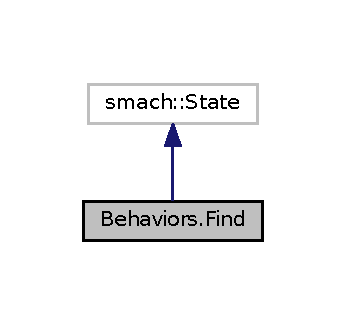
\includegraphics[width=166pt]{classBehaviors_1_1Find__inherit__graph}
\end{center}
\end{figure}


Collaboration diagram for Behaviors.\+Find\+:\nopagebreak
\begin{figure}[H]
\begin{center}
\leavevmode
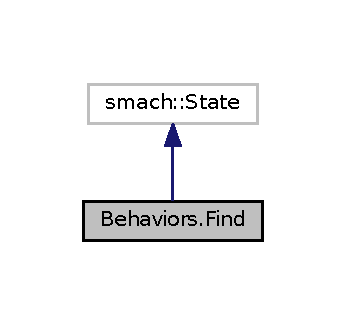
\includegraphics[width=166pt]{classBehaviors_1_1Find__coll__graph}
\end{center}
\end{figure}
\subsection*{Public Member Functions}
\begin{DoxyCompactItemize}
\item 
def {\bfseries \+\_\+\+\_\+init\+\_\+\+\_\+} (self)\hypertarget{classBehaviors_1_1Find_a50fe385da0196f85d03c9215531e8468}{}\label{classBehaviors_1_1Find_a50fe385da0196f85d03c9215531e8468}

\item 
def {\bfseries execute} (self, userdata)\hypertarget{classBehaviors_1_1Find_a4910773265944430bb02fc53318fb956}{}\label{classBehaviors_1_1Find_a4910773265944430bb02fc53318fb956}

\end{DoxyCompactItemize}


\subsection{Detailed Description}
\hyperlink{classBehaviors_1_1Find}{Find}\+: class that describes the \hyperlink{classBehaviors_1_1Find}{Find} state. 

The documentation for this class was generated from the following file\+:\begin{DoxyCompactItemize}
\item 
exp\+\_\+assignment3/scripts/Behaviors.\+py\end{DoxyCompactItemize}

\hypertarget{structfrontier__exploration_1_1Frontier}{}\section{frontier\+\_\+exploration\+:\+:Frontier Struct Reference}
\label{structfrontier__exploration_1_1Frontier}\index{frontier\+\_\+exploration\+::\+Frontier@{frontier\+\_\+exploration\+::\+Frontier}}


Represents a frontier.  




{\ttfamily \#include $<$frontier\+\_\+search.\+h$>$}

\subsection*{Public Attributes}
\begin{DoxyCompactItemize}
\item 
std\+::uint32\+\_\+t \hyperlink{structfrontier__exploration_1_1Frontier_ab850ad2ae90bf0308cba48ad9d8dec4c}{size}
\item 
double \hyperlink{structfrontier__exploration_1_1Frontier_a9d55b8e1c1276ad52d303e350eb01b36}{min\+\_\+distance}
\item 
double \hyperlink{structfrontier__exploration_1_1Frontier_a83107d241973d2a9ed3e182d590e7e56}{cost}
\item 
geometry\+\_\+msgs\+::\+Point \hyperlink{structfrontier__exploration_1_1Frontier_a21da5044337952793443ac74b2fdf1cb}{initial}
\item 
geometry\+\_\+msgs\+::\+Point \hyperlink{structfrontier__exploration_1_1Frontier_a45d35b7dc180ce9382630d9348f722db}{centroid}
\item 
geometry\+\_\+msgs\+::\+Point \hyperlink{structfrontier__exploration_1_1Frontier_a76f982fcee65872b354225b95f00ee5b}{middle}
\item 
std\+::vector$<$ geometry\+\_\+msgs\+::\+Point $>$ \hyperlink{structfrontier__exploration_1_1Frontier_ad124fa5a17e45fedd9e9b00d34182ea3}{points}
\end{DoxyCompactItemize}


\subsection{Detailed Description}
Represents a frontier. 

\subsection{Member Data Documentation}
\index{frontier\+\_\+exploration\+::\+Frontier@{frontier\+\_\+exploration\+::\+Frontier}!centroid@{centroid}}
\index{centroid@{centroid}!frontier\+\_\+exploration\+::\+Frontier@{frontier\+\_\+exploration\+::\+Frontier}}
\subsubsection[{\texorpdfstring{centroid}{centroid}}]{\setlength{\rightskip}{0pt plus 5cm}geometry\+\_\+msgs\+::\+Point frontier\+\_\+exploration\+::\+Frontier\+::centroid}\hypertarget{structfrontier__exploration_1_1Frontier_a45d35b7dc180ce9382630d9348f722db}{}\label{structfrontier__exploration_1_1Frontier_a45d35b7dc180ce9382630d9348f722db}
\index{frontier\+\_\+exploration\+::\+Frontier@{frontier\+\_\+exploration\+::\+Frontier}!cost@{cost}}
\index{cost@{cost}!frontier\+\_\+exploration\+::\+Frontier@{frontier\+\_\+exploration\+::\+Frontier}}
\subsubsection[{\texorpdfstring{cost}{cost}}]{\setlength{\rightskip}{0pt plus 5cm}double frontier\+\_\+exploration\+::\+Frontier\+::cost}\hypertarget{structfrontier__exploration_1_1Frontier_a83107d241973d2a9ed3e182d590e7e56}{}\label{structfrontier__exploration_1_1Frontier_a83107d241973d2a9ed3e182d590e7e56}
\index{frontier\+\_\+exploration\+::\+Frontier@{frontier\+\_\+exploration\+::\+Frontier}!initial@{initial}}
\index{initial@{initial}!frontier\+\_\+exploration\+::\+Frontier@{frontier\+\_\+exploration\+::\+Frontier}}
\subsubsection[{\texorpdfstring{initial}{initial}}]{\setlength{\rightskip}{0pt plus 5cm}geometry\+\_\+msgs\+::\+Point frontier\+\_\+exploration\+::\+Frontier\+::initial}\hypertarget{structfrontier__exploration_1_1Frontier_a21da5044337952793443ac74b2fdf1cb}{}\label{structfrontier__exploration_1_1Frontier_a21da5044337952793443ac74b2fdf1cb}
\index{frontier\+\_\+exploration\+::\+Frontier@{frontier\+\_\+exploration\+::\+Frontier}!middle@{middle}}
\index{middle@{middle}!frontier\+\_\+exploration\+::\+Frontier@{frontier\+\_\+exploration\+::\+Frontier}}
\subsubsection[{\texorpdfstring{middle}{middle}}]{\setlength{\rightskip}{0pt plus 5cm}geometry\+\_\+msgs\+::\+Point frontier\+\_\+exploration\+::\+Frontier\+::middle}\hypertarget{structfrontier__exploration_1_1Frontier_a76f982fcee65872b354225b95f00ee5b}{}\label{structfrontier__exploration_1_1Frontier_a76f982fcee65872b354225b95f00ee5b}
\index{frontier\+\_\+exploration\+::\+Frontier@{frontier\+\_\+exploration\+::\+Frontier}!min\+\_\+distance@{min\+\_\+distance}}
\index{min\+\_\+distance@{min\+\_\+distance}!frontier\+\_\+exploration\+::\+Frontier@{frontier\+\_\+exploration\+::\+Frontier}}
\subsubsection[{\texorpdfstring{min\+\_\+distance}{min_distance}}]{\setlength{\rightskip}{0pt plus 5cm}double frontier\+\_\+exploration\+::\+Frontier\+::min\+\_\+distance}\hypertarget{structfrontier__exploration_1_1Frontier_a9d55b8e1c1276ad52d303e350eb01b36}{}\label{structfrontier__exploration_1_1Frontier_a9d55b8e1c1276ad52d303e350eb01b36}
\index{frontier\+\_\+exploration\+::\+Frontier@{frontier\+\_\+exploration\+::\+Frontier}!points@{points}}
\index{points@{points}!frontier\+\_\+exploration\+::\+Frontier@{frontier\+\_\+exploration\+::\+Frontier}}
\subsubsection[{\texorpdfstring{points}{points}}]{\setlength{\rightskip}{0pt plus 5cm}std\+::vector$<$geometry\+\_\+msgs\+::\+Point$>$ frontier\+\_\+exploration\+::\+Frontier\+::points}\hypertarget{structfrontier__exploration_1_1Frontier_ad124fa5a17e45fedd9e9b00d34182ea3}{}\label{structfrontier__exploration_1_1Frontier_ad124fa5a17e45fedd9e9b00d34182ea3}
\index{frontier\+\_\+exploration\+::\+Frontier@{frontier\+\_\+exploration\+::\+Frontier}!size@{size}}
\index{size@{size}!frontier\+\_\+exploration\+::\+Frontier@{frontier\+\_\+exploration\+::\+Frontier}}
\subsubsection[{\texorpdfstring{size}{size}}]{\setlength{\rightskip}{0pt plus 5cm}std\+::uint32\+\_\+t frontier\+\_\+exploration\+::\+Frontier\+::size}\hypertarget{structfrontier__exploration_1_1Frontier_ab850ad2ae90bf0308cba48ad9d8dec4c}{}\label{structfrontier__exploration_1_1Frontier_ab850ad2ae90bf0308cba48ad9d8dec4c}


The documentation for this struct was generated from the following file\+:\begin{DoxyCompactItemize}
\item 
m-\/explore/explore/include/explore/\hyperlink{frontier__search_8h}{frontier\+\_\+search.\+h}\end{DoxyCompactItemize}

\hypertarget{classfrontier__exploration_1_1FrontierSearch}{}\section{frontier\+\_\+exploration\+:\+:Frontier\+Search Class Reference}
\label{classfrontier__exploration_1_1FrontierSearch}\index{frontier\+\_\+exploration\+::\+Frontier\+Search@{frontier\+\_\+exploration\+::\+Frontier\+Search}}


Thread-\/safe implementation of a frontier-\/search task for an input costmap.  




{\ttfamily \#include $<$frontier\+\_\+search.\+h$>$}

\subsection*{Public Member Functions}
\begin{DoxyCompactItemize}
\item 
\hyperlink{classfrontier__exploration_1_1FrontierSearch_a3396c0bfc5f1c545ae4be16068eeb620}{Frontier\+Search} ()
\item 
\hyperlink{classfrontier__exploration_1_1FrontierSearch_a0d07b12823e27600de8405d652e9a69a}{Frontier\+Search} (costmap\+\_\+2d\+::\+Costmap2D $\ast$costmap, double potential\+\_\+scale, double gain\+\_\+scale, double min\+\_\+frontier\+\_\+size)
\begin{DoxyCompactList}\small\item\em Constructor for search task. \end{DoxyCompactList}\item 
std\+::vector$<$ \hyperlink{structfrontier__exploration_1_1Frontier}{Frontier} $>$ \hyperlink{classfrontier__exploration_1_1FrontierSearch_ac28ed3ce13ab687ed002f74338189f48}{search\+From} (geometry\+\_\+msgs\+::\+Point position)
\begin{DoxyCompactList}\small\item\em Runs search implementation, outward from the start position. \end{DoxyCompactList}\end{DoxyCompactItemize}
\subsection*{Protected Member Functions}
\begin{DoxyCompactItemize}
\item 
\hyperlink{structfrontier__exploration_1_1Frontier}{Frontier} \hyperlink{classfrontier__exploration_1_1FrontierSearch_a03ab2174fbd43e117cd816aade7d3b38}{build\+New\+Frontier} (unsigned int initial\+\_\+cell, unsigned int reference, std\+::vector$<$ bool $>$ \&frontier\+\_\+flag)
\begin{DoxyCompactList}\small\item\em Starting from an initial cell, build a frontier from valid adjacent cells. \end{DoxyCompactList}\item 
bool \hyperlink{classfrontier__exploration_1_1FrontierSearch_a4fc0a3e7d14dd1bcab5aa67bae684350}{is\+New\+Frontier\+Cell} (unsigned int idx, const std\+::vector$<$ bool $>$ \&frontier\+\_\+flag)
\begin{DoxyCompactList}\small\item\em is\+New\+Frontier\+Cell Evaluate if candidate cell is a valid candidate for a new frontier. \end{DoxyCompactList}\item 
double \hyperlink{classfrontier__exploration_1_1FrontierSearch_a46cf94258988537430a3425140803e59}{frontier\+Cost} (const \hyperlink{structfrontier__exploration_1_1Frontier}{Frontier} \&frontier)
\begin{DoxyCompactList}\small\item\em computes frontier cost \end{DoxyCompactList}\end{DoxyCompactItemize}


\subsection{Detailed Description}
Thread-\/safe implementation of a frontier-\/search task for an input costmap. 

\subsection{Constructor \& Destructor Documentation}
\index{frontier\+\_\+exploration\+::\+Frontier\+Search@{frontier\+\_\+exploration\+::\+Frontier\+Search}!Frontier\+Search@{Frontier\+Search}}
\index{Frontier\+Search@{Frontier\+Search}!frontier\+\_\+exploration\+::\+Frontier\+Search@{frontier\+\_\+exploration\+::\+Frontier\+Search}}
\subsubsection[{\texorpdfstring{Frontier\+Search()}{FrontierSearch()}}]{\setlength{\rightskip}{0pt plus 5cm}frontier\+\_\+exploration\+::\+Frontier\+Search\+::\+Frontier\+Search (
\begin{DoxyParamCaption}
{}
\end{DoxyParamCaption}
)\hspace{0.3cm}{\ttfamily [inline]}}\hypertarget{classfrontier__exploration_1_1FrontierSearch_a3396c0bfc5f1c545ae4be16068eeb620}{}\label{classfrontier__exploration_1_1FrontierSearch_a3396c0bfc5f1c545ae4be16068eeb620}
\index{frontier\+\_\+exploration\+::\+Frontier\+Search@{frontier\+\_\+exploration\+::\+Frontier\+Search}!Frontier\+Search@{Frontier\+Search}}
\index{Frontier\+Search@{Frontier\+Search}!frontier\+\_\+exploration\+::\+Frontier\+Search@{frontier\+\_\+exploration\+::\+Frontier\+Search}}
\subsubsection[{\texorpdfstring{Frontier\+Search(costmap\+\_\+2d\+::\+Costmap2\+D $\ast$costmap, double potential\+\_\+scale, double gain\+\_\+scale, double min\+\_\+frontier\+\_\+size)}{FrontierSearch(costmap_2d::Costmap2D *costmap, double potential_scale, double gain_scale, double min_frontier_size)}}]{\setlength{\rightskip}{0pt plus 5cm}frontier\+\_\+exploration\+::\+Frontier\+Search\+::\+Frontier\+Search (
\begin{DoxyParamCaption}
\item[{costmap\+\_\+2d\+::\+Costmap2D $\ast$}]{costmap, }
\item[{double}]{potential\+\_\+scale, }
\item[{double}]{gain\+\_\+scale, }
\item[{double}]{min\+\_\+frontier\+\_\+size}
\end{DoxyParamCaption}
)}\hypertarget{classfrontier__exploration_1_1FrontierSearch_a0d07b12823e27600de8405d652e9a69a}{}\label{classfrontier__exploration_1_1FrontierSearch_a0d07b12823e27600de8405d652e9a69a}


Constructor for search task. 


\begin{DoxyParams}{Parameters}
{\em costmap} & Reference to costmap data to search. \\
\hline
\end{DoxyParams}


\subsection{Member Function Documentation}
\index{frontier\+\_\+exploration\+::\+Frontier\+Search@{frontier\+\_\+exploration\+::\+Frontier\+Search}!build\+New\+Frontier@{build\+New\+Frontier}}
\index{build\+New\+Frontier@{build\+New\+Frontier}!frontier\+\_\+exploration\+::\+Frontier\+Search@{frontier\+\_\+exploration\+::\+Frontier\+Search}}
\subsubsection[{\texorpdfstring{build\+New\+Frontier(unsigned int initial\+\_\+cell, unsigned int reference, std\+::vector$<$ bool $>$ \&frontier\+\_\+flag)}{buildNewFrontier(unsigned int initial_cell, unsigned int reference, std::vector< bool > &frontier_flag)}}]{\setlength{\rightskip}{0pt plus 5cm}{\bf Frontier} frontier\+\_\+exploration\+::\+Frontier\+Search\+::build\+New\+Frontier (
\begin{DoxyParamCaption}
\item[{unsigned int}]{initial\+\_\+cell, }
\item[{unsigned int}]{reference, }
\item[{std\+::vector$<$ bool $>$ \&}]{frontier\+\_\+flag}
\end{DoxyParamCaption}
)\hspace{0.3cm}{\ttfamily [protected]}}\hypertarget{classfrontier__exploration_1_1FrontierSearch_a03ab2174fbd43e117cd816aade7d3b38}{}\label{classfrontier__exploration_1_1FrontierSearch_a03ab2174fbd43e117cd816aade7d3b38}


Starting from an initial cell, build a frontier from valid adjacent cells. 


\begin{DoxyParams}{Parameters}
{\em initial\+\_\+cell} & Index of cell to start frontier building \\
\hline
{\em reference} & Reference index to calculate position from \\
\hline
{\em frontier\+\_\+flag} & Flag vector indicating which cells are already marked as frontiers \\
\hline
\end{DoxyParams}
\begin{DoxyReturn}{Returns}
new frontier 
\end{DoxyReturn}
\index{frontier\+\_\+exploration\+::\+Frontier\+Search@{frontier\+\_\+exploration\+::\+Frontier\+Search}!frontier\+Cost@{frontier\+Cost}}
\index{frontier\+Cost@{frontier\+Cost}!frontier\+\_\+exploration\+::\+Frontier\+Search@{frontier\+\_\+exploration\+::\+Frontier\+Search}}
\subsubsection[{\texorpdfstring{frontier\+Cost(const Frontier \&frontier)}{frontierCost(const Frontier &frontier)}}]{\setlength{\rightskip}{0pt plus 5cm}double frontier\+\_\+exploration\+::\+Frontier\+Search\+::frontier\+Cost (
\begin{DoxyParamCaption}
\item[{const {\bf Frontier} \&}]{frontier}
\end{DoxyParamCaption}
)\hspace{0.3cm}{\ttfamily [protected]}}\hypertarget{classfrontier__exploration_1_1FrontierSearch_a46cf94258988537430a3425140803e59}{}\label{classfrontier__exploration_1_1FrontierSearch_a46cf94258988537430a3425140803e59}


computes frontier cost 

cost function is defined by potential\+\_\+scale and gain\+\_\+scale


\begin{DoxyParams}{Parameters}
{\em frontier} & frontier for which compute the cost \\
\hline
\end{DoxyParams}
\begin{DoxyReturn}{Returns}
cost of the frontier 
\end{DoxyReturn}
\index{frontier\+\_\+exploration\+::\+Frontier\+Search@{frontier\+\_\+exploration\+::\+Frontier\+Search}!is\+New\+Frontier\+Cell@{is\+New\+Frontier\+Cell}}
\index{is\+New\+Frontier\+Cell@{is\+New\+Frontier\+Cell}!frontier\+\_\+exploration\+::\+Frontier\+Search@{frontier\+\_\+exploration\+::\+Frontier\+Search}}
\subsubsection[{\texorpdfstring{is\+New\+Frontier\+Cell(unsigned int idx, const std\+::vector$<$ bool $>$ \&frontier\+\_\+flag)}{isNewFrontierCell(unsigned int idx, const std::vector< bool > &frontier_flag)}}]{\setlength{\rightskip}{0pt plus 5cm}bool frontier\+\_\+exploration\+::\+Frontier\+Search\+::is\+New\+Frontier\+Cell (
\begin{DoxyParamCaption}
\item[{unsigned int}]{idx, }
\item[{const std\+::vector$<$ bool $>$ \&}]{frontier\+\_\+flag}
\end{DoxyParamCaption}
)\hspace{0.3cm}{\ttfamily [protected]}}\hypertarget{classfrontier__exploration_1_1FrontierSearch_a4fc0a3e7d14dd1bcab5aa67bae684350}{}\label{classfrontier__exploration_1_1FrontierSearch_a4fc0a3e7d14dd1bcab5aa67bae684350}


is\+New\+Frontier\+Cell Evaluate if candidate cell is a valid candidate for a new frontier. 


\begin{DoxyParams}{Parameters}
{\em idx} & Index of candidate cell \\
\hline
{\em frontier\+\_\+flag} & Flag vector indicating which cells are already marked as frontiers \\
\hline
\end{DoxyParams}
\begin{DoxyReturn}{Returns}
true if the cell is frontier cell 
\end{DoxyReturn}
\index{frontier\+\_\+exploration\+::\+Frontier\+Search@{frontier\+\_\+exploration\+::\+Frontier\+Search}!search\+From@{search\+From}}
\index{search\+From@{search\+From}!frontier\+\_\+exploration\+::\+Frontier\+Search@{frontier\+\_\+exploration\+::\+Frontier\+Search}}
\subsubsection[{\texorpdfstring{search\+From(geometry\+\_\+msgs\+::\+Point position)}{searchFrom(geometry_msgs::Point position)}}]{\setlength{\rightskip}{0pt plus 5cm}std\+::vector$<$ {\bf Frontier} $>$ frontier\+\_\+exploration\+::\+Frontier\+Search\+::search\+From (
\begin{DoxyParamCaption}
\item[{geometry\+\_\+msgs\+::\+Point}]{position}
\end{DoxyParamCaption}
)}\hypertarget{classfrontier__exploration_1_1FrontierSearch_ac28ed3ce13ab687ed002f74338189f48}{}\label{classfrontier__exploration_1_1FrontierSearch_ac28ed3ce13ab687ed002f74338189f48}


Runs search implementation, outward from the start position. 


\begin{DoxyParams}{Parameters}
{\em position} & Initial position to search from \\
\hline
\end{DoxyParams}
\begin{DoxyReturn}{Returns}
List of frontiers, if any 
\end{DoxyReturn}


The documentation for this class was generated from the following files\+:\begin{DoxyCompactItemize}
\item 
m-\/explore/explore/include/explore/\hyperlink{frontier__search_8h}{frontier\+\_\+search.\+h}\item 
m-\/explore/explore/src/\hyperlink{frontier__search_8cpp}{frontier\+\_\+search.\+cpp}\end{DoxyCompactItemize}

\hypertarget{classPerception_1_1image__feature}{}\section{Perception.\+image\+\_\+feature Class Reference}
\label{classPerception_1_1image__feature}\index{Perception.\+image\+\_\+feature@{Perception.\+image\+\_\+feature}}


C\+L\+A\+SS.  


\subsection*{Public Member Functions}
\begin{DoxyCompactItemize}
\item 
def \hyperlink{classPerception_1_1image__feature_a748b3574bea982b0e5b29a86dfca644e}{\+\_\+\+\_\+init\+\_\+\+\_\+} (self)
\item 
def {\bfseries callback} (self, ros\+\_\+data)\hypertarget{classPerception_1_1image__feature_aa4163f3a9600d001cfd6ac90ba460df9}{}\label{classPerception_1_1image__feature_aa4163f3a9600d001cfd6ac90ba460df9}

\end{DoxyCompactItemize}
\subsection*{Public Attributes}
\begin{DoxyCompactItemize}
\item 
{\bfseries image\+\_\+pub}\hypertarget{classPerception_1_1image__feature_acfc602315032d7e877533594d93ed051}{}\label{classPerception_1_1image__feature_acfc602315032d7e877533594d93ed051}

\item 
{\bfseries vel\+\_\+pub}\hypertarget{classPerception_1_1image__feature_a2582bcb9aca24ef19e5a249684048c84}{}\label{classPerception_1_1image__feature_a2582bcb9aca24ef19e5a249684048c84}

\item 
{\bfseries subscriber}\hypertarget{classPerception_1_1image__feature_a73606194793aca7799100ae95535b072}{}\label{classPerception_1_1image__feature_a73606194793aca7799100ae95535b072}

\end{DoxyCompactItemize}


\subsection{Detailed Description}
C\+L\+A\+SS. 

Image feature class to handle feature identification inside the image sent by the camera 

\subsection{Constructor \& Destructor Documentation}
\index{Perception\+::image\+\_\+feature@{Perception\+::image\+\_\+feature}!\+\_\+\+\_\+init\+\_\+\+\_\+@{\+\_\+\+\_\+init\+\_\+\+\_\+}}
\index{\+\_\+\+\_\+init\+\_\+\+\_\+@{\+\_\+\+\_\+init\+\_\+\+\_\+}!Perception\+::image\+\_\+feature@{Perception\+::image\+\_\+feature}}
\subsubsection[{\texorpdfstring{\+\_\+\+\_\+init\+\_\+\+\_\+(self)}{__init__(self)}}]{\setlength{\rightskip}{0pt plus 5cm}def Perception.\+image\+\_\+feature.\+\_\+\+\_\+init\+\_\+\+\_\+ (
\begin{DoxyParamCaption}
\item[{}]{self}
\end{DoxyParamCaption}
)}\hypertarget{classPerception_1_1image__feature_a748b3574bea982b0e5b29a86dfca644e}{}\label{classPerception_1_1image__feature_a748b3574bea982b0e5b29a86dfca644e}
\begin{DoxyVerb}Initialize ros publisher, ros subscriber\end{DoxyVerb}
 

The documentation for this class was generated from the following file\+:\begin{DoxyCompactItemize}
\item 
exp\+\_\+assignment3/scripts/Perception.\+py\end{DoxyCompactItemize}

\hypertarget{classBehaviors_1_1Normal}{}\section{Behaviors.\+Normal Class Reference}
\label{classBehaviors_1_1Normal}\index{Behaviors.\+Normal@{Behaviors.\+Normal}}


\hyperlink{classBehaviors_1_1Normal}{Normal}\+: class that describes the \hyperlink{classBehaviors_1_1Normal}{Normal} state.  




Inheritance diagram for Behaviors.\+Normal\+:\nopagebreak
\begin{figure}[H]
\begin{center}
\leavevmode
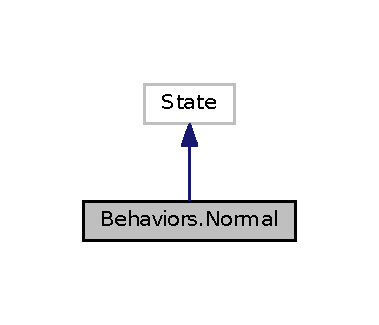
\includegraphics[width=182pt]{classBehaviors_1_1Normal__inherit__graph}
\end{center}
\end{figure}


Collaboration diagram for Behaviors.\+Normal\+:\nopagebreak
\begin{figure}[H]
\begin{center}
\leavevmode
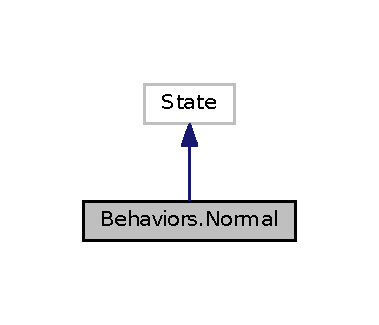
\includegraphics[width=182pt]{classBehaviors_1_1Normal__coll__graph}
\end{center}
\end{figure}
\subsection*{Public Member Functions}
\begin{DoxyCompactItemize}
\item 
def \hyperlink{classBehaviors_1_1Normal_a0d48c743470e9356c7eec875add25d1d}{\+\_\+\+\_\+init\+\_\+\+\_\+} (self)
\item 
def \hyperlink{classBehaviors_1_1Normal_ad85b58cb3f66b79ca64036abf251d191}{execute} (self, userdata)
\end{DoxyCompactItemize}


\subsection{Detailed Description}
\hyperlink{classBehaviors_1_1Normal}{Normal}\+: class that describes the \hyperlink{classBehaviors_1_1Normal}{Normal} state. 

\subsection{Constructor \& Destructor Documentation}
\index{Behaviors\+::\+Normal@{Behaviors\+::\+Normal}!\+\_\+\+\_\+init\+\_\+\+\_\+@{\+\_\+\+\_\+init\+\_\+\+\_\+}}
\index{\+\_\+\+\_\+init\+\_\+\+\_\+@{\+\_\+\+\_\+init\+\_\+\+\_\+}!Behaviors\+::\+Normal@{Behaviors\+::\+Normal}}
\subsubsection[{\texorpdfstring{\+\_\+\+\_\+init\+\_\+\+\_\+(self)}{__init__(self)}}]{\setlength{\rightskip}{0pt plus 5cm}def Behaviors.\+Normal.\+\_\+\+\_\+init\+\_\+\+\_\+ (
\begin{DoxyParamCaption}
\item[{}]{self}
\end{DoxyParamCaption}
)}\hypertarget{classBehaviors_1_1Normal_a0d48c743470e9356c7eec875add25d1d}{}\label{classBehaviors_1_1Normal_a0d48c743470e9356c7eec875add25d1d}


\subsection{Member Function Documentation}
\index{Behaviors\+::\+Normal@{Behaviors\+::\+Normal}!execute@{execute}}
\index{execute@{execute}!Behaviors\+::\+Normal@{Behaviors\+::\+Normal}}
\subsubsection[{\texorpdfstring{execute(self, userdata)}{execute(self, userdata)}}]{\setlength{\rightskip}{0pt plus 5cm}def Behaviors.\+Normal.\+execute (
\begin{DoxyParamCaption}
\item[{}]{self, }
\item[{}]{userdata}
\end{DoxyParamCaption}
)}\hypertarget{classBehaviors_1_1Normal_ad85b58cb3f66b79ca64036abf251d191}{}\label{classBehaviors_1_1Normal_ad85b58cb3f66b79ca64036abf251d191}


The documentation for this class was generated from the following file\+:\begin{DoxyCompactItemize}
\item 
exp\+\_\+assignment3/scripts/\hyperlink{Behaviors_8py}{Behaviors.\+py}\end{DoxyCompactItemize}

\hypertarget{classBehaviors_1_1Play}{}\section{Behaviors.\+Play Class Reference}
\label{classBehaviors_1_1Play}\index{Behaviors.\+Play@{Behaviors.\+Play}}


\hyperlink{classBehaviors_1_1Play}{Play}\+: class that describes the \hyperlink{classBehaviors_1_1Play}{Play} state.  




Inheritance diagram for Behaviors.\+Play\+:\nopagebreak
\begin{figure}[H]
\begin{center}
\leavevmode
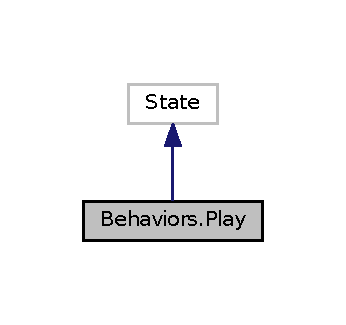
\includegraphics[width=166pt]{classBehaviors_1_1Play__inherit__graph}
\end{center}
\end{figure}


Collaboration diagram for Behaviors.\+Play\+:\nopagebreak
\begin{figure}[H]
\begin{center}
\leavevmode
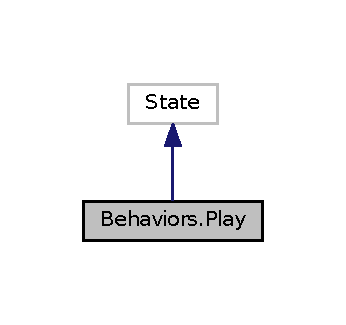
\includegraphics[width=166pt]{classBehaviors_1_1Play__coll__graph}
\end{center}
\end{figure}
\subsection*{Public Member Functions}
\begin{DoxyCompactItemize}
\item 
def {\bfseries \+\_\+\+\_\+init\+\_\+\+\_\+} (self)\hypertarget{classBehaviors_1_1Play_a5a5684ee3c87670a8eeeadb57ecba0d3}{}\label{classBehaviors_1_1Play_a5a5684ee3c87670a8eeeadb57ecba0d3}

\item 
def {\bfseries execute} (self, userdata)\hypertarget{classBehaviors_1_1Play_a2c8c1be112cceeb3b11c2450755306fe}{}\label{classBehaviors_1_1Play_a2c8c1be112cceeb3b11c2450755306fe}

\end{DoxyCompactItemize}


\subsection{Detailed Description}
\hyperlink{classBehaviors_1_1Play}{Play}\+: class that describes the \hyperlink{classBehaviors_1_1Play}{Play} state. 

The documentation for this class was generated from the following file\+:\begin{DoxyCompactItemize}
\item 
exp\+\_\+assignment3/scripts/Behaviors.\+py\end{DoxyCompactItemize}

\hypertarget{classBehaviors_1_1Recovery}{}\section{Behaviors.\+Recovery Class Reference}
\label{classBehaviors_1_1Recovery}\index{Behaviors.\+Recovery@{Behaviors.\+Recovery}}


\hyperlink{classBehaviors_1_1Recovery}{Recovery}\+: class that describes the \hyperlink{classBehaviors_1_1Recovery}{Recovery} state.  




Inheritance diagram for Behaviors.\+Recovery\+:\nopagebreak
\begin{figure}[H]
\begin{center}
\leavevmode
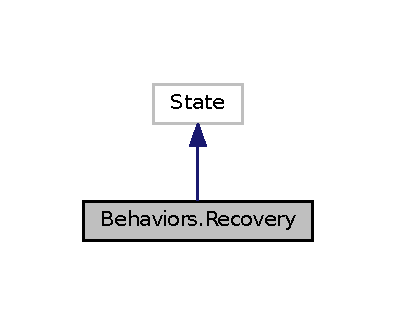
\includegraphics[width=190pt]{classBehaviors_1_1Recovery__inherit__graph}
\end{center}
\end{figure}


Collaboration diagram for Behaviors.\+Recovery\+:\nopagebreak
\begin{figure}[H]
\begin{center}
\leavevmode
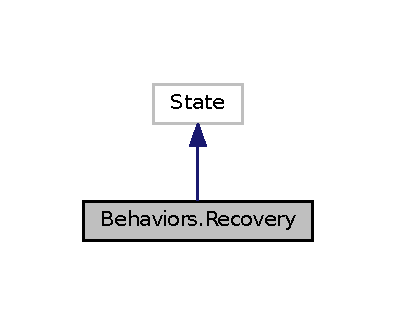
\includegraphics[width=190pt]{classBehaviors_1_1Recovery__coll__graph}
\end{center}
\end{figure}
\subsection*{Public Member Functions}
\begin{DoxyCompactItemize}
\item 
def \hyperlink{classBehaviors_1_1Recovery_a9952b507236ae466b701935a6e2482d6}{\+\_\+\+\_\+init\+\_\+\+\_\+} (self)
\item 
def \hyperlink{classBehaviors_1_1Recovery_a83ad65d2d9ca8efabb0c9977c8b8449a}{execute} (self, userdata)
\end{DoxyCompactItemize}


\subsection{Detailed Description}
\hyperlink{classBehaviors_1_1Recovery}{Recovery}\+: class that describes the \hyperlink{classBehaviors_1_1Recovery}{Recovery} state. 

\subsection{Constructor \& Destructor Documentation}
\index{Behaviors\+::\+Recovery@{Behaviors\+::\+Recovery}!\+\_\+\+\_\+init\+\_\+\+\_\+@{\+\_\+\+\_\+init\+\_\+\+\_\+}}
\index{\+\_\+\+\_\+init\+\_\+\+\_\+@{\+\_\+\+\_\+init\+\_\+\+\_\+}!Behaviors\+::\+Recovery@{Behaviors\+::\+Recovery}}
\subsubsection[{\texorpdfstring{\+\_\+\+\_\+init\+\_\+\+\_\+(self)}{__init__(self)}}]{\setlength{\rightskip}{0pt plus 5cm}def Behaviors.\+Recovery.\+\_\+\+\_\+init\+\_\+\+\_\+ (
\begin{DoxyParamCaption}
\item[{}]{self}
\end{DoxyParamCaption}
)}\hypertarget{classBehaviors_1_1Recovery_a9952b507236ae466b701935a6e2482d6}{}\label{classBehaviors_1_1Recovery_a9952b507236ae466b701935a6e2482d6}


\subsection{Member Function Documentation}
\index{Behaviors\+::\+Recovery@{Behaviors\+::\+Recovery}!execute@{execute}}
\index{execute@{execute}!Behaviors\+::\+Recovery@{Behaviors\+::\+Recovery}}
\subsubsection[{\texorpdfstring{execute(self, userdata)}{execute(self, userdata)}}]{\setlength{\rightskip}{0pt plus 5cm}def Behaviors.\+Recovery.\+execute (
\begin{DoxyParamCaption}
\item[{}]{self, }
\item[{}]{userdata}
\end{DoxyParamCaption}
)}\hypertarget{classBehaviors_1_1Recovery_a83ad65d2d9ca8efabb0c9977c8b8449a}{}\label{classBehaviors_1_1Recovery_a83ad65d2d9ca8efabb0c9977c8b8449a}


The documentation for this class was generated from the following file\+:\begin{DoxyCompactItemize}
\item 
exp\+\_\+assignment3/scripts/\hyperlink{Behaviors_8py}{Behaviors.\+py}\end{DoxyCompactItemize}

\hypertarget{classSlamGMapping}{}\section{Slam\+G\+Mapping Class Reference}
\label{classSlamGMapping}\index{Slam\+G\+Mapping@{Slam\+G\+Mapping}}


{\ttfamily \#include $<$slam\+\_\+gmapping.\+h$>$}

\subsection*{Public Member Functions}
\begin{DoxyCompactItemize}
\item 
\hyperlink{classSlamGMapping_aa40ca229b3db4d0cf5bf7448c475a4c3}{Slam\+G\+Mapping} ()
\item 
\hyperlink{classSlamGMapping_a3f9432f78c6eff17041a4b0b0f87a1ad}{Slam\+G\+Mapping} (ros\+::\+Node\+Handle \&nh, ros\+::\+Node\+Handle \&pnh)
\item 
\hyperlink{classSlamGMapping_a6a4853715facc1ee2591955180e830a2}{Slam\+G\+Mapping} (unsigned long int seed, unsigned long int max\+\_\+duration\+\_\+buffer)
\item 
\hyperlink{classSlamGMapping_ae4a539b79ee1f11b7430f313ad445667}{$\sim$\+Slam\+G\+Mapping} ()
\item 
void \hyperlink{classSlamGMapping_aca7f6aaa57c8ac675068701adda348ea}{init} ()
\item 
void \hyperlink{classSlamGMapping_ab0d5567e7a8e010ff11068fcce0d9c04}{start\+Live\+Slam} ()
\item 
void \hyperlink{classSlamGMapping_a90bee18e7c96af13916caae4a4bfd618}{start\+Replay} (const std\+::string \&bag\+\_\+fname, std\+::string scan\+\_\+topic)
\item 
void \hyperlink{classSlamGMapping_a2447af8faad253af05c7dc9f492b8489}{publish\+Transform} ()
\item 
void \hyperlink{classSlamGMapping_a49172a6ae33df4daf397959789dc1c34}{laser\+Callback} (const sensor\+\_\+msgs\+::\+Laser\+Scan\+::\+Const\+Ptr \&scan)
\item 
bool \hyperlink{classSlamGMapping_a780899c48f753bf4768580fb46580d83}{map\+Callback} (nav\+\_\+msgs\+::\+Get\+Map\+::\+Request \&req, nav\+\_\+msgs\+::\+Get\+Map\+::\+Response \&res)
\item 
void \hyperlink{classSlamGMapping_a00a01ecfacccbfcfccc3e138de6bd00f}{publish\+Loop} (double transform\+\_\+publish\+\_\+period)
\end{DoxyCompactItemize}


\subsection{Constructor \& Destructor Documentation}
\index{Slam\+G\+Mapping@{Slam\+G\+Mapping}!Slam\+G\+Mapping@{Slam\+G\+Mapping}}
\index{Slam\+G\+Mapping@{Slam\+G\+Mapping}!Slam\+G\+Mapping@{Slam\+G\+Mapping}}
\subsubsection[{\texorpdfstring{Slam\+G\+Mapping()}{SlamGMapping()}}]{\setlength{\rightskip}{0pt plus 5cm}Slam\+G\+Mapping\+::\+Slam\+G\+Mapping (
\begin{DoxyParamCaption}
{}
\end{DoxyParamCaption}
)}\hypertarget{classSlamGMapping_aa40ca229b3db4d0cf5bf7448c475a4c3}{}\label{classSlamGMapping_aa40ca229b3db4d0cf5bf7448c475a4c3}
\index{Slam\+G\+Mapping@{Slam\+G\+Mapping}!Slam\+G\+Mapping@{Slam\+G\+Mapping}}
\index{Slam\+G\+Mapping@{Slam\+G\+Mapping}!Slam\+G\+Mapping@{Slam\+G\+Mapping}}
\subsubsection[{\texorpdfstring{Slam\+G\+Mapping(ros\+::\+Node\+Handle \&nh, ros\+::\+Node\+Handle \&pnh)}{SlamGMapping(ros::NodeHandle &nh, ros::NodeHandle &pnh)}}]{\setlength{\rightskip}{0pt plus 5cm}Slam\+G\+Mapping\+::\+Slam\+G\+Mapping (
\begin{DoxyParamCaption}
\item[{ros\+::\+Node\+Handle \&}]{nh, }
\item[{ros\+::\+Node\+Handle \&}]{pnh}
\end{DoxyParamCaption}
)}\hypertarget{classSlamGMapping_a3f9432f78c6eff17041a4b0b0f87a1ad}{}\label{classSlamGMapping_a3f9432f78c6eff17041a4b0b0f87a1ad}
\index{Slam\+G\+Mapping@{Slam\+G\+Mapping}!Slam\+G\+Mapping@{Slam\+G\+Mapping}}
\index{Slam\+G\+Mapping@{Slam\+G\+Mapping}!Slam\+G\+Mapping@{Slam\+G\+Mapping}}
\subsubsection[{\texorpdfstring{Slam\+G\+Mapping(unsigned long int seed, unsigned long int max\+\_\+duration\+\_\+buffer)}{SlamGMapping(unsigned long int seed, unsigned long int max_duration_buffer)}}]{\setlength{\rightskip}{0pt plus 5cm}Slam\+G\+Mapping\+::\+Slam\+G\+Mapping (
\begin{DoxyParamCaption}
\item[{unsigned long int}]{seed, }
\item[{unsigned long int}]{max\+\_\+duration\+\_\+buffer}
\end{DoxyParamCaption}
)}\hypertarget{classSlamGMapping_a6a4853715facc1ee2591955180e830a2}{}\label{classSlamGMapping_a6a4853715facc1ee2591955180e830a2}
\index{Slam\+G\+Mapping@{Slam\+G\+Mapping}!````~Slam\+G\+Mapping@{$\sim$\+Slam\+G\+Mapping}}
\index{````~Slam\+G\+Mapping@{$\sim$\+Slam\+G\+Mapping}!Slam\+G\+Mapping@{Slam\+G\+Mapping}}
\subsubsection[{\texorpdfstring{$\sim$\+Slam\+G\+Mapping()}{~SlamGMapping()}}]{\setlength{\rightskip}{0pt plus 5cm}Slam\+G\+Mapping\+::$\sim$\+Slam\+G\+Mapping (
\begin{DoxyParamCaption}
{}
\end{DoxyParamCaption}
)}\hypertarget{classSlamGMapping_ae4a539b79ee1f11b7430f313ad445667}{}\label{classSlamGMapping_ae4a539b79ee1f11b7430f313ad445667}


\subsection{Member Function Documentation}
\index{Slam\+G\+Mapping@{Slam\+G\+Mapping}!init@{init}}
\index{init@{init}!Slam\+G\+Mapping@{Slam\+G\+Mapping}}
\subsubsection[{\texorpdfstring{init()}{init()}}]{\setlength{\rightskip}{0pt plus 5cm}void Slam\+G\+Mapping\+::init (
\begin{DoxyParamCaption}
{}
\end{DoxyParamCaption}
)}\hypertarget{classSlamGMapping_aca7f6aaa57c8ac675068701adda348ea}{}\label{classSlamGMapping_aca7f6aaa57c8ac675068701adda348ea}
\index{Slam\+G\+Mapping@{Slam\+G\+Mapping}!laser\+Callback@{laser\+Callback}}
\index{laser\+Callback@{laser\+Callback}!Slam\+G\+Mapping@{Slam\+G\+Mapping}}
\subsubsection[{\texorpdfstring{laser\+Callback(const sensor\+\_\+msgs\+::\+Laser\+Scan\+::\+Const\+Ptr \&scan)}{laserCallback(const sensor_msgs::LaserScan::ConstPtr &scan)}}]{\setlength{\rightskip}{0pt plus 5cm}void Slam\+G\+Mapping\+::laser\+Callback (
\begin{DoxyParamCaption}
\item[{const sensor\+\_\+msgs\+::\+Laser\+Scan\+::\+Const\+Ptr \&}]{scan}
\end{DoxyParamCaption}
)}\hypertarget{classSlamGMapping_a49172a6ae33df4daf397959789dc1c34}{}\label{classSlamGMapping_a49172a6ae33df4daf397959789dc1c34}
\index{Slam\+G\+Mapping@{Slam\+G\+Mapping}!map\+Callback@{map\+Callback}}
\index{map\+Callback@{map\+Callback}!Slam\+G\+Mapping@{Slam\+G\+Mapping}}
\subsubsection[{\texorpdfstring{map\+Callback(nav\+\_\+msgs\+::\+Get\+Map\+::\+Request \&req, nav\+\_\+msgs\+::\+Get\+Map\+::\+Response \&res)}{mapCallback(nav_msgs::GetMap::Request &req, nav_msgs::GetMap::Response &res)}}]{\setlength{\rightskip}{0pt plus 5cm}bool Slam\+G\+Mapping\+::map\+Callback (
\begin{DoxyParamCaption}
\item[{nav\+\_\+msgs\+::\+Get\+Map\+::\+Request \&}]{req, }
\item[{nav\+\_\+msgs\+::\+Get\+Map\+::\+Response \&}]{res}
\end{DoxyParamCaption}
)}\hypertarget{classSlamGMapping_a780899c48f753bf4768580fb46580d83}{}\label{classSlamGMapping_a780899c48f753bf4768580fb46580d83}
\index{Slam\+G\+Mapping@{Slam\+G\+Mapping}!publish\+Loop@{publish\+Loop}}
\index{publish\+Loop@{publish\+Loop}!Slam\+G\+Mapping@{Slam\+G\+Mapping}}
\subsubsection[{\texorpdfstring{publish\+Loop(double transform\+\_\+publish\+\_\+period)}{publishLoop(double transform_publish_period)}}]{\setlength{\rightskip}{0pt plus 5cm}void Slam\+G\+Mapping\+::publish\+Loop (
\begin{DoxyParamCaption}
\item[{double}]{transform\+\_\+publish\+\_\+period}
\end{DoxyParamCaption}
)}\hypertarget{classSlamGMapping_a00a01ecfacccbfcfccc3e138de6bd00f}{}\label{classSlamGMapping_a00a01ecfacccbfcfccc3e138de6bd00f}
\index{Slam\+G\+Mapping@{Slam\+G\+Mapping}!publish\+Transform@{publish\+Transform}}
\index{publish\+Transform@{publish\+Transform}!Slam\+G\+Mapping@{Slam\+G\+Mapping}}
\subsubsection[{\texorpdfstring{publish\+Transform()}{publishTransform()}}]{\setlength{\rightskip}{0pt plus 5cm}void Slam\+G\+Mapping\+::publish\+Transform (
\begin{DoxyParamCaption}
{}
\end{DoxyParamCaption}
)}\hypertarget{classSlamGMapping_a2447af8faad253af05c7dc9f492b8489}{}\label{classSlamGMapping_a2447af8faad253af05c7dc9f492b8489}
\index{Slam\+G\+Mapping@{Slam\+G\+Mapping}!start\+Live\+Slam@{start\+Live\+Slam}}
\index{start\+Live\+Slam@{start\+Live\+Slam}!Slam\+G\+Mapping@{Slam\+G\+Mapping}}
\subsubsection[{\texorpdfstring{start\+Live\+Slam()}{startLiveSlam()}}]{\setlength{\rightskip}{0pt plus 5cm}void Slam\+G\+Mapping\+::start\+Live\+Slam (
\begin{DoxyParamCaption}
{}
\end{DoxyParamCaption}
)}\hypertarget{classSlamGMapping_ab0d5567e7a8e010ff11068fcce0d9c04}{}\label{classSlamGMapping_ab0d5567e7a8e010ff11068fcce0d9c04}
\index{Slam\+G\+Mapping@{Slam\+G\+Mapping}!start\+Replay@{start\+Replay}}
\index{start\+Replay@{start\+Replay}!Slam\+G\+Mapping@{Slam\+G\+Mapping}}
\subsubsection[{\texorpdfstring{start\+Replay(const std\+::string \&bag\+\_\+fname, std\+::string scan\+\_\+topic)}{startReplay(const std::string &bag_fname, std::string scan_topic)}}]{\setlength{\rightskip}{0pt plus 5cm}void Slam\+G\+Mapping\+::start\+Replay (
\begin{DoxyParamCaption}
\item[{const std\+::string \&}]{bag\+\_\+fname, }
\item[{std\+::string}]{scan\+\_\+topic}
\end{DoxyParamCaption}
)}\hypertarget{classSlamGMapping_a90bee18e7c96af13916caae4a4bfd618}{}\label{classSlamGMapping_a90bee18e7c96af13916caae4a4bfd618}


The documentation for this class was generated from the following file\+:\begin{DoxyCompactItemize}
\item 
exp\+\_\+assignment3/src/\hyperlink{slam__gmapping_8h}{slam\+\_\+gmapping.\+h}\end{DoxyCompactItemize}

\hypertarget{classSlamGMappingNodelet}{}\section{Slam\+G\+Mapping\+Nodelet Class Reference}
\label{classSlamGMappingNodelet}\index{Slam\+G\+Mapping\+Nodelet@{Slam\+G\+Mapping\+Nodelet}}


Inheritance diagram for Slam\+G\+Mapping\+Nodelet\+:\nopagebreak
\begin{figure}[H]
\begin{center}
\leavevmode
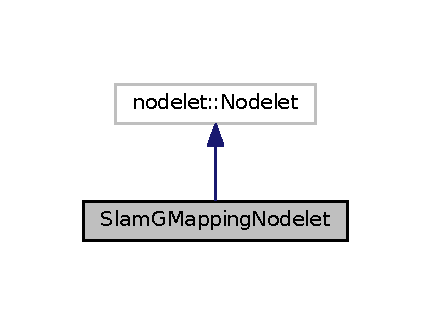
\includegraphics[width=207pt]{classSlamGMappingNodelet__inherit__graph}
\end{center}
\end{figure}


Collaboration diagram for Slam\+G\+Mapping\+Nodelet\+:\nopagebreak
\begin{figure}[H]
\begin{center}
\leavevmode
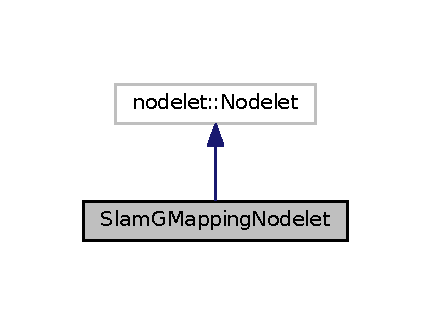
\includegraphics[width=207pt]{classSlamGMappingNodelet__coll__graph}
\end{center}
\end{figure}
\subsection*{Public Member Functions}
\begin{DoxyCompactItemize}
\item 
\hyperlink{classSlamGMappingNodelet_a32123727740dda66cf9f9905dc292015}{Slam\+G\+Mapping\+Nodelet} ()
\item 
\hyperlink{classSlamGMappingNodelet_a194f2f816307faf96427dc77c302c89a}{$\sim$\+Slam\+G\+Mapping\+Nodelet} ()
\item 
virtual void \hyperlink{classSlamGMappingNodelet_afeec962f825e389b6a52cd7f9debf425}{on\+Init} ()
\end{DoxyCompactItemize}


\subsection{Constructor \& Destructor Documentation}
\index{Slam\+G\+Mapping\+Nodelet@{Slam\+G\+Mapping\+Nodelet}!Slam\+G\+Mapping\+Nodelet@{Slam\+G\+Mapping\+Nodelet}}
\index{Slam\+G\+Mapping\+Nodelet@{Slam\+G\+Mapping\+Nodelet}!Slam\+G\+Mapping\+Nodelet@{Slam\+G\+Mapping\+Nodelet}}
\subsubsection[{\texorpdfstring{Slam\+G\+Mapping\+Nodelet()}{SlamGMappingNodelet()}}]{\setlength{\rightskip}{0pt plus 5cm}Slam\+G\+Mapping\+Nodelet\+::\+Slam\+G\+Mapping\+Nodelet (
\begin{DoxyParamCaption}
{}
\end{DoxyParamCaption}
)\hspace{0.3cm}{\ttfamily [inline]}}\hypertarget{classSlamGMappingNodelet_a32123727740dda66cf9f9905dc292015}{}\label{classSlamGMappingNodelet_a32123727740dda66cf9f9905dc292015}
\index{Slam\+G\+Mapping\+Nodelet@{Slam\+G\+Mapping\+Nodelet}!````~Slam\+G\+Mapping\+Nodelet@{$\sim$\+Slam\+G\+Mapping\+Nodelet}}
\index{````~Slam\+G\+Mapping\+Nodelet@{$\sim$\+Slam\+G\+Mapping\+Nodelet}!Slam\+G\+Mapping\+Nodelet@{Slam\+G\+Mapping\+Nodelet}}
\subsubsection[{\texorpdfstring{$\sim$\+Slam\+G\+Mapping\+Nodelet()}{~SlamGMappingNodelet()}}]{\setlength{\rightskip}{0pt plus 5cm}Slam\+G\+Mapping\+Nodelet\+::$\sim$\+Slam\+G\+Mapping\+Nodelet (
\begin{DoxyParamCaption}
{}
\end{DoxyParamCaption}
)\hspace{0.3cm}{\ttfamily [inline]}}\hypertarget{classSlamGMappingNodelet_a194f2f816307faf96427dc77c302c89a}{}\label{classSlamGMappingNodelet_a194f2f816307faf96427dc77c302c89a}


\subsection{Member Function Documentation}
\index{Slam\+G\+Mapping\+Nodelet@{Slam\+G\+Mapping\+Nodelet}!on\+Init@{on\+Init}}
\index{on\+Init@{on\+Init}!Slam\+G\+Mapping\+Nodelet@{Slam\+G\+Mapping\+Nodelet}}
\subsubsection[{\texorpdfstring{on\+Init()}{onInit()}}]{\setlength{\rightskip}{0pt plus 5cm}virtual void Slam\+G\+Mapping\+Nodelet\+::on\+Init (
\begin{DoxyParamCaption}
{}
\end{DoxyParamCaption}
)\hspace{0.3cm}{\ttfamily [inline]}, {\ttfamily [virtual]}}\hypertarget{classSlamGMappingNodelet_afeec962f825e389b6a52cd7f9debf425}{}\label{classSlamGMappingNodelet_afeec962f825e389b6a52cd7f9debf425}


The documentation for this class was generated from the following file\+:\begin{DoxyCompactItemize}
\item 
exp\+\_\+assignment3/src/\hyperlink{nodelet_8cpp}{nodelet.\+cpp}\end{DoxyCompactItemize}

\hypertarget{classBehaviors_1_1Sleep}{}\section{Behaviors.\+Sleep Class Reference}
\label{classBehaviors_1_1Sleep}\index{Behaviors.\+Sleep@{Behaviors.\+Sleep}}


\hyperlink{classBehaviors_1_1Sleep}{Sleep}\+: class that describes the \hyperlink{classBehaviors_1_1Sleep}{Sleep} state.  




Inheritance diagram for Behaviors.\+Sleep\+:\nopagebreak
\begin{figure}[H]
\begin{center}
\leavevmode
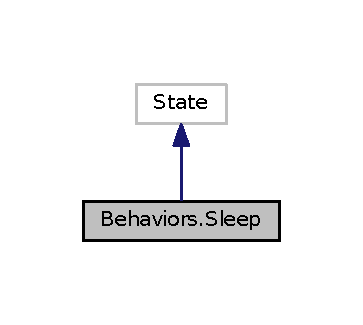
\includegraphics[width=174pt]{classBehaviors_1_1Sleep__inherit__graph}
\end{center}
\end{figure}


Collaboration diagram for Behaviors.\+Sleep\+:\nopagebreak
\begin{figure}[H]
\begin{center}
\leavevmode
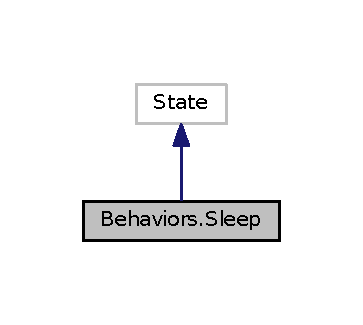
\includegraphics[width=174pt]{classBehaviors_1_1Sleep__coll__graph}
\end{center}
\end{figure}
\subsection*{Public Member Functions}
\begin{DoxyCompactItemize}
\item 
def \hyperlink{classBehaviors_1_1Sleep_accfb4124bccdbacf41004911ab15b447}{\+\_\+\+\_\+init\+\_\+\+\_\+} (self)
\item 
def \hyperlink{classBehaviors_1_1Sleep_ae2eb72a6c74a0c9154e7917550fafae4}{execute} (self, userdata)
\end{DoxyCompactItemize}


\subsection{Detailed Description}
\hyperlink{classBehaviors_1_1Sleep}{Sleep}\+: class that describes the \hyperlink{classBehaviors_1_1Sleep}{Sleep} state. 

\subsection{Constructor \& Destructor Documentation}
\index{Behaviors\+::\+Sleep@{Behaviors\+::\+Sleep}!\+\_\+\+\_\+init\+\_\+\+\_\+@{\+\_\+\+\_\+init\+\_\+\+\_\+}}
\index{\+\_\+\+\_\+init\+\_\+\+\_\+@{\+\_\+\+\_\+init\+\_\+\+\_\+}!Behaviors\+::\+Sleep@{Behaviors\+::\+Sleep}}
\subsubsection[{\texorpdfstring{\+\_\+\+\_\+init\+\_\+\+\_\+(self)}{__init__(self)}}]{\setlength{\rightskip}{0pt plus 5cm}def Behaviors.\+Sleep.\+\_\+\+\_\+init\+\_\+\+\_\+ (
\begin{DoxyParamCaption}
\item[{}]{self}
\end{DoxyParamCaption}
)}\hypertarget{classBehaviors_1_1Sleep_accfb4124bccdbacf41004911ab15b447}{}\label{classBehaviors_1_1Sleep_accfb4124bccdbacf41004911ab15b447}


\subsection{Member Function Documentation}
\index{Behaviors\+::\+Sleep@{Behaviors\+::\+Sleep}!execute@{execute}}
\index{execute@{execute}!Behaviors\+::\+Sleep@{Behaviors\+::\+Sleep}}
\subsubsection[{\texorpdfstring{execute(self, userdata)}{execute(self, userdata)}}]{\setlength{\rightskip}{0pt plus 5cm}def Behaviors.\+Sleep.\+execute (
\begin{DoxyParamCaption}
\item[{}]{self, }
\item[{}]{userdata}
\end{DoxyParamCaption}
)}\hypertarget{classBehaviors_1_1Sleep_ae2eb72a6c74a0c9154e7917550fafae4}{}\label{classBehaviors_1_1Sleep_ae2eb72a6c74a0c9154e7917550fafae4}


The documentation for this class was generated from the following file\+:\begin{DoxyCompactItemize}
\item 
exp\+\_\+assignment3/scripts/\hyperlink{Behaviors_8py}{Behaviors.\+py}\end{DoxyCompactItemize}

\hypertarget{classBehaviors_1_1Track}{}\section{Behaviors.\+Track Class Reference}
\label{classBehaviors_1_1Track}\index{Behaviors.\+Track@{Behaviors.\+Track}}


\hyperlink{classBehaviors_1_1Track}{Track}\+: class that describes the \hyperlink{classBehaviors_1_1Track}{Track} state.  




Inheritance diagram for Behaviors.\+Track\+:\nopagebreak
\begin{figure}[H]
\begin{center}
\leavevmode
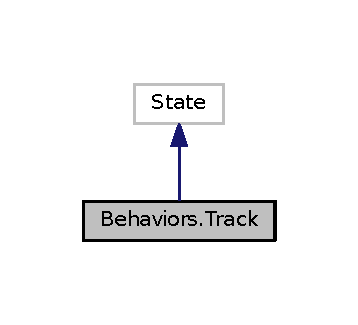
\includegraphics[width=172pt]{classBehaviors_1_1Track__inherit__graph}
\end{center}
\end{figure}


Collaboration diagram for Behaviors.\+Track\+:\nopagebreak
\begin{figure}[H]
\begin{center}
\leavevmode
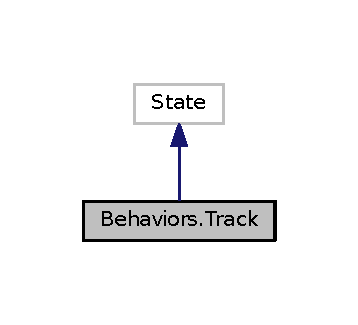
\includegraphics[width=172pt]{classBehaviors_1_1Track__coll__graph}
\end{center}
\end{figure}
\subsection*{Public Member Functions}
\begin{DoxyCompactItemize}
\item 
def \hyperlink{classBehaviors_1_1Track_ad4b822d13b3152463dfae09b7857cafe}{\+\_\+\+\_\+init\+\_\+\+\_\+} (self)
\item 
def \hyperlink{classBehaviors_1_1Track_a35b652d080f4b24379d06d0875c60658}{execute} (self, userdata)
\end{DoxyCompactItemize}


\subsection{Detailed Description}
\hyperlink{classBehaviors_1_1Track}{Track}\+: class that describes the \hyperlink{classBehaviors_1_1Track}{Track} state. 

\subsection{Constructor \& Destructor Documentation}
\index{Behaviors\+::\+Track@{Behaviors\+::\+Track}!\+\_\+\+\_\+init\+\_\+\+\_\+@{\+\_\+\+\_\+init\+\_\+\+\_\+}}
\index{\+\_\+\+\_\+init\+\_\+\+\_\+@{\+\_\+\+\_\+init\+\_\+\+\_\+}!Behaviors\+::\+Track@{Behaviors\+::\+Track}}
\subsubsection[{\texorpdfstring{\+\_\+\+\_\+init\+\_\+\+\_\+(self)}{__init__(self)}}]{\setlength{\rightskip}{0pt plus 5cm}def Behaviors.\+Track.\+\_\+\+\_\+init\+\_\+\+\_\+ (
\begin{DoxyParamCaption}
\item[{}]{self}
\end{DoxyParamCaption}
)}\hypertarget{classBehaviors_1_1Track_ad4b822d13b3152463dfae09b7857cafe}{}\label{classBehaviors_1_1Track_ad4b822d13b3152463dfae09b7857cafe}


\subsection{Member Function Documentation}
\index{Behaviors\+::\+Track@{Behaviors\+::\+Track}!execute@{execute}}
\index{execute@{execute}!Behaviors\+::\+Track@{Behaviors\+::\+Track}}
\subsubsection[{\texorpdfstring{execute(self, userdata)}{execute(self, userdata)}}]{\setlength{\rightskip}{0pt plus 5cm}def Behaviors.\+Track.\+execute (
\begin{DoxyParamCaption}
\item[{}]{self, }
\item[{}]{userdata}
\end{DoxyParamCaption}
)}\hypertarget{classBehaviors_1_1Track_a35b652d080f4b24379d06d0875c60658}{}\label{classBehaviors_1_1Track_a35b652d080f4b24379d06d0875c60658}


The documentation for this class was generated from the following file\+:\begin{DoxyCompactItemize}
\item 
exp\+\_\+assignment3/scripts/\hyperlink{Behaviors_8py}{Behaviors.\+py}\end{DoxyCompactItemize}

\chapter{File Documentation}
\hypertarget{exp__assignment3_2CMakeLists_8txt}{}\section{exp\+\_\+assignment3/\+C\+Make\+Lists.txt File Reference}
\label{exp__assignment3_2CMakeLists_8txt}\index{exp\+\_\+assignment3/\+C\+Make\+Lists.\+txt@{exp\+\_\+assignment3/\+C\+Make\+Lists.\+txt}}

\hypertarget{m-explore_2explore_2CMakeLists_8txt}{}\section{m-\/explore/explore/\+C\+Make\+Lists.txt File Reference}
\label{m-explore_2explore_2CMakeLists_8txt}\index{m-\/explore/explore/\+C\+Make\+Lists.\+txt@{m-\/explore/explore/\+C\+Make\+Lists.\+txt}}

\hypertarget{motion__plan_2CMakeLists_8txt}{}\section{motion\+\_\+plan/\+C\+Make\+Lists.txt File Reference}
\label{motion__plan_2CMakeLists_8txt}\index{motion\+\_\+plan/\+C\+Make\+Lists.\+txt@{motion\+\_\+plan/\+C\+Make\+Lists.\+txt}}

\hypertarget{slam__gmapping_2slam__gmapping_2CMakeLists_8txt}{}\section{slam\+\_\+gmapping/slam\+\_\+gmapping/\+C\+Make\+Lists.txt File Reference}
\label{slam__gmapping_2slam__gmapping_2CMakeLists_8txt}\index{slam\+\_\+gmapping/slam\+\_\+gmapping/\+C\+Make\+Lists.\+txt@{slam\+\_\+gmapping/slam\+\_\+gmapping/\+C\+Make\+Lists.\+txt}}

\hypertarget{Behaviors_8py}{}\section{exp\+\_\+assignment3/scripts/\+Behaviors.py File Reference}
\label{Behaviors_8py}\index{exp\+\_\+assignment3/scripts/\+Behaviors.\+py@{exp\+\_\+assignment3/scripts/\+Behaviors.\+py}}
\subsection*{Classes}
\begin{DoxyCompactItemize}
\item 
class \hyperlink{classBehaviors_1_1Sleep}{Behaviors.\+Sleep}
\begin{DoxyCompactList}\small\item\em \hyperlink{classBehaviors_1_1Sleep}{Sleep}\+: class that describes the \hyperlink{classBehaviors_1_1Sleep}{Sleep} state. \end{DoxyCompactList}\item 
class \hyperlink{classBehaviors_1_1Normal}{Behaviors.\+Normal}
\begin{DoxyCompactList}\small\item\em \hyperlink{classBehaviors_1_1Normal}{Normal}\+: class that describes the \hyperlink{classBehaviors_1_1Normal}{Normal} state. \end{DoxyCompactList}\item 
class \hyperlink{classBehaviors_1_1Play}{Behaviors.\+Play}
\begin{DoxyCompactList}\small\item\em \hyperlink{classBehaviors_1_1Play}{Play}\+: class that describes the \hyperlink{classBehaviors_1_1Play}{Play} state. \end{DoxyCompactList}\item 
class \hyperlink{classBehaviors_1_1Find}{Behaviors.\+Find}
\begin{DoxyCompactList}\small\item\em \hyperlink{classBehaviors_1_1Find}{Find}\+: class that describes the \hyperlink{classBehaviors_1_1Find}{Find} state. \end{DoxyCompactList}\item 
class \hyperlink{classBehaviors_1_1Track}{Behaviors.\+Track}
\begin{DoxyCompactList}\small\item\em \hyperlink{classBehaviors_1_1Track}{Track}\+: class that describes the \hyperlink{classBehaviors_1_1Track}{Track} state. \end{DoxyCompactList}\item 
class \hyperlink{classBehaviors_1_1Recovery}{Behaviors.\+Recovery}
\begin{DoxyCompactList}\small\item\em \hyperlink{classBehaviors_1_1Recovery}{Recovery}\+: class that describes the \hyperlink{classBehaviors_1_1Recovery}{Recovery} state. \end{DoxyCompactList}\end{DoxyCompactItemize}
\subsection*{Namespaces}
\begin{DoxyCompactItemize}
\item 
 \hyperlink{namespaceBehaviors}{Behaviors}
\end{DoxyCompactItemize}
\subsection*{Functions}
\begin{DoxyCompactItemize}
\item 
def \hyperlink{namespaceBehaviors_ab583cdd0339b053bae9c90edfa3ac54e}{Behaviors.\+odom\+\_\+callback} (ros\+\_\+data)
\begin{DoxyCompactList}\small\item\em Callback to retreive the odometry. \end{DoxyCompactList}\item 
def \hyperlink{namespaceBehaviors_a90e1204c5a8da2ddecfa10a3341445a2}{Behaviors.\+status\+\_\+callback} (rosdata)
\begin{DoxyCompactList}\small\item\em Callback to retreive the status of the action server of the motion. \end{DoxyCompactList}\item 
def \hyperlink{namespaceBehaviors_a28e96174292117b887235e69fca82ca5}{Behaviors.\+recovery\+\_\+callback} (rosdata)
\begin{DoxyCompactList}\small\item\em Function to set the recovery state if a signal is sent from R\+V\+IZ. \end{DoxyCompactList}\item 
def \hyperlink{namespaceBehaviors_a7cc21a6fee5a1d2a1139df067ef86299}{Behaviors.\+cancel} ()
\begin{DoxyCompactList}\small\item\em Function to cancel the current move\+\_\+base goal. \end{DoxyCompactList}\item 
def \hyperlink{namespaceBehaviors_a7cc66788be2327e620e1093febba1bcd}{Behaviors.\+set\+Position} (x, y, theta)
\begin{DoxyCompactList}\small\item\em Function to assign the robot position via the action server. \end{DoxyCompactList}\item 
def \hyperlink{namespaceBehaviors_a8c0daf846b80162d86c3e45a605579be}{Behaviors.\+roam} ()
\begin{DoxyCompactList}\small\item\em roam\+: function to simulate the roaming behaviour of normal \end{DoxyCompactList}\end{DoxyCompactItemize}
\subsection*{Variables}
\begin{DoxyCompactItemize}
\item 
\hyperlink{namespaceBehaviors_a480c99d5a0219bba3f364d4022512bda}{Behaviors.\+client} = actionlib.\+Simple\+Action\+Client(\textquotesingle{}/move\+\_\+base\textquotesingle{},Move\+Base\+Action)
\begin{DoxyCompactList}\small\item\em action service client definition \end{DoxyCompactList}\item 
int \hyperlink{namespaceBehaviors_a7ea0e9c25ae327630daf14912540597f}{Behaviors.\+status} = 0
\begin{DoxyCompactList}\small\item\em Variables declaration. \end{DoxyCompactList}\item 
list \hyperlink{namespaceBehaviors_a7fda1c0de76b996b876dad16ed5c7cf5}{Behaviors.\+robot\+\_\+state} = \mbox{[}0,0,0\mbox{]}
\item 
int \hyperlink{namespaceBehaviors_a2de241e90497b66cefc28211136d938b}{Behaviors.\+prev\+\_\+state} = 0
\item 
\hyperlink{namespaceBehaviors_a458a2eb75561d95075537ee82dea289c}{Behaviors.\+Odometry}
\begin{DoxyCompactList}\small\item\em Subscribers definitions. \end{DoxyCompactList}\item 
\hyperlink{namespaceBehaviors_a53b9b8729733e5fde4c917a2068d6c92}{Behaviors.\+odom\+\_\+callback}
\item 
\hyperlink{namespaceBehaviors_a182345f6e56bfb62f2fe95e488624da4}{Behaviors.\+queue\+\_\+size}
\item 
\hyperlink{namespaceBehaviors_a56b79b8920b23a79eb3459479c6342eb}{Behaviors.\+vel\+\_\+pub}
\item 
\hyperlink{namespaceBehaviors_ad0289fe265166267c21567f44c2ecba7}{Behaviors.\+goal\+\_\+pub} = rospy.\+Publisher(\char`\"{}/move\+\_\+base\+\_\+simple/goal\char`\"{}, Pose\+Stamped,queue\+\_\+size=1)
\item 
\hyperlink{namespaceBehaviors_a53817d008ea8a92222a7b07415fd0e7e}{Behaviors.\+Goal\+Status\+Array}
\item 
\hyperlink{namespaceBehaviors_a151c2aa7ae62991aea8bc9a08e0e641b}{Behaviors.\+status\+\_\+callback}
\item 
\hyperlink{namespaceBehaviors_a2fecce674af17c4fbb23fc449c84f934}{Behaviors.\+cancel\+\_\+pub} = rospy.\+Publisher(\char`\"{}/move\+\_\+base/cancel\char`\"{}, Goal\+ID,queue\+\_\+size=1)
\item 
\hyperlink{namespaceBehaviors_a46e25ae172a62cf80114356ad513b371}{Behaviors.\+Pose\+Stamped}
\item 
\hyperlink{namespaceBehaviors_a58f5bdd371d18a7f2a82d97b0db5a536}{Behaviors.\+recovery\+\_\+callback}
\item 
\hyperlink{namespaceBehaviors_a8d923766f9ce0a45edee2abc4ddd7dfd}{Behaviors.\+sm\+\_\+s\+\_\+a} = smach.\+State\+Machine(outcomes=\mbox{[}\textquotesingle{}outcome6\textquotesingle{}\mbox{]})
\begin{DoxyCompactList}\small\item\em Main function declaration. \end{DoxyCompactList}\item 
\hyperlink{namespaceBehaviors_a37367cb6a42ce97b27fc6b024c7fe079}{Behaviors.\+transitions}
\begin{DoxyCompactList}\small\item\em Open the container. \end{DoxyCompactList}\item 
\hyperlink{namespaceBehaviors_ae349e339b61a19499bcd34baefbd77ba}{Behaviors.\+outcome} = sm\+\_\+s\+\_\+a.\+execute()
\begin{DoxyCompactList}\small\item\em Execute S\+M\+A\+CH plan. \end{DoxyCompactList}\end{DoxyCompactItemize}

\hypertarget{bug__m_8py}{}\section{exp\+\_\+assignment3/scripts/bug\+\_\+m.py File Reference}
\label{bug__m_8py}\index{exp\+\_\+assignment3/scripts/bug\+\_\+m.\+py@{exp\+\_\+assignment3/scripts/bug\+\_\+m.\+py}}
\subsection*{Namespaces}
\begin{DoxyCompactItemize}
\item 
 \hyperlink{namespacebug__m}{bug\+\_\+m}
\end{DoxyCompactItemize}
\subsection*{Functions}
\begin{DoxyCompactItemize}
\item 
def \hyperlink{namespacebug__m_a27cfd2a326148157d3e5e0affbe763f3}{bug\+\_\+m.\+clbk\+\_\+odom} (msg)
\item 
def \hyperlink{namespacebug__m_a6ab3d92b5b6ea12eaa52bf21cfa111f1}{bug\+\_\+m.\+clbk\+\_\+laser} (msg)
\item 
def \hyperlink{namespacebug__m_aca19305feae5c5489e7452e921fcbd9c}{bug\+\_\+m.\+change\+\_\+state} (state)
\item 
def \hyperlink{namespacebug__m_a6547c5ebcd1d3aa3e104a5b573e47862}{bug\+\_\+m.\+normalize\+\_\+angle} (angle)
\item 
def \hyperlink{namespacebug__m_a357589ad533151302b9fa9a893833382}{bug\+\_\+m.\+main} ()
\end{DoxyCompactItemize}
\subsection*{Variables}
\begin{DoxyCompactItemize}
\item 
\hyperlink{namespacebug__m_adc14150838edf40c8028207cd6bb2082}{bug\+\_\+m.\+pub} = None
\item 
\hyperlink{namespacebug__m_abd32bbd25b55f71e56505e72ba56c2f6}{bug\+\_\+m.\+srv\+\_\+client\+\_\+go\+\_\+to\+\_\+point\+\_\+} = None
\item 
\hyperlink{namespacebug__m_af40e8063430e5b54ef2f3f8368338744}{bug\+\_\+m.\+srv\+\_\+client\+\_\+wall\+\_\+follower\+\_\+} = None
\item 
int \hyperlink{namespacebug__m_a8b5b5c9259592b8efd526c5adb95d95b}{bug\+\_\+m.\+yaw\+\_\+} = 0
\item 
int \hyperlink{namespacebug__m_a23e5e76f14d9d0d139767cb229a53dda}{bug\+\_\+m.\+yaw\+\_\+error\+\_\+allowed\+\_\+} = 5
\item 
\hyperlink{namespacebug__m_ab108d02234aa3ec58605b9f6980ec090}{bug\+\_\+m.\+position\+\_\+} = Point()
\item 
\hyperlink{namespacebug__m_a8fb60e35f164091fe3355d3a0bce95af}{bug\+\_\+m.\+desired\+\_\+position\+\_\+} = Point()
\item 
\hyperlink{namespacebug__m_af10f89c7f929c9babce108f5d7382996}{bug\+\_\+m.\+x}
\item 
\hyperlink{namespacebug__m_ab8596d2ae799585b0d89152b55891aa8}{bug\+\_\+m.\+y}
\item 
\hyperlink{namespacebug__m_afbb54887da57b97920c8d36c6daed1fc}{bug\+\_\+m.\+z}
\item 
\hyperlink{namespacebug__m_ac9d4d95c034fca5a2b5d08ea845bbfcb}{bug\+\_\+m.\+regions\+\_\+} = None
\item 
list \hyperlink{namespacebug__m_ae70f71d3816862f72790fae7bfaa543b}{bug\+\_\+m.\+state\+\_\+desc\+\_\+} = \mbox{[}\textquotesingle{}Go \hyperlink{wiki__doc_8txt_a59f010b39e38734a32109cf8c8310f81}{to} point\textquotesingle{}, \textquotesingle{}wall following\textquotesingle{}, \textquotesingle{}target reached\textquotesingle{}\mbox{]}
\item 
int \hyperlink{namespacebug__m_a79dc362dff5bef439beacdd5c0c3b2f1}{bug\+\_\+m.\+state\+\_\+} = 0
\end{DoxyCompactItemize}

\hypertarget{exp__assignment3_2scripts_2go__to__point__action_8py}{}\section{exp\+\_\+assignment3/scripts/go\+\_\+to\+\_\+point\+\_\+action.py File Reference}
\label{exp__assignment3_2scripts_2go__to__point__action_8py}\index{exp\+\_\+assignment3/scripts/go\+\_\+to\+\_\+point\+\_\+action.\+py@{exp\+\_\+assignment3/scripts/go\+\_\+to\+\_\+point\+\_\+action.\+py}}
\subsection*{Namespaces}
\begin{DoxyCompactItemize}
\item 
 \hyperlink{namespacego__to__point__action}{go\+\_\+to\+\_\+point\+\_\+action}
\end{DoxyCompactItemize}
\subsection*{Functions}
\begin{DoxyCompactItemize}
\item 
def \hyperlink{namespacego__to__point__action_a071343dec01124a125b208f881e350ff}{go\+\_\+to\+\_\+point\+\_\+action.\+clbk\+\_\+odom} (msg)
\begin{DoxyCompactList}\small\item\em callbacks \end{DoxyCompactList}\item 
def \hyperlink{namespacego__to__point__action_a228c91a7de8ba144bebc1621674878da}{go\+\_\+to\+\_\+point\+\_\+action.\+change\+\_\+state} (state)
\begin{DoxyCompactList}\small\item\em change state \end{DoxyCompactList}\item 
def \hyperlink{namespacego__to__point__action_a595bc16b669d1573a921f2fc42d61961}{go\+\_\+to\+\_\+point\+\_\+action.\+normalize\+\_\+angle} (angle)
\item 
def \hyperlink{namespacego__to__point__action_a4a5f8180b546da8703ac2dddf1a70e5d}{go\+\_\+to\+\_\+point\+\_\+action.\+fix\+\_\+yaw} (des\+\_\+pos)
\item 
def \hyperlink{namespacego__to__point__action_a15dbc5b1176cdaf104c33ce8eb7e6103}{go\+\_\+to\+\_\+point\+\_\+action.\+go\+\_\+straight\+\_\+ahead} (des\+\_\+pos)
\begin{DoxyCompactList}\small\item\em function to go straight ahead \end{DoxyCompactList}\item 
def \hyperlink{namespacego__to__point__action_a99cfe9dae88227814c5387387fe794c5}{go\+\_\+to\+\_\+point\+\_\+action.\+done} ()
\begin{DoxyCompactList}\small\item\em Function to terminate the control when target is achieved. \end{DoxyCompactList}\item 
def \hyperlink{namespacego__to__point__action_a5bba71b4503c075067b2bbfcdf64556e}{go\+\_\+to\+\_\+point\+\_\+action.\+planning} (goal)
\begin{DoxyCompactList}\small\item\em Function to plan the control to reach the target. \end{DoxyCompactList}\item 
def \hyperlink{namespacego__to__point__action_ad5e10fe384fcab186e405aac29aece7b}{go\+\_\+to\+\_\+point\+\_\+action.\+main} ()
\begin{DoxyCompactList}\small\item\em main function \end{DoxyCompactList}\end{DoxyCompactItemize}
\subsection*{Variables}
\begin{DoxyCompactItemize}
\item 
\hyperlink{namespacego__to__point__action_a4aafc5721803ca4d208e9e0a686f8e65}{go\+\_\+to\+\_\+point\+\_\+action.\+position\+\_\+} = Point()
\begin{DoxyCompactList}\small\item\em robot state variables \end{DoxyCompactList}\item 
\hyperlink{namespacego__to__point__action_ac843a0e43a672ed873017530721ce2d9}{go\+\_\+to\+\_\+point\+\_\+action.\+pose\+\_\+} = Pose()
\item 
int \hyperlink{namespacego__to__point__action_a880fb089b41232984ae49355b6f46a39}{go\+\_\+to\+\_\+point\+\_\+action.\+yaw\+\_\+} = 0
\item 
int \hyperlink{namespacego__to__point__action_aadf404dc66c95a101e7e05dfafd92c3d}{go\+\_\+to\+\_\+point\+\_\+action.\+state\+\_\+} = 0
\begin{DoxyCompactList}\small\item\em machine state \end{DoxyCompactList}\item 
\hyperlink{namespacego__to__point__action_a57e8782cf693baab2ca4390e2e917155}{go\+\_\+to\+\_\+point\+\_\+action.\+desired\+\_\+position\+\_\+} = Point()
\begin{DoxyCompactList}\small\item\em goal \end{DoxyCompactList}\item 
\hyperlink{namespacego__to__point__action_a8848541ff0d9e1607e1d715de007aa03}{go\+\_\+to\+\_\+point\+\_\+action.\+z}
\item 
int \hyperlink{namespacego__to__point__action_a914253ff638fc05f3f0fd3d9536503c2}{go\+\_\+to\+\_\+point\+\_\+action.\+yaw\+\_\+precision\+\_\+} = math.\+pi/9
\begin{DoxyCompactList}\small\item\em parameters \end{DoxyCompactList}\item 
int \hyperlink{namespacego__to__point__action_a65f4bbc971a7e33d9441aa79dcbfa1ae}{go\+\_\+to\+\_\+point\+\_\+action.\+yaw\+\_\+precision\+\_\+2\+\_\+} = math.\+pi/90
\begin{DoxyCompactList}\small\item\em +/-\/ 20 degree allowed \end{DoxyCompactList}\item 
float \hyperlink{namespacego__to__point__action_a2b67a832bde842bf565341c5fc606f81}{go\+\_\+to\+\_\+point\+\_\+action.\+dist\+\_\+precision\+\_\+} = 0.\+1
\begin{DoxyCompactList}\small\item\em +/-\/ 2 degree allowed \end{DoxyCompactList}\item 
float \hyperlink{namespacego__to__point__action_a9f06acd5d2562909e122242d328755df}{go\+\_\+to\+\_\+point\+\_\+action.\+kp\+\_\+a} = 3.\+0
\item 
float \hyperlink{namespacego__to__point__action_a34be7fb79cc4f03e9b8671df19275132}{go\+\_\+to\+\_\+point\+\_\+action.\+kp\+\_\+d} = 0.\+2
\begin{DoxyCompactList}\small\item\em In R\+OS Noetic, it may be necessary to change the sign of this proportional controller. \end{DoxyCompactList}\item 
float \hyperlink{namespacego__to__point__action_a2c03541662b19da8a707e89f121e25a5}{go\+\_\+to\+\_\+point\+\_\+action.\+ub\+\_\+a} = 0.\+9
\item 
float \hyperlink{namespacego__to__point__action_ac93d2080cb249db79a1bba87a42c1a44}{go\+\_\+to\+\_\+point\+\_\+action.\+lb\+\_\+a} = -\/0.\+9
\item 
float \hyperlink{namespacego__to__point__action_a6450364749bdc94394b2251c68e2ceee}{go\+\_\+to\+\_\+point\+\_\+action.\+ub\+\_\+d} = 0.\+6
\item 
\hyperlink{namespacego__to__point__action_a3e555da71db618b9165bb58fe9ef160e}{go\+\_\+to\+\_\+point\+\_\+action.\+pub} = None
\begin{DoxyCompactList}\small\item\em publisher \end{DoxyCompactList}\item 
\hyperlink{namespacego__to__point__action_a3994b1577d1a499ce8c7352036ee6486}{go\+\_\+to\+\_\+point\+\_\+action.\+act\+\_\+s} = None
\begin{DoxyCompactList}\small\item\em action\+\_\+server \end{DoxyCompactList}\end{DoxyCompactItemize}

\hypertarget{motion__plan_2scripts_2go__to__point__action_8py}{}\section{motion\+\_\+plan/scripts/go\+\_\+to\+\_\+point\+\_\+action.py File Reference}
\label{motion__plan_2scripts_2go__to__point__action_8py}\index{motion\+\_\+plan/scripts/go\+\_\+to\+\_\+point\+\_\+action.\+py@{motion\+\_\+plan/scripts/go\+\_\+to\+\_\+point\+\_\+action.\+py}}
\subsection*{Namespaces}
\begin{DoxyCompactItemize}
\item 
 \hyperlink{namespacego__to__point__action}{go\+\_\+to\+\_\+point\+\_\+action}
\end{DoxyCompactItemize}
\subsection*{Functions}
\begin{DoxyCompactItemize}
\item 
def \hyperlink{namespacego__to__point__action_a071343dec01124a125b208f881e350ff}{go\+\_\+to\+\_\+point\+\_\+action.\+clbk\+\_\+odom} (msg)
\begin{DoxyCompactList}\small\item\em callbacks \end{DoxyCompactList}\item 
def \hyperlink{namespacego__to__point__action_a228c91a7de8ba144bebc1621674878da}{go\+\_\+to\+\_\+point\+\_\+action.\+change\+\_\+state} (state)
\begin{DoxyCompactList}\small\item\em change state \end{DoxyCompactList}\item 
def \hyperlink{namespacego__to__point__action_a595bc16b669d1573a921f2fc42d61961}{go\+\_\+to\+\_\+point\+\_\+action.\+normalize\+\_\+angle} (angle)
\item 
def \hyperlink{namespacego__to__point__action_a4a5f8180b546da8703ac2dddf1a70e5d}{go\+\_\+to\+\_\+point\+\_\+action.\+fix\+\_\+yaw} (des\+\_\+pos)
\item 
def \hyperlink{namespacego__to__point__action_a15dbc5b1176cdaf104c33ce8eb7e6103}{go\+\_\+to\+\_\+point\+\_\+action.\+go\+\_\+straight\+\_\+ahead} (des\+\_\+pos)
\begin{DoxyCompactList}\small\item\em function to go straight ahead \end{DoxyCompactList}\item 
def \hyperlink{namespacego__to__point__action_a99cfe9dae88227814c5387387fe794c5}{go\+\_\+to\+\_\+point\+\_\+action.\+done} ()
\begin{DoxyCompactList}\small\item\em Function to terminate the control when target is achieved. \end{DoxyCompactList}\item 
def \hyperlink{namespacego__to__point__action_a5bba71b4503c075067b2bbfcdf64556e}{go\+\_\+to\+\_\+point\+\_\+action.\+planning} (goal)
\begin{DoxyCompactList}\small\item\em Function to plan the control to reach the target. \end{DoxyCompactList}\item 
def \hyperlink{namespacego__to__point__action_ad5e10fe384fcab186e405aac29aece7b}{go\+\_\+to\+\_\+point\+\_\+action.\+main} ()
\begin{DoxyCompactList}\small\item\em main function \end{DoxyCompactList}\end{DoxyCompactItemize}

\hypertarget{go__to__point__service__m_8py}{}\section{exp\+\_\+assignment3/scripts/go\+\_\+to\+\_\+point\+\_\+service\+\_\+m.py File Reference}
\label{go__to__point__service__m_8py}\index{exp\+\_\+assignment3/scripts/go\+\_\+to\+\_\+point\+\_\+service\+\_\+m.\+py@{exp\+\_\+assignment3/scripts/go\+\_\+to\+\_\+point\+\_\+service\+\_\+m.\+py}}
\subsection*{Namespaces}
\begin{DoxyCompactItemize}
\item 
 \hyperlink{namespacego__to__point__service__m}{go\+\_\+to\+\_\+point\+\_\+service\+\_\+m}
\end{DoxyCompactItemize}
\subsection*{Functions}
\begin{DoxyCompactItemize}
\item 
def \hyperlink{namespacego__to__point__service__m_a5aa5049687ed47c4e5e85903267700ee}{go\+\_\+to\+\_\+point\+\_\+service\+\_\+m.\+go\+\_\+to\+\_\+point\+\_\+switch} (req)
\item 
def \hyperlink{namespacego__to__point__service__m_a379907ef466483603becace59e6f973b}{go\+\_\+to\+\_\+point\+\_\+service\+\_\+m.\+clbk\+\_\+odom} (msg)
\item 
def \hyperlink{namespacego__to__point__service__m_a40af22e9a0b3ac0544d0c08b246e6436}{go\+\_\+to\+\_\+point\+\_\+service\+\_\+m.\+change\+\_\+state} (state)
\item 
def \hyperlink{namespacego__to__point__service__m_a9016b8d25737fe805f75d9db52ff4680}{go\+\_\+to\+\_\+point\+\_\+service\+\_\+m.\+normalize\+\_\+angle} (angle)
\item 
def \hyperlink{namespacego__to__point__service__m_a45b937484f29d60d6578dd670f07f241}{go\+\_\+to\+\_\+point\+\_\+service\+\_\+m.\+fix\+\_\+yaw} (des\+\_\+pos)
\item 
def \hyperlink{namespacego__to__point__service__m_aa0efa6e8f30a39de9a6440888882daf1}{go\+\_\+to\+\_\+point\+\_\+service\+\_\+m.\+go\+\_\+straight\+\_\+ahead} (des\+\_\+pos)
\item 
def \hyperlink{namespacego__to__point__service__m_a22f1876bd87959557a463d43fa521ad3}{go\+\_\+to\+\_\+point\+\_\+service\+\_\+m.\+done} (des\+\_\+pos)
\item 
def \hyperlink{namespacego__to__point__service__m_a294bca40052b9b1c83ddf85a023b276e}{go\+\_\+to\+\_\+point\+\_\+service\+\_\+m.\+main} ()
\end{DoxyCompactItemize}
\subsection*{Variables}
\begin{DoxyCompactItemize}
\item 
bool \hyperlink{namespacego__to__point__service__m_a0a0a9847f2d5f0059f48709cba4df15c}{go\+\_\+to\+\_\+point\+\_\+service\+\_\+m.\+active\+\_\+} = False
\item 
\hyperlink{namespacego__to__point__service__m_abb95705acc8e0b8a82a6fc5d6243bdd8}{go\+\_\+to\+\_\+point\+\_\+service\+\_\+m.\+position\+\_\+} = Point()
\item 
int \hyperlink{namespacego__to__point__service__m_ab1e499009bca0d4c9ea5e8954aa37797}{go\+\_\+to\+\_\+point\+\_\+service\+\_\+m.\+yaw\+\_\+} = 0
\item 
int \hyperlink{namespacego__to__point__service__m_a840bab237e425d4f242bf69afe92f767}{go\+\_\+to\+\_\+point\+\_\+service\+\_\+m.\+state\+\_\+} = 0
\item 
\hyperlink{namespacego__to__point__service__m_a5e4a4244e883c27be9ed897ea5460cc0}{go\+\_\+to\+\_\+point\+\_\+service\+\_\+m.\+desired\+\_\+position\+\_\+} = Point()
\item 
\hyperlink{namespacego__to__point__service__m_a3ec6e272b02c0f40a625358965caf70b}{go\+\_\+to\+\_\+point\+\_\+service\+\_\+m.\+x}
\item 
\hyperlink{namespacego__to__point__service__m_a8a0df04be6cfa44113ee26eefbe11f95}{go\+\_\+to\+\_\+point\+\_\+service\+\_\+m.\+y}
\item 
\hyperlink{namespacego__to__point__service__m_aa0ed9dc81f0153863a2a971384dbcba3}{go\+\_\+to\+\_\+point\+\_\+service\+\_\+m.\+z}
\item 
int \hyperlink{namespacego__to__point__service__m_af47f1354626111fc63115c06276ae41d}{go\+\_\+to\+\_\+point\+\_\+service\+\_\+m.\+yaw\+\_\+precision\+\_\+} = math.\+pi/9
\item 
int \hyperlink{namespacego__to__point__service__m_aa642aefafe9c9c963a86f01c5a256e23}{go\+\_\+to\+\_\+point\+\_\+service\+\_\+m.\+yaw\+\_\+precision\+\_\+2\+\_\+} = math.\+pi/90
\item 
float \hyperlink{namespacego__to__point__service__m_a15a85217148ccc92490d2ec8366dfbd4}{go\+\_\+to\+\_\+point\+\_\+service\+\_\+m.\+dist\+\_\+precision\+\_\+} = 0.\+3
\item 
float \hyperlink{namespacego__to__point__service__m_a7e9c758884ac92bbb820e532fd32abf6}{go\+\_\+to\+\_\+point\+\_\+service\+\_\+m.\+kp\+\_\+a} = 3.\+0
\item 
float \hyperlink{namespacego__to__point__service__m_aa9ffa11cdce18c2942bca64db42cb249}{go\+\_\+to\+\_\+point\+\_\+service\+\_\+m.\+kp\+\_\+d} = 0.\+2
\item 
float \hyperlink{namespacego__to__point__service__m_ac8de1564925338ead12be0a3763b4119}{go\+\_\+to\+\_\+point\+\_\+service\+\_\+m.\+ub\+\_\+a} = 0.\+6
\item 
float \hyperlink{namespacego__to__point__service__m_a66ab9d35823a86f4fee11da3fa6a7157}{go\+\_\+to\+\_\+point\+\_\+service\+\_\+m.\+lb\+\_\+a} = -\/0.\+5
\item 
float \hyperlink{namespacego__to__point__service__m_aba661cc0f865736231acaf5b56101b35}{go\+\_\+to\+\_\+point\+\_\+service\+\_\+m.\+ub\+\_\+d} = 0.\+6
\item 
\hyperlink{namespacego__to__point__service__m_ab9ea0cd28ffda51b5d6f1a436464f861}{go\+\_\+to\+\_\+point\+\_\+service\+\_\+m.\+pub} = None
\end{DoxyCompactItemize}

\hypertarget{Perception_8py}{}\section{exp\+\_\+assignment3/scripts/\+Perception.py File Reference}
\label{Perception_8py}\index{exp\+\_\+assignment3/scripts/\+Perception.\+py@{exp\+\_\+assignment3/scripts/\+Perception.\+py}}
\subsection*{Classes}
\begin{DoxyCompactItemize}
\item 
class \hyperlink{classPerception_1_1image__feature}{Perception.\+image\+\_\+feature}
\begin{DoxyCompactList}\small\item\em C\+L\+A\+SS. \end{DoxyCompactList}\end{DoxyCompactItemize}
\subsection*{Namespaces}
\begin{DoxyCompactItemize}
\item 
 \hyperlink{namespacePerception}{Perception}
\end{DoxyCompactItemize}
\subsection*{Functions}
\begin{DoxyCompactItemize}
\item 
def \hyperlink{namespacePerception_ae23dae157a1ef4e00fb8d4d11ed4cfd7}{Perception.\+rob\+\_\+callback} (ros\+\_\+data)
\begin{DoxyCompactList}\small\item\em C\+A\+L\+L\+B\+A\+C\+KS A\+ND F\+U\+N\+C\+T\+I\+O\+NS. \end{DoxyCompactList}\item 
def \hyperlink{namespacePerception_a34e5d1ea23bca609f6613f955a102c8f}{Perception.\+laser\+\_\+callback} (ros\+\_\+data)
\begin{DoxyCompactList}\small\item\em callback function to read the laser scan \end{DoxyCompactList}\item 
def \hyperlink{namespacePerception_a235ca282efe20cd6f6553cf69dfa3416}{Perception.\+enclosing\+\_\+circle} (cnts)
\begin{DoxyCompactList}\small\item\em find the enclosing circle of the ball in the image \end{DoxyCompactList}\item 
def \hyperlink{namespacePerception_aad4a17a04d9de153f903bec742d3f1c4}{Perception.\+caption} (image\+\_\+np, x, y, radius, center, name)
\begin{DoxyCompactList}\small\item\em Put a caption and an enclosing circle around a perceived ball. \end{DoxyCompactList}\item 
def \hyperlink{namespacePerception_a2fca011fd161b10ca2292edbb9897af5}{Perception.\+take\+\_\+action} (regions)
\begin{DoxyCompactList}\small\item\em action to take to avoid collisions \end{DoxyCompactList}\item 
def \hyperlink{namespacePerception_a9210db14d4f3a53190632b2097f7444c}{Perception.\+clbk\+\_\+laser} (scan, k)
\begin{DoxyCompactList}\small\item\em obstacles region declaration to obstacle avoidance \end{DoxyCompactList}\item 
def \hyperlink{namespacePerception_a4fe5d026a2ef743aa57777be689aeb43}{Perception.\+main} (args)
\begin{DoxyCompactList}\small\item\em M\+A\+IN. \end{DoxyCompactList}\end{DoxyCompactItemize}
\subsection*{Variables}
\begin{DoxyCompactItemize}
\item 
bool \hyperlink{namespacePerception_a45c9a255f6f96422822a1134c6200451}{Perception.\+V\+E\+R\+B\+O\+SE} = False
\item 
int \hyperlink{namespacePerception_a30f922540fc81da4abe1a1cf48cf96ac}{Perception.\+angle} = 0
\begin{DoxyCompactList}\small\item\em V\+A\+R\+I\+A\+B\+L\+ES. \end{DoxyCompactList}\item 
int \hyperlink{namespacePerception_a9f6f9cf6f9b5895bb39924b3682a262b}{Perception.\+threshold} = 10
\begin{DoxyCompactList}\small\item\em Threshold precision. \end{DoxyCompactList}\item 
int \hyperlink{namespacePerception_a25e59ac83c977a1cd1752b677923c0d8}{Perception.\+max\+\_\+rad} = 180
\begin{DoxyCompactList}\small\item\em Dimension of the proximity radius. \end{DoxyCompactList}\item 
int \hyperlink{namespacePerception_a6f826a3f390ba3a185e2aa8a43013701}{Perception.\+rob\+\_\+angle} = 0
\begin{DoxyCompactList}\small\item\em robot angle \end{DoxyCompactList}\item 
int \hyperlink{namespacePerception_ad0534f9c1df13d7a2b48ff2a983f0cc6}{Perception.\+rob\+\_\+vel} = 0
\begin{DoxyCompactList}\small\item\em robot vel \end{DoxyCompactList}\item 
int \hyperlink{namespacePerception_a32c9e49968ea4ea21f1afbe28dc236cc}{Perception.\+max\+\_\+ang} = 0
\begin{DoxyCompactList}\small\item\em maximum and minimum angle of the scan \end{DoxyCompactList}\item 
int \hyperlink{namespacePerception_a0aca0fa8eb3415fe07777168f37774ff}{Perception.\+min\+\_\+ang} = 0
\item 
list \hyperlink{namespacePerception_a649811d3cb5680f5481c7d612e159825}{Perception.\+scans} = \mbox{[}$\,$\mbox{]}
\item 
float \hyperlink{namespacePerception_ac133c0d0f793260fe4d078d02ec777b6}{Perception.\+value\+\_\+min} = 0.\+30
\item 
int \hyperlink{namespacePerception_a47402108dd4d75ac8a27e5d917aa022c}{Perception.\+rob\+\_\+x} = 0
\item 
int \hyperlink{namespacePerception_ace15e3c972e7a909673f2280e02954a5}{Perception.\+rob\+\_\+y} = 0
\item 
int \hyperlink{namespacePerception_ab4a40230ffe1d9f53908c2c5c6fd6ebb}{Perception.\+rob\+\_\+theta} = 0
\item 
int \hyperlink{namespacePerception_ad34a03e4d4afc6f3f824f912c28692ff}{Perception.\+prev\+\_\+state} = 0
\item 
list \hyperlink{namespacePerception_ade020d1959a087b5a07fd0936a5f489d}{Perception.\+names} = \mbox{[}\char`\"{}Entrance\char`\"{},\char`\"{}Living\+\_\+room\char`\"{},\char`\"{}Closet\char`\"{},\char`\"{}Kitchen\char`\"{},\char`\"{}Bathroom\char`\"{},\char`\"{}Bedroom\char`\"{}\mbox{]}
\begin{DoxyCompactList}\small\item\em R\+O\+O\+MS P\+A\+R\+A\+M\+E\+T\+E\+RS. \end{DoxyCompactList}\item 
list \hyperlink{namespacePerception_a4166a4d5dfba1d1c65be4e69bed3a442}{Perception.\+lower} = \mbox{[}100,50,0,25,125,0\mbox{]}
\item 
list \hyperlink{namespacePerception_a0d76072dc5634b931abcd5275677b670}{Perception.\+upper} = \mbox{[}130,70,5,35,150,5\mbox{]}
\item 
list \hyperlink{namespacePerception_a47f799f9c4dfa904981d74938dcd5e49}{Perception.\+checked} = \mbox{[}0\mbox{]}$\ast$len(names)
\item 
int \hyperlink{namespacePerception_a78a55345c0afe004ebc5bd95007dccf0}{Perception.\+active} = 0
\begin{DoxyCompactList}\small\item\em Track activate variable. \end{DoxyCompactList}\item 
list \hyperlink{namespacePerception_a2df199890febf0c129179eacf940dbaa}{Perception.\+seen} = \mbox{[}0\mbox{]}$\ast$len(checked)
\begin{DoxyCompactList}\small\item\em Seen balls. \end{DoxyCompactList}\item 
list \hyperlink{namespacePerception_ae9b407646d9596cc4c837cadcc084168}{Perception.\+cnts} = \mbox{[}None\mbox{]}$\ast$len(seen)
\begin{DoxyCompactList}\small\item\em Contours. \end{DoxyCompactList}\item 
float \hyperlink{namespacePerception_a353d9d2be3d3ef1de098a6dd0354b5fe}{Perception.\+gain1} = 0.\+003
\begin{DoxyCompactList}\small\item\em G\+A\+I\+NS. \end{DoxyCompactList}\item 
float \hyperlink{namespacePerception_a2520defc2fe01293181f48cc9c93d552}{Perception.\+gain2} = 0.\+042
\item 
float \hyperlink{namespacePerception_a229e55dde1fafbfa34e1ed76f9dab9a7}{Perception.\+gain3} = 0.\+0035
\item 
float \hyperlink{namespacePerception_a1149af80a55cce4661c985f8d4ca15ae}{Perception.\+gain4} = 0.\+04
\end{DoxyCompactItemize}

\hypertarget{user__interface_8py}{}\section{exp\+\_\+assignment3/scripts/user\+\_\+interface.py File Reference}
\label{user__interface_8py}\index{exp\+\_\+assignment3/scripts/user\+\_\+interface.\+py@{exp\+\_\+assignment3/scripts/user\+\_\+interface.\+py}}
\subsection*{Namespaces}
\begin{DoxyCompactItemize}
\item 
 \hyperlink{namespaceuser__interface}{user\+\_\+interface}
\end{DoxyCompactItemize}
\subsection*{Functions}
\begin{DoxyCompactItemize}
\item 
def \hyperlink{namespaceuser__interface_ac26bdb296b6776907b72c17ce5a1b24a}{user\+\_\+interface.\+main} ()
\begin{DoxyCompactList}\small\item\em Main body of code. \end{DoxyCompactList}\end{DoxyCompactItemize}
\subsection*{Variables}
\begin{DoxyCompactItemize}
\item 
int \hyperlink{namespaceuser__interface_a97dbaeb7fcda50910c33a1460636019f}{user\+\_\+interface.\+random\+\_\+timer} = 0
\begin{DoxyCompactList}\small\item\em Variable definition. \end{DoxyCompactList}\item 
list \hyperlink{namespaceuser__interface_a85e1f66e836d4199dd7325354493dff7}{user\+\_\+interface.\+names} = \mbox{[}\char`\"{}Entrance\char`\"{},\char`\"{}Living\+\_\+room\char`\"{},\char`\"{}Bedroom\char`\"{},\char`\"{}Bathroom\char`\"{},\char`\"{}Closet\char`\"{},\char`\"{}Kitchen\char`\"{}\mbox{]}
\end{DoxyCompactItemize}

\hypertarget{wall__follow__service__m_8py}{}\section{exp\+\_\+assignment3/scripts/wall\+\_\+follow\+\_\+service\+\_\+m.py File Reference}
\label{wall__follow__service__m_8py}\index{exp\+\_\+assignment3/scripts/wall\+\_\+follow\+\_\+service\+\_\+m.\+py@{exp\+\_\+assignment3/scripts/wall\+\_\+follow\+\_\+service\+\_\+m.\+py}}
\subsection*{Namespaces}
\begin{DoxyCompactItemize}
\item 
 \hyperlink{namespacewall__follow__service__m}{wall\+\_\+follow\+\_\+service\+\_\+m}
\end{DoxyCompactItemize}
\subsection*{Functions}
\begin{DoxyCompactItemize}
\item 
def \hyperlink{namespacewall__follow__service__m_a8367ccc5f1456166406c0d577d019baf}{wall\+\_\+follow\+\_\+service\+\_\+m.\+wall\+\_\+follower\+\_\+switch} (req)
\item 
def \hyperlink{namespacewall__follow__service__m_ab07be9226f1ee837e03f25d282336b09}{wall\+\_\+follow\+\_\+service\+\_\+m.\+clbk\+\_\+laser} (msg)
\item 
def \hyperlink{namespacewall__follow__service__m_ad99900df1d3fa5dd0683d507b2253b17}{wall\+\_\+follow\+\_\+service\+\_\+m.\+change\+\_\+state} (state)
\item 
def \hyperlink{namespacewall__follow__service__m_a027e1db38933af0544136a5c84de5a83}{wall\+\_\+follow\+\_\+service\+\_\+m.\+take\+\_\+action} ()
\item 
def \hyperlink{namespacewall__follow__service__m_ae65476bf2d8bd9007fda22eaea1ed2b1}{wall\+\_\+follow\+\_\+service\+\_\+m.\+find\+\_\+wall} ()
\item 
def \hyperlink{namespacewall__follow__service__m_aa4262b4e6e90a36c0226c9b90ee97d14}{wall\+\_\+follow\+\_\+service\+\_\+m.\+turn\+\_\+left} ()
\item 
def \hyperlink{namespacewall__follow__service__m_a2f9f1202ed1e75ee80471a9dff56fdbe}{wall\+\_\+follow\+\_\+service\+\_\+m.\+follow\+\_\+the\+\_\+wall} ()
\item 
def \hyperlink{namespacewall__follow__service__m_ab4dbc79e32b45a381737fb7b3c126edf}{wall\+\_\+follow\+\_\+service\+\_\+m.\+main} ()
\end{DoxyCompactItemize}
\subsection*{Variables}
\begin{DoxyCompactItemize}
\item 
bool \hyperlink{namespacewall__follow__service__m_ae80ea3e1537280d2311f2fc113a60bc7}{wall\+\_\+follow\+\_\+service\+\_\+m.\+active\+\_\+} = False
\item 
\hyperlink{namespacewall__follow__service__m_aa66ff19a5a11afad8ec15143f733bea2}{wall\+\_\+follow\+\_\+service\+\_\+m.\+pub\+\_\+} = None
\item 
dictionary \hyperlink{namespacewall__follow__service__m_a30a3b79a68496f06646ee64d67423f36}{wall\+\_\+follow\+\_\+service\+\_\+m.\+regions\+\_\+}
\item 
int \hyperlink{namespacewall__follow__service__m_a1f1e8197a7b86b64c5c2c256173e371d}{wall\+\_\+follow\+\_\+service\+\_\+m.\+state\+\_\+} = 0
\item 
dictionary \hyperlink{namespacewall__follow__service__m_a723d03e512b26cc484d9299418b2773d}{wall\+\_\+follow\+\_\+service\+\_\+m.\+state\+\_\+dict\+\_\+}
\end{DoxyCompactItemize}

\hypertarget{main_8cpp}{}\section{exp\+\_\+assignment3/src/main.cpp File Reference}
\label{main_8cpp}\index{exp\+\_\+assignment3/src/main.\+cpp@{exp\+\_\+assignment3/src/main.\+cpp}}
{\ttfamily \#include $<$ros/ros.\+h$>$}\\*
{\ttfamily \#include \char`\"{}slam\+\_\+gmapping.\+h\char`\"{}}\\*
Include dependency graph for main.\+cpp\+:\nopagebreak
\begin{figure}[H]
\begin{center}
\leavevmode
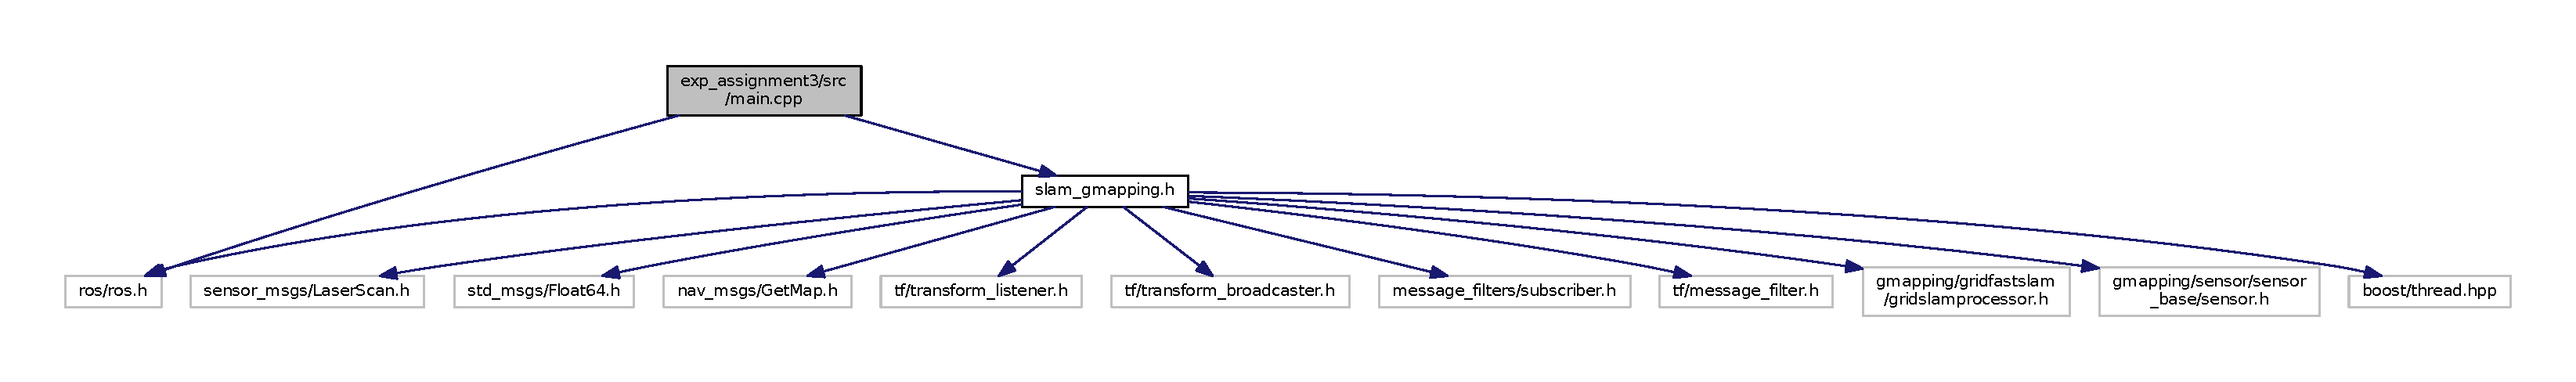
\includegraphics[width=350pt]{main_8cpp__incl}
\end{center}
\end{figure}
\subsection*{Functions}
\begin{DoxyCompactItemize}
\item 
int \hyperlink{main_8cpp_a3c04138a5bfe5d72780bb7e82a18e627}{main} (int argc, char $\ast$$\ast$argv)
\end{DoxyCompactItemize}


\subsection{Function Documentation}
\index{main.\+cpp@{main.\+cpp}!main@{main}}
\index{main@{main}!main.\+cpp@{main.\+cpp}}
\subsubsection[{\texorpdfstring{main(int argc, char $\ast$$\ast$argv)}{main(int argc, char **argv)}}]{\setlength{\rightskip}{0pt plus 5cm}int main (
\begin{DoxyParamCaption}
\item[{int}]{argc, }
\item[{char $\ast$$\ast$}]{argv}
\end{DoxyParamCaption}
)}\hypertarget{main_8cpp_a3c04138a5bfe5d72780bb7e82a18e627}{}\label{main_8cpp_a3c04138a5bfe5d72780bb7e82a18e627}

\hypertarget{nodelet_8cpp}{}\section{exp\+\_\+assignment3/src/nodelet.cpp File Reference}
\label{nodelet_8cpp}\index{exp\+\_\+assignment3/src/nodelet.\+cpp@{exp\+\_\+assignment3/src/nodelet.\+cpp}}
{\ttfamily \#include $<$ros/ros.\+h$>$}\\*
{\ttfamily \#include $<$nodelet/nodelet.\+h$>$}\\*
{\ttfamily \#include $<$pluginlib/class\+\_\+list\+\_\+macros.\+h$>$}\\*
{\ttfamily \#include \char`\"{}slam\+\_\+gmapping.\+h\char`\"{}}\\*
Include dependency graph for nodelet.\+cpp\+:\nopagebreak
\begin{figure}[H]
\begin{center}
\leavevmode
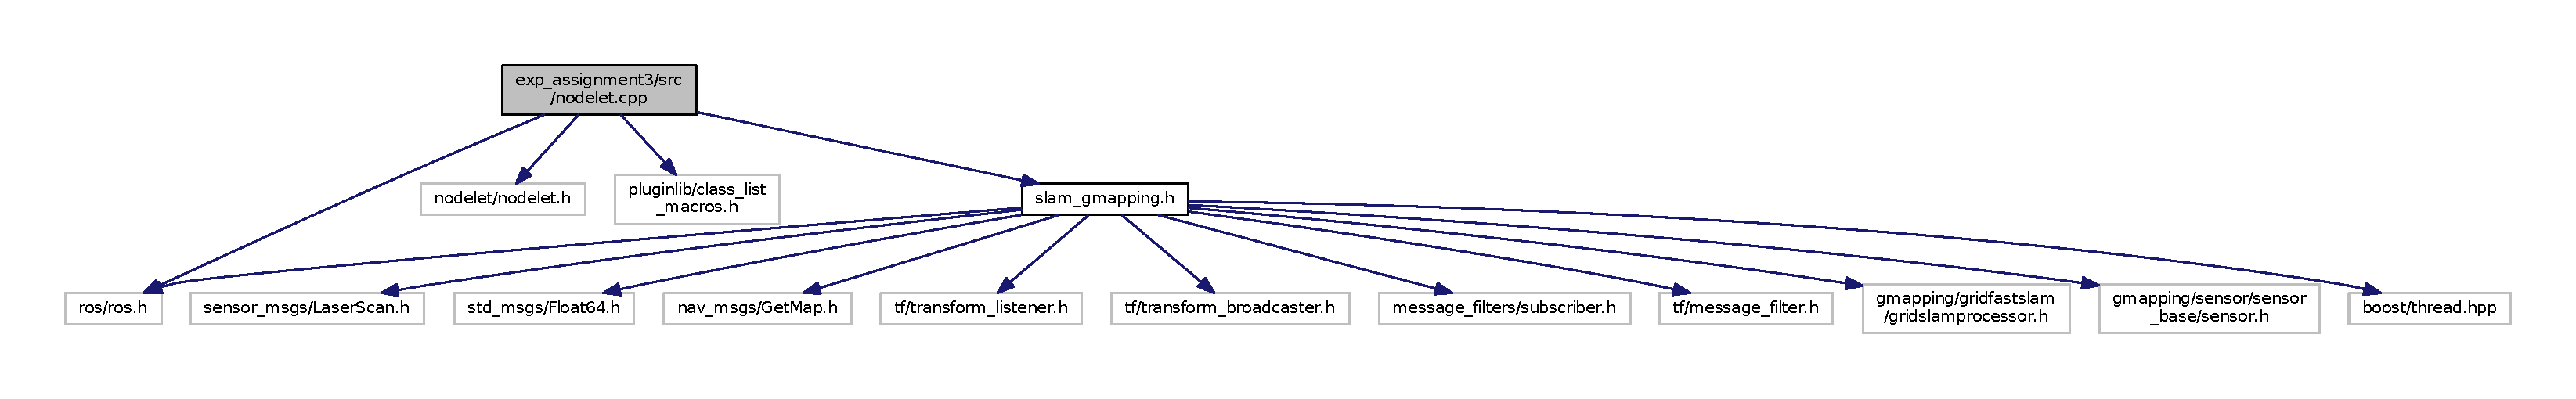
\includegraphics[width=350pt]{nodelet_8cpp__incl}
\end{center}
\end{figure}
\subsection*{Classes}
\begin{DoxyCompactItemize}
\item 
class \hyperlink{classSlamGMappingNodelet}{Slam\+G\+Mapping\+Nodelet}
\end{DoxyCompactItemize}

\hypertarget{replay_8cpp}{}\section{exp\+\_\+assignment3/src/replay.cpp File Reference}
\label{replay_8cpp}\index{exp\+\_\+assignment3/src/replay.\+cpp@{exp\+\_\+assignment3/src/replay.\+cpp}}
{\ttfamily \#include \char`\"{}slam\+\_\+gmapping.\+h\char`\"{}}\\*
{\ttfamily \#include $<$iostream$>$}\\*
{\ttfamily \#include $<$string$>$}\\*
{\ttfamily \#include $<$boost/program\+\_\+options.\+hpp$>$}\\*
{\ttfamily \#include $<$ros/ros.\+h$>$}\\*
Include dependency graph for replay.\+cpp\+:\nopagebreak
\begin{figure}[H]
\begin{center}
\leavevmode
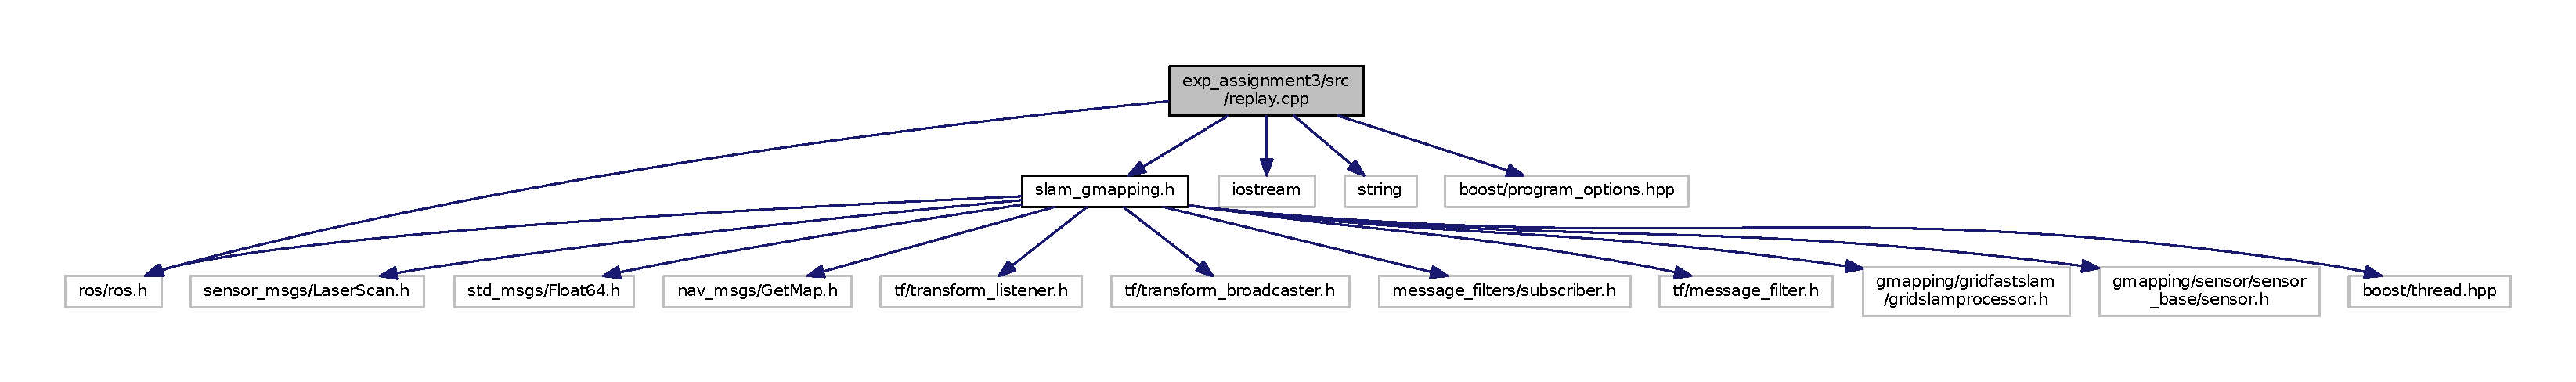
\includegraphics[width=350pt]{replay_8cpp__incl}
\end{center}
\end{figure}
\subsection*{Functions}
\begin{DoxyCompactItemize}
\item 
int \hyperlink{replay_8cpp_a3c04138a5bfe5d72780bb7e82a18e627}{main} (int argc, char $\ast$$\ast$argv)
\end{DoxyCompactItemize}


\subsection{Function Documentation}
\index{replay.\+cpp@{replay.\+cpp}!main@{main}}
\index{main@{main}!replay.\+cpp@{replay.\+cpp}}
\subsubsection[{\texorpdfstring{main(int argc, char $\ast$$\ast$argv)}{main(int argc, char **argv)}}]{\setlength{\rightskip}{0pt plus 5cm}int main (
\begin{DoxyParamCaption}
\item[{int}]{argc, }
\item[{char $\ast$$\ast$}]{argv}
\end{DoxyParamCaption}
)}\hypertarget{replay_8cpp_a3c04138a5bfe5d72780bb7e82a18e627}{}\label{replay_8cpp_a3c04138a5bfe5d72780bb7e82a18e627}
Define and parse the program options

--help option
\hypertarget{slam__gmapping_8h}{}\section{exp\+\_\+assignment3/src/slam\+\_\+gmapping.h File Reference}
\label{slam__gmapping_8h}\index{exp\+\_\+assignment3/src/slam\+\_\+gmapping.\+h@{exp\+\_\+assignment3/src/slam\+\_\+gmapping.\+h}}
{\ttfamily \#include \char`\"{}ros/ros.\+h\char`\"{}}\\*
{\ttfamily \#include \char`\"{}sensor\+\_\+msgs/\+Laser\+Scan.\+h\char`\"{}}\\*
{\ttfamily \#include \char`\"{}std\+\_\+msgs/\+Float64.\+h\char`\"{}}\\*
{\ttfamily \#include \char`\"{}nav\+\_\+msgs/\+Get\+Map.\+h\char`\"{}}\\*
{\ttfamily \#include \char`\"{}tf/transform\+\_\+listener.\+h\char`\"{}}\\*
{\ttfamily \#include \char`\"{}tf/transform\+\_\+broadcaster.\+h\char`\"{}}\\*
{\ttfamily \#include \char`\"{}message\+\_\+filters/subscriber.\+h\char`\"{}}\\*
{\ttfamily \#include \char`\"{}tf/message\+\_\+filter.\+h\char`\"{}}\\*
{\ttfamily \#include \char`\"{}gmapping/gridfastslam/gridslamprocessor.\+h\char`\"{}}\\*
{\ttfamily \#include \char`\"{}gmapping/sensor/sensor\+\_\+base/sensor.\+h\char`\"{}}\\*
{\ttfamily \#include $<$boost/thread.\+hpp$>$}\\*
Include dependency graph for slam\+\_\+gmapping.\+h\+:\nopagebreak
\begin{figure}[H]
\begin{center}
\leavevmode
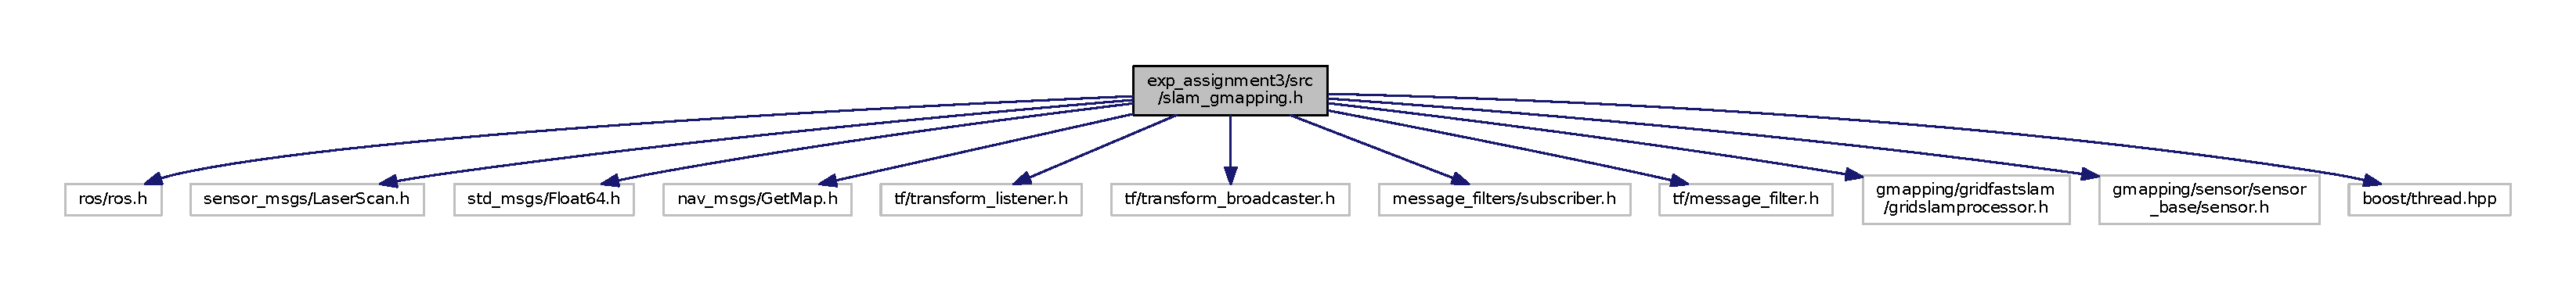
\includegraphics[width=350pt]{slam__gmapping_8h__incl}
\end{center}
\end{figure}
This graph shows which files directly or indirectly include this file\+:\nopagebreak
\begin{figure}[H]
\begin{center}
\leavevmode
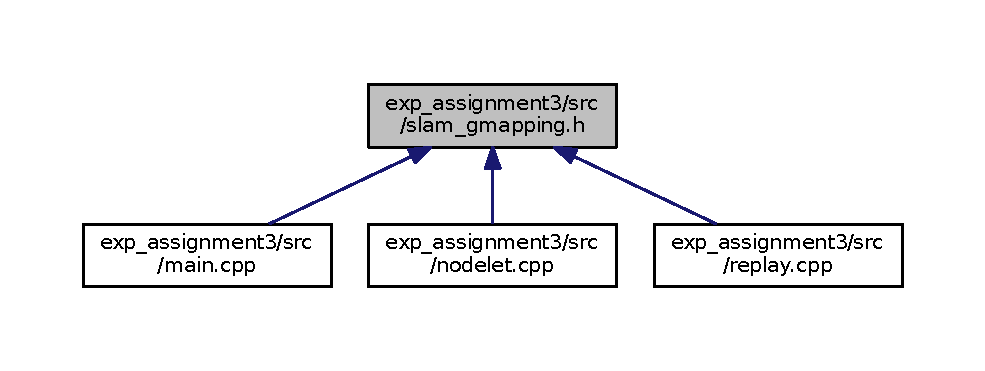
\includegraphics[width=350pt]{slam__gmapping_8h__dep__incl}
\end{center}
\end{figure}
\subsection*{Classes}
\begin{DoxyCompactItemize}
\item 
class \hyperlink{classSlamGMapping}{Slam\+G\+Mapping}
\end{DoxyCompactItemize}

\hypertarget{wiki__doc_8txt}{}\section{m-\/explore/explore/doc/wiki\+\_\+doc.txt File Reference}
\label{wiki__doc_8txt}\index{m-\/explore/explore/doc/wiki\+\_\+doc.\+txt@{m-\/explore/explore/doc/wiki\+\_\+doc.\+txt}}
\subsection*{Functions}
\begin{DoxyCompactItemize}
\item 
$<$$<$ Package\+Header(explore\+\_\+lite)$>$$<$$<$ Git\+Hub\+Issues(hrnr/m-\/explore)$>$$<$$<$ T\+OC(4)$>$ robot will greedily explore its environment until no frontiers could be found Movement commands will be send which makes it easier \hyperlink{wiki__doc_8txt_a59f010b39e38734a32109cf8c8310f81}{to} configure and more \hyperlink{wiki__doc_8txt_af39469afb7931f3c1518b0fc5776008f}{efficient} (lighter on resources).Node simply subscribes \hyperlink{wiki__doc_8txt_a59f010b39e38734a32109cf8c8310f81}{to}$<$$<$ Msg\+Link(nav\+\_\+msgs/Occupancy\+Grid)$>$$>$ messages.\+Commands for robot movement are send \hyperlink{wiki__doc_8txt_a59f010b39e38734a32109cf8c8310f81}{to}\mbox{[}\mbox{[}move\+\_\+base\mbox{]}\mbox{]} node.\+Node can do frontier filtering and can operate even on non-\/inflated maps.\+Goal blacklisting allows \hyperlink{wiki__doc_8txt_a59f010b39e38734a32109cf8c8310f81}{to} deal \hyperlink{wiki__doc_8txt_a110243189100ad190f1295ade52a39a6}{with} places inaccessible for robot.$<$$<$ Youtube(op0\+L0\+Ly\+G\+NwY \&rel=0)$>$$>$
\item 
$<$$<$ Package\+Header(explore\+\_\+lite)$>$$<$$<$ Git\+Hub\+Issues(hrnr/m-\/explore)$>$$<$$<$ T\+OC(4)$>$ robot will greedily explore its environment until no frontiers could be found Movement commands will be send which makes it easier \hyperlink{wiki__doc_8txt_a59f010b39e38734a32109cf8c8310f81}{to} configure and more planning and navigating should work With most planners this should work by refer \hyperlink{wiki__doc_8txt_a59f010b39e38734a32109cf8c8310f81}{to}\mbox{[}\mbox{[}navfn\#Parameters\mbox{]}\mbox{]} if you need \hyperlink{wiki__doc_8txt_a59f010b39e38734a32109cf8c8310f81}{to} setup this for\mbox{[}\mbox{[}navfn\mbox{]}\mbox{]} \hyperlink{wiki__doc_8txt_a1e6f68edc2fdd58ace512f96917cd16e}{planner} (but should be enabled by \hyperlink{wiki__doc_8txt_a2da1dda6a041d7dbeb3aef440c695a60}{default}).Navigation through unknown space is required for
\end{DoxyCompactItemize}
\subsection*{Variables}
\begin{DoxyCompactItemize}
\item 
$<$$<$ Package\+Header(explore\+\_\+lite)$>$$<$$<$ Git\+Hub\+Issues(hrnr/m-\/explore)$>$$<$$<$ T\+OC(4)$>$ robot will greedily explore its environment until no frontiers could be found Movement commands will be send \hyperlink{wiki__doc_8txt_a59f010b39e38734a32109cf8c8310f81}{to} \mbox{[}\mbox{[}move\+\_\+base\mbox{]}\mbox{]}
\item 
$<$$<$ Package\+Header(explore\+\_\+lite)$>$$<$$<$ Git\+Hub\+Issues(hrnr/m-\/explore)$>$$<$$<$ T\+OC(4)$>$ robot will greedily explore its environment until no frontiers could be found Movement commands will be send which makes it easier \hyperlink{wiki__doc_8txt_a59f010b39e38734a32109cf8c8310f81}{to} configure and more planning and navigating should work With most planners this should work by \hyperlink{wiki__doc_8txt_a2da1dda6a041d7dbeb3aef440c695a60}{default}
\item 
If you want \hyperlink{wiki__doc_8txt_a59f010b39e38734a32109cf8c8310f81}{to} use costmap provided by\mbox{[}\mbox{[}move\+\_\+base\mbox{]}\mbox{]} you need \hyperlink{wiki__doc_8txt_a59f010b39e38734a32109cf8c8310f81}{to} enable unknown space tracking by setting \hyperlink{wiki__doc_8txt_aae8355eda2c5eda5fc33ae2b62ba937c}{track\+\_\+unknown\+\_\+space}
\item 
If you want \hyperlink{wiki__doc_8txt_a59f010b39e38734a32109cf8c8310f81}{to} use costmap provided by\mbox{[}\mbox{[}move\+\_\+base\mbox{]}\mbox{]} you need \hyperlink{wiki__doc_8txt_a59f010b39e38734a32109cf8c8310f81}{to} enable unknown space tracking by setting you can start experimenting \hyperlink{wiki__doc_8txt_a110243189100ad190f1295ade52a39a6}{with} \{\{\{explore\+\_\+lite\}\}\}. Provided `explore.\+launch` should work out-\/of-\/the box in most cases
\end{DoxyCompactItemize}


\subsection{Function Documentation}
\index{wiki\+\_\+doc.\+txt@{wiki\+\_\+doc.\+txt}!efficient@{efficient}}
\index{efficient@{efficient}!wiki\+\_\+doc.\+txt@{wiki\+\_\+doc.\+txt}}
\subsubsection[{\texorpdfstring{efficient(lighter on resources).\+Node simply subscribes to$<$$<$ Msg\+Link(nav\+\_\+msgs/\+Occupancy\+Grid)$>$$>$ messages.\+Commands for robot movement are send to[[move\+\_\+base]] node.\+Node can do frontier filtering and can operate even on non-\/inflated maps.\+Goal blacklisting allows to deal with places inaccessible for robot.$<$$<$ Youtube(op0\+L0\+Ly\+G\+Nw\+Y \&rel=0)$>$$>$}{efficient(lighter on resources).Node simply subscribes to<< MsgLink(nav_msgs/OccupancyGrid)>> messages.Commands for robot movement are send to[[move_base]] node.Node can do frontier filtering and can operate even on non-inflated maps.Goal blacklisting allows to deal with places inaccessible for robot.<< Youtube(op0L0LyGNwY &rel=0)>>}}]{\setlength{\rightskip}{0pt plus 5cm}$<$$<$Package\+Header(explore\+\_\+lite)$>$$<$$<$Git\+Hub\+Issues(hrnr/m-\/explore)$>$$<$$<$T\+OC(4)$>$ robot will greedily explore its environment until no frontiers could be found Movement commands will be send which makes it easier {\bf to} configure and more efficient (
\begin{DoxyParamCaption}
\item[{lighter on}]{resources}
\end{DoxyParamCaption}
)\hspace{0.3cm}{\ttfamily [pure virtual]}}\hypertarget{wiki__doc_8txt_af39469afb7931f3c1518b0fc5776008f}{}\label{wiki__doc_8txt_af39469afb7931f3c1518b0fc5776008f}
\index{wiki\+\_\+doc.\+txt@{wiki\+\_\+doc.\+txt}!planner@{planner}}
\index{planner@{planner}!wiki\+\_\+doc.\+txt@{wiki\+\_\+doc.\+txt}}
\subsubsection[{\texorpdfstring{planner(but should be enabled by default).\+Navigation through unknown space is required for}{planner(but should be enabled by default).Navigation through unknown space is required for}}]{\setlength{\rightskip}{0pt plus 5cm}$<$$<$Package\+Header(explore\+\_\+lite)$>$$<$$<$Git\+Hub\+Issues(hrnr/m-\/explore)$>$$<$$<$T\+OC(4)$>$ robot will greedily explore its environment until no frontiers could be found Movement commands will be send which makes it easier {\bf to} configure and more planning and navigating should work With most planners this should work by refer {\bf to} \mbox{[}\mbox{[}navfn\#Parameters\mbox{]}\mbox{]} if you need {\bf to} setup this for \mbox{[}\mbox{[}navfn\mbox{]}\mbox{]} planner (
\begin{DoxyParamCaption}
\item[{but should be enabled by}]{default}
\end{DoxyParamCaption}
)}\hypertarget{wiki__doc_8txt_a1e6f68edc2fdd58ace512f96917cd16e}{}\label{wiki__doc_8txt_a1e6f68edc2fdd58ace512f96917cd16e}


\subsection{Variable Documentation}
\index{wiki\+\_\+doc.\+txt@{wiki\+\_\+doc.\+txt}!default@{default}}
\index{default@{default}!wiki\+\_\+doc.\+txt@{wiki\+\_\+doc.\+txt}}
\subsubsection[{\texorpdfstring{default}{default}}]{\setlength{\rightskip}{0pt plus 5cm}$<$$<$Package\+Header(explore\+\_\+lite)$>$$<$$<$Git\+Hub\+Issues(hrnr/m-\/explore)$>$$<$$<$T\+OC(4)$>$ robot will greedily explore its environment until no frontiers could be found Movement commands will be send which makes it easier {\bf to} configure and more planning and navigating should work With most planners this should work by default}\hypertarget{wiki__doc_8txt_a2da1dda6a041d7dbeb3aef440c695a60}{}\label{wiki__doc_8txt_a2da1dda6a041d7dbeb3aef440c695a60}
\index{wiki\+\_\+doc.\+txt@{wiki\+\_\+doc.\+txt}!to@{to}}
\index{to@{to}!wiki\+\_\+doc.\+txt@{wiki\+\_\+doc.\+txt}}
\subsubsection[{\texorpdfstring{to}{to}}]{\setlength{\rightskip}{0pt plus 5cm}$<$$<$Package\+Header(explore\+\_\+lite)$>$$<$$<$Git\+Hub\+Issues(hrnr/m-\/explore)$>$$<$$<$T\+OC(4)$>$ robot will greedily explore its environment until no frontiers could be found Movement commands will be send to\mbox{[}\mbox{[}move\+\_\+base\mbox{]}\mbox{]}}\hypertarget{wiki__doc_8txt_a59f010b39e38734a32109cf8c8310f81}{}\label{wiki__doc_8txt_a59f010b39e38734a32109cf8c8310f81}
{\bfseries Initial value\+:}
\begin{DoxyCode}
\{\{attachment:screenshot.png||width=\textcolor{stringliteral}{"755px"}\}\}

Unlike similar packages
\end{DoxyCode}
\index{wiki\+\_\+doc.\+txt@{wiki\+\_\+doc.\+txt}!track\+\_\+unknown\+\_\+space@{track\+\_\+unknown\+\_\+space}}
\index{track\+\_\+unknown\+\_\+space@{track\+\_\+unknown\+\_\+space}!wiki\+\_\+doc.\+txt@{wiki\+\_\+doc.\+txt}}
\subsubsection[{\texorpdfstring{track\+\_\+unknown\+\_\+space}{track_unknown_space}}]{\setlength{\rightskip}{0pt plus 5cm}If you want {\bf to} use costmap provided by \mbox{[}\mbox{[}move\+\_\+base\mbox{]}\mbox{]} you need {\bf to} enable unknown space tracking by setting track\+\_\+unknown\+\_\+space}\hypertarget{wiki__doc_8txt_aae8355eda2c5eda5fc33ae2b62ba937c}{}\label{wiki__doc_8txt_aae8355eda2c5eda5fc33ae2b62ba937c}
\index{wiki\+\_\+doc.\+txt@{wiki\+\_\+doc.\+txt}!with@{with}}
\index{with@{with}!wiki\+\_\+doc.\+txt@{wiki\+\_\+doc.\+txt}}
\subsubsection[{\texorpdfstring{with}{with}}]{\setlength{\rightskip}{0pt plus 5cm}If you want {\bf to} use costmap provided by \mbox{[}\mbox{[}move\+\_\+base\mbox{]}\mbox{]} you need {\bf to} enable unknown space tracking by setting you can start experimenting with \{\{\{explore\+\_\+lite\}\}\}. Provided `explore.\+launch` should work out-\/of-\/the box in most cases}\hypertarget{wiki__doc_8txt_a110243189100ad190f1295ade52a39a6}{}\label{wiki__doc_8txt_a110243189100ad190f1295ade52a39a6}

\hypertarget{costmap__client_8h}{}\section{m-\/explore/explore/include/explore/costmap\+\_\+client.h File Reference}
\label{costmap__client_8h}\index{m-\/explore/explore/include/explore/costmap\+\_\+client.\+h@{m-\/explore/explore/include/explore/costmap\+\_\+client.\+h}}
{\ttfamily \#include $<$costmap\+\_\+2d/costmap\+\_\+2d.\+h$>$}\\*
{\ttfamily \#include $<$geometry\+\_\+msgs/\+Pose.\+h$>$}\\*
{\ttfamily \#include $<$map\+\_\+msgs/\+Occupancy\+Grid\+Update.\+h$>$}\\*
{\ttfamily \#include $<$nav\+\_\+msgs/\+Occupancy\+Grid.\+h$>$}\\*
{\ttfamily \#include $<$ros/ros.\+h$>$}\\*
{\ttfamily \#include $<$tf/tf.\+h$>$}\\*
{\ttfamily \#include $<$tf/transform\+\_\+listener.\+h$>$}\\*
Include dependency graph for costmap\+\_\+client.\+h\+:\nopagebreak
\begin{figure}[H]
\begin{center}
\leavevmode
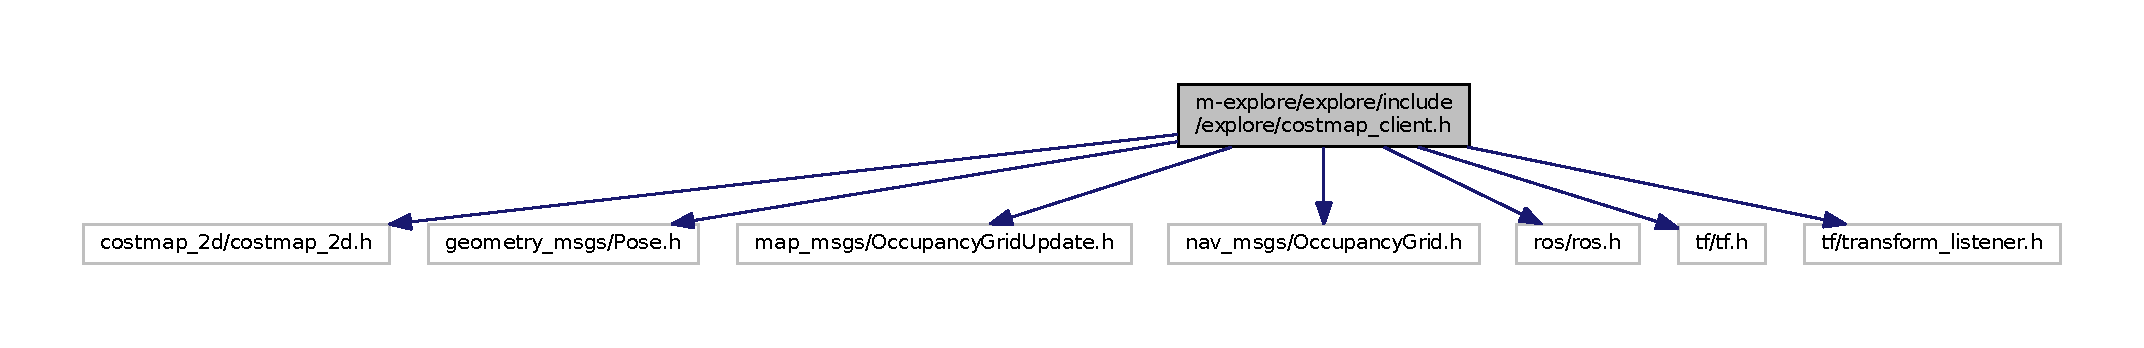
\includegraphics[width=350pt]{costmap__client_8h__incl}
\end{center}
\end{figure}
This graph shows which files directly or indirectly include this file\+:\nopagebreak
\begin{figure}[H]
\begin{center}
\leavevmode
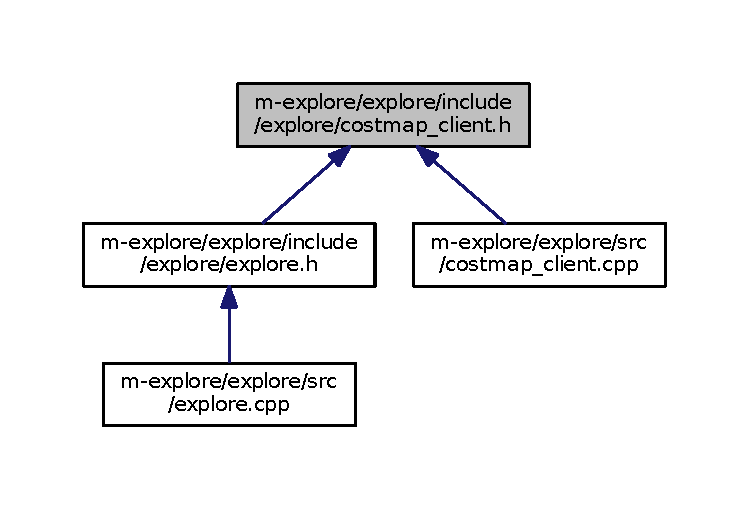
\includegraphics[width=350pt]{costmap__client_8h__dep__incl}
\end{center}
\end{figure}
\subsection*{Classes}
\begin{DoxyCompactItemize}
\item 
class \hyperlink{classexplore_1_1Costmap2DClient}{explore\+::\+Costmap2\+D\+Client}
\end{DoxyCompactItemize}
\subsection*{Namespaces}
\begin{DoxyCompactItemize}
\item 
 \hyperlink{namespaceexplore}{explore}
\end{DoxyCompactItemize}

\hypertarget{costmap__tools_8h}{}\section{m-\/explore/explore/include/explore/costmap\+\_\+tools.h File Reference}
\label{costmap__tools_8h}\index{m-\/explore/explore/include/explore/costmap\+\_\+tools.\+h@{m-\/explore/explore/include/explore/costmap\+\_\+tools.\+h}}
{\ttfamily \#include $<$costmap\+\_\+2d/costmap\+\_\+2d.\+h$>$}\\*
{\ttfamily \#include $<$geometry\+\_\+msgs/\+Point\+Stamped.\+h$>$}\\*
{\ttfamily \#include $<$geometry\+\_\+msgs/\+Polygon\+Stamped.\+h$>$}\\*
{\ttfamily \#include $<$ros/ros.\+h$>$}\\*
Include dependency graph for costmap\+\_\+tools.\+h\+:\nopagebreak
\begin{figure}[H]
\begin{center}
\leavevmode
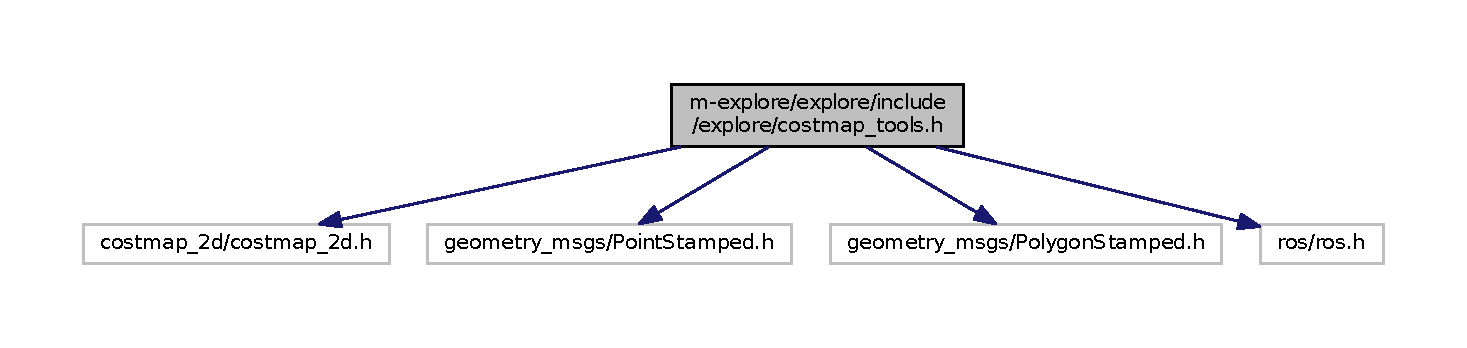
\includegraphics[width=350pt]{costmap__tools_8h__incl}
\end{center}
\end{figure}
This graph shows which files directly or indirectly include this file\+:\nopagebreak
\begin{figure}[H]
\begin{center}
\leavevmode
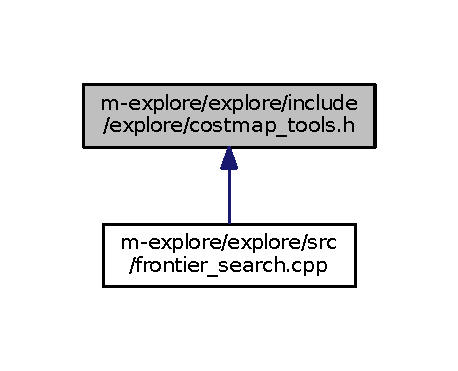
\includegraphics[width=220pt]{costmap__tools_8h__dep__incl}
\end{center}
\end{figure}
\subsection*{Namespaces}
\begin{DoxyCompactItemize}
\item 
 \hyperlink{namespacefrontier__exploration}{frontier\+\_\+exploration}
\end{DoxyCompactItemize}
\subsection*{Functions}
\begin{DoxyCompactItemize}
\item 
std\+::vector$<$ unsigned int $>$ \hyperlink{namespacefrontier__exploration_affc5c02b52db13456c62dc5f707efa6f}{frontier\+\_\+exploration\+::nhood4} (unsigned int idx, const costmap\+\_\+2d\+::\+Costmap2D \&costmap)
\begin{DoxyCompactList}\small\item\em Determine 4-\/connected neighbourhood of an input cell, checking for map edges. \end{DoxyCompactList}\item 
std\+::vector$<$ unsigned int $>$ \hyperlink{namespacefrontier__exploration_aff5530dc70914d4cfde4f455ecaa0cd6}{frontier\+\_\+exploration\+::nhood8} (unsigned int idx, const costmap\+\_\+2d\+::\+Costmap2D \&costmap)
\begin{DoxyCompactList}\small\item\em Determine 8-\/connected neighbourhood of an input cell, checking for map edges. \end{DoxyCompactList}\item 
bool \hyperlink{namespacefrontier__exploration_a1919c053e430083b7fb366501fff518c}{frontier\+\_\+exploration\+::nearest\+Cell} (unsigned int \&result, unsigned int start, unsigned char val, const costmap\+\_\+2d\+::\+Costmap2D \&costmap)
\begin{DoxyCompactList}\small\item\em Find nearest cell of a specified value. \end{DoxyCompactList}\end{DoxyCompactItemize}

\hypertarget{explore_8h}{}\section{m-\/explore/explore/include/explore/explore.h File Reference}
\label{explore_8h}\index{m-\/explore/explore/include/explore/explore.\+h@{m-\/explore/explore/include/explore/explore.\+h}}
{\ttfamily \#include $<$memory$>$}\\*
{\ttfamily \#include $<$mutex$>$}\\*
{\ttfamily \#include $<$string$>$}\\*
{\ttfamily \#include $<$vector$>$}\\*
{\ttfamily \#include $<$actionlib/client/simple\+\_\+action\+\_\+client.\+h$>$}\\*
{\ttfamily \#include $<$geometry\+\_\+msgs/\+Pose\+Stamped.\+h$>$}\\*
{\ttfamily \#include $<$move\+\_\+base\+\_\+msgs/\+Move\+Base\+Action.\+h$>$}\\*
{\ttfamily \#include $<$ros/ros.\+h$>$}\\*
{\ttfamily \#include $<$visualization\+\_\+msgs/\+Marker\+Array.\+h$>$}\\*
{\ttfamily \#include $<$explore/costmap\+\_\+client.\+h$>$}\\*
{\ttfamily \#include $<$explore/frontier\+\_\+search.\+h$>$}\\*
Include dependency graph for explore.\+h\+:\nopagebreak
\begin{figure}[H]
\begin{center}
\leavevmode
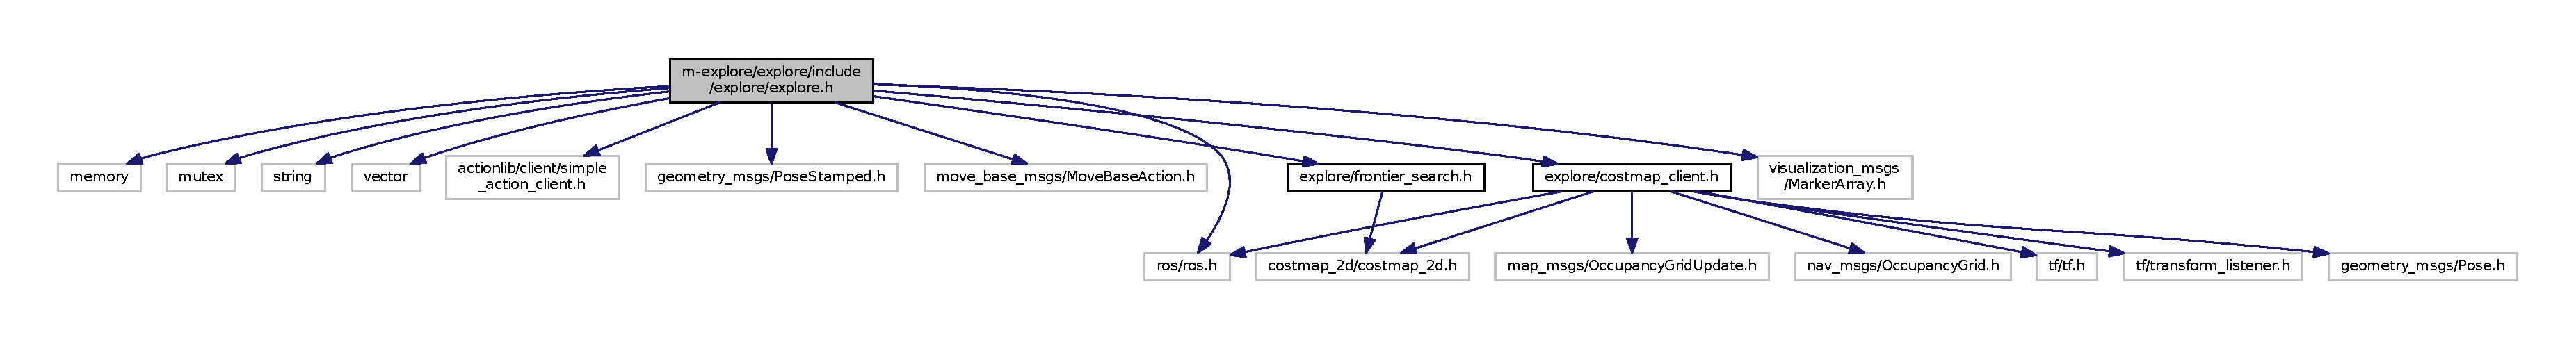
\includegraphics[width=350pt]{explore_8h__incl}
\end{center}
\end{figure}
This graph shows which files directly or indirectly include this file\+:\nopagebreak
\begin{figure}[H]
\begin{center}
\leavevmode
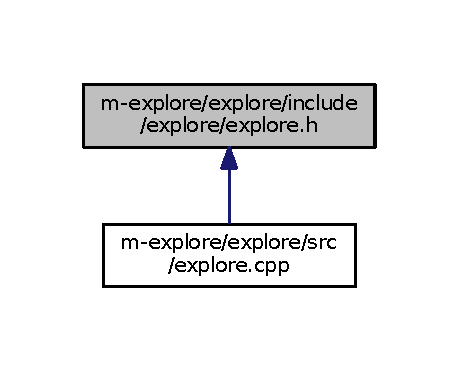
\includegraphics[width=220pt]{explore_8h__dep__incl}
\end{center}
\end{figure}
\subsection*{Classes}
\begin{DoxyCompactItemize}
\item 
class \hyperlink{classexplore_1_1Explore}{explore\+::\+Explore}
\begin{DoxyCompactList}\small\item\em A class adhering to the robot\+\_\+actions\+::\+Action interface that moves the robot base to explore its environment. \end{DoxyCompactList}\end{DoxyCompactItemize}
\subsection*{Namespaces}
\begin{DoxyCompactItemize}
\item 
 \hyperlink{namespaceexplore}{explore}
\end{DoxyCompactItemize}

\hypertarget{frontier__search_8h}{}\section{m-\/explore/explore/include/explore/frontier\+\_\+search.h File Reference}
\label{frontier__search_8h}\index{m-\/explore/explore/include/explore/frontier\+\_\+search.\+h@{m-\/explore/explore/include/explore/frontier\+\_\+search.\+h}}
{\ttfamily \#include $<$costmap\+\_\+2d/costmap\+\_\+2d.\+h$>$}\\*
Include dependency graph for frontier\+\_\+search.\+h\+:\nopagebreak
\begin{figure}[H]
\begin{center}
\leavevmode
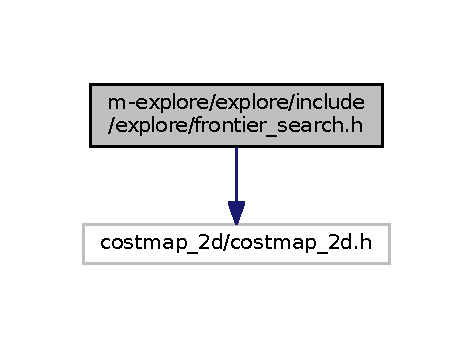
\includegraphics[width=227pt]{frontier__search_8h__incl}
\end{center}
\end{figure}
This graph shows which files directly or indirectly include this file\+:\nopagebreak
\begin{figure}[H]
\begin{center}
\leavevmode
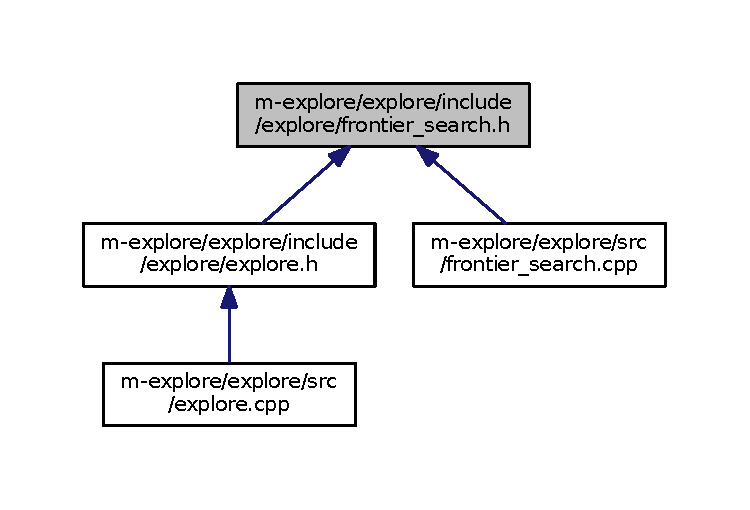
\includegraphics[width=350pt]{frontier__search_8h__dep__incl}
\end{center}
\end{figure}
\subsection*{Classes}
\begin{DoxyCompactItemize}
\item 
struct \hyperlink{structfrontier__exploration_1_1Frontier}{frontier\+\_\+exploration\+::\+Frontier}
\begin{DoxyCompactList}\small\item\em Represents a frontier. \end{DoxyCompactList}\item 
class \hyperlink{classfrontier__exploration_1_1FrontierSearch}{frontier\+\_\+exploration\+::\+Frontier\+Search}
\begin{DoxyCompactList}\small\item\em Thread-\/safe implementation of a frontier-\/search task for an input costmap. \end{DoxyCompactList}\end{DoxyCompactItemize}
\subsection*{Namespaces}
\begin{DoxyCompactItemize}
\item 
 \hyperlink{namespacefrontier__exploration}{frontier\+\_\+exploration}
\end{DoxyCompactItemize}

\hypertarget{costmap__client_8cpp}{}\section{m-\/explore/explore/src/costmap\+\_\+client.cpp File Reference}
\label{costmap__client_8cpp}\index{m-\/explore/explore/src/costmap\+\_\+client.\+cpp@{m-\/explore/explore/src/costmap\+\_\+client.\+cpp}}
{\ttfamily \#include $<$explore/costmap\+\_\+client.\+h$>$}\\*
{\ttfamily \#include $<$functional$>$}\\*
{\ttfamily \#include $<$mutex$>$}\\*
{\ttfamily \#include $<$string$>$}\\*
Include dependency graph for costmap\+\_\+client.\+cpp\+:\nopagebreak
\begin{figure}[H]
\begin{center}
\leavevmode
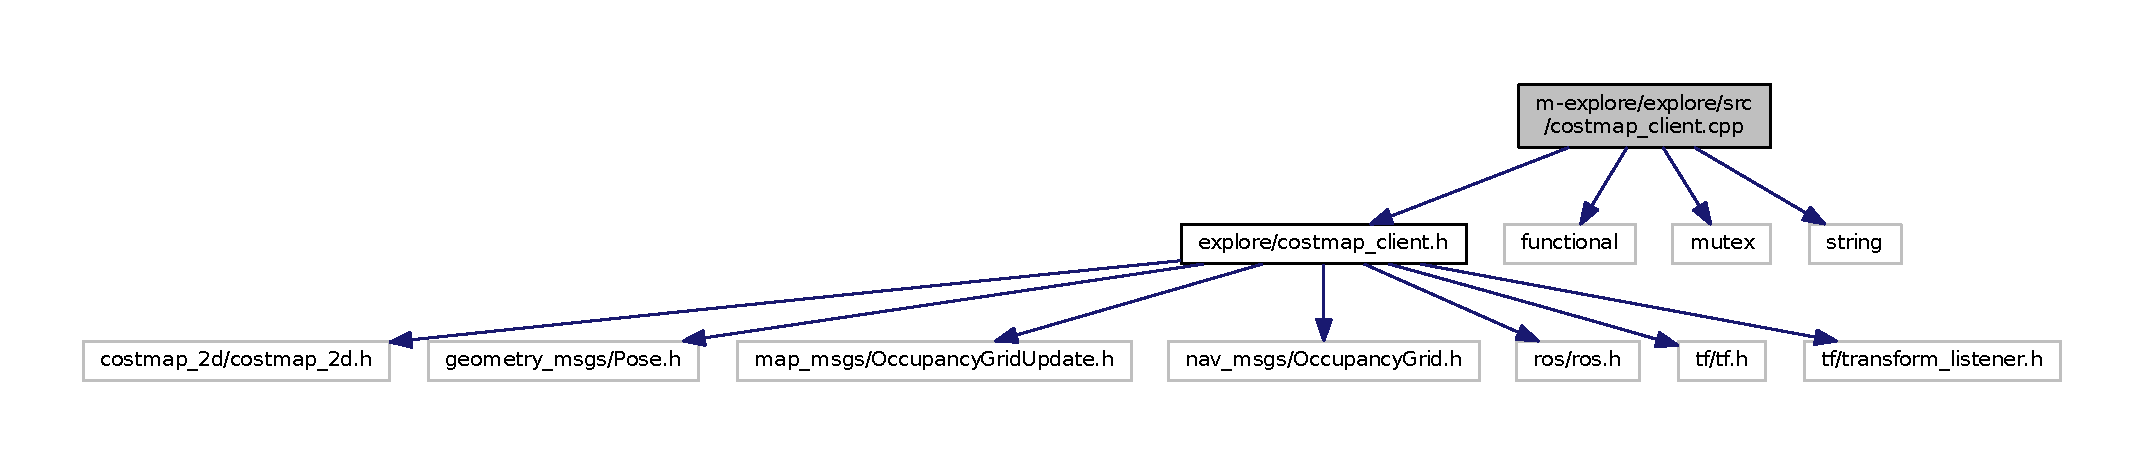
\includegraphics[width=350pt]{costmap__client_8cpp__incl}
\end{center}
\end{figure}
\subsection*{Namespaces}
\begin{DoxyCompactItemize}
\item 
 \hyperlink{namespaceexplore}{explore}
\end{DoxyCompactItemize}
\subsection*{Functions}
\begin{DoxyCompactItemize}
\item 
std\+::array$<$ unsigned char, 256 $>$ \hyperlink{namespaceexplore_a10c3d97c3a8b11559b94afafa1348c38}{explore\+::init\+\_\+translation\+\_\+table} ()
\end{DoxyCompactItemize}

\hypertarget{explore_8cpp}{}\section{m-\/explore/explore/src/explore.cpp File Reference}
\label{explore_8cpp}\index{m-\/explore/explore/src/explore.\+cpp@{m-\/explore/explore/src/explore.\+cpp}}
{\ttfamily \#include $<$explore/explore.\+h$>$}\\*
{\ttfamily \#include $<$thread$>$}\\*
Include dependency graph for explore.\+cpp\+:\nopagebreak
\begin{figure}[H]
\begin{center}
\leavevmode
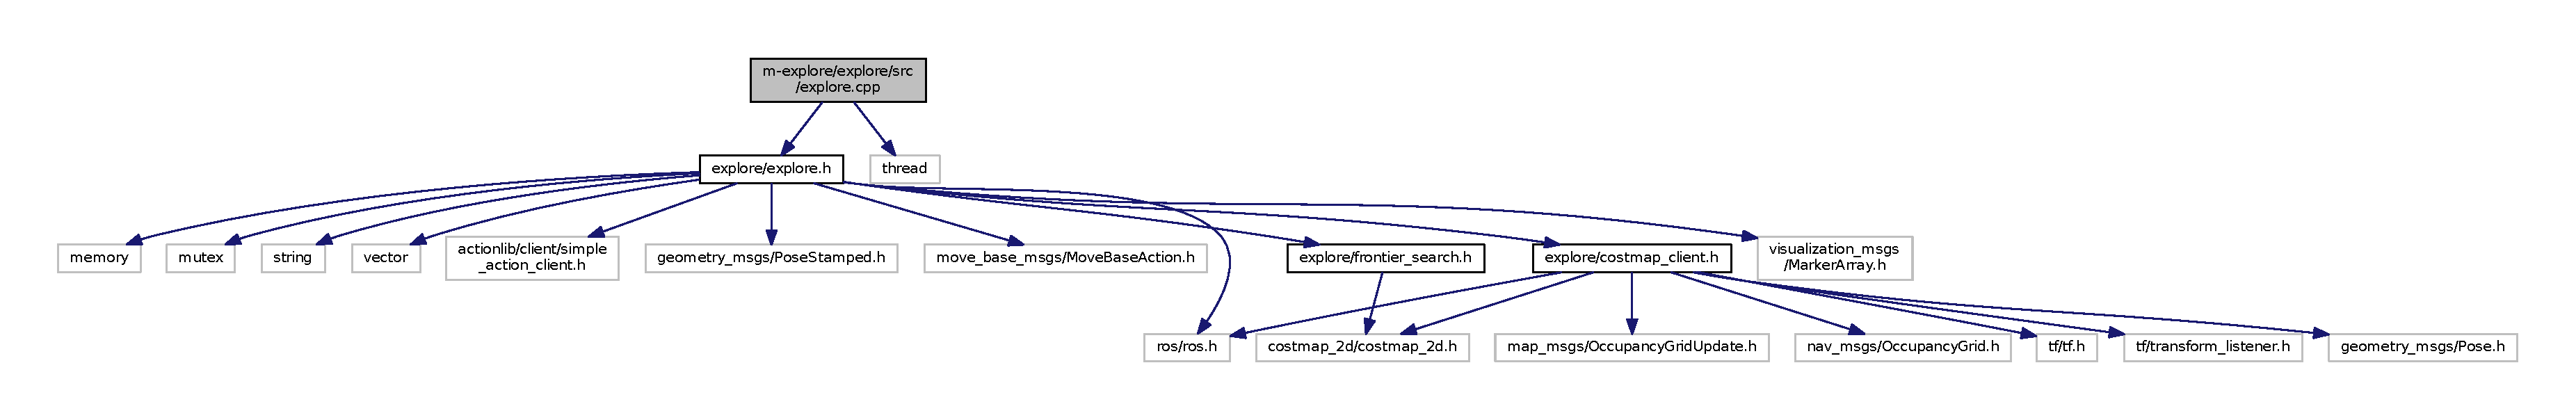
\includegraphics[width=350pt]{explore_8cpp__incl}
\end{center}
\end{figure}
\subsection*{Namespaces}
\begin{DoxyCompactItemize}
\item 
 \hyperlink{namespaceexplore}{explore}
\end{DoxyCompactItemize}
\subsection*{Functions}
\begin{DoxyCompactItemize}
\item 
int \hyperlink{explore_8cpp_a3c04138a5bfe5d72780bb7e82a18e627}{main} (int argc, char $\ast$$\ast$argv)
\end{DoxyCompactItemize}


\subsection{Function Documentation}
\index{explore.\+cpp@{explore.\+cpp}!main@{main}}
\index{main@{main}!explore.\+cpp@{explore.\+cpp}}
\subsubsection[{\texorpdfstring{main(int argc, char $\ast$$\ast$argv)}{main(int argc, char **argv)}}]{\setlength{\rightskip}{0pt plus 5cm}int main (
\begin{DoxyParamCaption}
\item[{int}]{argc, }
\item[{char $\ast$$\ast$}]{argv}
\end{DoxyParamCaption}
)}\hypertarget{explore_8cpp_a3c04138a5bfe5d72780bb7e82a18e627}{}\label{explore_8cpp_a3c04138a5bfe5d72780bb7e82a18e627}

\hypertarget{frontier__search_8cpp}{}\section{m-\/explore/explore/src/frontier\+\_\+search.cpp File Reference}
\label{frontier__search_8cpp}\index{m-\/explore/explore/src/frontier\+\_\+search.\+cpp@{m-\/explore/explore/src/frontier\+\_\+search.\+cpp}}
{\ttfamily \#include $<$explore/frontier\+\_\+search.\+h$>$}\\*
{\ttfamily \#include $<$mutex$>$}\\*
{\ttfamily \#include $<$costmap\+\_\+2d/cost\+\_\+values.\+h$>$}\\*
{\ttfamily \#include $<$costmap\+\_\+2d/costmap\+\_\+2d.\+h$>$}\\*
{\ttfamily \#include $<$geometry\+\_\+msgs/\+Point.\+h$>$}\\*
{\ttfamily \#include $<$explore/costmap\+\_\+tools.\+h$>$}\\*
Include dependency graph for frontier\+\_\+search.\+cpp\+:\nopagebreak
\begin{figure}[H]
\begin{center}
\leavevmode
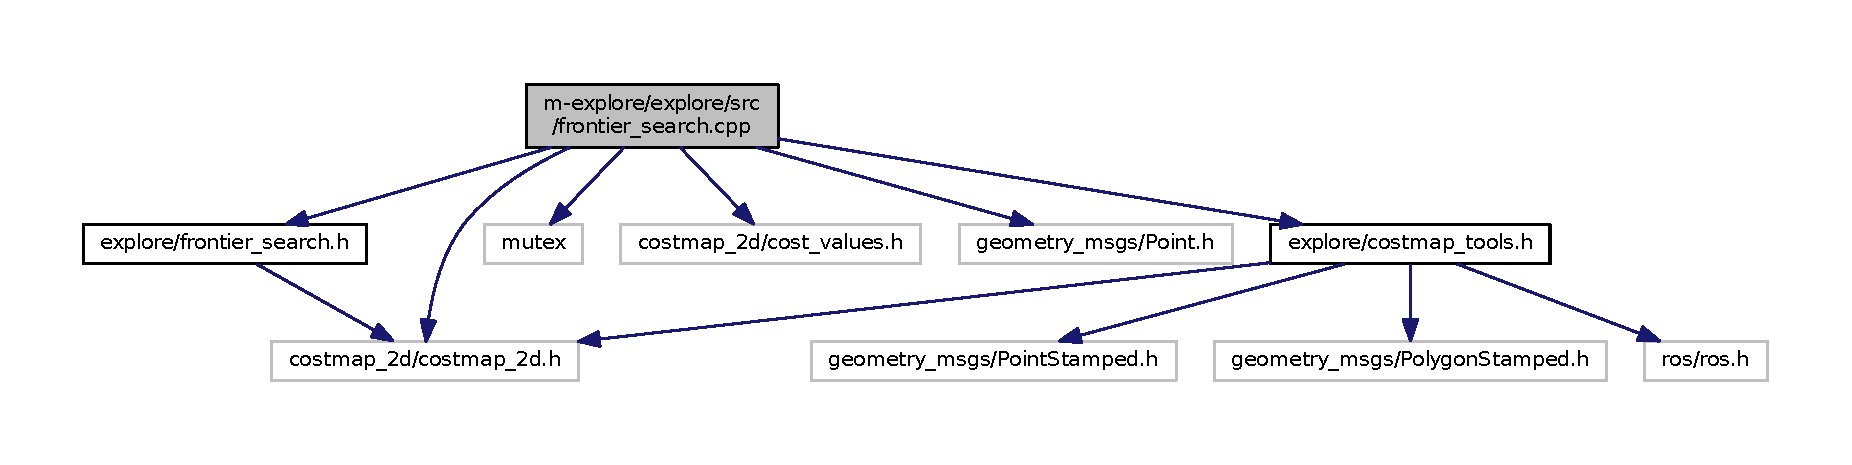
\includegraphics[width=350pt]{frontier__search_8cpp__incl}
\end{center}
\end{figure}
\subsection*{Namespaces}
\begin{DoxyCompactItemize}
\item 
 \hyperlink{namespacefrontier__exploration}{frontier\+\_\+exploration}
\end{DoxyCompactItemize}

\hypertarget{readme__explore_8md}{}\section{m-\/explore/readme\+\_\+explore.md File Reference}
\label{readme__explore_8md}\index{m-\/explore/readme\+\_\+explore.\+md@{m-\/explore/readme\+\_\+explore.\+md}}

\hypertarget{placeholder_8txt}{}\section{Media/placeholder.txt File Reference}
\label{placeholder_8txt}\index{Media/placeholder.\+txt@{Media/placeholder.\+txt}}

\hypertarget{go__to__point_8py}{}\section{motion\+\_\+plan/scripts/go\+\_\+to\+\_\+point.py File Reference}
\label{go__to__point_8py}\index{motion\+\_\+plan/scripts/go\+\_\+to\+\_\+point.\+py@{motion\+\_\+plan/scripts/go\+\_\+to\+\_\+point.\+py}}
\subsection*{Namespaces}
\begin{DoxyCompactItemize}
\item 
 \hyperlink{namespacego__to__point}{go\+\_\+to\+\_\+point}
\end{DoxyCompactItemize}
\subsection*{Functions}
\begin{DoxyCompactItemize}
\item 
def \hyperlink{namespacego__to__point_a36304a9f313b0579f7fc69fa01695524}{go\+\_\+to\+\_\+point.\+clbk\+\_\+odom} (msg)
\item 
def \hyperlink{namespacego__to__point_a31ee48e5cae36821049b572a96b7c8be}{go\+\_\+to\+\_\+point.\+change\+\_\+state} (state)
\item 
def \hyperlink{namespacego__to__point_ac688bb56fa84763ea2edefc30cae032a}{go\+\_\+to\+\_\+point.\+normalize\+\_\+angle} (angle)
\item 
def \hyperlink{namespacego__to__point_a9c3011a3065fcbefcc1c5ad8c9979669}{go\+\_\+to\+\_\+point.\+fix\+\_\+yaw} (des\+\_\+pos)
\item 
def \hyperlink{namespacego__to__point_ac8579665c0fbf665f734476554fac37d}{go\+\_\+to\+\_\+point.\+go\+\_\+straight\+\_\+ahead} (des\+\_\+pos)
\item 
def \hyperlink{namespacego__to__point_ac2587220a4ac9c845bc9c5b0b45d5835}{go\+\_\+to\+\_\+point.\+done} ()
\item 
def \hyperlink{namespacego__to__point_ab92bd6db1ec323a4d795ed6cb40aebe1}{go\+\_\+to\+\_\+point.\+main} ()
\end{DoxyCompactItemize}
\subsection*{Variables}
\begin{DoxyCompactItemize}
\item 
\hyperlink{namespacego__to__point_a500520cbcd448f46bf7447a431f61d53}{go\+\_\+to\+\_\+point.\+position\+\_\+} = Point()
\item 
int \hyperlink{namespacego__to__point_ae444f19eb2019982432760ace036ce03}{go\+\_\+to\+\_\+point.\+yaw\+\_\+} = 0
\item 
int \hyperlink{namespacego__to__point_aa2d0ef255bcf5d5faf9ca2764730fb17}{go\+\_\+to\+\_\+point.\+state\+\_\+} = 0
\item 
\hyperlink{namespacego__to__point_a03b48b610dbd224a38eb226c1b2ba23d}{go\+\_\+to\+\_\+point.\+desired\+\_\+position\+\_\+} = Point()
\item 
\hyperlink{namespacego__to__point_a328c9a3bb9322f150f2e67371cd73306}{go\+\_\+to\+\_\+point.\+x}
\item 
\hyperlink{namespacego__to__point_ac372e1a492f9aa66d29f365cc1c57d8c}{go\+\_\+to\+\_\+point.\+y}
\item 
\hyperlink{namespacego__to__point_a2fd68a76b8583598a4bceccdeae5d73b}{go\+\_\+to\+\_\+point.\+z}
\item 
int \hyperlink{namespacego__to__point_a67f95834f0959feb3facd17bc7fa2b38}{go\+\_\+to\+\_\+point.\+yaw\+\_\+precision\+\_\+} = math.\+pi/9
\item 
int \hyperlink{namespacego__to__point_af74ccf49164d0478ca8343e2031d5813}{go\+\_\+to\+\_\+point.\+yaw\+\_\+precision\+\_\+2\+\_\+} = math.\+pi/90
\item 
float \hyperlink{namespacego__to__point_a6a1e4eb20ebd4fce0fc56b0ebfd7a8d5}{go\+\_\+to\+\_\+point.\+dist\+\_\+precision\+\_\+} = 0.\+1
\item 
float \hyperlink{namespacego__to__point_a524106fc7667a0927951dfd89d52d6a7}{go\+\_\+to\+\_\+point.\+kp\+\_\+a} = 3.\+0
\item 
float \hyperlink{namespacego__to__point_a7bc498652ca66932e704e738b50c297b}{go\+\_\+to\+\_\+point.\+kp\+\_\+d} = 0.\+2
\item 
float \hyperlink{namespacego__to__point_acb4e14986fafe5cb73bb8ad0c178869d}{go\+\_\+to\+\_\+point.\+ub\+\_\+a} = 0.\+6
\item 
float \hyperlink{namespacego__to__point_afecad4058844db05d8321199e25b4498}{go\+\_\+to\+\_\+point.\+lb\+\_\+a} = -\/0.\+5
\item 
float \hyperlink{namespacego__to__point_a16c473b9e717200c483d18e66b48152a}{go\+\_\+to\+\_\+point.\+ub\+\_\+d} = 0.\+6
\item 
\hyperlink{namespacego__to__point_a3caa5a6c1e8d7b4854f62a9e35dfad6f}{go\+\_\+to\+\_\+point.\+pub} = None
\end{DoxyCompactItemize}

\hypertarget{move__client_8cpp}{}\section{motion\+\_\+plan/src/move\+\_\+client.cpp File Reference}
\label{move__client_8cpp}\index{motion\+\_\+plan/src/move\+\_\+client.\+cpp@{motion\+\_\+plan/src/move\+\_\+client.\+cpp}}
{\ttfamily \#include $<$ros/ros.\+h$>$}\\*
{\ttfamily \#include $<$motion\+\_\+plan/\+Planning\+Action.\+h$>$}\\*
{\ttfamily \#include $<$actionlib/client/simple\+\_\+action\+\_\+client.\+h$>$}\\*
{\ttfamily \#include $<$actionlib/client/terminal\+\_\+state.\+h$>$}\\*
{\ttfamily \#include $<$std\+\_\+msgs/\+Float64.\+h$>$}\\*
{\ttfamily \#include $<$unistd.\+h$>$}\\*
Include dependency graph for move\+\_\+client.\+cpp\+:\nopagebreak
\begin{figure}[H]
\begin{center}
\leavevmode
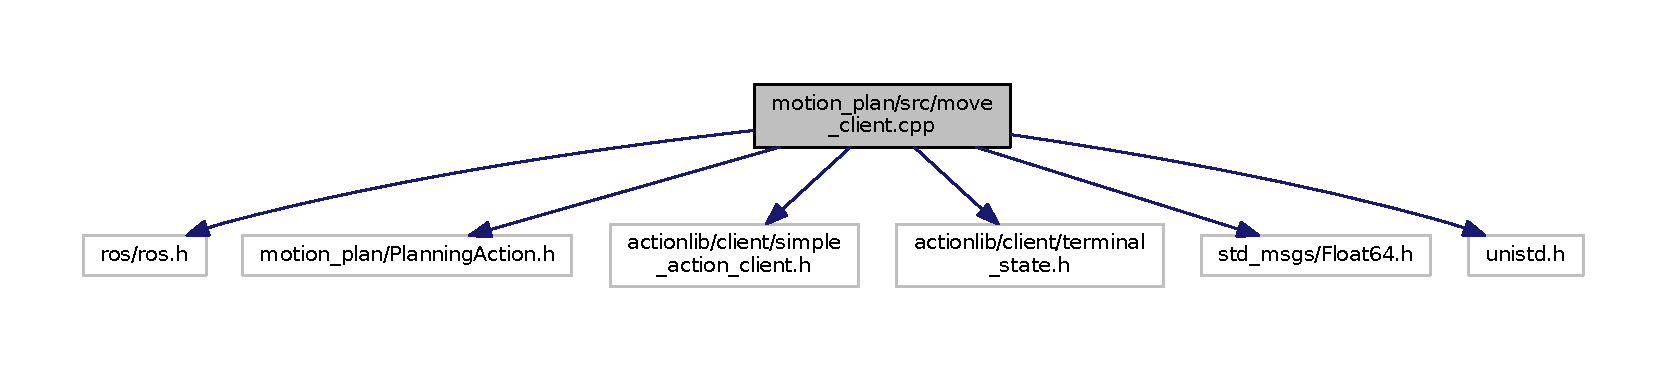
\includegraphics[width=350pt]{move__client_8cpp__incl}
\end{center}
\end{figure}
\subsection*{Functions}
\begin{DoxyCompactItemize}
\item 
int \hyperlink{move__client_8cpp_a3c04138a5bfe5d72780bb7e82a18e627}{main} (int argc, char $\ast$$\ast$argv)
\end{DoxyCompactItemize}


\subsection{Function Documentation}
\index{move\+\_\+client.\+cpp@{move\+\_\+client.\+cpp}!main@{main}}
\index{main@{main}!move\+\_\+client.\+cpp@{move\+\_\+client.\+cpp}}
\subsubsection[{\texorpdfstring{main(int argc, char $\ast$$\ast$argv)}{main(int argc, char **argv)}}]{\setlength{\rightskip}{0pt plus 5cm}int main (
\begin{DoxyParamCaption}
\item[{int}]{argc, }
\item[{char $\ast$$\ast$}]{argv}
\end{DoxyParamCaption}
)}\hypertarget{move__client_8cpp_a3c04138a5bfe5d72780bb7e82a18e627}{}\label{move__client_8cpp_a3c04138a5bfe5d72780bb7e82a18e627}

\hypertarget{README__DOXY_8md}{}\section{Output/\+R\+E\+A\+D\+M\+E\+\_\+\+D\+O\+XY.md File Reference}
\label{README__DOXY_8md}\index{Output/\+R\+E\+A\+D\+M\+E\+\_\+\+D\+O\+X\+Y.\+md@{Output/\+R\+E\+A\+D\+M\+E\+\_\+\+D\+O\+X\+Y.\+md}}

\hypertarget{README_8md}{}\section{R\+E\+A\+D\+M\+E.\+md File Reference}
\label{README_8md}\index{R\+E\+A\+D\+M\+E.\+md@{R\+E\+A\+D\+M\+E.\+md}}

%--- End generated contents ---

% Index
\backmatter
\newpage
\phantomsection
\clearemptydoublepage
\addcontentsline{toc}{chapter}{Index}
\printindex

\end{document}
